\documentclass[12pt,a4paper,twoside]{report}
\usepackage[italian]{babel}
\usepackage{newlfont}
\usepackage{color}
\textwidth=450pt\oddsidemargin=0pt

% INIZIO HEADER INSERITI DA ME

%\documentclass[12pt,a4paper]{article}
%\usepackage[utf8]{inputenc}
\usepackage{titling}
\usepackage[backend=bibtex,
			style=numeric-comp,
			sorting=none,
			url=false,
			isbn=false,
			doi=false,
			eprint=false,
			giveninits=true
			]{biblatex}
\newbibmacro{string+doiurlisbn}[1]{%
	\iffieldundef{doi}{%
		\iffieldundef{url}{%
			\iffieldundef{isbn}{%
				\iffieldundef{issn}{%
					#1%
				}{%
					\href{http://books.google.com/books?vid=ISSN\thefield{issn}}{#1}%
				}%
			}{%
				\href{http://books.google.com/books?vid=ISBN\thefield{isbn}}{#1}%
			}%
		}{%
			\href{\thefield{url}}{#1}%
		}%
	}{%
		\href{http://dx.doi.org/\thefield{doi}}{#1}%
	}%
}
\DeclareFieldFormat{title}{\usebibmacro{string+doiurlisbn}{\mkbibemph{#1}}}
\DeclareFieldFormat[article,book,conference,phdthesis,misc]{title}%
{\usebibmacro{string+doiurlisbn}{\mkbibquote{#1}}}
\renewbibmacro{in:}{}
\addbibresource{bibliography.bib} %Import the bibliography file
%\setlength{\droptitle}{-2cm}% change title position
\usepackage{amsmath}
\newcommand{\matr}[1]{\boldsymbol{#1}}
\newcommand{\transp}[1]{{#1}^{\mathsf{T}}}
\newcommand{\vect}[1]{\boldsymbol{#1}}
%\usepackage{amsfonts}
\usepackage[style=american]{csquotes}
\usepackage{amssymb}
\usepackage{siunitx}
\usepackage[export]{adjustbox}[2011/08/13]
%\usepackage[T1]{fontenc}
\usepackage{tablefootnote}
\usepackage{multirow}
\usepackage{array}
\newcolumntype{P}[1]{>{\centering\arraybackslash}p{#1}}
\newcolumntype{M}[1]{>{\centering\arraybackslash}m{#1}}
\newenvironment{dedication}{
	\clearpage           % we want a new page
	\thispagestyle{empty}% no header and footer
	\vspace*{\stretch{1}}% some space at the top
	\itshape             % the text is in italics
	\raggedleft          % flush to the right margin
}
{\par % end the paragraph
	\vspace{\stretch{3}} % space at bottom is three times that at the top
	\clearpage           % finish off the page
}
\usepackage{graphicx}
\graphicspath{{images/}}
\usepackage[version=4]{mhchem}
\usepackage[toc,page]{appendix}
\renewcommand\appendixname{Appendice}
\renewcommand\appendixtocname{Appendice}
\renewcommand\appendixpagename{Appendice}
%\usepackage{siunitx}
\usepackage{float}
\usepackage[top=1.7in,left=1in,right=1in]{geometry}
%\usepackage{listings}
%\usepackage{circuitikz}
\usepackage{tikz-feynman}
\tikzfeynmanset{warn luatex=false,%disable warn for not using luatex
	compat=1.1.0}
\usepackage{subcaption}
\usepackage{tabularx}
%\renewcommand{\lstlistingname}{Code}
%\renewcommand{\lstlistlistingname}{List of Code}
%\lstdefinestyle{chstyle}{
	%	backgroundcolor=\color{gray!12},
	%	basicstyle=\ttfamily\small,
	%	commentstyle=\color{green!60!black},
	%	keywordstyle=\color{magenta},
	%	stringstyle=\color{blue!50!red},
	%	showstringspaces=false,
	%	%captionpos=b,
	%	numbers=left,
	%	numberstyle=\footnotesize\color{gray},
	%	numbersep=10pt,
	%	%stepnumber=2,
	%	tabsize=2,
	%	frame=L,
	%	framerule=1pt,
	%	rulecolor=\color{red},
	%	breaklines=true,
	%	inputpath=code
	%}
%\renewmenumacro{\directory}{pathswithfolder} % default: path
%\renewmenumacro{\keys}{shadowedroundedkeys} % default: roundedkeys
\setlength{\arrayrulewidth}{0.9pt}
\renewcommand{\arraystretch}{1.3}
\usepackage{mathcomp}

%\usepackage{fontspec}
%\setmainfont{Calibri}

\usepackage{fancyhdr}
\pagestyle{fancy}
%\renewcommand{\chaptermark}[1]{\markboth{\MakeUppercase{\chaptername\ \thechapter.\ #1}}{}}
\renewcommand{\chaptermark}[1]{\markboth{\MakeUppercase{CAP.\ \thechapter\ --\ #1}}{}}
\setlength{\headwidth}{15cm} % la larghezza delle tabelle è di 1 cm inferiore (14cm)
\fancyhead{} % clear all header fields
\fancyhead[LO]{\footnotesize \textsl{\rightmark}}
\fancyhead[RE]{\footnotesize \textsl{\leftmark}}
\fancyhead[LE,RO]{\footnotesize \thepage}
\fancyfoot{} % clear all footer fields
\renewcommand{\headrulewidth}{0.3pt}

\usepackage{setspace}% di default è interlinea singola

\newsavebox{\largestimage}

%\usepackage[font=it]{caption}
%\usepackage{indentfirst}
%\interfootnotelinepenalty=10000

\usepackage{hyperref}
\hypersetup{
	colorlinks,
	citecolor=black,
	filecolor=black,
	linkcolor=black,
	urlcolor=black
}

% FINE HEADER INSERITI DA ME

\begin{document}
	\pagenumbering{roman}
	\begin{titlepage}
		\begin{center}
			{{\Large{\textsc{Alma Mater Studiorum $\cdot$ Universit\`a di Bologna}}}} 
			\rule[0.1cm]{15.8cm}{0.1mm}
			\rule[0.5cm]{15.8cm}{0.6mm}
			\\\vspace{3mm}
			
			{\small{\bf Scuola di Scienze \\ 
					Dipartimento di Fisica e Astronomia\\
					Corso di Laurea in Fisica}}
			
		\end{center}
		
		\vspace{23mm}
		
		\begin{center}
			\doublespacing
			{\LARGE{\bf IDENTIFICAZIONE DEI FRAMMENTI NUCLEARI PRODOTTI IN EVENTI SIMULATI ALL'ESPERIMENTO FOOT}}\\
		\end{center}
		
		\vspace{35mm} \par \noindent
		
		\begin{minipage}[t]{0.47\textwidth}
			%
			% INSERIRE IL NOME DEL RELATORE CON IL RELATIVO TITOLO DI DOTTORE O PROFESSORE
			%
			{\large{\bf Relatore: \vspace{3mm}
					
					Prof. Roberto Spighi}}
		\end{minipage}
		%
		\hfill
		%
		\begin{minipage}[t]{0.47\textwidth}\raggedleft {
				{\large{\bf Presentata da:
						\vspace{3mm}\\
						Simone Pasquini}}}
		\end{minipage}
		
		\par
		\vspace{\baselineskip}
		
		\begin{minipage}[t]{0.47\textwidth}
			%
			% INSERIRE IL NOME DEL RELATORE CON IL RELATIVO TITOLO DI DOTTORE O PROFESSORE
			%
			{\large{\bf Correlatore: \vspace{3mm}
					
					Dott. Roberto Zarrella}}
		\end{minipage}
		
		\vspace{45mm}
		
		\begin{center}
			Anno Accademico { 2023/2024}
		\end{center}
		
	\end{titlepage}
	\newpage
	\newgeometry{top=4cm,bottom=4cm,left=3cm,right=3cm}% Cambia questi margini per spostare a destra o a sinistra le pagine pari o dispari
	\onehalfspacing % Also singlespacing, doublespacing
	\begin{dedication}
		PROVA
	\end{dedication}
	\chapter*{Sommario}
	L'adroterapia è una tecnica utilizzata nelle cure oncologiche e consiste nell'irradiare una regione cancerosa con un fascio di particelle adroniche, per creare danni irreparabili al DNA delle cellule tumorali. Penetrando nel corpo umano, tali particelle rilasciano un'elevata quantità di energia nella regione del picco di Bragg, situata in prossimità della massima profondità raggiunta dalle particelle nei tessuti, mentre il rilascio nel canale di ingresso è piuttosto basso. Tali caratteristiche rendono l'adroterapia più adatta per trattamento di tumori profondi rispetto alle tecniche radioterapiche convenzionali, poiché il profilo di dose dell'adroterapia massimizza i danni biologici nella zona tumorale e li limita negli organi sani adiacenti. Il problema principale dell'adroterapia risiede nei processi di frammentazione nucleare che avvengono tra il fascio incidente e i nuclei del corpo umano. Infatti, vista la complessità nel rivelare i frammenti secondari prodotti dalle interazioni nucleari, risulta altrettanto difficile determinare con accuratezza l'energia rilasciata dai frammenti stessi e, di conseguenza, i danni biologici che potrebbero provocare nel corpo umano. Per tali motivi, nel $2017$ è nato FOOT, un esperimento il cui scopo principale è quello di misurare le sezioni d'urto differenziali rispetto all'energia e all'angolo di emissione dei frammenti prodotti nelle interazioni nucleari che intercorrono tra il fascio adroterapico e la regione tissutale irradiata. In questo lavoro di tesi si analizzano i dati ottenuti da simulazioni Monte Carlo in cui un bersaglio di grafite al \ce{^{12}C} viene irradiato da un fascio di ioni \ce{^{12}C} di energia cinetica di $200 \mbox{ MeV/u}$. Attraverso un programma di analisi si identificano gli isotopi dei frammenti maggiormente prodotti mediante la ricostruzione dei loro numeri atomici $Z$ e di massa $A$. Si ottengono stime di $Z$ con una precisione percentuale che va dal $5.3\%$ dell'idrogeno \ce{H} al $2.3\%$ del carbonio \ce{C}, mentre le misure del numero di massa $A$, ottenute mediante tre modalità differenti, possiedono una risoluzione percentuale che va dall'$1.4\%$ del carbonio \ce{^{12}C} all'$8.9\%$ del berillio \ce{^{9}Be}.
	\newpage
	\tableofcontents
	\newpage
	\chapter*{Introduzione}
	\markboth{INTRODUZIONE}{INTRODUZIONE}
	\addcontentsline{toc}{chapter}{Introduzione}
	La conoscenza scientifica e le tecniche sperimentali sviluppate nei progetti di ricerca della fisica fondamentale hanno permesso, nel corso del tempo, un crescente coinvolgimento della fisica in molteplici ambiti del sapere, dall'intelligenza artificiale alla medicina, dai beni culturali ai cambiamenti climatici. Ciò è stato possibile grazie alla naturale interdisciplinarità della scienza e dei suoi metodi, determinanti per il sistema sociale, economico e politico attuale. In questa tesi l'obiettivo è lo studio dei processi di frammentazione nucleare prodotti dall'interazione di adroni e nuclei con la materia, interessanti non solo per la fisica fondamentale, ma anche nelle applicazioni mediche, dall'adroterapia alla radioprotezione spaziale.
	
	L'argomento principale della tesi è l'adroterapia, una tecnica che prevede l'impiego di fasci di particelle adroniche cariche, come protoni e ioni carbonio, in ambito oncologico. Rispetto alle tecniche di radioterapia convenzionali, l'adroterapia risulta più favorevole in quanto gli adroni rilasciano la maggior parte della loro energia in una regione piuttosto limitata del corpo umano (picco di Bragg); l'aspetto cruciale è la possibilità di fissare il punto di massimo rilascio modificando l'energia del fascio. Gli scienziati, riconoscendo le peculiarità del profilo di dose adroterapico, impiegano attualmente l'adroterapia non solo nella cura dei tumori più profondi, ma anche nei trattamenti oncologici più delicati in cui è necessario risparmiare gli organi vitali attorno alla sede tumorale. In Italia i vantaggi dell'adroterapia nella cura delle neoplasie hanno permesso che tale terapia nel $2017$ entrasse a far parte dei livelli essenziali di assistenza previsti dal Servizio Sanitario Nazionale (SSN). Nonostante l'adroterapia rappresenti un terreno molto fertile nell'ambito delle cure oncologiche, i processi di frammentazione nucleare tra i nuclei del fascio e quelli del corpo umano costituiscono un rischio per le cure adroterapiche, dato che i frammenti secondari prodotti rilasciano energia in zone tipicamente sane. La frammentazione provoca danni biologici nocivi per il paziente che, se non opportunamente considerati all'interno dei piani di trattamento, renderebbero l'adroterapia una tecnica molto meno efficace.
	
	Lo scopo della radioprotezione spaziale è quello di sviluppare materiali che possano schermare l'effetto nocivo che le radiazioni ionizzanti, dovute soprattutto ai raggi cosmici o alle SPE, inducono sull'uomo. Negli ultimi anni il tema della radioprotezione ha destato particolare attenzione, specialmente per l'interesse da parte delle agenzie spaziali private e pubbliche nell'intraprendere missioni umane di lunga durata al di fuori dell'atmosfera. A differenza dell'adroterapia, i processi di frammentazione nucleare non avvengono solo nel corpo umano, ma anche nei materiali utilizzati per la schermatura dalle radiazioni ionizzanti del cosmo, la cui progettazione deve tenerne conto e minimizzarne gli effetti.
	
	Le applicazioni sopra descritte motivano da tempo lo studio dei processi di frammentazione nucleare, sebbene fino ad ora sia stato molto complesso misurare le sezioni d'urto dei frammenti secondari, sia per la rarità di tali eventi sia perché i frammenti in alcuni casi possiedono un range dell'ordine dei $\mu\mbox{m}$ che ne impedisce la rivelazione. In particolare, i processi di frammentazione nucleare tipici dei range energetici delle applicazioni adroterapiche ($50$--$250\mbox{ MeV}$ per i protoni e $50$--$400\mbox{ MeV/u}$ per gli ioni carbonio) presentano evidenti lacune sperimentali che vengono compensate dall'impiego di simulazioni Monte Carlo, che comunque necessitano di una continua implementazione basata su dati reali affidabili. L'impellente necessità di colmare la mancanza di misure ha portato l'Istituto Nazionale di Fisica Nucleare (INFN) ad approvare nel $2017$ l'esperimento FOOT (FragmentatiOn Of Target), il cui scopo principale è quello di misurare la sezione d'urto, l'energia e la direzione di produzione dei frammenti secondari generati dalle interazioni nucleari tra particelle cariche e nuclei del corpo umano (in caso di studi di adroterapia) o di materiali vari (per la protezione spaziale).
	
	La tesi è strutturata in tre capitoli. Nel \hyperref[cap:1]{Cap. 1} si analizzano le principali caratteristiche delle interazioni ionizzanti con la materia e gli effetti biologici che inducono sul corpo umano, con particolare attenzione alle differenze tra le tecniche di radioterapia convenzionale e adroterapia. Nel \hyperref[cap:2]{Cap. 2} si presenta l'apparato sperimentale di FOOT, il suo funzionamento e le modalità con cui avviene la rivelazione dei frammenti nucleari. Nel \hyperref[cap:3]{Cap. 3} si affronta una fase preliminare dell'analisi dati di FOOT, vale a dire l'identificazione univoca dei frammenti prodotti dalle interazioni nucleari, che avviene misurando i loro numeri atomici e di massa. Nello specifico, si crea un programma con cui si analizzano i dati ottenuti da simulazioni Monte Carlo che, combinando le grandezze cinematiche dei frammenti ottenute dai rivelatori, consentono di stimare i numeri atomici e di massa dei frammenti stessi, dopo un'opportuna applicazione di fit gaussiani e selezioni che consentono di eliminare eventuali artefatti della ricostruzione.
	\newpage
	\pagenumbering{arabic}
	\chapter{Terapie oncologiche e radiazioni ionizzanti}\label{cap:1}
	\section{Incidenza tumorale nel mondo}\label{sec:1.1}
	Tra le principali cause di morte della popolazione mondiale è possibile annoverare le neoplasie (o tumori) ovvero neoformazioni che, a causa di mutazioni genetiche che sfuggono ai meccanismi di controllo della proliferazione cellulare, iniziano a crescere, senza alcuna finalità, in maniera incontrollata e scoordinata rispetto al tessuto sano. \`E possibile distinguere due tipi di neoplasie: benigne e maligne. Mentre le prime si limitano alla sede di origine, le seconde generano metastasi, un processo in cui le cellule neoplastiche si spostano dalla sede originaria e danno origine a masse anomale che invadono altri tessuti dell'organismo, ostacolandone le funzioni vitali. In quest'ultimo caso si parla di tumore maligno o cancro.
	
	Sebbene sia possibile prevenire fino al $50\%$\footnote{Tale percentuale varia fortemente in base al tipo di tumore e alla tempestività della diagnosi.} dei tumori evitando fattori di rischio e implementando strategie di profilassi già esistenti \cite{who}, si stima che nei Paesi industrializzati\footnote{Si fa riferimento ai Paesi OCSE (Organizzazione per la Cooperazione e lo Sviluppo Economico).} il cancro è la seconda causa di morte (causando il $21\%$ dei decessi totali nel $2021$), preceduto solo dalle malattie cardiovascolari \cite{oecd2023}. Nonostante il tasso di mortalità dovuto alle patologie tumorali sia sceso sin dal $2000$, nel $2022$ i casi diagnosticati di cancro a livello mondiale si sono attestati a quasi $20.0$ milioni (pari al $2.5\tcperthousand$ della popolazione totale \cite{unicef2022}), il $48.8\%$ dei quali ha portato alla morte del paziente\footnote{Negli ultimi dieci anni il numero di casi di tumore è aumentato di anno in anno, soprattutto a causa dell'invecchiamento progressivo della popolazione \cite{De_Angelis2024-no}, ma nel biennio $2020$-$2021$ il trend è cambiato a causa della pandemia di COVID-$19$ che ha precluso l'accesso a screening oncologici (nel periodo gennaio--ottobre $2020$ vi è stato un calo del $37.3\%$ di test diagnostici rispetto al periodo pre-pandemico) \cite{Angelini2023-xc}. Ciò potrebbe aumentare i tassi di incidenza e mortalità dei tumori, rivelandosi fatale nel medio-lungo termine \cite{oecd2021}.} \cite{gco}. Inoltre, il tasso di mortalità dovuto alle patologie tumorali è strettamente legato all'ISU (Indice di Sviluppo Umano) dei Paesi, variando dal $39.2\%$ per i Paesi con ISU molto alto al $67.1\%$ per quelli con basso ISU \cite{gco}.
	
	Altri fattori, quali il sesso e l'età, riducono ulteriormente l'uniformità dei tassi di incidenza e mortalità delle malattie tumorali. Infatti, a livello globale, l'incidenza di cancro negli uomini risulta più alta dell'$8.0\%$ rispetto a quella delle donne \cite{gco2}, divario dovuto anche alla maggiore esposizione dei primi a fattori di rischio, come fumo e consumo di alcol. Inoltre, il $58\%$ delle diagnosi di tumore riguarda persone con più di $65$ anni di età \cite{uscs}.
	
	Sebbene i dati sopra citati testimonino la gravità delle patologie oncologiche, è indubbio che il progresso della scienza degli ultimi anni abbia permesso un notevole sviluppo nell'efficacia dei trattamenti oncologici; basti pensare che nel decennio $2010$--$2020$, in Paesi come l'Italia, gli Stati Uniti d'America, il Regno Unito e la Svizzera, il numero di persone sopravvissute dopo una diagnosi di cancro è aumentato approssimativamente del $3\%$ ogni anno \cite{Guzzinati2018-sf}.
	
	\section{Terapie oncologiche}\label{sec:1.2}
	Il trattamento di un tumore può avvenire in molti modi differenti che variano in base al tipo di cancro, al suo stadio di avanzamento e agli obiettivi che si intendono raggiungere al termine dei trattamenti. Oggigiorno le terapie oncologiche si distinguono in locali (o regionali) e generali (o sistemiche) in base all'estensione del tumore che colpisce il paziente. Al primo gruppo appartengono terapie come la chirurgia, la radioterapia e l'adroterapia, mentre al secondo afferiscono la chemioterapia e l'immunoterapia. Tali tecniche, proprio per la loro diversità, sono spesso utilizzate in maniera complementare per aumentare l'efficacia dei trattamenti clinici. Per pianificare il trattamento più adeguato a fronte di una certa patologia oncologica, si introduce il concetto di stadiazione, che è un modo di descrivere in maniera schematica, rigorosa e standardizzata la grandezza di un tumore e la sua diffusione al di fuori della sede originale \cite{airc}. Le informazioni tipiche fornite dalla stadiazione includono la collocazione del tumore, la sua estensione e la sua eventuale diffusione in parti del corpo differenti. Infatti, come già accennato, le cellule tumorali si moltiplicano in modo incontrollato andando a occupare (per mezzo del sistema linfatico o sanguigno) organi e tessuti distanti dalla sede di sviluppo originaria, attraverso un fenomeno chiamato metastatizzazione. Chiaramente ciascuna terapia possiede effetti collaterali specifici, correlati all'azione distruttiva impiegata per debellare la malattia oncologica.
	
	Se il tumore ha raggiunto un'estensione tale da formare metastasi, si scelgono trattamenti sistemici in modo che si possa debellare o, quantomeno, contenere la sua diffusione. La chemioterapia consiste nella somministrazione di uno o più farmaci citotossici (o antiblastici) capaci di aggredire le cellule cancerose \cite{aimac1}, mentre nell'immunoterapia si tenta di istruire il sistema immunitario affinché possa riconoscere ed eliminare le cellule malate che, in assenza di trattamenti clinici esterni, appaiono ``nascoste'' al sistema immunitario stesso.
	
	Qualora il tumore fosse localizzato, ben raggiungibile dall'esterno e sufficientemente lontano da organi vitali, si ricorre a operazioni chirurgiche, con le quali si asporta la massa tumorale dal corpo del paziente. Solitamente, prima o dopo l'operazione chirurgica, si procede con tecniche radioterapiche, adroterapiche o chemioterapiche in base alle necessità. Ad esempio, nella radioterapia neoadiuvante il trattamento radioterapico viene effettuato prima dell'intervento chirurgico, mentre nella radiochemioterapia concomitante si eseguono sessioni di chemioterapia e radioterapia a seguito dell'operazione chirurgica \cite{aimac2}. In generale, la commistione di suddette tecniche consente di rimuovere le cellule tumorali sfavorendo eventuali recrudescenze della malattia.
	
	Nel caso in cui la massa tumorale non risulti rimovibile attraverso un'operazione chirurgica, per esempio a causa della sua localizzazione anatomica,\footnote{\`E il caso di neoplasie che colpiscono organi o tessuti la cui rimozione sarebbe troppo invalidante per il paziente \cite{foot_site}.} si preferisce ricorrere alla radioterapia e all'adroterapia, ove quest'ultima è una tecnica avanzata di radioterapia. Pur non essendo invasive come la chirurgia, tali terapie consentono di danneggiare specifici tessuti biologici malati utilizzando radiazione ionizzante\footnote{Una radiazione si dice ionizzante quando ha energia sufficiente a liberare gli elettroni legati agli atomi della materia in cui penetra. La ionizzazione provoca danni biologici ai tessuti del corpo umano.} composta da fasci di fotoni ed elettroni in radioterapia e da particelle adroniche (come protoni, neutroni e ioni) in adroterapia (si veda \hyperref[fig:simulation]{Fig. 1.1}). In particolare, lo scopo di entrambi i trattamenti è quello di depositare una quantità di energia per unità di massa (detta dose) sufficiente a provocare un danno biologico che inibisca la crescita del tumore con effetti collaterali minimi \cite{asimmetrie_curareCLP}. Sebbene sembrino molto simili, la radioterapia e l'adroterapia presentano caratteristiche fisiche e radiobiologiche molto dissimili, i cui dettagli verranno evidenziati nel prosieguo della trattazione. Una delle differenze più evidenti è che la dose di un fascio radioterapico viene rilasciata in una regione piuttosto ampia, non concentrata, mentre le particelle adroniche, penetrando nei tessuti in grande profondità, irradiano un'ingente quantità di energia in uno spazio molto limitato definito picco di Bragg. In altre parole, le tecniche adroterapiche riducono il rischio di distruggere cellule sane situate prima e dopo il tumore in quanto permettono di definire in modo molto più preciso la regione da irradiare \cite{foot_site}. In definitiva, l'adroterapia consente sia di distruggere più efficacemente porzioni di cellule tumorali situate in profondità sia di minimizzare i danni a carico dei tessuti sani circostanti \cite{cnao1}, una duplice funzione in grado di migliorare la qualità della vita del paziente.
	\begin{figure}[H]
		\centering
		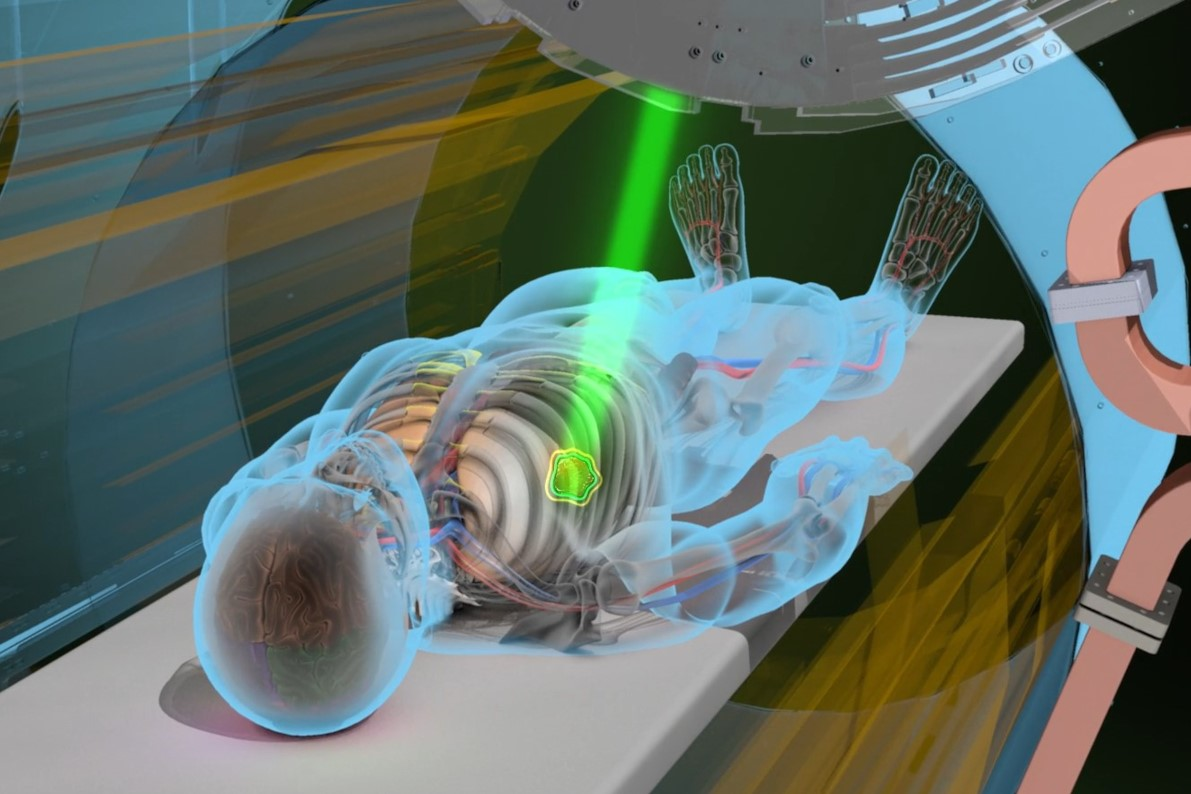
\includegraphics[width=0.95\linewidth]{simulation.jpg}
		\caption{Simulazione di un irraggiamento radioterapico o adroterapico sul corpo di un paziente \cite{treatment_photo}.}
		\label{fig:simulation}
	\end{figure}
	Sebbene l'adroterapia sia complessivamente più efficace rispetto alla radioterapia nella distruzione di cellule tumorali e nella salvaguardia dei tessuti sani, è un trattamento relativamente recente (si veda \hyperref[sec:storia_adroterapia]{Sez. 1.3.1}) che, tra le varie e complesse strutture, necessita di acceleratori di particelle, il cui costo varia tra $15$--$150$ milioni di euro, molto maggiore della strumentazione radioterapica il cui costo generalmente non supera i $10$ milioni di euro; pertanto, l'adroterapia è meno sviluppata e più costosa della radioterapia. Inoltre, attualmente non sono ancora state misurate con sufficiente precisione le probabilità di avere effetti nucleari tra il fascio e i nuclei del corpo umano (argomento principale dell'esperimento FOOT \cite{foot_site}); quindi, prima di procedere con trattamenti reali, si sono rese necessarie simulazioni per valutare gli effetti di rischio, sebbene queste siano caratterizzate da numerose incertezze \cite{foot_cdr}. Per questi motivi, il settore di ricerca adroterapico è molto attivo e coinvolge un crogiolo culturale di fisici, medici e biologi che studiano gli effetti delle radiazioni ionizzanti sulle cellule umane, analizzabili solo mediante un approccio interdisciplinare.
	
	L'adroterapia, però, non appartiene esclusivamente all'ambito della sperimentazione, ma costituisce una realtà interazionale nella cura dei tumori a tutti gli effetti. Infatti, alla fine del $2023$, quasi \num{410000} pazienti hanno effettuato trattamenti adroterapici a livello globale (di cui \num{350000} con protoni, \num{56000} con ioni carbonio e \num{3500} con elio, pioni e altre particelle), un numero tre volte superiore a quello di fine $2014$ \cite{PTCOG}. Pur essendo tali numeri incoraggianti, è necessario continuare a investire risorse nella ricerca in modo che esperimenti della caratura di FOOT possano rendere l'adroterapia un trattamento più diffuso e accessibile a tutti.
	
	\section{Storia della radioterapia}
	La storia della radioterapia ha inizio nel novembre del $1895$ con un singolare episodio di serendipità, il cui protagonista è il fisico tedesco Wilhelm C. von Röntgen ($1845$--$1923$), scopritore dei raggi X. Durante lo studio dei raggi catodici prodotti da un tubo di Crookes, Röntgen si accorse che della radiazione sconosciuta (denominata da lui stesso ``X'' poiché incognita fino a quel momento) riusciva a oltrepassare la lastra di vetro che ricopre lo strumento. Röntgen comprese sin da subito le grandi potenzialità dei neonati raggi X, osservando che tale radiazione era in grado di delineare la struttura interna dei materiali attraversati. Fu proprio il fisico tedesco a effettuare la prima radiografia alla mano di sua moglie (illustrata in \hyperref[fig:rongten]{Fig. 1.2}) dopo un'esposizione di $15$ minuti, un tempo molto lungo e rischioso essendo i raggi X un tipo di radiazione ionizzante. Le immediate applicazioni della scoperta di Röntgen in campo medico gli valsero il premio Nobel per la fisica nel $1901$ \cite{rontgen}.
	\begin{figure}[H]
		\centering
		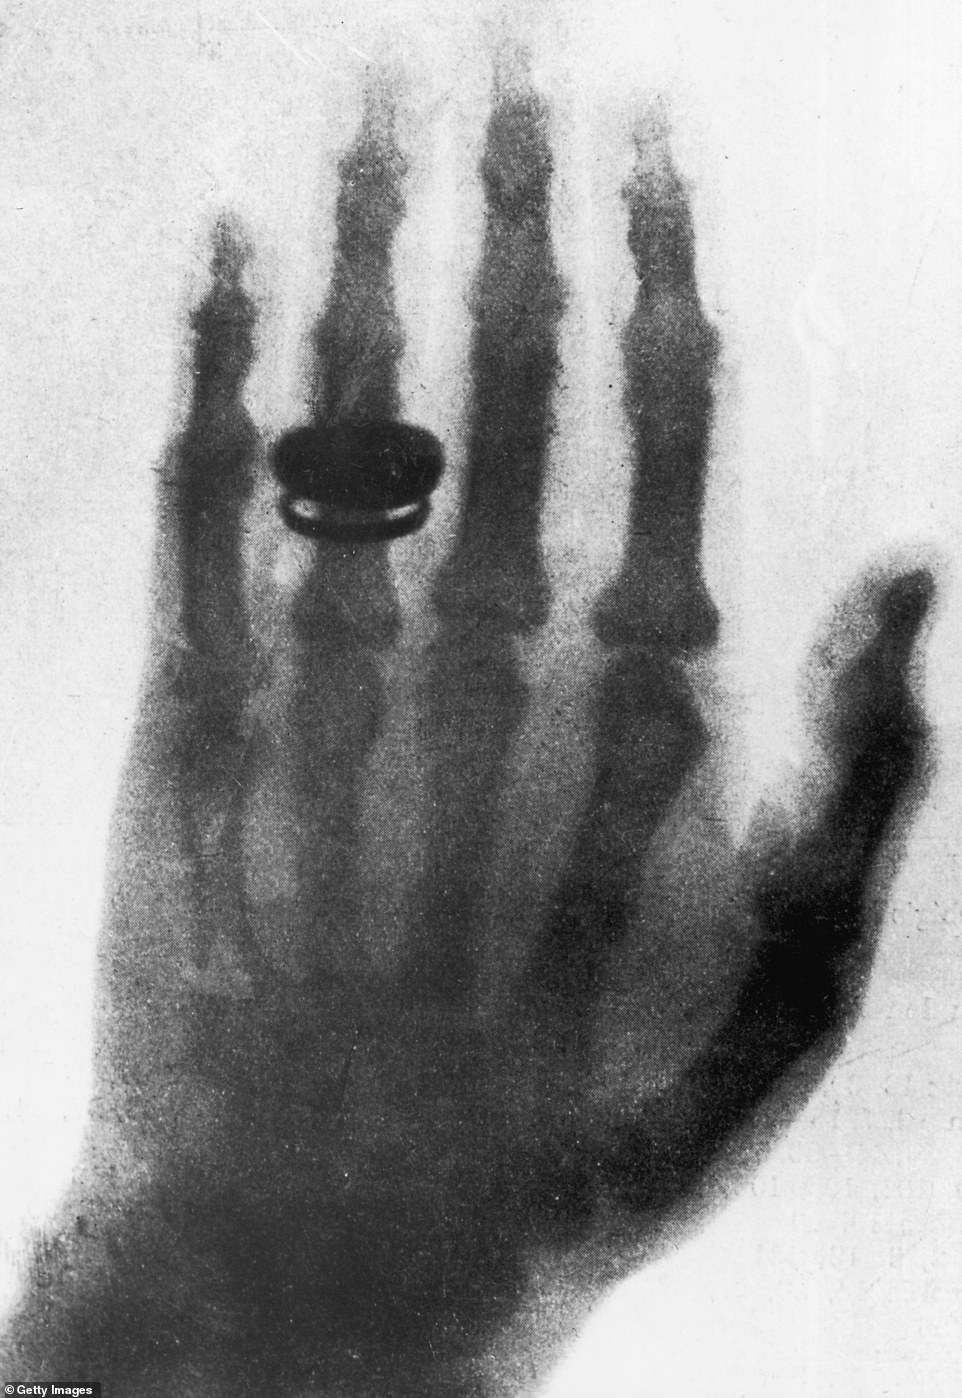
\includegraphics[width=0.4\linewidth]{rongten.jpg}
		\caption{Lastra a raggi X della mano di Anna B. Ludwig ($1839$--$1919$), moglie di Röntgen, avvenuta dopo $15$ minuti di esposizione \cite{hand_rongt_wife}.}
		\label{fig:rongten}
	\end{figure}
	Solamente un anno dopo la scoperta di Röntgen, Antoine H. Becquerel ($1852$--$1908$), studiando la fosforescenza dei sali di uranio, notò che alcuni materiali emettevano raggi elettromagnetici senza essere eccitati dalla luce solare. Becquerel scoprì così la radioattività spontanea dell'uranio, che gli valse il premio Nobel per la fisica nel $1903$ assieme ai coniugi Pierre Curie ($1859$--$1906$) e Maria Sklodowska ($1867$--$1934$) per la scoperta del radio \ce{^{226}Ra}. Da quel momento in avanti i raggi X furono impiegati nelle sperimentazioni terapeutiche, alcune delle quali portarono a svariati successi clinici (come la cura di vari lesioni cutanee dovute al \textit{lupus vulgaris} e al \textit{lupus eritematoso}).
	
	\subsection{Storia dell'adroterapia}\label{sec:storia_adroterapia}
	Dopo il rapido susseguirsi di scoperte dei primi anni del $1900$, vi fu l'avvento delle due Guerre Mondiali che, da un lato, rallentò il progresso della comunità scientifica, dall'altro rappresentò un'occasione utile ai popoli per sfoggiare il proprio avanzamento tecnico-scientifico. Il clima bellico lese l'internazionalismo scientifico di quegli anni, specialmente nel momento in cui venivano fondate le prime accademie internazionali delle scienze, come avvenne per la \textit{Kaiser Wilhelm Gesellschaft} di Berlino, il cui Istituto di Fisica ed Elettrochimica fu militarizzato dal ``generale in camice bianco'' Fritz Haber\footnote{Fritz Haber è noto ai più per aver vinto il premio Nobel nel $1918$ per la sintesi dell'ammoniaca, ripudiò le sue origini ebraiche mettendosi a servizio della Germania nazista durante il Primo Conflitto mondiale. Lo scienziato supervisionò l'impiego dell'iprite, un gas venefico da lui messo a punto, da parte dell'esercito tedesco nella nota battaglia di Ypres dell’aprile del $1915$, che fece strage delle truppe Alleate \cite{Smart1996-vt}.} ($1868$--$1934$), secondo il quale la scienza ``serve all’umanità in pace e alla patria in guerra'' \cite{Friedrich2017-wl,pietro_greco}.
	
	La corsa agli armamenti atomici degli anni successivi favorì un forte sviluppo della teoria atomica e nucleare, la cui conoscenza fu sfruttata dapprima come un'arma e solo in un secondo momento come una risorsa, impiegabile ad esempio nella cura di malattie. Un altro caso esemplare della dicotomia scientifica di quegli anni è rappresentato da Robert R. Wilson ($1914$--$2000$) che, dopo aver lavorato ai laboratori di Los Alamos per il Progetto Manhattan,\footnote{Il progetto Manhattan fu un programma di ricerca attivo dal $1942$ al $1946$ per la produzione della prima arma nucleare. Tale progetto viene tragicamente ricordato per la costruzione degli ordigni Little Boy e Fat Man con cui furono bombardate rispettivamente Hiroshima e Nagasaki.} nel $1946$ propose per primo l'utilizzo dei protoni nelle terapie oncologiche (notandone le grandi potenzialità rispetto alla radioterapia convenzionale \cite{Wilson1946-uk}) e nel $1967$ fondò il Fermilab (uno dei maggiori centri di ricerca odierni per la fisica delle particelle elementari). Wilson, misurando la dose rilasciata dai fasci di protoni prodotti dal ciclotrone del Lawrence Berkeley National Laboratory (LBL), notò che il picco di Bragg rendeva le terapie protoniche più efficienti dei metodi radioterapici utilizzati sino ad allora. Nell'articolo in ref. \cite{Wilson1946-uk}, lo scienziato fece anche rifermento a un possibile uso futuro degli ioni più pesanti, come gli ioni di carbonio, che ``potrebbero diventare terapeuticamente pratici''. Infatti, nel $1954$, nell'LBL si trattò il primo paziente utilizzando i protoni, a cui seguirono le prime terapie con elio nel $1957$ e con ioni di neon nel $1975$ \cite{amaldi_article}. Si sottolinea che in questi primi trattamenti, e in una buona parte dei successivi, le particelle venivano collimate senza sfruttare la loro carica elettrica, proprietà che sarebbe diventata fondamentale per la loro rivelazione e per il loro controllo attraverso campi magnetici.
	
	Un grande sviluppo della terapia protonica avvenne dopo la costruzione del ciclotrone di Harvard del $1949$ (in sostituzione del ciclotrone del $1937$ trasferito a Los Alamos per il Progetto Manhattan \cite{cerncourier}), col quale si ottennero numerosi successi, specialmente per il melanoma oculare e per i tumori ossei della base del cranio, che convinsero molti scienziati sulla superiorità dei protoni rispetto ai raggi X per i tumori vicini agli organi a rischio \cite{Wilson2004-tc}.
	
	Gli studi del ciclotrone di Harvard spinsero anche i laboratori russi e giapponesi ad avviare programmi di ricerca nella terapia adronica. Risulta di particolare importanza l'apertura del centro HIMAC (Heavy Ion Medical Accelerator in Chiba, si veda \hyperref[fig:himac]{Fig. 1.3}) \cite{hirao1992heavy} a Chiba (Giappone) che, nel $1994$, trattò per primo un paziente con un fascio di ioni carbonio, il cui rilascio di dose è nettamente superiore a quello di fotoni e protoni (si veda \hyperref[fig:photon]{Fig. 1.17}) e, per tale ragione, risulta più efficace nel controllo di tumori radioresistenti e di neoplasie più comuni (per esempio ai polmoni o al fegato).
	\begin{figure}[H]
		\centering
		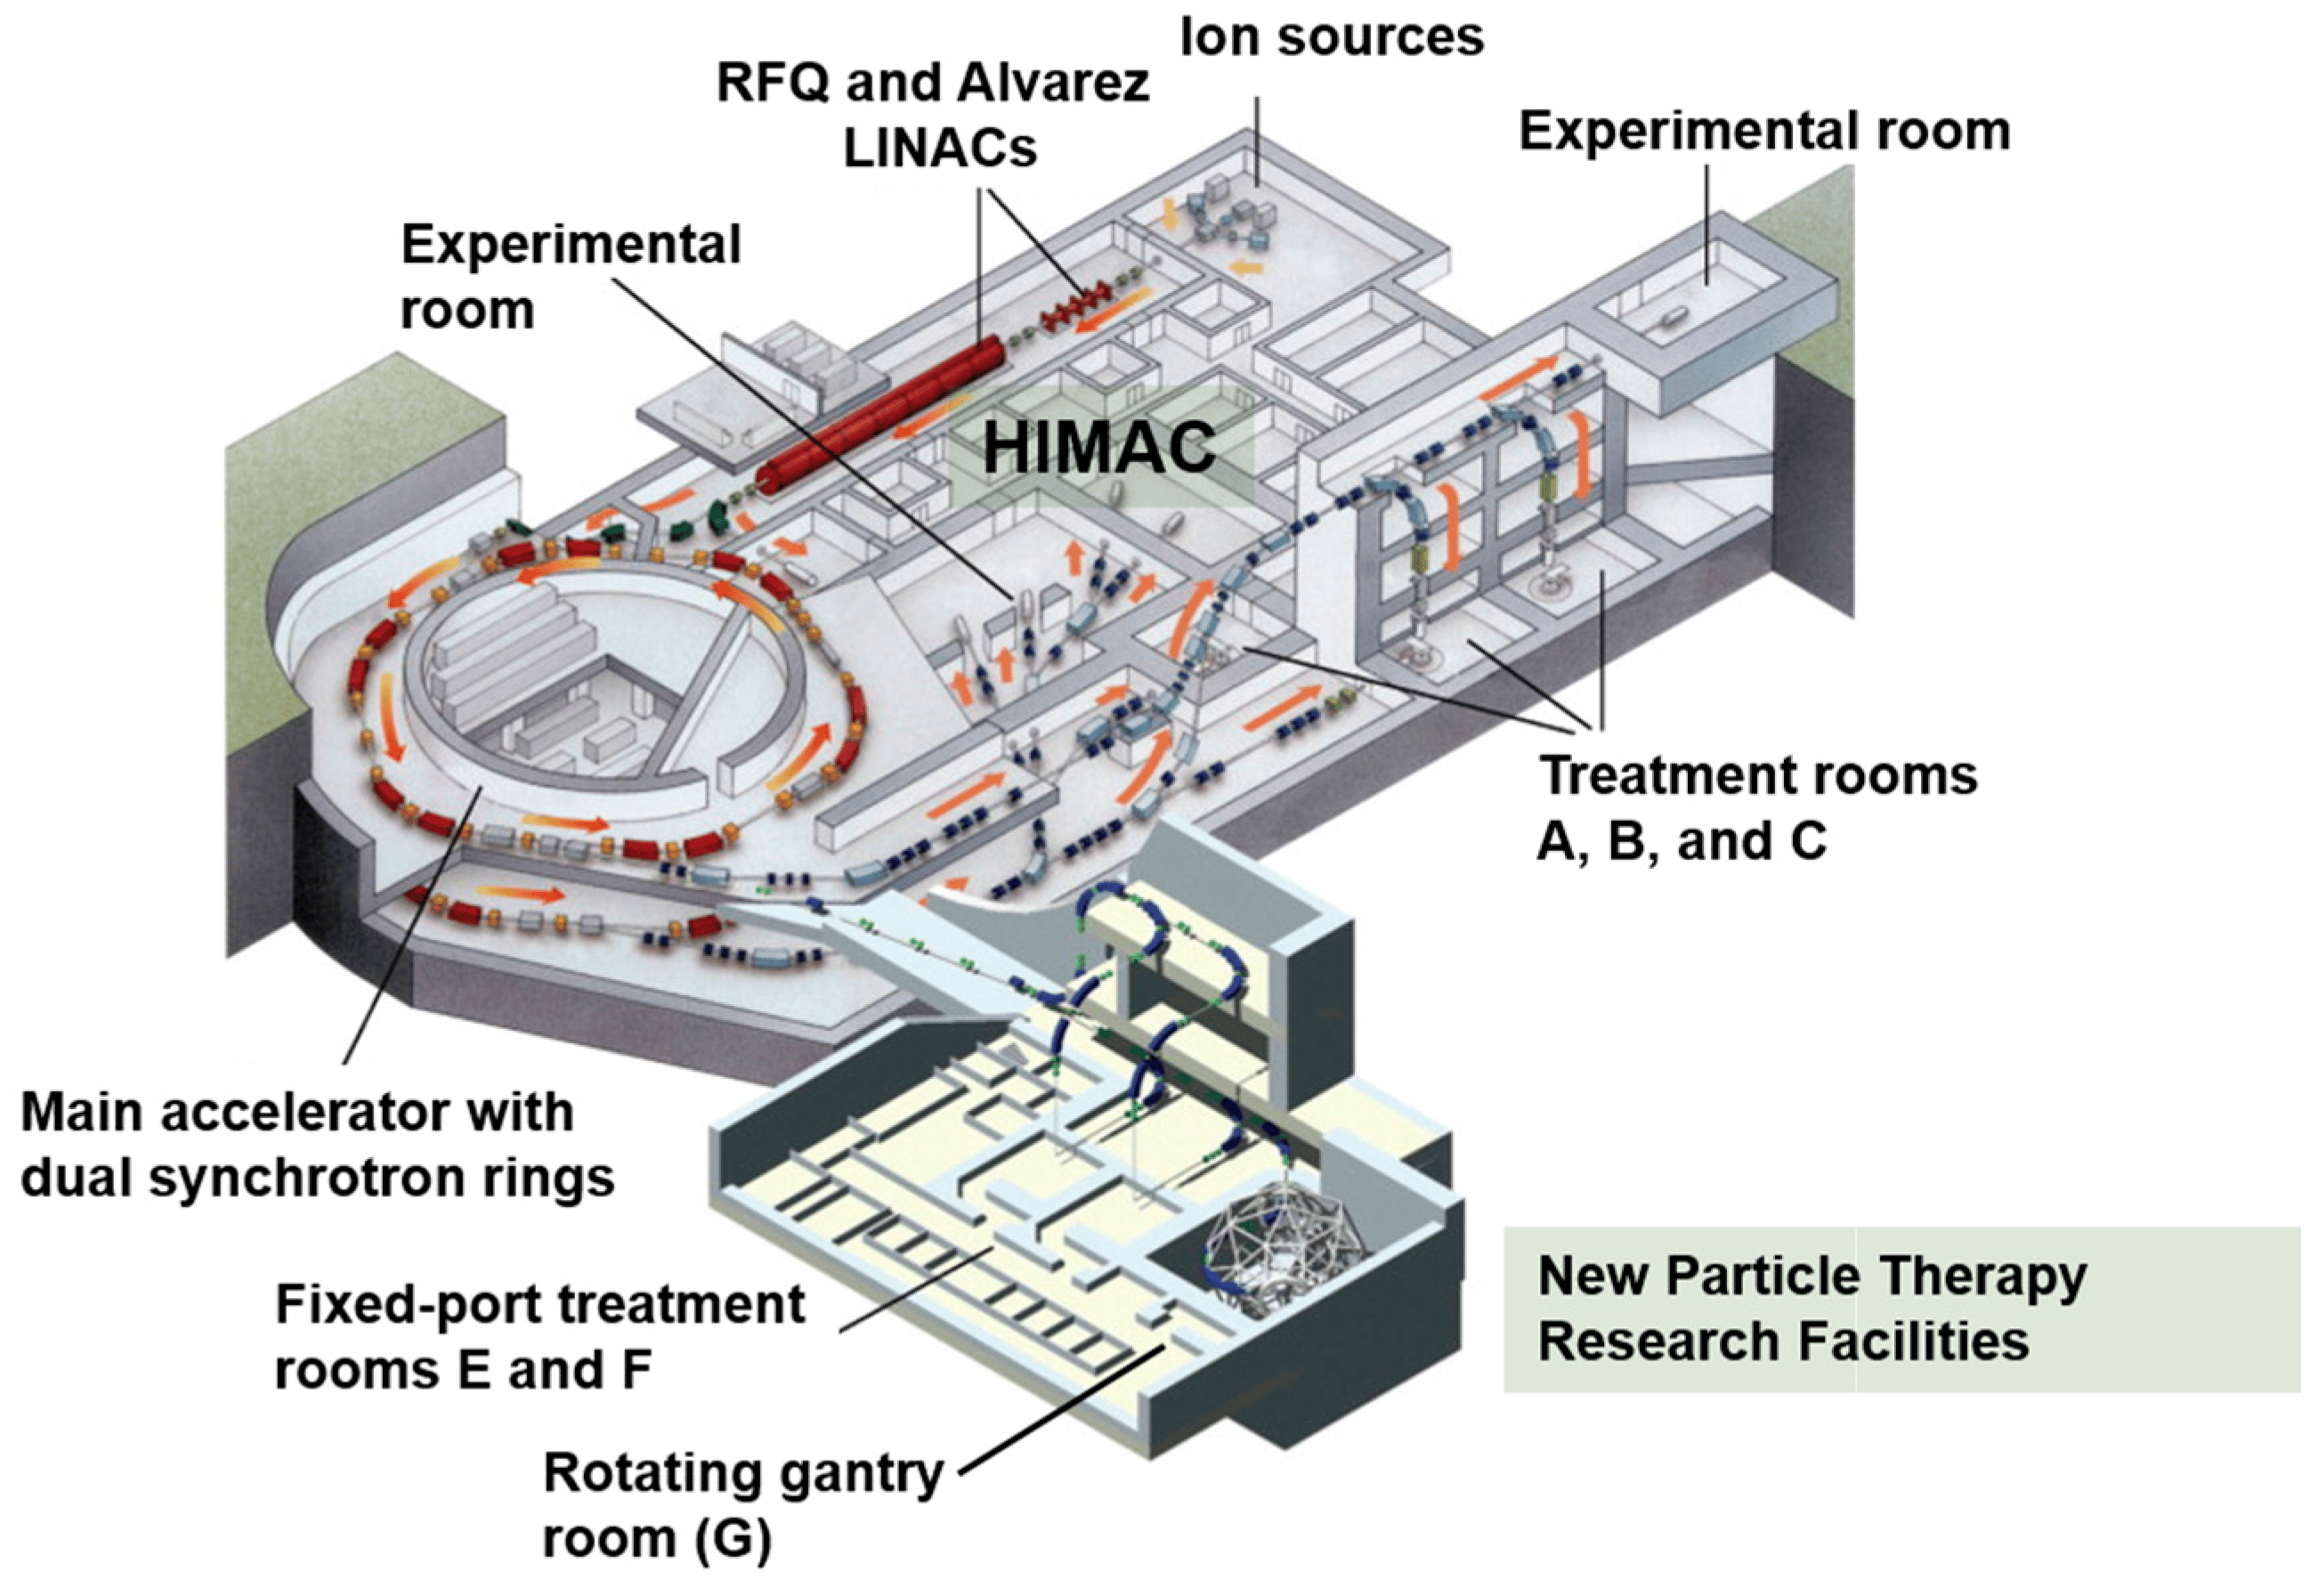
\includegraphics[width=0.7\linewidth]{himac.png}
		\caption{Panoramica delle strutture di ricerca HIMAC presso l'Istituto Nazionale di Scienze Radiologiche a Chiba \cite{cancers10030066}.}
		\label{fig:himac}
	\end{figure}
	La prima iniziativa completamente europea di un centro terapico agli ioni arrivò solo nel $1987$ con EULIMA (EUropean Light Ion Medical Accelerator). Il progetto prevedeva la costruzione di un sincrotrone\footnote{I ciclotroni, con diametro di circa $5\mbox{ m}$, si utilizzano per produrre fasci di protoni, mentre i sincrotroni, con diametro di oltre $10\mbox{ m}$, si usano principalmente per generare ioni carbonio \cite{asimmetrie_curareCLP}.} che, purtroppo, non fu mai costruito; si dovettero attendere progetti esclusivamente nazionali per un decisivo cambio di passo della terapia agli ioni. Solo nel decennio $1994$--$2004$ iniziò la costruzione di due centri nazionali fondamentali per i trattamenti con protoni e ioni carbonio: il primo è l'Heidelberg Ionenstrahl Therapy (HIT), aperto a Heidelberg (Germania) nel $2009$, il secondo, italiano, è il Centro Nazionale di Adroterapia Oncologica (CNAO) di Pavia, attivo sin dal $2011$ \cite{amaldi_article}.
	
	\subsection{Adroterapia in Italia}\label{sec:adroterapia_italia}
	Una delle figure più importanti per lo sviluppo dell'adroterapia in Italia è sicuramente il fisico italiano Ugo Amaldi ($1934$--). La sua lungimiranza ha portato l'Italia a essere la seconda nazione europea ad avere un centro adroterapico (il CNAO) capace di effettuare trattamenti con protoni e ioni carbonio (si pensi che attualmente ne esistono solo sei in tutto il mondo \cite{asimmetrie_curareCLP}). Nei paragrafi successivi si ripercorrono le principali tappe della storia dell'adroterapia in Italia.
	
	Nel $1991$, assieme al fisico medico Giampiero Tosi ($1937$--), Amaldi scrisse un articolo pionieristico in cui si proponeva un centro nazionale di terapia con particelle \cite{amaldi1991per}, idea accolta con entusiasmo dal noto oncologo Umberto Veronesi ($1925$--$2016$) e dall'allora Presidente dell'Istituto Nazionale di Fisica Nucleare (INFN) Nicola Cabibbo ($1935$--$2010$). Un anno dopo, fu istituita la fondazione TERA (TErapia con Radiazioni Adroniche) il cui duplice scopo era quello di costruire centri adroterapici in Italia e in Europa \cite{amaldi_article}.
	\begin{figure}[H]
		\centering
		\savebox{\largestimage}{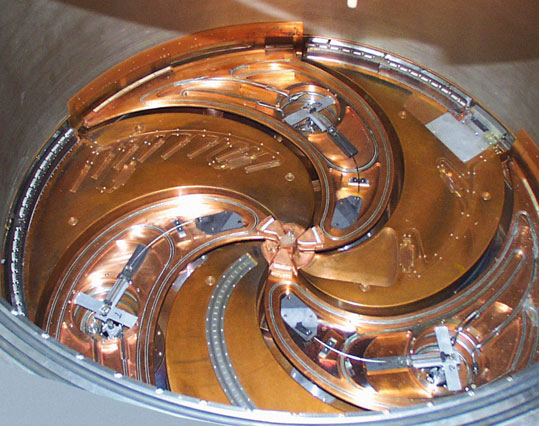
\includegraphics[width=0.49\textwidth]{catana1.jpg}}
		\begin{subfigure}[b]{0.49\textwidth}
			\centering
			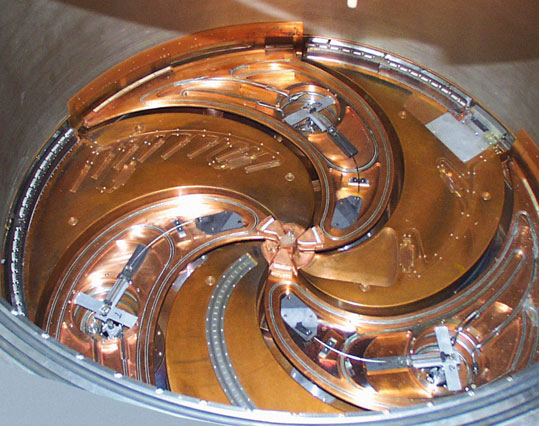
\includegraphics[width=\textwidth, scale=0.5]{catana1.jpg}
			\caption{Particolare interno del ciclotrone del CATANA \cite{asimmetrie_catana}.}
			\label{fig:catana1}
		\end{subfigure}
		\hfill
		\begin{subfigure}[b]{0.49\textwidth}
			\centering
			\raisebox{\dimexpr.5\ht\largestimage-.5\height}{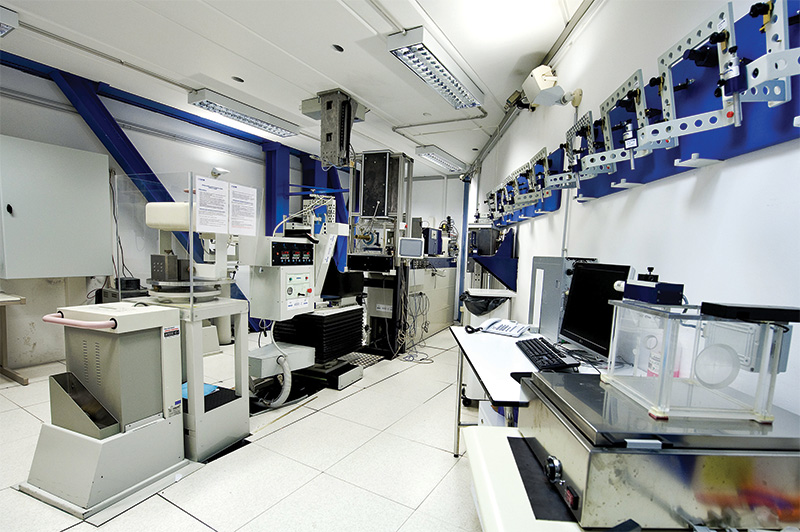
\includegraphics[width=\textwidth, scale=0.5]{catana2.jpg}}
			\caption{Attrezzatura presso la sala di trattamento del CATANA \cite{asimmetrie_DLAS}.}
			\label{fig:catana2}
		\end{subfigure}
		\caption{Immagini relative al CATANA dei LNS, primo centro di protonterapia in Italia.}
		\label{fig:catana}
	\end{figure}
	Alla fine del $1995$ si decise finalmente di creare una struttura protonterapica ai Laboratori Nazionali del Sud (LNS) sfruttando il ciclotrone superconduttore già attivo nei LNS. Il progetto, chiamato CATANA (Centro di AdroTerapia ed Applicazioni Nucleari Avanzate, \hyperref[fig:catana]{Fig. 1.4}), prevedeva la collaborazione di INFN-LNS, Dipartimento di Fisica, Istituto di Oftalmologia e Radiologia dell'Università di Catania e il Centro Siciliano di Fisica Nucleare. Il ciclotrone catanese (\hyperref[fig:catana1]{Fig. 1.4a}), dotato di un complesso sistema dosimetrico in grado di misurare la dose rilasciata entro un errore del $3\%$, accelerava fasci protonici a un'energia massima di $62 \mbox{ MeV}$, range energetico adatto soprattutto alla cura dei tumori oculari (\hyperref[fig:catana2]{Fig. 1.4b}). Nel $2002$ il CATANA trattò il primo paziente affetto da melanoma uveale e, da allora, oltre $500$ pazienti hanno ricevuto trattamenti con successo per tumori intraoculari, melanomi congiuntivali e linfomi non Hodgkin.\footnote{I dati del $2014$, su un numero totale di $293$ pazienti, attestano un tasso di sopravvivenza dei pazienti trattati del $98\%$ \cite{catana_conference}, percentuale pur sempre comparabile con la terapia chirurgica e fotonica, sebbene queste ultime compromettano maggiormente la capacità visiva essendo statisticamente più invalidanti dell'adroterapia.} Con l'arrivo degli altri centri adroterapici italiani, CATANA ha finito di operare.
	
	Nel $1995$ Ugo Amaldi, con l'aiuto di Meinhard Regler (membro del progetto adroterapico austriaco Med-Austron), propose al direttivo del CERN (Conseil Européen pour la Recherche Nucléaire) di dare vita a PIMMS (Proton Ion Medical Machine Study) per la progettazione di un sincrotrone ottimizzato per il trattamento di tumori profondi attraverso ioni carbonio, protoni e altri ioni leggeri. PIMMS durò solo dal $1996$ al $2000$ ma fu un progetto talmente paradigmatico che, dopo ottimizzazioni successive, permise di sviluppare una versione più contenuta in termini di spazi e costi denominata PIMMS/TERA, evolutasi nella versione CNAO definitivamente realizzata a Pavia \cite{cnao2}. Proprio nel $2000$ il neoministro della Salute Umberto Veronesi autorizzò un finanziamento per la realizzazione del Centro Nazionale di Adroterapia Oncologica (CNAO) e, nel maggio $2001$, istituì la Fondazione CNAO \cite{veronesi}. Dopo una prima fase di costruzione che ha coinvolto ben $500$ aziende italiane, Istituti ed Enti di Ricerca nazionali e internazionali, il CNAO si è attivato ufficialmente nel $2011$ (\hyperref[fig:edificio_cnao]{Fig. 1.5a}). La terapia adroterapica del CNAO, come già accennato, avviene accelerando protoni e ioni carbonio rispettivamente fino a un'energia cinetica di $250 \mbox{ MeV}$ e $4800\mbox{ MeV}$ (circa $400\mbox{ MeV/u}$\footnote{$\mbox{ MeV/u}$ è un'unità di misura dell'energia per unità di massa atomica $u$.}). I trattamenti si svolgono in tre sale, due delle quali usufruiscono di un fascio orizzontale mentre la terza consente un irraggiamento sia orizzontale che verticale (\hyperref[fig:sala_cnao]{Fig. 1.5b}). Protoni e ioni carbonio vengono accelerati fino a raggiungere una velocità di circa \num{30000}$\mbox{ km/s}$ ($\beta\approx0.1$)\footnote{$\beta$ è la velocità del fascio in unità di $c$, velocità della luce nel vuoto.} da un sincrotrone a forma di anello avente $25\mbox{ m}$ di diametro e $80\mbox{ m}$ di circonferenza (\hyperref[fig:sincrotrone_cnao]{Fig. 1.5c}).
	\begin{figure}[H]
		\centering
		\subfloat[Edificio del complesso edilizio del CNAO contenente servizi sanitari, amministrativi e di alta tecnologia come il sincrotrone \cite{cnao5}.]{\label{fig:edificio_cnao}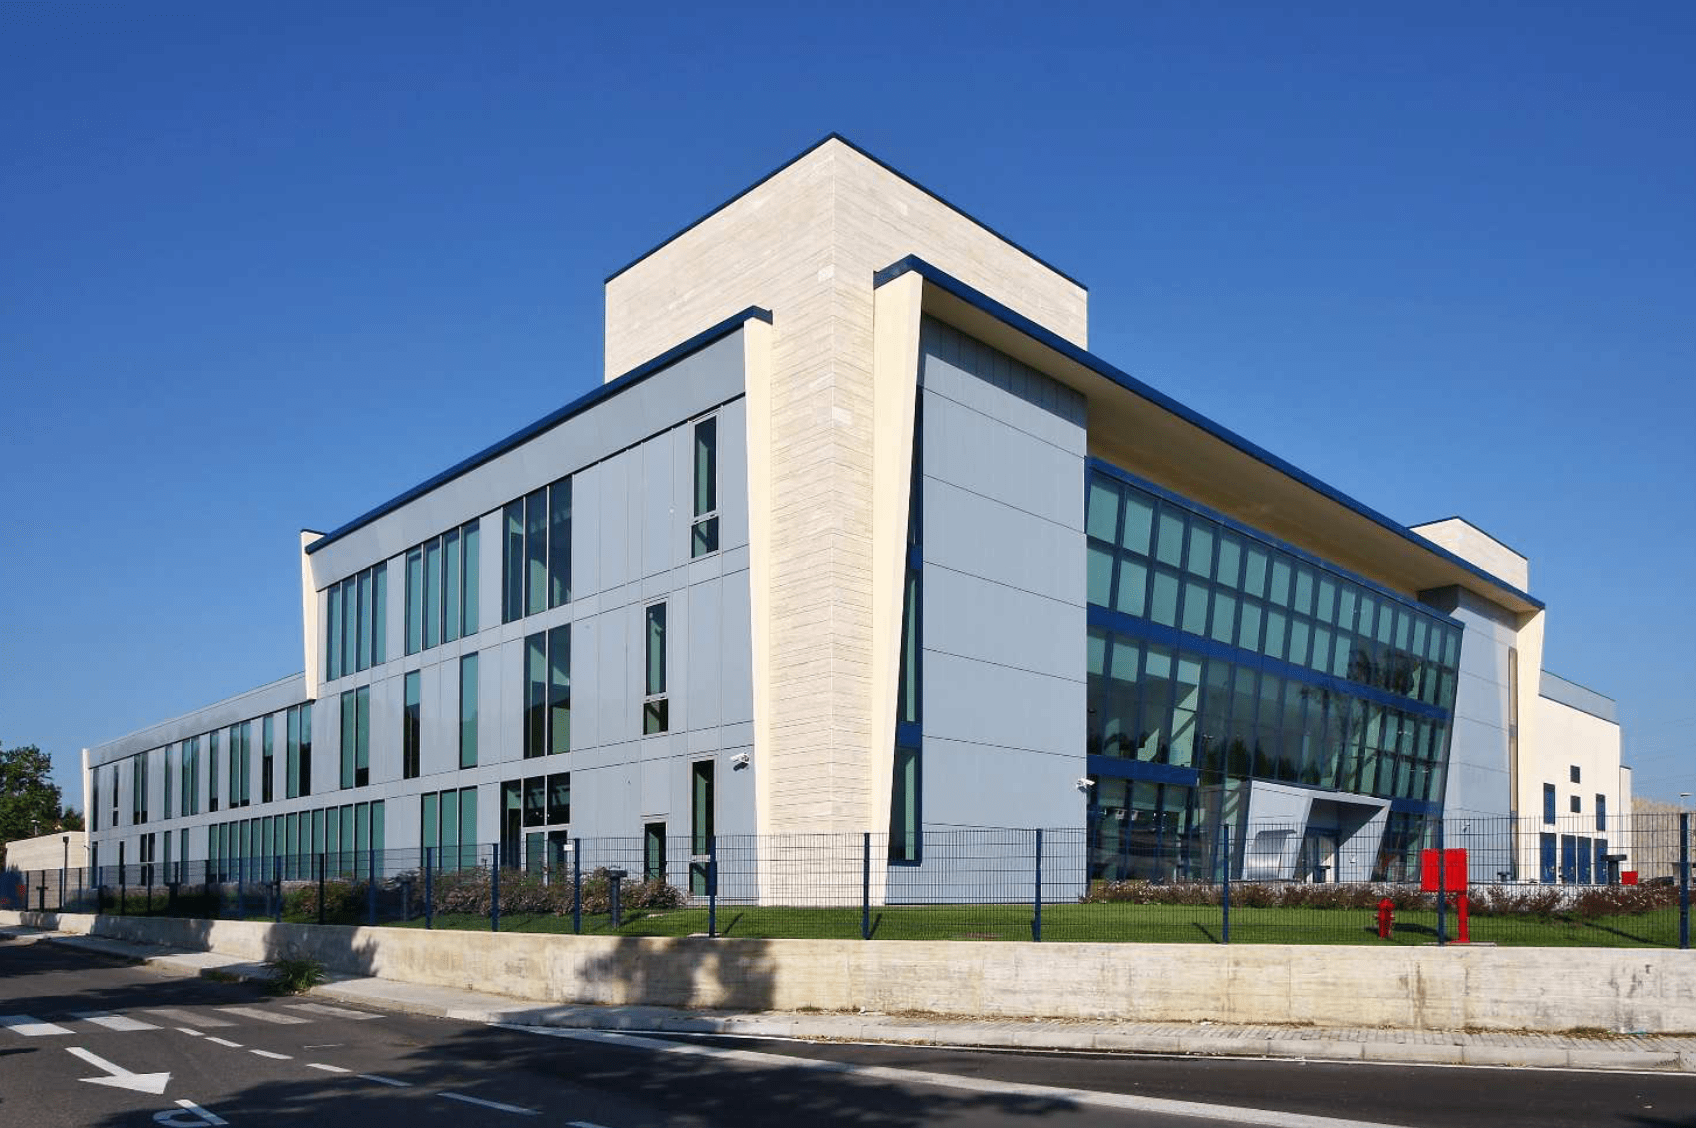
\includegraphics[width=.49\linewidth]{edificio_cnao.jpg}}\hfill
		\subfloat[Una delle sale di trattamento del CNAO. Il fascio è in grado di raggiungere il paziente sia dall'alto che da sinistra \cite{asimmetrie_curareCLP}.]{\label{fig:sala_cnao}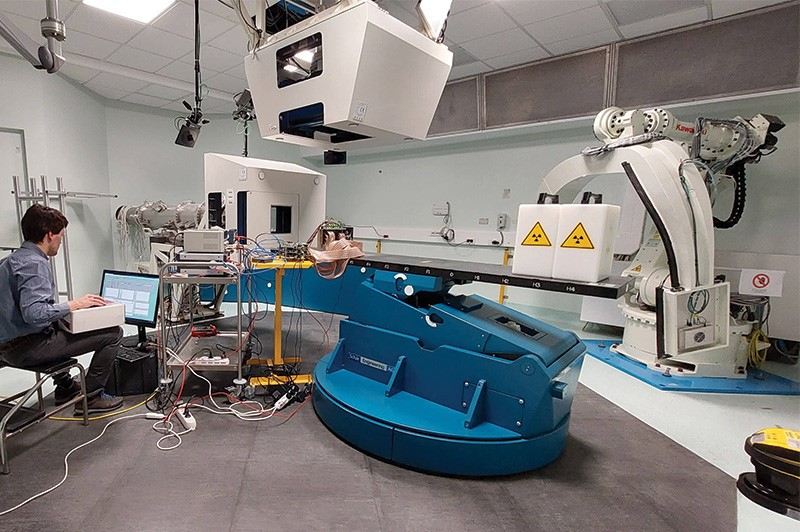
\includegraphics[width=.49\linewidth]{sala_cnao.jpg}}\par 
		\subfloat[Il sincrotrone del CNAO, situato in un bunker di $1600\mbox{ m}^2$ isolato dal resto della struttura e dotato di spesse pareti in cemento armato \cite{cnao6}.]{\label{fig:sincrotrone_cnao}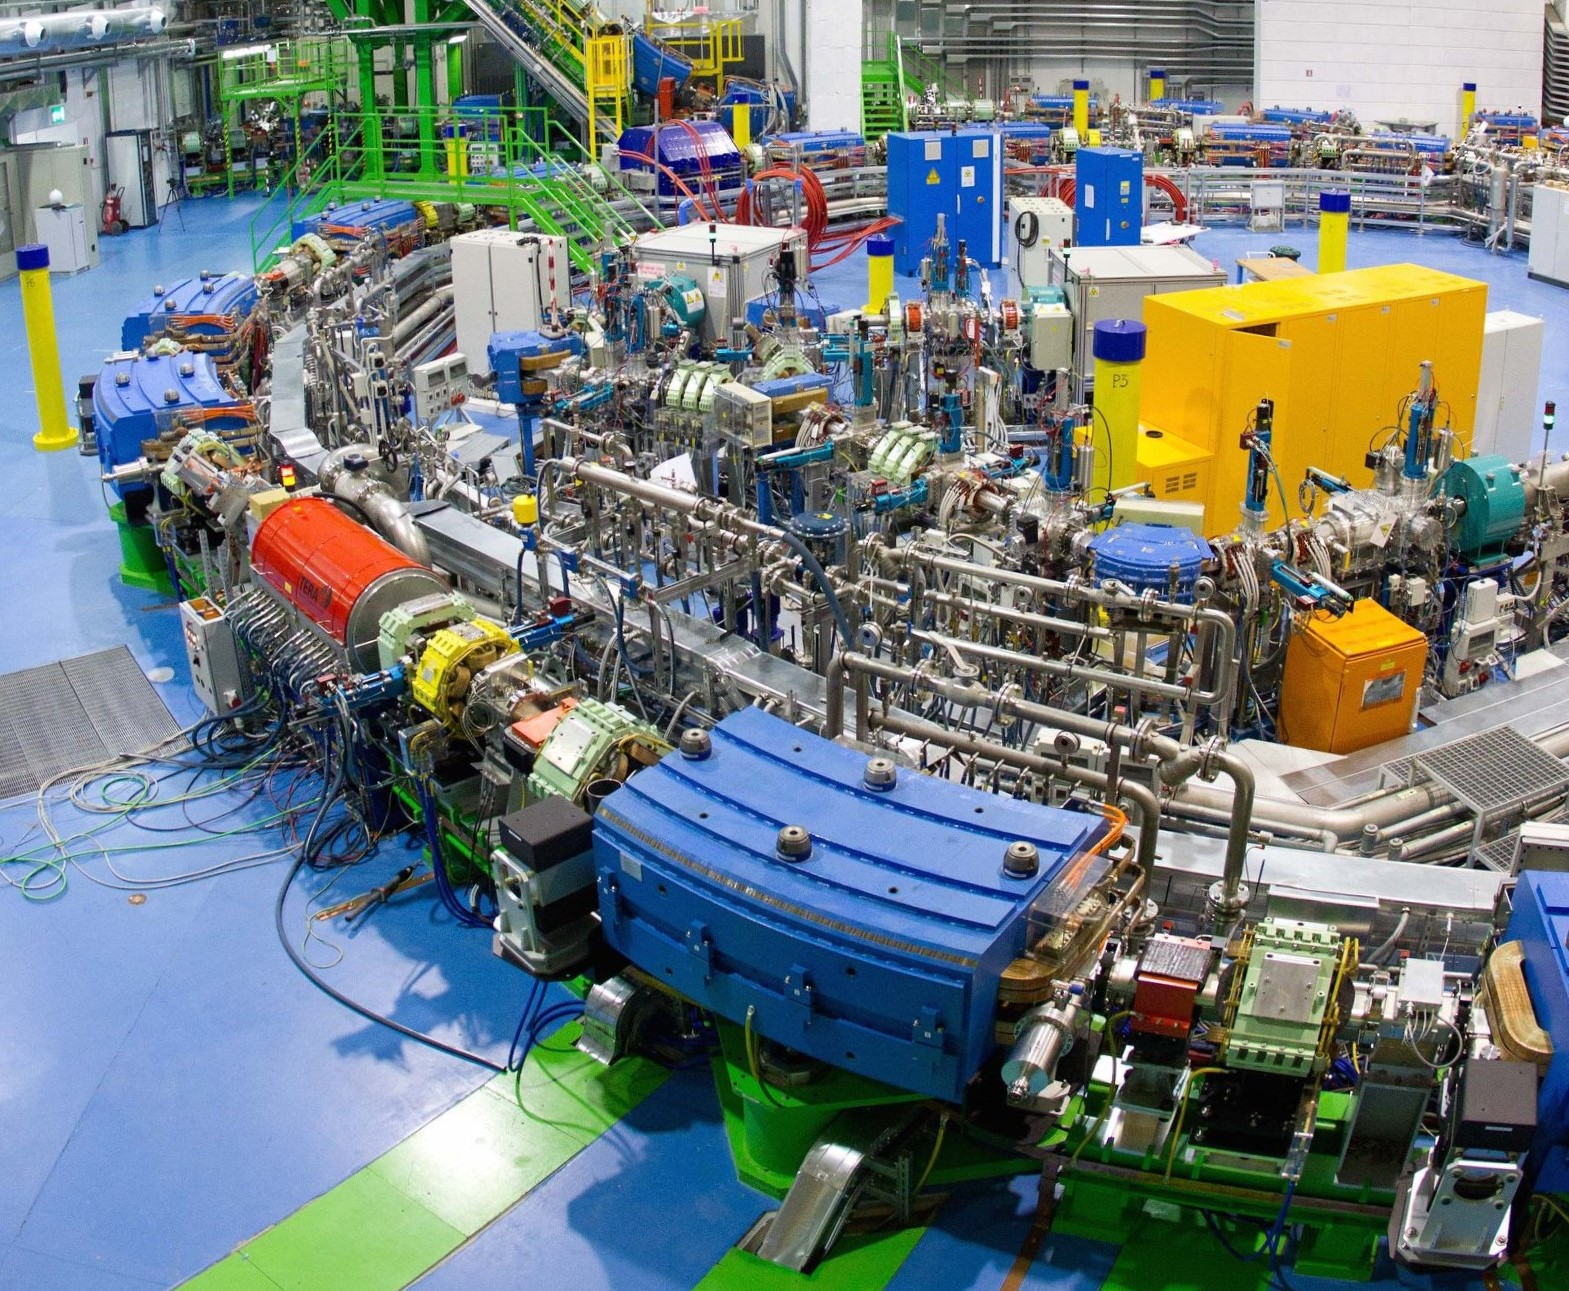
\includegraphics[width=.49\linewidth]{sincrotrone_cnao.jpg}}
		\caption{Immagini relative al CNAO di Pavia.}
		\label{fig:cnao}
	\end{figure}
	Gli attuali obiettivi del CNAO non sono solo quelli di arrivare a trattare circa $700$ pazienti all’anno, ma anche di diventare l’unico centro di adroterapia al mondo a disporre di protoni, ioni carbonio (e altre specie ioniche) e neutroni attraverso la Boron Neutron Capture Therapy (BNCT)\footnote{Nella BNCT si iniettano farmaci arricchiti con \ce{^{10}B} nel sito tumorale; quest'ultimo viene irradiato con neutroni di bassa energia in modo da sfruttare la loro reazione nucleare con i nuclei di \ce{^{10}B}, che produce nuclei radioattivi il cui decadimento libera radiazioni ionizzanti ad alta energia \cite{asimmetrie_curareCLP}.} \cite{cnao3,cnao4}.
	\begin{figure}[H]
		\centering
		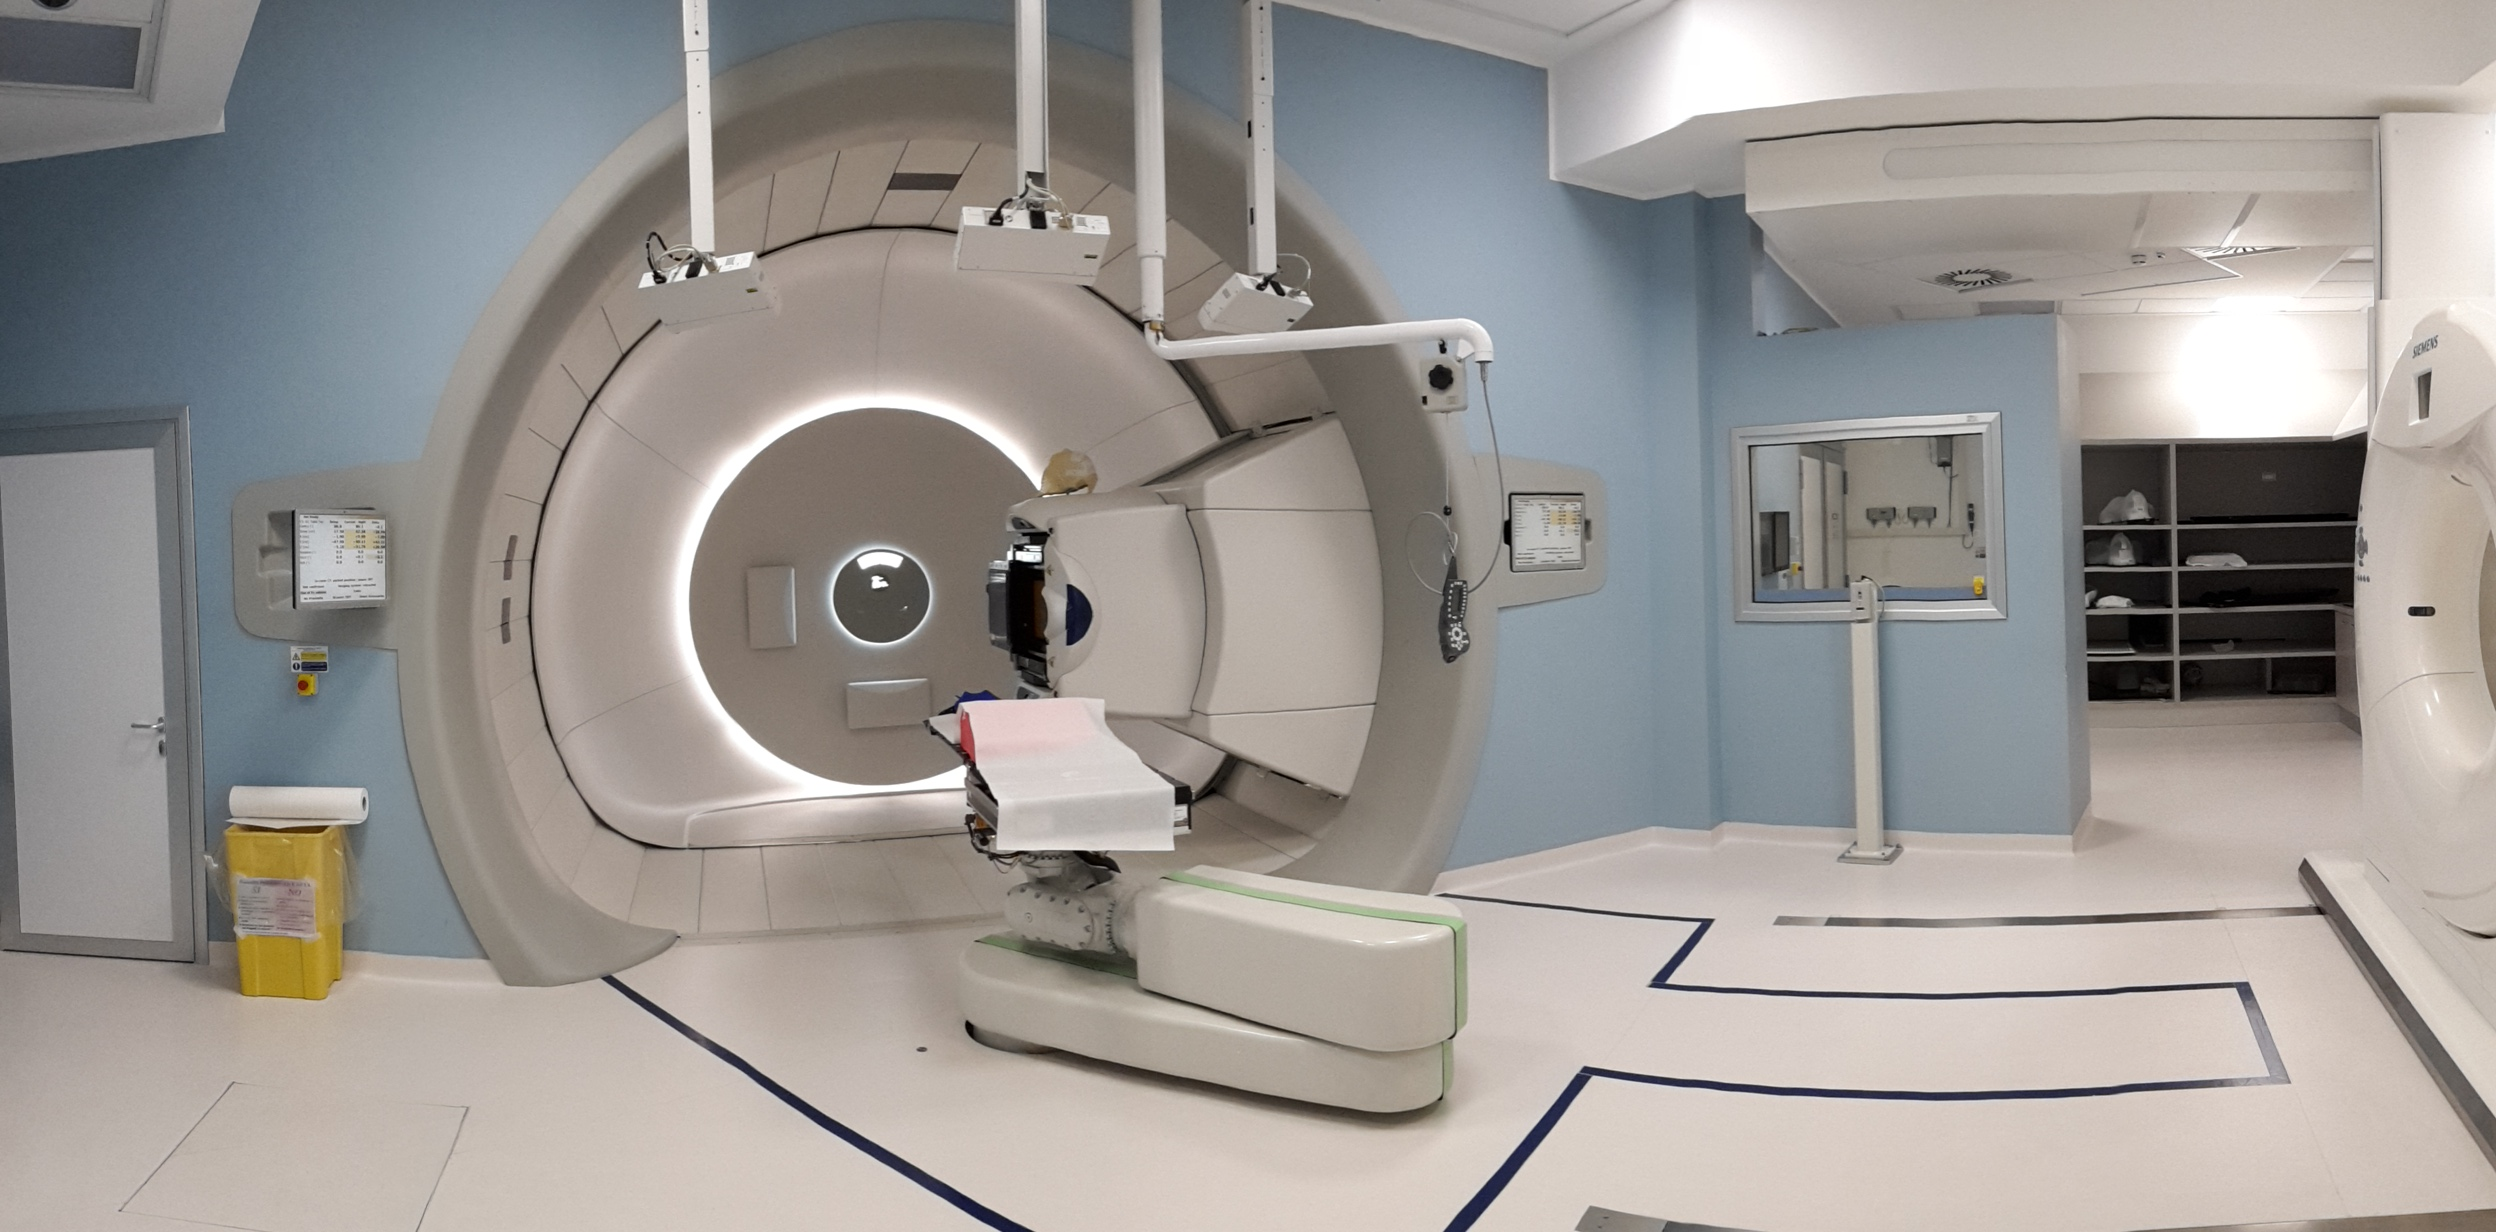
\includegraphics[width=0.9\linewidth]{gantry.jpg}
		\caption{Sistema gantry ``Blu'' del Centro di Protonterapia di Trento \cite{protonterapia_wiki}.}
		\label{fig:gantry}
	\end{figure}
	Il centro adroterapico italiano più recente è il Proton Therapy Center (PTC) di Trento, la cui attività clinica ha avuto inizio nell'ottobre del $2014$ \cite{trento_pt}. Il PTC, che è una delle unità operative del Dipartimento di Oncologia dell'Ospedale di Trento, utilizza solo fasci di protoni accelerati da un ciclotrone a un'energia di $70$--$226 \mbox{ MeV}$ \cite{FRACCHIOLLA2019215}. Uno dei punti di forza del PTC è la sua capacità di erogare protoni per mezzo di sistemi rotanti (gantry, \hyperref[fig:gantry]{Fig. 1.6}), garantendo un trattamento del paziente full-body a $360^\circ$ necessario per patologie come tumori cerebrali e della base cranica, del distretto cervico-cefalico, della colonna vertebrale, sarcomi dei tessuti molli e tumori pediatrici \cite{trento_servSan}. Inoltre, il centro adroterapico trentino è il primo in Italia capace di erogare un fascio di protoni in modalità attiva; quest'ultima, a differenza delle modalità uniforme e passiva, utilizza campi magnetici per deviare il percorso di ciascun fascio protonico verso la posizione che deve colpire, determinata subito prima che la dose venga erogata \cite{LILT,McGowan2013-pl}. Il PTC possiede due linee protoniche dedicate ai trattamenti clinici dotate di gantry e una linea fissa utilizzata per attività sperimentali di ricerca e sviluppo (R\&D). Le attività di R\&D non sono legate esclusivamente alla protonterapia ma anche a contesti lontani dall'ambito medico, per esempio appartenenti all'ambito aerospaziale (come la radioprotezione) ed elettronico (come lo studio di componenti elettroniche radioresistenti) o legati all'analisi dei materiali e lo sviluppo di rivelatori \cite{trento_pt2}.
	
	\subsubsection{Tecniche e R\&D nel percorso radioterapico}
	Nei moderni centri radio e adroterapici, prima di ogni trattamento, i pazienti compiono un attento percorso di pianificazione del trattamento (TP, Treatment Planning) che include numerosi passaggi fondamentali. Uno di questi è lo studio della topologia del volume tumorale, che avviene tramite tecniche di imaging diagnostico morfologico e funzionale come TAC (Tomografia Assiale Computerizzata), RMN (Risonanza Magnetica Nucleare), PET (Tomografia a Emissione di Positroni) e SPECT (Tomografia a Emissione di Singolo Fotone), metodi che con lo sviluppo tecnologico forniscono mappe tridimensionali dei tessuti del corpo umano sempre più dettagliate. Un altro compito del TP è anche quello di pianificare la dose totale a cui sottoporre il paziente e il suo frazionamento; ad esempio, al CNAO i trattamenti con fasci di protoni e di ioni carbonio richiedono in media rispettivamente $35$ e $16$ sedute \cite{cnao7}.
	
	Attualmente, un importante obiettivo della R\&D adroterapica è migliorare la sensibilità degli strumenti utilizzati per il rilascio di dose nel paziente. Un dosaggio più preciso consentirebbe interventi mirati alle cellule tumorali e un migliore risparmio dei tessuti sani; inoltre, una strumentazione di rilascio adattiva risulterebbe utile a seguire ogni minimo movimento (anche respiratorio) del paziente, sebbene quest'ultimo venga già immobilizzato da opportune fasce durante il trattamento. Per tali motivi, è fondamentale implementare l'efficacia dei rivelatori in grado di misurare l'irraggiamento dei fasci adronici e sviluppare micro e nano-dosimetri per consentire un minuzioso rilascio di dose.
	
	La R\&D adroterapica si occupa anche di migliorare la comprensione degli effetti delle radiazioni sul corpo umano. Ciò avviene attraverso la teorizzazione di modelli matematici che legano la sopravvivenza cellulare con il tipo di irraggiamento adroterapico ricevuto e lo studio di tecniche di imaging ricostruttivo in grado di misurare i cambiamenti anatomici che il tumore e gli organi limitrofi possono subire anche in breve tempo.
	
	I programmi di R\&D sopra elencati richiedono il lavoro congiunto di oncologi, radiologi e fisici che uniscono imprescindibili competenze in radiobiologia, elettronica, fisica dei materiali e computing. In particolare, al giorno d'oggi si sfruttano copiosamente sistemi di calcolo avanzati, metodi di intelligenza artificiale (come algoritmi di deep learning e machine learning) e simulazioni Montecarlo in grado di compiere analisi predittive e adattive, divenute ormai fondamentali nel contesto applicativo delle scienze omiche \cite{asimmetrie_curareCLP,asimmetrie_DLAS,asimmetrie_curareGD}.
	
	\section{Parametri fisici ed effetti biologici della radiazione}
	Come descritto nella \hyperref[sec:1.1]{Sez. 1.1}, le cellule tumorali generano un disequilibrio dell'omeostasi dell'organismo umano poiché, a differenza delle cellule sane, sfuggono ai meccanismi di controllo che limitano la loro proliferazione (una regolazione che avviene automaticamente in condizioni normali). Infatti, molte cellule malate non sono capaci di arrestare il ciclo cellulare nei punti di controllo,\footnote{I punti di controllo sono stadi del ciclo cellulare in cui quest'ultimo subisce automaticamente un arresto, in attesa che arrivi un segnale che permetta la sua prosecuzione.} nemmeno quando sono assenti i fattori di crescita\footnote{I fattori di crescita sono proteine che stimolano la divisione di alcune cellule. Una loro assenza inibirebbe la divisione cellulare.} \cite{campbell3anno}.
	
	Le alterazioni del ciclo cellulare sono generalmente causate da disfunzioni dell'espressione genica (\hyperref[fig:mutazioni_genetiche]{Fig. 1.7}), che è il processo con cui l'informazione contenuta nei geni fluisce alle proteine (le macromolecole funzionali del nostro corpo) tramite meccanismi di trascrizione e traduzione del DNA. I geni modificati capaci di generare cellule tumorali sono denominati oncogeni. Di solito le cellule sane acquisiscono un oncogene a partire da una mutazione di uno dei propri geni, chiamato proto-oncogene. Il cromosoma degli esseri umani contiene naturalmente proto-oncogeni, molti dei quali (in condizioni ordinarie) svolgono ruoli essenziali per il ciclo cellulare, come codificare per i fattori di crescita; tuttavia, tali proto-oncogeni possono convertire in oncogeni nelle modalità descritte nella \hyperref[fig:oncogene]{Fig. 1.7a}. Oltre ai proto-oncogeni, che stimolano la divisione cellulare, esistono gli oncosoppressori, geni che codificano per proteine che inibiscono la proliferazione cellulare incontrollata. Per questo motivo, mutazioni che riducono le attività delle proteine codificate dai geni oncosoppressori possono portare all'insorgenza di un tumore (\hyperref[fig:oncosoppressore]{Fig. 1.7b}).
	\begin{figure}[H]
		\centering
		\begin{subfigure}[b]{0.85\textwidth}
			\centering
			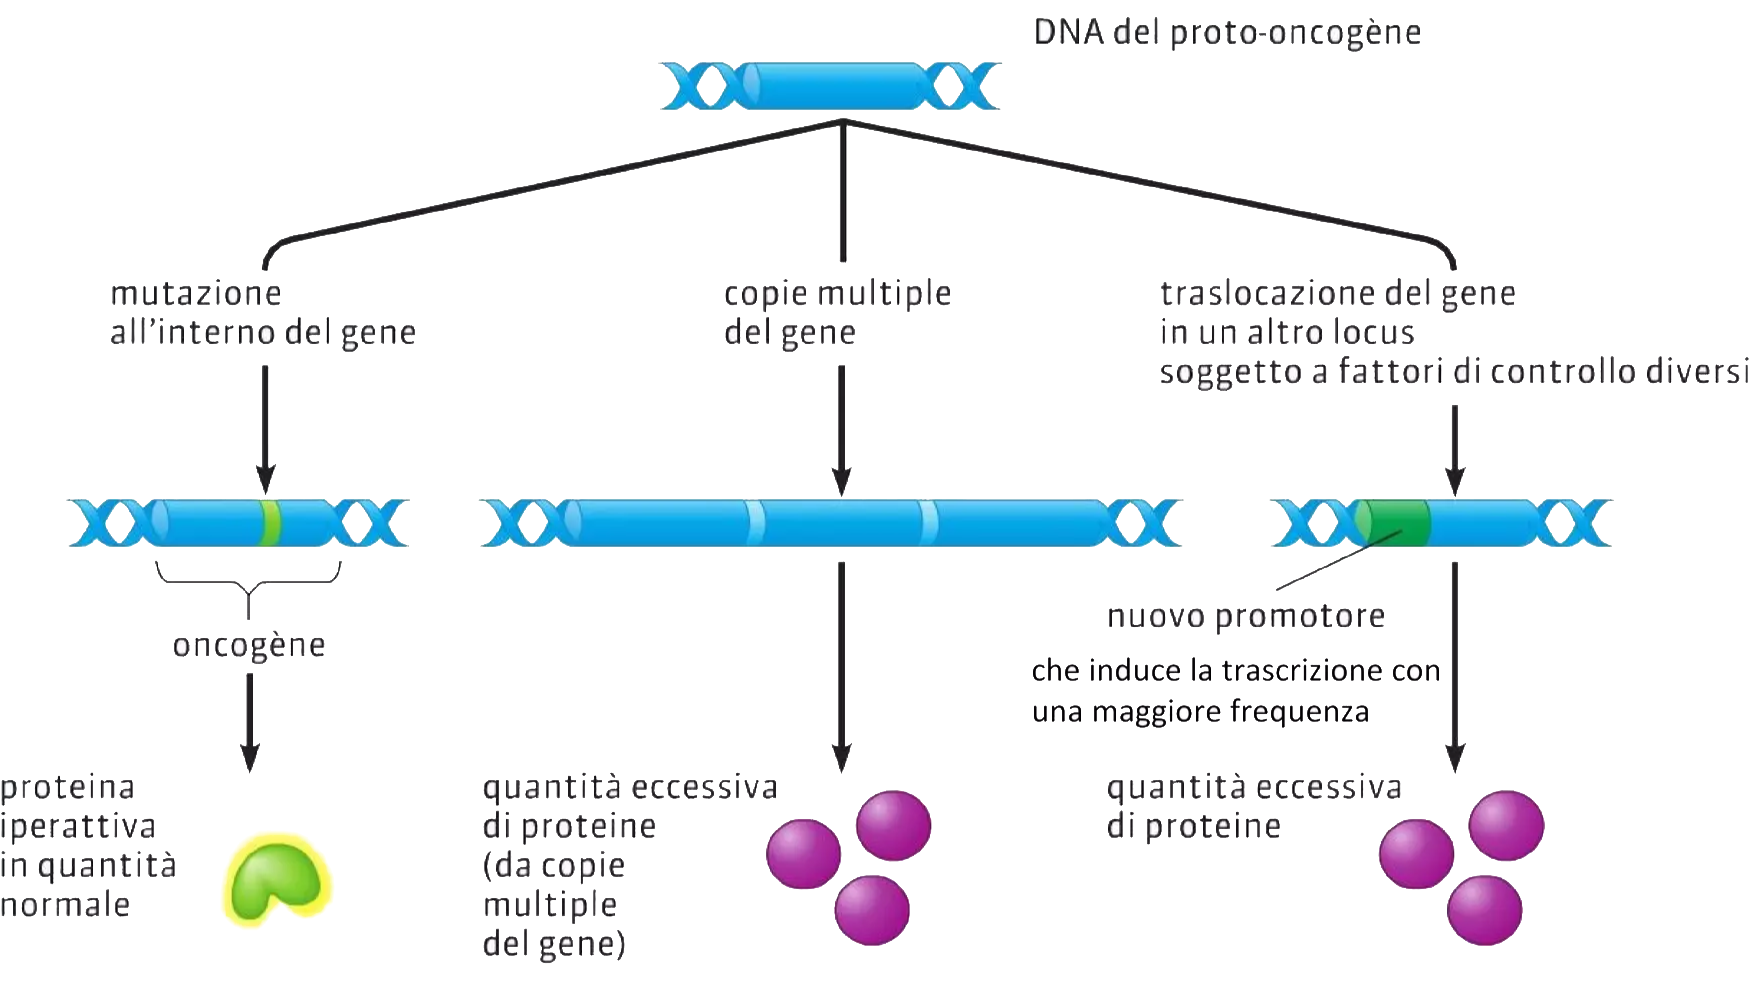
\includegraphics[width=\textwidth, scale=0.5]{oncogene.png}
			\caption{Schematizzazione dei tre modi con cui un proto-oncogene codificante per fattori di controllo può mutare in un oncogene.}
			\label{fig:oncogene}
		\end{subfigure}
		\par
		\begin{subfigure}[b]{0.85\textwidth}
			\centering
			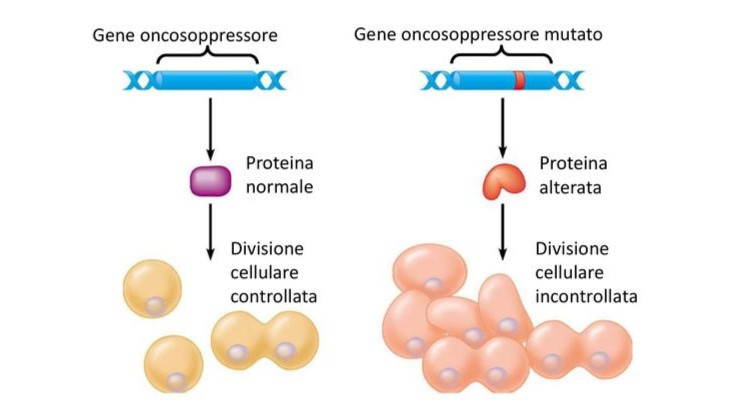
\includegraphics[width=\textwidth, scale=0.5]{oncosoppressore.jpg}
			\caption{Effetto della mutazione di un gene oncosoppressore.}
			\label{fig:oncosoppressore}
		\end{subfigure}
		\caption{Esempi di mutazioni subite da geni che controllano la divisione cellulare \cite{campbell2anno}.}
		\label{fig:mutazioni_genetiche}
	\end{figure}
	Il fatto che le neoplasie siano originate da danni genetici è un'ipotesi ampiamente acclarata, che si basa su osservazioni come il ritrovamento di cromosomi danneggiati in cellule cancerose, il riconoscimento di una predisposizione ereditaria al cancro e il rapporto fra suscettibilità al cancro e incapacità delle cellule a riparare il DNA danneggiato \cite{treccani_oncogeni}. Per esempio, si pensi che le mutazioni di due noti geni \textit{ras} (proto-oncogene) e \textit{p53} (oncosoppressore) sono rilevate rispettivamente nel $30\%$ e in più del $50\%$ dei casi di cancro umano \cite{campbell3anno}.
	
	\subsection{Danni biologici delle radiazioni ionizzanti}
	La radioterapia e l'adroterapia, come descritto in \hyperref[sec:1.2]{Sez. 1.2}, sfruttano la radiazione ionizzante per danneggiare i tessuti biologici cancerosi al fine di causare la morte delle cellule malate che li costituiscono. La radiazione ionizzante produce vari effetti sui tessuti biologici che dipendono da svariati fattori, tra cui l'energia del fascio incidente, la sua composizione e le caratteristiche del tessuto irradiato. Per comprendere i danni biologici che la radiazione provoca sui tessuti cancerosi, è opportuno analizzare ciò che accade a livello cellulare.
	
	Per le cellule tumorali si parla di morte riproduttiva nel momento in cui la cellula perde la sua capacità di riprodursi indefinitamente. Per sconfiggere una neoplasia non occorre eliminare tutte le cellule tumorali, piuttosto è necessario impedire alla cellula di riprodursi per mitosi (o meiosi se si tratta di una cellula deputata alla riproduzione \cite{campbell2anno}) mediante la distruzione del DNA contenuto nel suo nucleo. Per uccidere il DNA cellulare tramite radiazione ionizzante vi sono due modi, diretto e indiretto, descritti nei paragrafi seguenti.
	
	\subsubsection{Danno diretto}\label{par:danno_diretto}
	Prima di analizzare il danno diretto che la radiazione può arrecare al DNA, è opportuno descrivere la struttura e le funzioni di quest'ultimo. Il DNA (acido desossiribonucleico) è un polimero costituito da monomeri chiamati nucleotidi, molecole a loro volta composte da una base azotata, uno zucchero e un gruppo fosfato (si veda \hyperref[fig:nucleotide]{Fig. 1.8}). Esistono quattro tipi di nucleotidi, la cui specificità è data dal tipo di base azotata: adenina (A), citosina (C), timina (T) o guanina (G). Oltre al DNA esiste anche l'RNA (acido ribonucleico), un acido nucleico fondamentale per la biosintesi delle proteine. Nonostante DNA e RNA siano entrambi costituiti da una lunga catena nucleotidica, presentano varie differenze strutturali e funzionali:
	\begin{itemize}
		\item il DNA possiede una struttura a doppia elica (caratterizzata dal diametro costante di $2\mbox{ nm}$ \cite{campbell3anno}) costituita da due catene nucleotidiche antiparallele (unite tramite legami idrogeno tra A e T oppure tra C e G), mente l'RNA è formato da una singola elica in cui T viene sostituita dall'uracile (U) (\hyperref[fig:dna_structure]{Fig. 1.9});
		\item lo zucchero del DNA (desossiribosio) possiede un atomo di ossigeno in meno rispetto a quello dell'RNA (ribosio);
		\item nelle cellule eucariote, il DNA è collocato nel nucleo mentre l'RNA si trova sia nel nucleo che nel citoplasma;
		\item il DNA è depositario dell'informazione genetica mentre l'RNA è l'intermediario tra il DNA e la sintesi delle proteine.
	\end{itemize}
	\begin{figure}[H]
		\centering
		\includegraphics[width=0.5\linewidth]{nucleotide.pdf}
		\caption{Nucleotide formato a sinistra da un gruppo fosfato contenente un atomo di fosforo \ce{P} (che determina il carattere acido degli acidi nucleici), al centro da uno zucchero (desossiribosio) formato da cinque atomi di carbonio e in alto a destra da una base azotata contenente un gruppo \ce{\bond{-}NH} (che conferisce loro un carattere basico) legata con lo zucchero per mezzo di un legame glicosidico \cite{nucleotidi_wiki}.}
		\label{fig:nucleotide}
	\end{figure}
	La scoperta delle strutture degli acidi nucleici DNA e RNA (\hyperref[fig:dna_structure]{Fig. 1.9}) viene attribuita agli scienziati James D. Watson ($1928$--), Francis H. C.Crick ($1916$--$2004$) e Maurice H. F. Wilkins ($1916$--$2004$), che per il loro contributo alla biologia molecolare ricevettero il premio Nobel per la fisiologia o medicina nel $1958$. In realtà la prima immagine cristallografica del DNA fu quella della chimica Rosalind E. Franklin ($1920$--$1958$), anche se per molto tempo non gli fu riconosciuta la paternità della scoperta. Purtroppo la sua morte precoce non le consentì nemmeno di essere candidata al premio Nobel \cite{campbell3anno}.
	\begin{figure}[H]
		\centering
		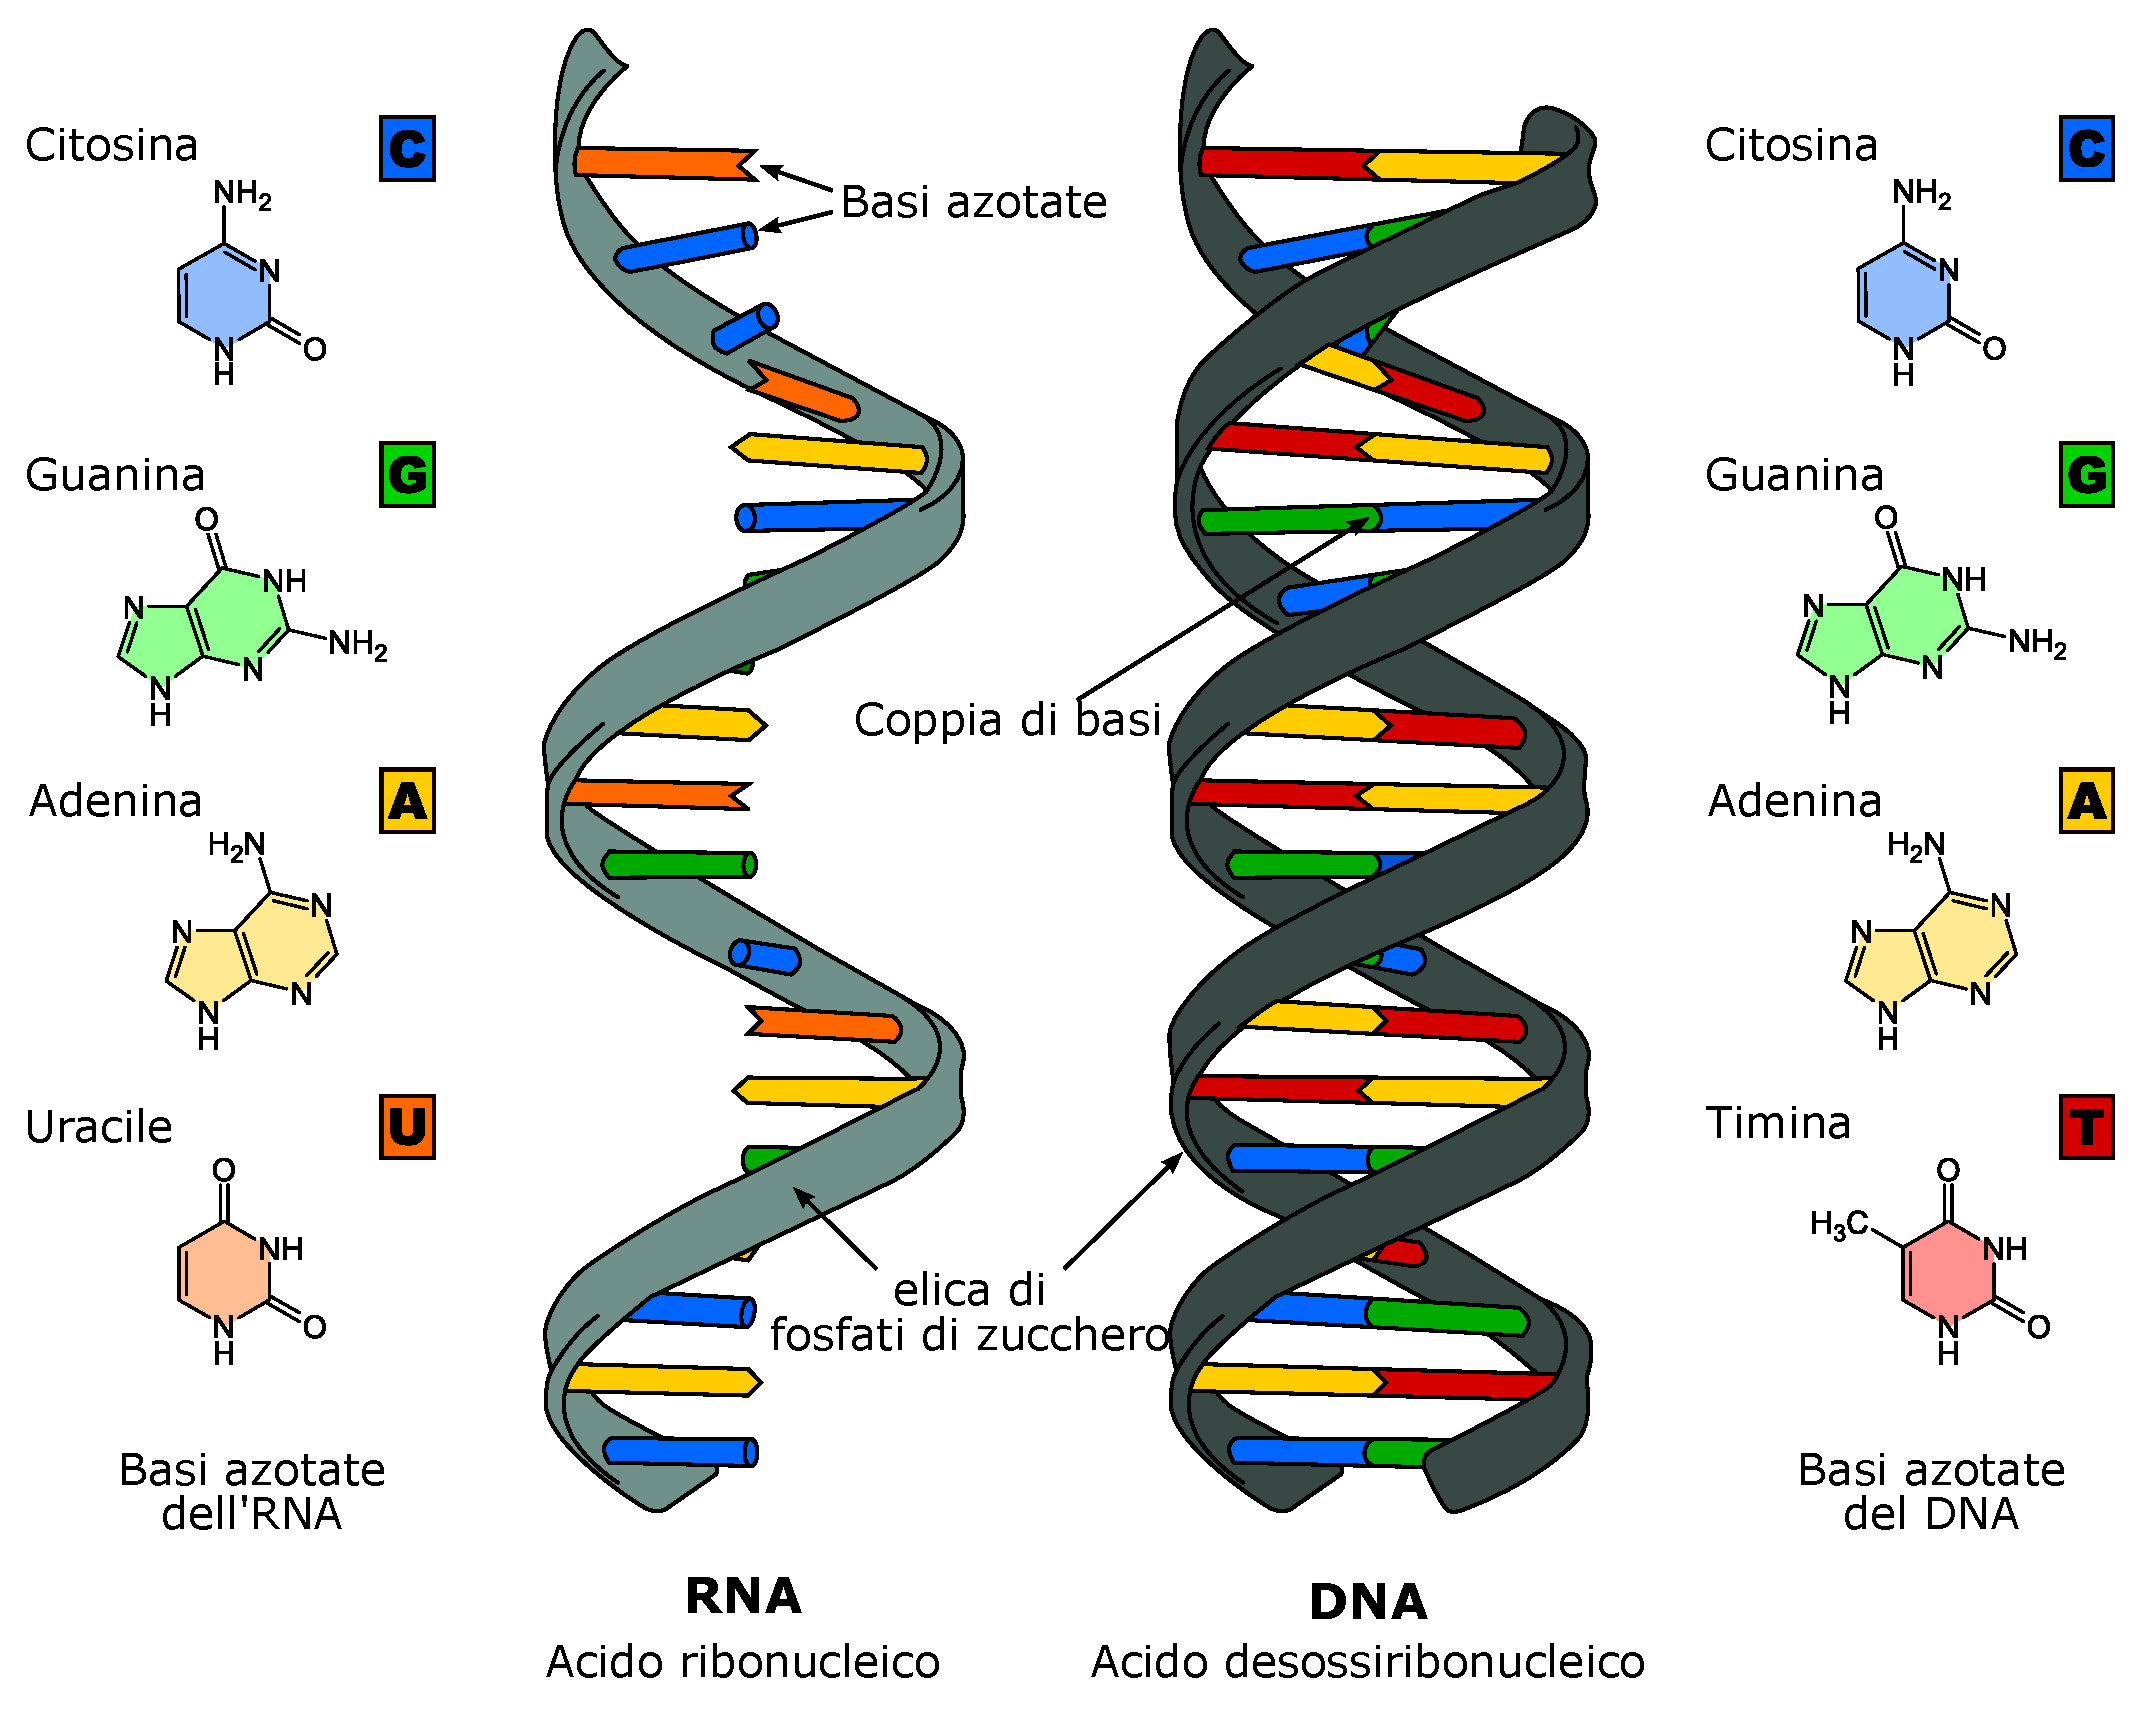
\includegraphics[width=0.9\linewidth]{dna_structure.pdf}
		\caption{Struttura a singola elica dell'RNA e a doppia elica del DNA con relativi accoppiamenti delle basi azotate \cite{nucleic_acids_wiki}.}
		\label{fig:dna_structure}
	\end{figure}
	Come accennato in precedenza, le funzioni del DNA sono quelle di regolare la riproduzione delle cellule (mediante la sua duplicazione che favorisce la trasmissione delle informazioni ereditarie) e di controllare l'espressione genica. In particolare, il dogma centrale della biologia molecolare (proposto nel $1956$ dallo stesso Francis Crick \cite{campbell3anno}) prevede che le fasi principali della sintesi proteica siano la trascrizione e la traduzione, illustrate in \hyperref[fig:dna_rna]{Fig. 1.10}. Durante la trascrizione si genera un filamento di mRNA (RNA messaggero) le cui basi azotate sono complementari a quelle della molecola di DNA che è utilizzata come stampo (con l'U al posto della T). Durante la traduzione avviene un ``cambiamento di linguaggio'': l'informazione genica contenuta nel DNA (per mezzo dell'mRNA, dell'tRNA (RNA di trasporto) e dei ribosomi) viene tradotta da una sequenza di nucleotidi in una sequenza di amminoacidi, i ``mattoni'' che costituiscono le proteine; nello specifico, ad ogni tripletta di basi azotate (denominata codone) corrisponde un amminoacido (la totalità delle $4^3=64$ combinazioni possibili consente di codificare per tutti i $20$ amminoacidi esistenti in natura). Eventuali variazioni della sequenza nucleotidica (come la sostituzione, l'inserzione o la delezione di una base azotata) generano le mutazioni che, in mancanza dei meccanismi di controllo cellulare, sono la causa di molti disturbi e malattie ereditarie \cite{campbell3anno}.
	\begin{figure}[H]
		\centering
		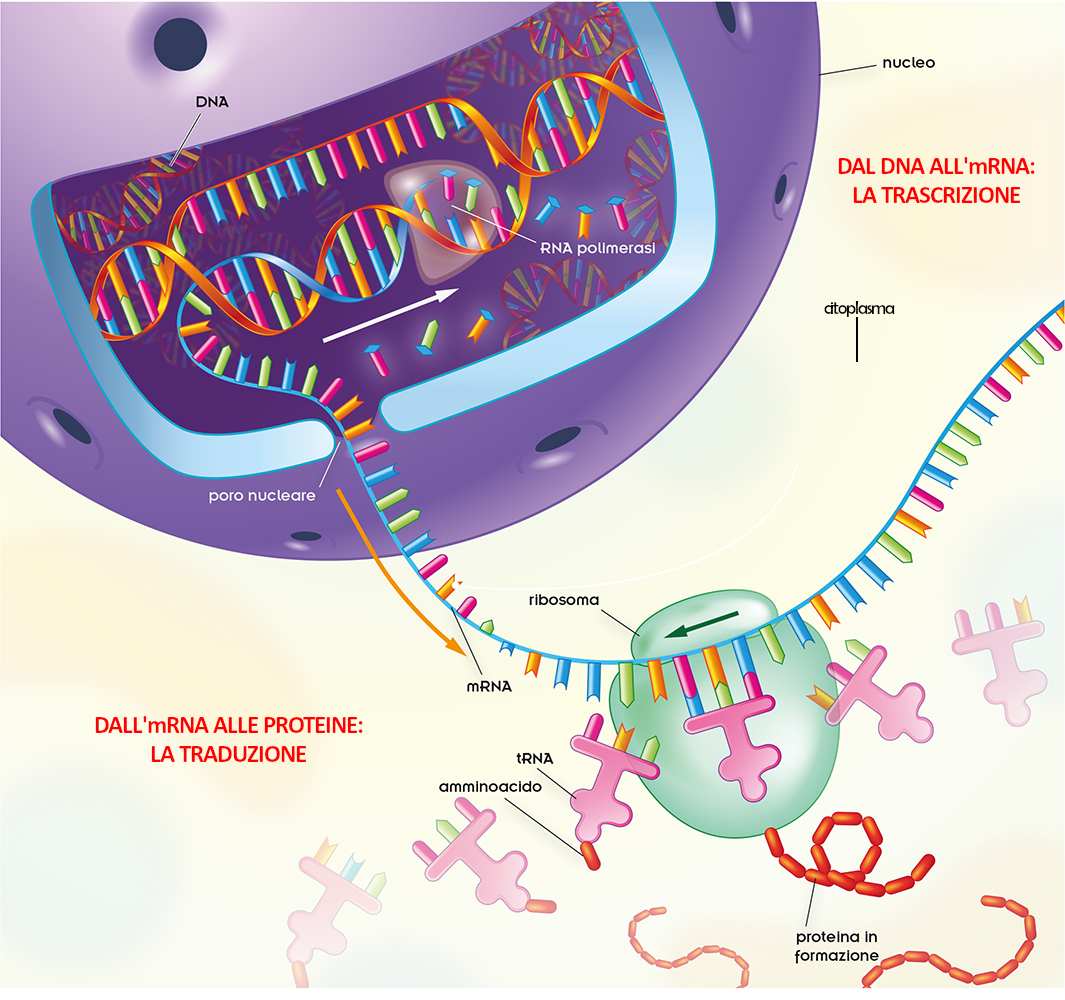
\includegraphics[width=0.85\linewidth]{dna_rna.jpg}
		\caption{Meccanismi di trascrizione e traduzione grazie ai quali il genotipo (l'insieme delle informazioni ereditarie di un organismo) controlla il fenotipo (le caratteristiche fisiche di un organismo) \cite{hub_scuola,campbell3anno}.}
		\label{fig:dna_rna}
	\end{figure}
	Come già anticipato, il DNA è localizzato nel nucleo della cellula\footnote{In realtà esiste il DNA mitocondriale, un particolare tipo di DNA che contiene informazioni genetiche ereditato solo per linea materna \cite{campbell2anno}, che è situato all'interno dei mitocondri, organuli cellulari in cui avviene la respirazione cellulare.} ed è legato a particolari proteine che formano una struttura fibrosa chiamata cromatina, che al momento della duplicazione cellulare si addensa formando i cromosomi. Dalle considerazioni precedenti, riassunte nella \hyperref[fig:cell]{Fig. 1.11}, si comprende che il DNA occupa solo una minima parte della cellula: solamente il $2$--$3\%$ del volume cellulare è occupato da DNA. Per questo motivo, arrecare danni diretti al DNA da parte di radiazione ionizzante è un evento piuttosto raro, ma non trascurabile.
	\begin{figure}[H]
		\centering
		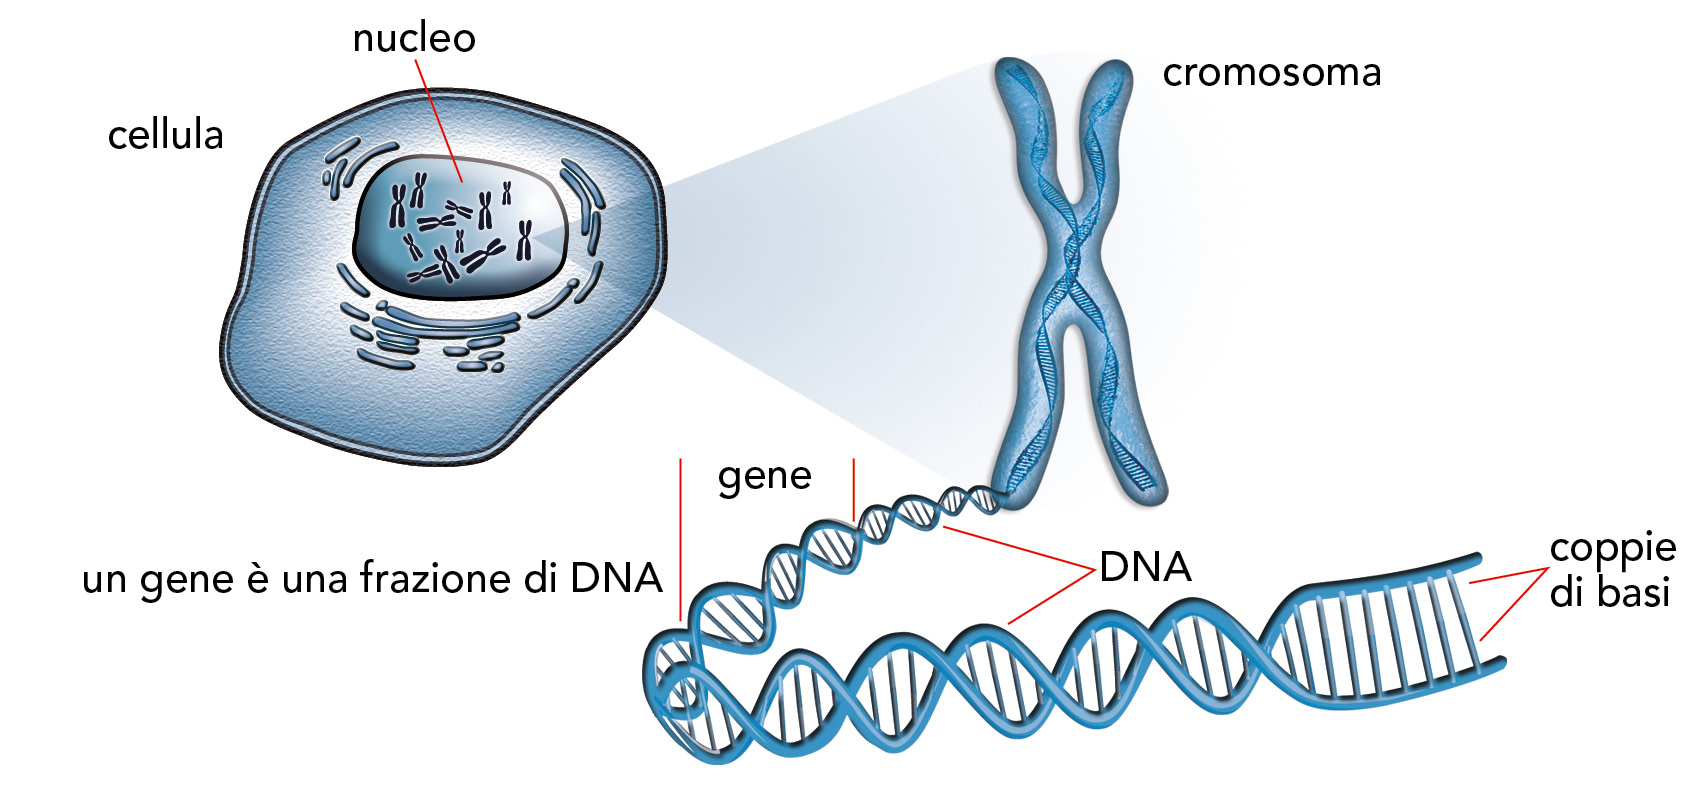
\includegraphics[width=0.9\linewidth]{cell.jpg}
		\caption{Particolari della struttura della cellula eucariote umana. Si noti che ogni gene è costituito da centinaia o migliaia di nucleotidi \cite{dbook}.}
		\label{fig:cell}
	\end{figure}
	Quando la radiazione ionizzante colpisce direttamente il DNA, quest'ultimo può subire danni differenti la cui distribuzione dipende dal tipo di radiazione e dall'energia del fascio incidente. In generale, è possibile suddividere i danni in Single Strand Break (SSB) e Double Strand Breaks (DSB): nei SSB si genera la rottura di un solo filamento nucleotidico della doppia elica del DNA, mentre nei DSB si ha un danneggiamento in entrambe le catene nucleotidiche, come rappresentato in \hyperref[fig:danni_dna]{Fig. 1.12}. Grazie al meccanismo di correzione di bozze, enzimi specifici come DNA polimerasi, DNA ligasi e nucleasi riconoscono i nucleotidi fuori posto e li sostituiscono (mediante un meccanismo chiamato ``riparazione delle anomalie di appaiamento'') prima che possano portare a mutazioni genetiche.\footnote{Ricerche hanno dimostrato che difetti ereditari agli enzimi sopra citati sono associati a una forma di cancro al colon, in quanto gli errori che portano al cancro si accumulano nel DNA più velocemente \cite{campbell2anno}.} L'efficacia dei metodi di riparazione cellulare dipende dalla complessità del danno iniziale: nei SSB la catena danneggiata viene sostituita dagli enzimi osservando le informazioni della catena integra (sfruttando la complementarietà delle basi azotate), mentre nei DSB si hanno danni che non consentono una ricostruzione della doppia elica; infatti, solo in quest'ultimo caso la cellula potrebbe andare incontro o a morte cellulare (danno deterministico voluto in radio e adroterapia per ottenere l'eliminazione di cellule tumorali) o a carcinogenesi (danno stocastico da limitare in radio e adroterapia, la cui insorgenza è legata alle conseguenze a lungo termine dell'esposizione alla radiazione), perdendo in ambo i casi la sua capacità riproduttiva \cite{unipv_conference}.
	\begin{figure}[H]
		\centering
		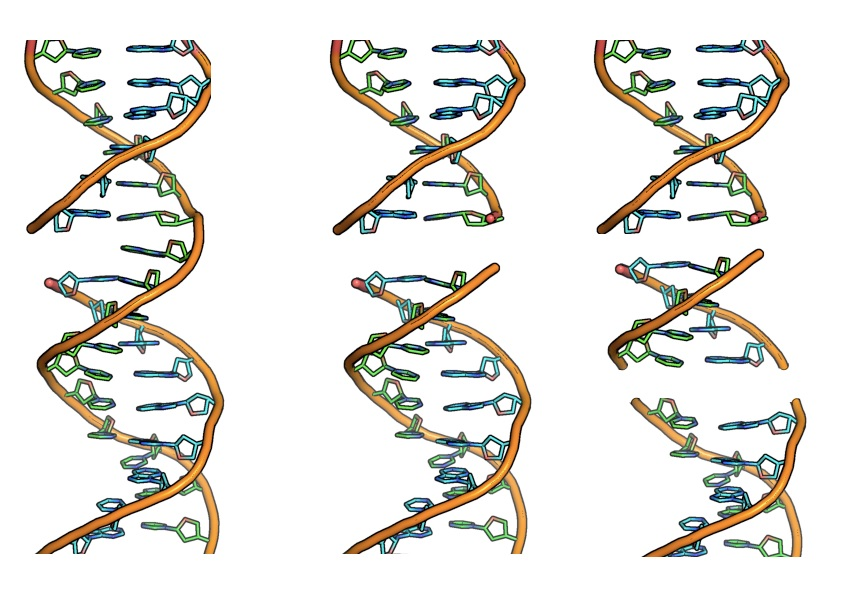
\includegraphics[width=0.9\linewidth]{danni_dna.jpg}
		\caption{Schematizzazione dei SSB (a sinistra), dei DSB (al centro) e di cluster di DSB (a destra) \cite{unipv_conference}.}
		\label{fig:danni_dna}
	\end{figure}
	
	\subsubsection{Danno indiretto}\label{par:danno_indiretto}
	Per i motivi esposti nel paragrafo precedente, circa i $2/3$ dei danni cellulari si generano utilizzando radiazione ionizzante che non colpisce direttamente il DNA \cite{dkfz_conference}. Uno dei danni indiretti più frequenti si ha quando la radiazione colpisce l'acqua contenuta nelle cellule cancerose,\footnote{Dato che il corpo umano è costituito per il $75\%$ da acqua, irradiare la cellula equivale, di fatto, a irradiare acqua.} producendo radicali liberi\footnote{I radicali liberi sono atomi neutri o molecole che possiedono un unico elettrone spaiato nel loro orbitale più esterno, caratteristica che è fonte di grande instabilità chimica; ciò rende i radicali liberi particolarmente reattivi e in grado sia di legarsi ad altri radicali sia di sottrarre elettroni a molecole vicine \cite{Silvestroni1996-xz}.} tramite processi di radiolisi\footnote{Per radiolisi chimica si intende la scissione di uno o più legami causata da radiazioni ionizzanti \cite{IUPAC+R05112+2019}.} dell'acqua. La radiolisi dell'acqua consiste in una catena di reazioni chimiche (alcune delle quali riportate di seguito) che producono elettroni, atomi, molecole e ioni che, diffondendo, danneggiano indirettamente il DNA portando alla morte cellulare.
	
	La ionizzazione di una molecola d'acqua (\ce{H2O}) è riassunta nella \hyperref[eq:radiolisi1]{Eq. 1.1}:
	\begin{equation}
		\ce{H2O ->[Radiazione ionizzante] H2O^{+} + e^-}
		\label{eq:radiolisi1}
	\end{equation}
	da cui si producono uno ione positivo \ce{H2O^{+}} e un elettrone \ce{e^-}. Trascorso un certo intervallo di tempo, alcuni elettroni perdono una buona parte della loro energia cinetica (derivata dalla ionizzazione), che rende possibile la cattura elettronica da parte di un'altra molecola d'acqua, con conseguente formazione di uno ione negativo \ce{H2O^{-}}:
	\begin{equation}
		\ce{H2O + e^{-} ->[Cattura elettronica] H2O^{-}}
		\label{eq:radiolisi2}
	\end{equation}
	In seguito, i prodotti delle \hyperref[eq:radiolisi1]{Eq. 1.1} ed \hyperref[eq:radiolisi2]{Eq. 1.2} si dissociano nei seguenti modi:
	\begin{subequations}
		\begin{align}
			\label{eq:dissociazione1}
			\ce{H2O^{+} ->[Dissociazione] H^{+} + OH^{.}}\\
			\label{eq:dissociazione2}
			\ce{H2O^{-} ->[Dissociazione] OH^{-} + H^{.}}
		\end{align}
	\end{subequations}
	i cui prodotti sono gli ioni idrogeno \ce{H^{+}} e ossidrile \ce{OH^{-}} e i radicali liberi ossidrile \ce{OH^{.}} e idrogeno \ce{H^{.}}. Tra le varie reazioni chimiche che possono avvenire successivamente (i cui reagenti sono i prodotti delle \hyperref[eq:dissociazione1]{Eq. 1.3a} ed \hyperref[eq:dissociazione2]{Eq. 1.3b}) si riportano le seguenti:
	\begin{subequations}
		\begin{align}
			\label{eq:prodotto1}
			\ce{H^{.} + OH^{.} &-> H2O}\\
			\label{eq:prodotto2}
			\ce{H^{+} + OH^{-} &-> H2O}\\
			\label{eq:prodotto3}
			\ce{2OH^{.} &-> H2O2}
		\end{align}
	\end{subequations}
	Le \hyperref[eq:prodotto1]{Eq. 1.4a} ed \hyperref[eq:prodotto2]{Eq. 1.4b} sono reazioni innocue in quanto generano molecole d'acqua mentre la \hyperref[eq:prodotto3]{Eq. 1.4c} porta alla formazione di perossido di idrogeno (acqua ossigenata, \ce{H2O2}), una sostanza nociva per la cellula in quanto capace di modificare la struttura e le funzioni delle proteine, di mutare le basi nucleotidiche e di generare SSB nel DNA \cite{ros}. Ciò spiega il motivo per cui i danni indiretti al DNA, per mezzo della catena di radiolisi dell'acqua, possono condurre la cellula alla morte riproduttiva \cite{w3010235}.
	
	Il corpo umano attua una serie di meccanismi di difesa in presenza di \ce{H2O2} e di altre specie chimiche legate all'ossigeno (come i due radicali anione superossido \ce{O2^{-.}} e ossidrile \ce{OH^{.}}), generalmente denominate ROS (Specie Reattive all'Ossigeno). Tali tecniche di difesa si attivano in maniera naturale durante le reazioni di riduzione dell'ossigeno in acqua, da cui i mitocondri cellulari ricavano energia (ATP) per il corpo umano. Il primo meccanismo di difesa è quello di disattivare il radicale \ce{O2^{-.}} tramite l'enzima superossido dismutasi (SOD), che catalizza la reazione \hyperref[eq:sod]{Eq. 1.5}:
	\begin{equation}
		\ce{2O2^{-.} + 2H^+ ->[SOD] H2O2 + O2}
		\label{eq:sod}
	\end{equation}
	in cui l'anione superossido \ce{O2^{-.}} viene trasformato in perossido di idrogeno \ce{H2O2}. Successivamente, per disattivare l'\ce{H2O2}, intervengono gli enzimi glutatione perossidasi e catalasi che catalizzano rispettivamente le reazioni \hyperref[eq:gsh]{Eq. 1.6a} ed \hyperref[eq:catalasi]{Eq. 1.6b}:
	\begin{subequations}
		\begin{align}
			\label{eq:gsh}
			\ce{2GSH + H2O2 &->[Glutatione perossidasi] 2H2O + GSSG}\\
			\label{eq:catalasi}
			\ce{2H2O2 &->[Catalasi] 2H2O + O2}
		\end{align}
	\end{subequations}
	dove \ce{GSH} e \ce{GSSG} sono rispettivamente la forma ridotta e la forma ossidata del glutatione (che è il substrato\footnote{Il substrato di un enzima è un reagente specifico su cui agisce l'enzima stesso al fine di catalizzare una certa reazione chimica \cite{campbell2anno}.} della glutatione perossidasi) e \ce{O2} è una molecola di ossigeno.
	
	Anche le sostanze antiossidanti, come la vitamina E, consentono di catturare i radicali liberi diminuendo la loro azione dannosa. In generale, gli enzimi glutatione perossidasi e catalasi e la vitamina E hanno una concentrazione maggiore nei luoghi in cui il danno da ROS tende a essere maggiore, per esempio nei siti più ossigenati. Infatti, osservando l'\hyperref[eq:sod]{Eq. 1.5}, l'eccesso di ossigeno nei tessuti amplifica i danni dovuti all'\ce{H2O2} (ciò viene sfruttato in radioterapia con l'\hyperref[par:oer]{OER}) \cite{ros,Leuzzi2013-ga}. In conclusione, meccanismi di difesa come quelli sopra citati riescono a mantenere un equilibrio tra la produzione e la distruzione di radicali liberi dell'organismo umano, ma l'applicazione di una radiazione ionizzante esterna è in grado di generare un disequilibrio che, eventualmente, porta alla morte della cellula.
	
	\subsection{Grandezze dosimetriche}
	In radiobiologia la dosimetria definisce e quantifica le grandezze che descrivono l'interazione delle radiazioni ionizzanti con la materia e gli effetti biologici indotti sui tessuti del corpo umano in seguito all'assorbimento radiativo. Nel TP dei pazienti affetti da neoplasie gli studi dosimetrici sono indispensabili, in quanto consentono di misurare la quantità di radiazione necessaria all'eliminazione del tumore e i danni biologici arrecati all'organismo. Nei prossimi paragrafi si espongono le principali grandezze fisico-biologiche utilizzate in dosimetria, molte delle quali sono definite dall'ICRU (International Commission on Radiation Units and Measurements).
	
	\subsubsection{Dose assorbita, equivalente ed efficace}
	Tra le grandezze dosimetriche caratteristiche della sorgente radiativa si trova la fluenza di particelle $\phi$, definita come il numero di particelle $dN$ (ad esempio i protoni all'interno di un fascio) per unità di superficie perpendicolare alla direzione del fascio stesso $dA$. La fluenza è espressa nella sua forma differenziale nella \hyperref[eq:fluence]{Eq. 1.7}:
	\begin{equation}
		\phi=\frac{dN}{dA}
		\label{eq:fluence}
	\end{equation}
	Dalla fluenza di particelle è definibile la dose assorbita $D_{as}$, ossia l'energia $dE$ assorbita per unità di massa del materiale irradiato $dm$:
	\begin{equation}
		D_{as}=\frac{dE}{dm}=\frac{\left(\frac{dE}{dx}\right)\Delta x N}{\rho \Delta x A}=\phi\frac{\left(\frac{dE}{dx}\right)}{\rho}
		\label{eq:dose_as}
	\end{equation}
	dove $\left(\frac{dE}{dx}\right)$ è il potere frenante (energia $dE$ persa dal fascio di particelle per unità di distanza $dx$ percorsa nel mezzo irradiato, ricavabile tramite la \hyperref[eq:bethe_bloch]{Eq. 1.35}), $N$ è il numero di particelle del fascio e $\rho$ è la densità di massa volumetrica del materiale irradiato (ricavata tramite la sua sezione $A$ e il suo spessore $\Delta x$ parallelo alla direzione di incidenza). L'unità di misura della dose nel Sistema Internazionale (SI) è il Gray (Gy), ed è tale che $1\mbox{ Gy}=1\frac{J}{kg}$. La dose assorbita è la grandezza dosimetrica per antonomasia poiché consente di rappresentare la distribuzione della quantità di energia radiativa ricevuta dal paziente durante la terapia per unità di massa del tessuto; nonostante ciò, la $D_{as}$ non tiene conto dei diversi effetti biologici che possono essere indotti da fasci radiativi di tipo differente. Infatti, a parità di dose assorbita, il danno biologico può variare in base all'energia assorbita dal mezzo irradiato per unità di percorso (\hyperref[par:let]{Linear Energy Transfer}), all'Efficacia Biologica Relativa (\hyperref[par:rbe]{RBE}) che quantifica la variabilità degli effetti biologici dovuta a radiazioni con differente LET e all'abbondanza di ossigeno nei tessuti (\hyperref[par:oer]{OER}). Pertanto, per includere i diversi effetti biologici dovuti a tutti i possibili tipi di radiazione $R$, si introduce la dose equivalente $D_{eq}$ definita dalla \hyperref[eq:dose_eq]{Eq. 1.9}:
	\begin{equation}
		D_{eq}=\sum_{R}w_RD_{as,R}
		\label{eq:dose_eq}
	\end{equation}
	dove $D_{as,R}$ è la dose assorbita relativa alla radiazione $R$-esima e $w_R$ pondera la pericolosità della radiazione. $w_R$, denominato fattore di qualità, è un numero puro dato dal rapporto tra il danno biologico prodotto dall'assorbimento di $1\mbox{ Gy}$ della radiazione $R$ e il danno biologico prodotto da $1\mbox{ Gy}$ di raggi $\gamma$: $w_R=\frac{Danno(R)}{Danno(\gamma)}$. La prima unità di misura della dose equivalente fu il rem (röntgen equivalent man), oggi sostituito dal Sievert (Sv), tali che $1\mbox{ Sv}=100\mbox{ rem}$. La $D_{eq}$ è una grandezza ancora incompleta in quanto non quantifica gli effetti biologici in relazione al tipo di organo o tessuto irradiato. Per questo motivo si definisce la dose efficace $D_{eff}$, che comprende sia gli effetti biologici dovuti al tipo di radiazione $R$ sia quelli legati a tutti i tessuti e organi irradiati $T$. La dose efficace è definita dalla \hyperref[eq:dose_eff]{Eq. 1.10}:
	\begin{equation}
		D_{eff}=\sum_{T}w_TD_{eq}=\sum_{T}w_T\sum_{R}w_RD_{as,R}
		\label{eq:dose_eff}
	\end{equation}
	dove $w_T$ è un fattore di ponderazione per il tessuto $T$-esimo tale che $\sum_{T}w_T=1$, dove la somma avviene su tutti gli organi e i tessuti del corpo umano considerati sensibili all'induzione di effetti stocastici provocati dalla radiazione. In particolare, $w_T$ è maggiore per i tessuti più sensibili alla radiazione\footnote{I tessuti più sensibili alla radiazione sono quelli in cui è più facile rimuovere le cellule neoplastiche, ma sono anche i tessuti più soggetti all'insorgenza di effetti collaterali dovuti all'applicazione di radiazione ionizzante.} come quelli caratterizzati da un'elevata riproduzione cellulare, in cui l'eliminazione del cancro ha una maggiore riuscita. Anche la $D_{eff}$ si misura in Sievert, in modo che gli effetti biologici di $1\mbox{ Sv}$ di una data radiazione siano uguali a quelli di $1\mbox{ Gy}$ dei raggi $\gamma$, presi come riferimento. Si riportano alcuni valori di $w_R$ e $w_T$ in \hyperref[tab:w_factor]{Tab. 1.1}.
	\begin{table}[H]
		\begin{minipage}{\textwidth}
			\centering
			\begin{tabular}{ |m{10.5cm}||M{3.3cm}| }
				\hline
				Tipo di radiazione & $w_R$ \\
				\hline\hline
				Fotoni & 1\\
				\hline
				Elettroni e muoni & 1\\
				\hline
				Protoni e pioni carichi & 2\\
				\hline
				Particelle alfa, frammenti di fissione, nuclei pesanti & 20\\
				\hline\hline
				Organi o tessuti & $w_T$\\
				\hline\hline
				Gonadi & 0.08 \\
				\hline
				Midollo osseo (rosso) & 0.12\\
				\hline
				Colon & 0.12\\
				\hline
				Polmone (vie respiratorie toraciche) & 0.12\\
				\hline
				Stomaco & 0.12\\
				\hline
				Mammelle & 0.12\\
				\hline
				Vescica & 0.04\\
				\hline
				Fegato & 0.04\\
				\hline
				Esofago & 0.04\\
				\hline
				Tiroide & 0.04\\
				\hline
				Pelle & 0.01\\
				\hline
				Superficie ossea & 0.01\\
				\hline
				Cervello & 0.01\\
				\hline
				Ghiandole salivari & 0.01\\
				\hline
				Rimanenti organi o tessuti\footnote{Ghiandole surrenali, regione extratoracica, vescichetta biliare, cuore, reni, linfonodi, muscolo, mucosa orale, pancreas, prostata (uomini), intestino tenue, milza, timo, utero/collo dell'utero (donne).} & 0.12\\
				\hline
			\end{tabular}
		\end{minipage}
		\caption{Tabella riassuntiva dei valori di alcuni fattori di ponderazione per la radiazione $w_R$ e per organi e tessuti $w_T$ \cite{dl101_2020}.}
		\label{tab:w_factor}
	\end{table}
	
	\subsubsection{Linear Energy Transfer}\label{par:let}
	Il Linear Energy Transfer (LET) di una radiazione ionizzante è la quantità di energia $dE$ trasferita al materiale a causa delle collisioni per unità di distanza $dx$:
	\begin{equation}
		LET=\frac{dE_\Delta}{dx}
		\label{eq:let}
	\end{equation}
	Nella \hyperref[eq:dose_as]{Eq. 1.8} viene utilizzato il potere frenante $\left(\frac{dE}{dx}\right)$, simile alla definizione di LET presente in \hyperref[eq:let]{Eq. 1.11}. Il motivo per cui tali termini si trattano separatamente risiede in una loro differenza: mentre il potere frenante è legato all'energia persa dal fascio di particelle nel mezzo che attraversa (per unità di distanza), il LET si riferisce all'energia assorbita dal mezzo (per unità di distanza). Inoltre, nella \hyperref[eq:let]{Eq. 1.11} compare il pedice $\Delta$ in quanto nella definizione di LET si tengono conto dei trasferimenti di energia localizzati vicino alla traiettoria della particella, escludendo le ionizzazioni più energetiche degli elettroni a lungo raggio (la cui energia è maggiore di una soglia $\Delta$, si veda \hyperref[fig:let]{Fig. 1.13}). Nel limite $\Delta\rightarrow+\infty$\footnote{Tale condizione limite non si raggiunge fisicamente, ma corrisponde al caso in cui vengono inclusi tutti i trasferimenti di energia della \hyperref[eq:let]{Eq. 1.11}, per quanto grandi possano essere.} non esisterebbero più elettroni con $E>\Delta$ e l'energia persa dalla particella del fascio eguaglierebbe l'energia assorbita dal materiale; ciò renderebbe equivalenti il potere frenante e il LET. Tali considerazioni consentono di ricavare la relazione che lega il potere frenante e il LET:
	\begin{equation}
		LET=\frac{dE_\Delta}{dx}-K_{E>\Delta}
		\label{eq:let&stoppingpower}
	\end{equation}
	dove $K_{E>\Delta}$ è l'energia cinetica degli elettroni che possiedono un'energia $E>\Delta$.
	\begin{figure}[H]
		\centering
		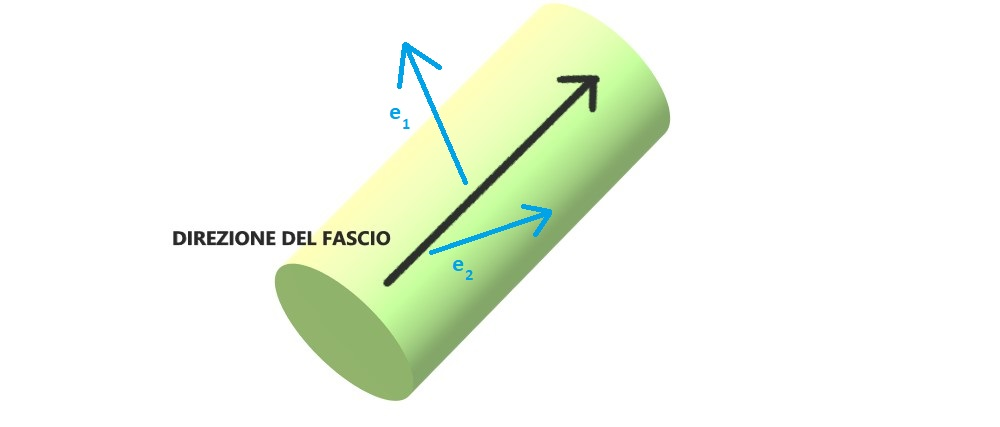
\includegraphics[width=0.72\linewidth]{let.jpg}
		\caption{Il cilindro schematizza la traiettoria di una particella del fascio. Gli elettroni $e_1$ ed $e_2$ possiedono energie rispettivamente $E_1>\Delta$ ed $E_2<\Delta$. Nella definizione di LET si considerano solo gli elettroni a corto raggio come $e_2$.}
		\label{fig:let}
	\end{figure}
	In base al valore di LET, è possibile distinguere due tipi di radiazione, quelle ad alto e basso LET. Le radiazioni a basso LET, disperdendo poca energia nei tessuti per unità di percorso, penetrano più in profondità rispetto alle radiazioni ad alto LET in quanto impiegano più tempo a esaurire l'energia che possiedono. Invece, le radiazioni ad alto LET arrecano danni biologici maggiori ai tessuti in quanto generano eventi di ionizzazione più frequenti e ravvicinati. La \hyperref[fig:damage_let]{Fig. 1.14} mostra che le radiazioni a basso LET, per esempio raggi X o $\gamma$, inducono prevalentemente danni isolati al DNA come le SSB mentre radiazioni ad alto LET, tra cui si trovano le particelle $\alpha$ o gli ioni pesanti, generano danni più distruttivi al DNA come le DSB \cite{Roobol2020-fp}.
	\begin{figure}[H]
		\centering
		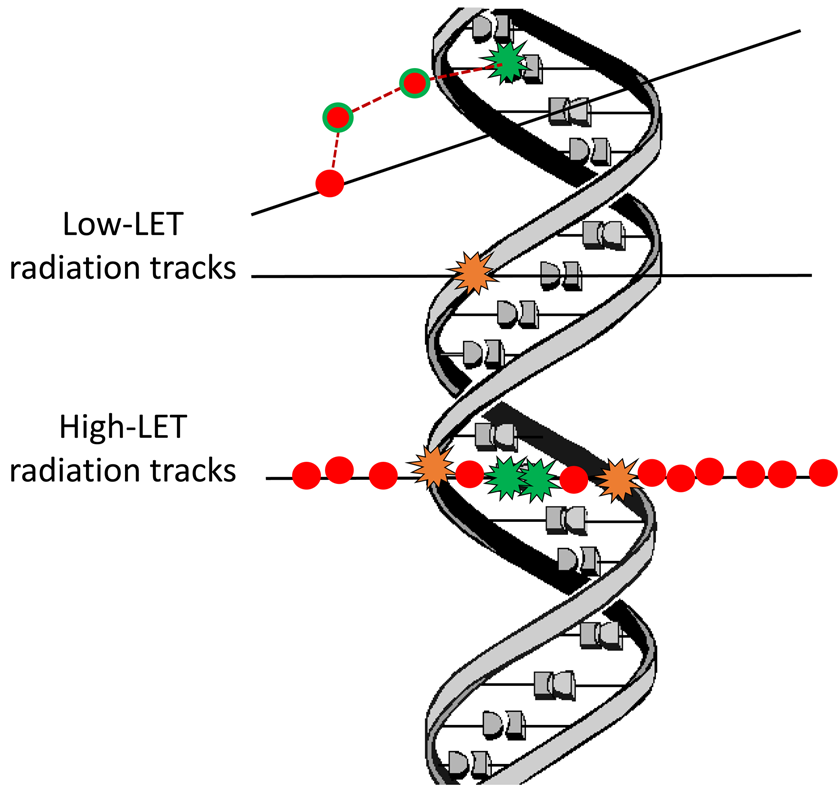
\includegraphics[width=0.6\linewidth]{damage_let.png}
		\caption{Danni tipici del DNA da parte di radiazioni a basso LET (in alto) e ad alto LET (in basso) \cite{Fabbrizi_Parsons_2022}.}
		\label{fig:damage_let}
	\end{figure}
	Dalla \hyperref[fig:proton_carbon_let]{Fig. 1.15} si osserva che i fasci adroterapici di protoni e ioni carbonio, decelerando, rilasciano una dose di energia crescente con la profondità nel materiale in cui penetrano, fin quando non si verifica un picco di perdita di energia in corrispondenza del picco di Bragg (Bragg Peak, BP), dopo il quale le particelle si fermano. La decelerazione di tali particelle, che avviene in maniera approssimativamente continua fino al BP, causa variazioni nella sezione d'urto delle particelle (si veda \hyperref[sec:sezione_urto]{Sez. 1.5.1}) che incrementano gli eventi di ionizzazione all'interno del materiale; per tale motivo, si osserva un aumento di LET durante il percorso delle particelle, che raggiunge un massimo in corrispondenza del BP. Inoltre, considerando i range energetici terapeutici, gli ioni carbonio possiedono valori di LET più alti rispetto a quelli dei protoni (si veda la \hyperref[tab:let_rbe]{Tab. 1.2}) poiché i primi possiedono una carica elettronica maggiore dei secondi che gli consente di effettuare molte più interazioni a parità di distanza percorsa e, di conseguenza, di generare danni più ingenti come le DSB, specialmente nella regione del BP (\hyperref[tab:let_rbe]{Tab. 1.2}).
	\begin{figure}[H]
		\centering
		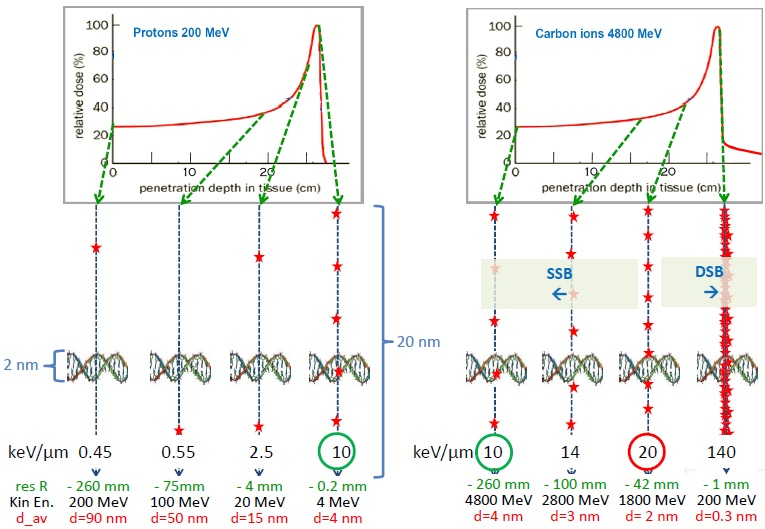
\includegraphics[width=0.9\linewidth]{proton_carbon_let.jpg}
		\caption{Distribuzione microscopica delle ionizzazioni adroniche in scala nanometrica con relativo LET, profondità raggiunta, energia cinetica e distanza media della creazione del danno \cite{slide_spighi}.}
		\label{fig:proton_carbon_let}
	\end{figure}
	In \hyperref[fig:proton_carbon_let]{Fig. 1.15} si nota che nel canale di ingresso, che corrisponde alla prima parte della penetrazione dove il rilascio di dose è minore, i protoni e gli ioni carbonio effettuano un danno rispettivamente ogni $90 \mbox{ nm}$ (insufficiente a colpire la doppia catena del DNA, il cui diametro è di $2 \mbox{ nm}$) e ogni $4 \mbox{ nm}$ (sufficiente a generare SSB), mentre in corrispondenza del BP i protoni e gli ioni carbonio effettuano un danno rispettivamente ogni $4 \mbox{ nm}$ e ogni $0.3 \mbox{ nm}$ (sufficienti a generare rispettivamente SSB e DSB). Pertanto, gli ioni carbonio sono più dannosi dei protoni in prossimità del BP, ma nel canale di ingresso causano molti più danni dei protoni; tale discordanza va tenuta conto in fase di TP affinché si selezioni il fascio adroterapico più adeguato alle specificità tumorali e tessutali del paziente.
	
	\subsubsection{Relative Biological Effectiveness}\label{par:rbe}
	La Relative Biological Effectiveness (RBE) di una radiazione ionizzante $R$ è un numero puro dato dal rapporto tra la dose $D_\gamma$ rilasciata dai raggi $\gamma$ e la dose $D_R$ rilasciata dalla radiazione $R$ al fine di ottenere lo stesso effetto biologico, fissato il \hyperref[sec:sopravvivenza_cellulare]{tasso di sopravvivenza delle cellule} $S$:
	\begin{equation}
		RBE=\frac{D^S_\gamma}{D^S_R}
		\label{eq:rbe}
	\end{equation}
	Ad esempio, se una radiazione $R$ ha $RBE>1$ significa che è necessaria una dose minore di $R$ per ottenere gli stessi danni biologici dei raggi $\gamma$ (in altre parole la radiazione $R$ è più efficace dei raggi $\gamma$). La valutazione dell'RBE è piuttosto complessa in quanto dipende dal tipo di radiazione, dall'energia della radiazione, dall'LET (\hyperref[fig:let_rbe]{Fig. 1.16a}), dal tipo di cellula e dal rateo di sopravvivenza della cellula (\hyperref[fig:survival_dose]{Fig. 1.16b}); in \hyperref[tab:let_rbe]{Tab. 1.2} si riportano dei valori di RBE per alcuni tipi di radiazione.
	\begin{figure}[H]
		\centering
		\begin{subfigure}[t]{0.49\textwidth}
			\centering
 			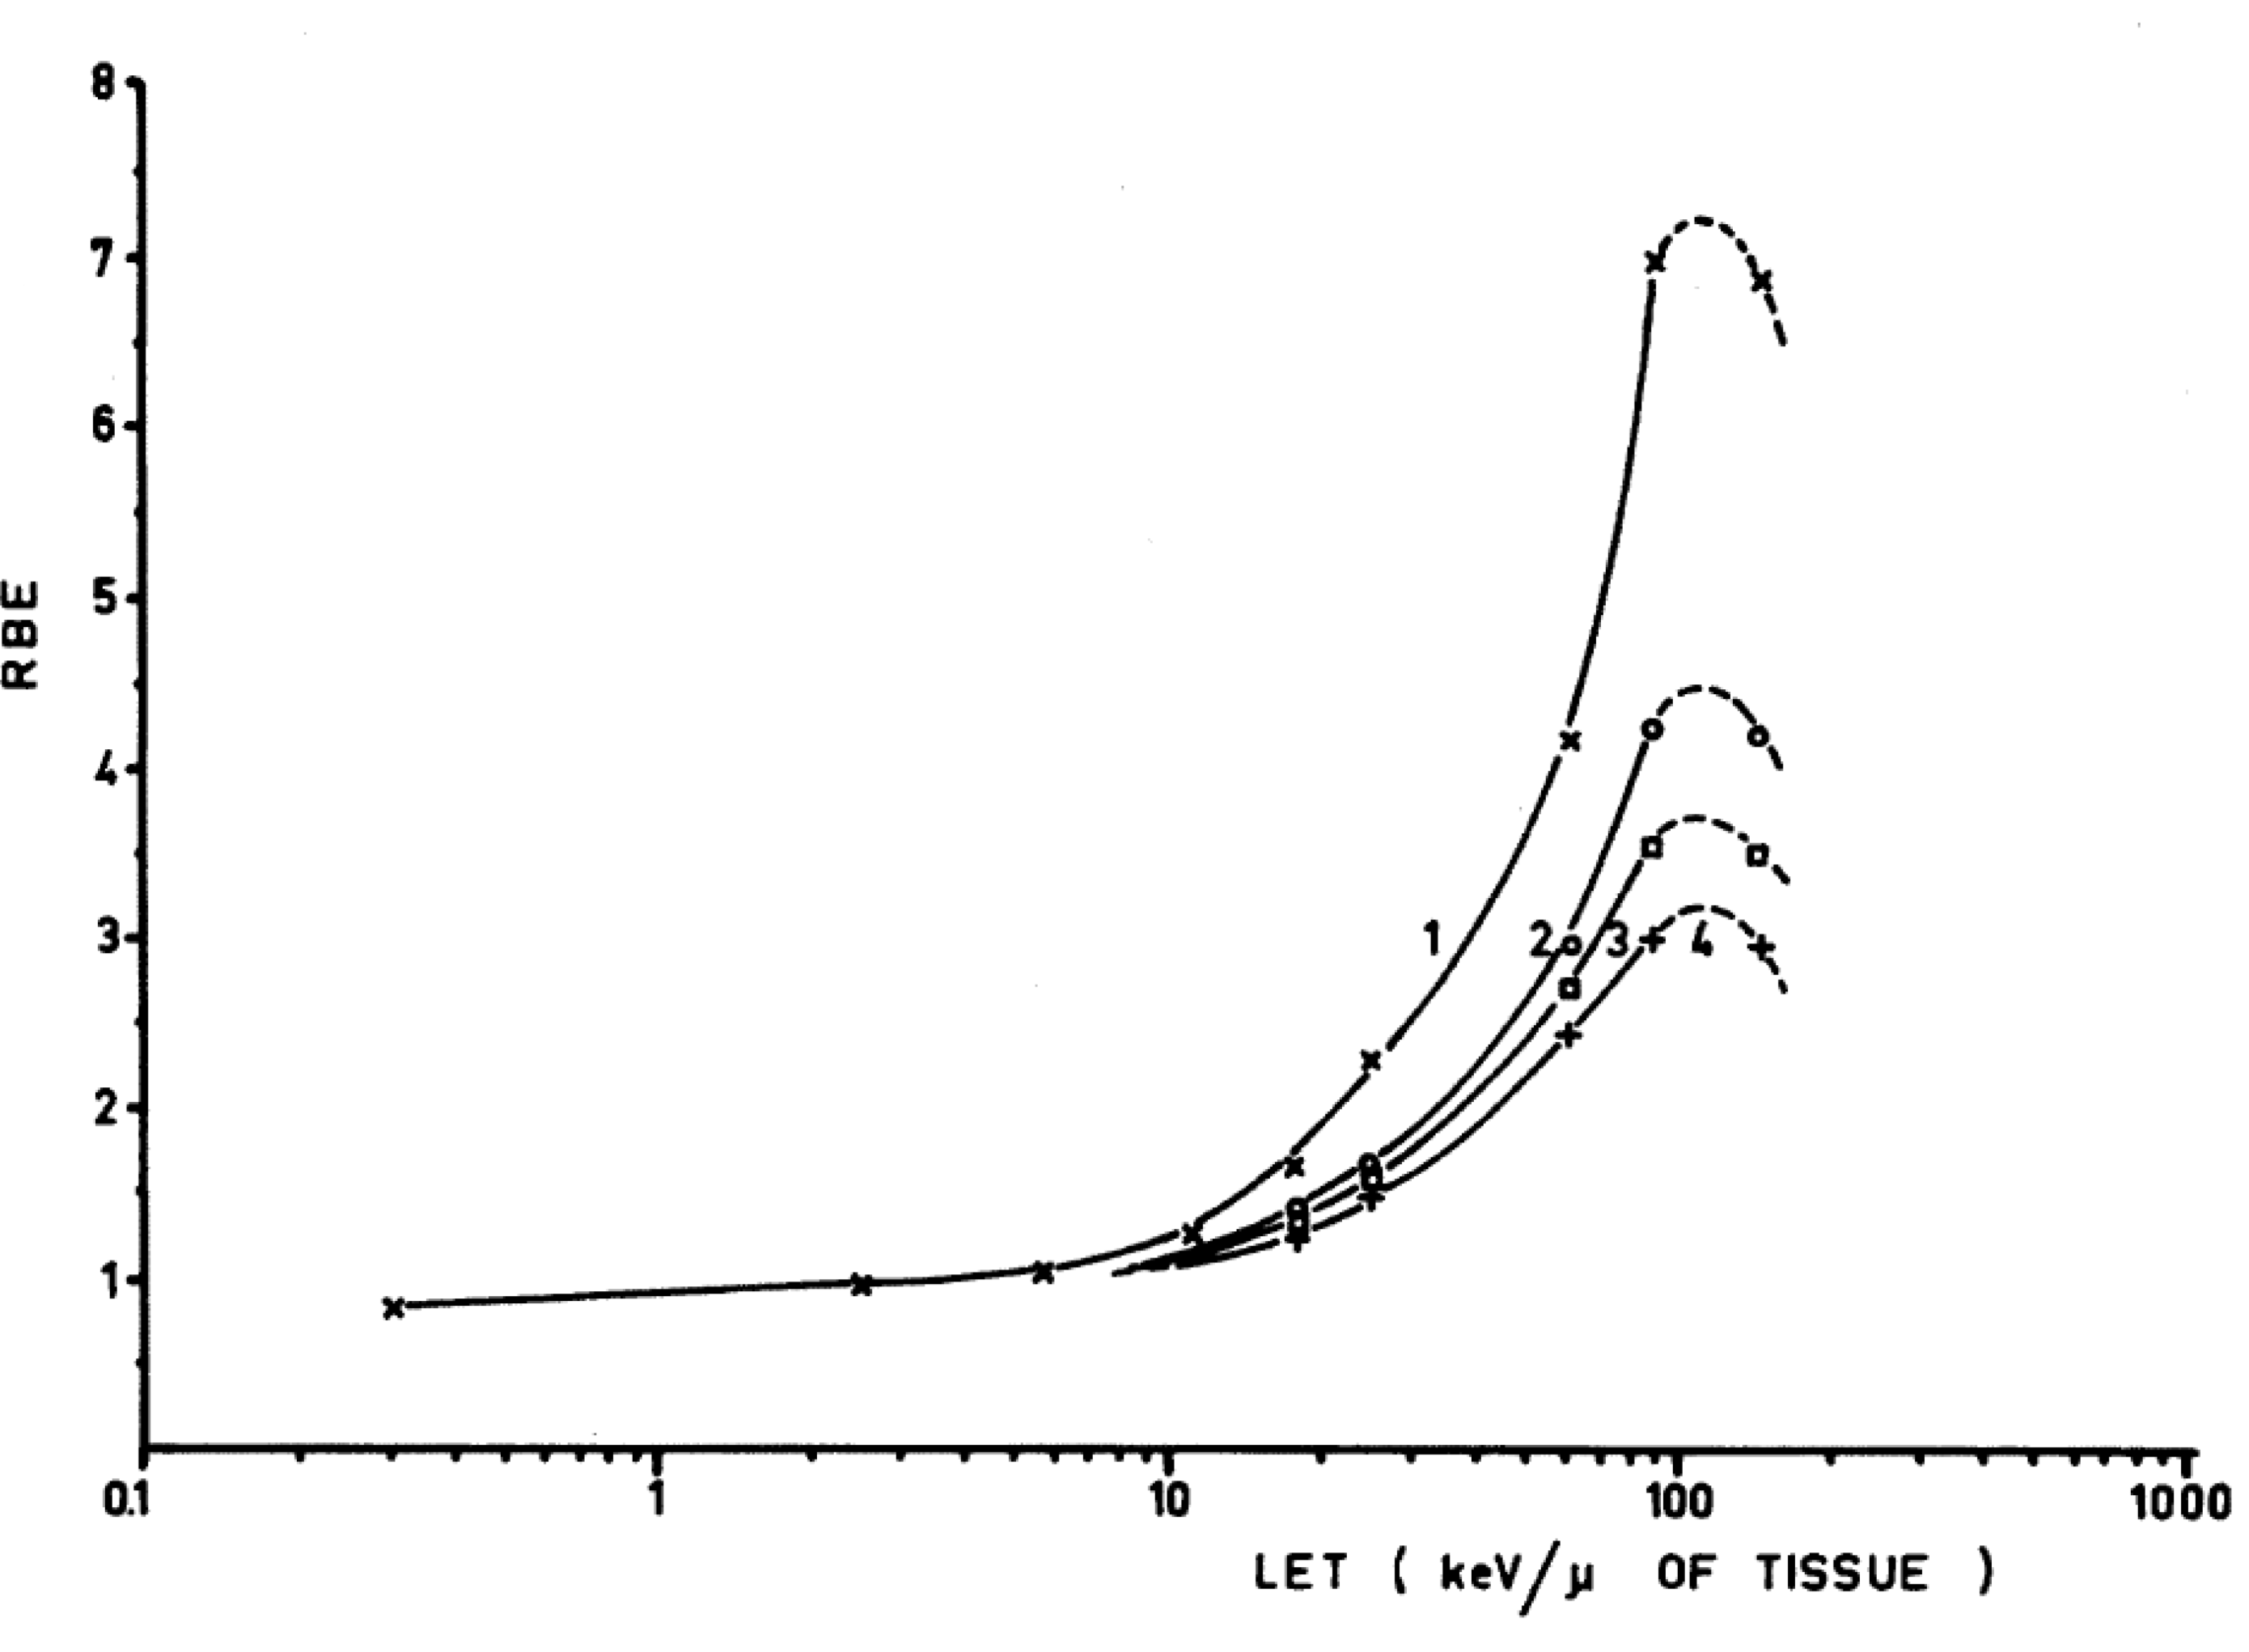
\includegraphics[width=\textwidth, scale=0.5]{let_rbe1.png}
			\caption{RBE in funzione dell'LET per cellule T1 renali umane irradiate con particelle pesanti cariche mono-energetiche. Le curve $1$, $2$ e $3$ corrispondono all'RBE misurato con frazioni di sopravvivenza cellulare rispettivamente di $0.8$, $0.1$ e $0.01$ \cite{antib1020124}.}
			\label{fig:let_rbe}
		\end{subfigure}
		\hfill
		\begin{subfigure}[t]{0.49\textwidth}
			\centering
			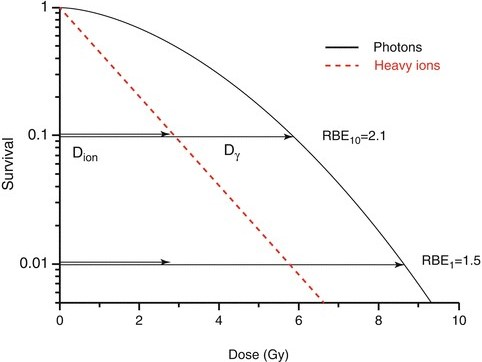
\includegraphics[width=\textwidth, scale=0.5]{survival_dose.jpg}
			\caption{Curve di sopravvivenza cellulare per fotoni e ioni in funzione della dose rilasciata e determinazione dell'RBE fissati i livelli di sopravvivenza del $10\%$ e dell'$1\%$ \cite{rad_key}.}
			\label{fig:survival_dose}
		\end{subfigure}
		\caption{Andamento dell'RBE in funzione dell'LET e del tasso di sopravvivenza della cellula.}
	\end{figure}
	\begin{table}[H]
		\centering
		\begin{tabular}{ |m{9.4cm}||M{3cm}|M{1cm}| }
			\hline
			Tipo di radiazione & LET $\left[\mbox{keV/}\mu\mbox{m}\right]$ & RBE\\
			\hline\hline
			Raggi X ($6$--$15 \mbox{ MeV}$) & $0.3$ &	$\approx 0.8$\\
			\hline
			Particella $\beta$ ($1 \mbox{ MeV}$) & $0.3$ & $0.9$\\
			\hline
			Raggi $\gamma$ ($1 \mbox{ MeV}$) & $0.5$ & $1$\\
			\hline
			Protoni a energie terapiche ($150 \mbox{ MeV}$) & $0.5$ & $\approx1.1$\\
			\hline
			Neutroni & $0.5$--$100$ & $1$--$2$\\
			\hline
			Particella $\alpha$ & $50$--$200$ & $5$--$10$\\
			\hline
			Ioni carbonio nella regione vicina al picco di Bragg & $40$--$90$ & $2$--$5$\\
			\hline
		\end{tabular}
		\caption{Valori approssimati di LET e RBE di alcuni tipi di radiazione \cite{MURSHED201957}.}
		\label{tab:let_rbe}
	\end{table}
	\begin{figure}[H]
		\centering
		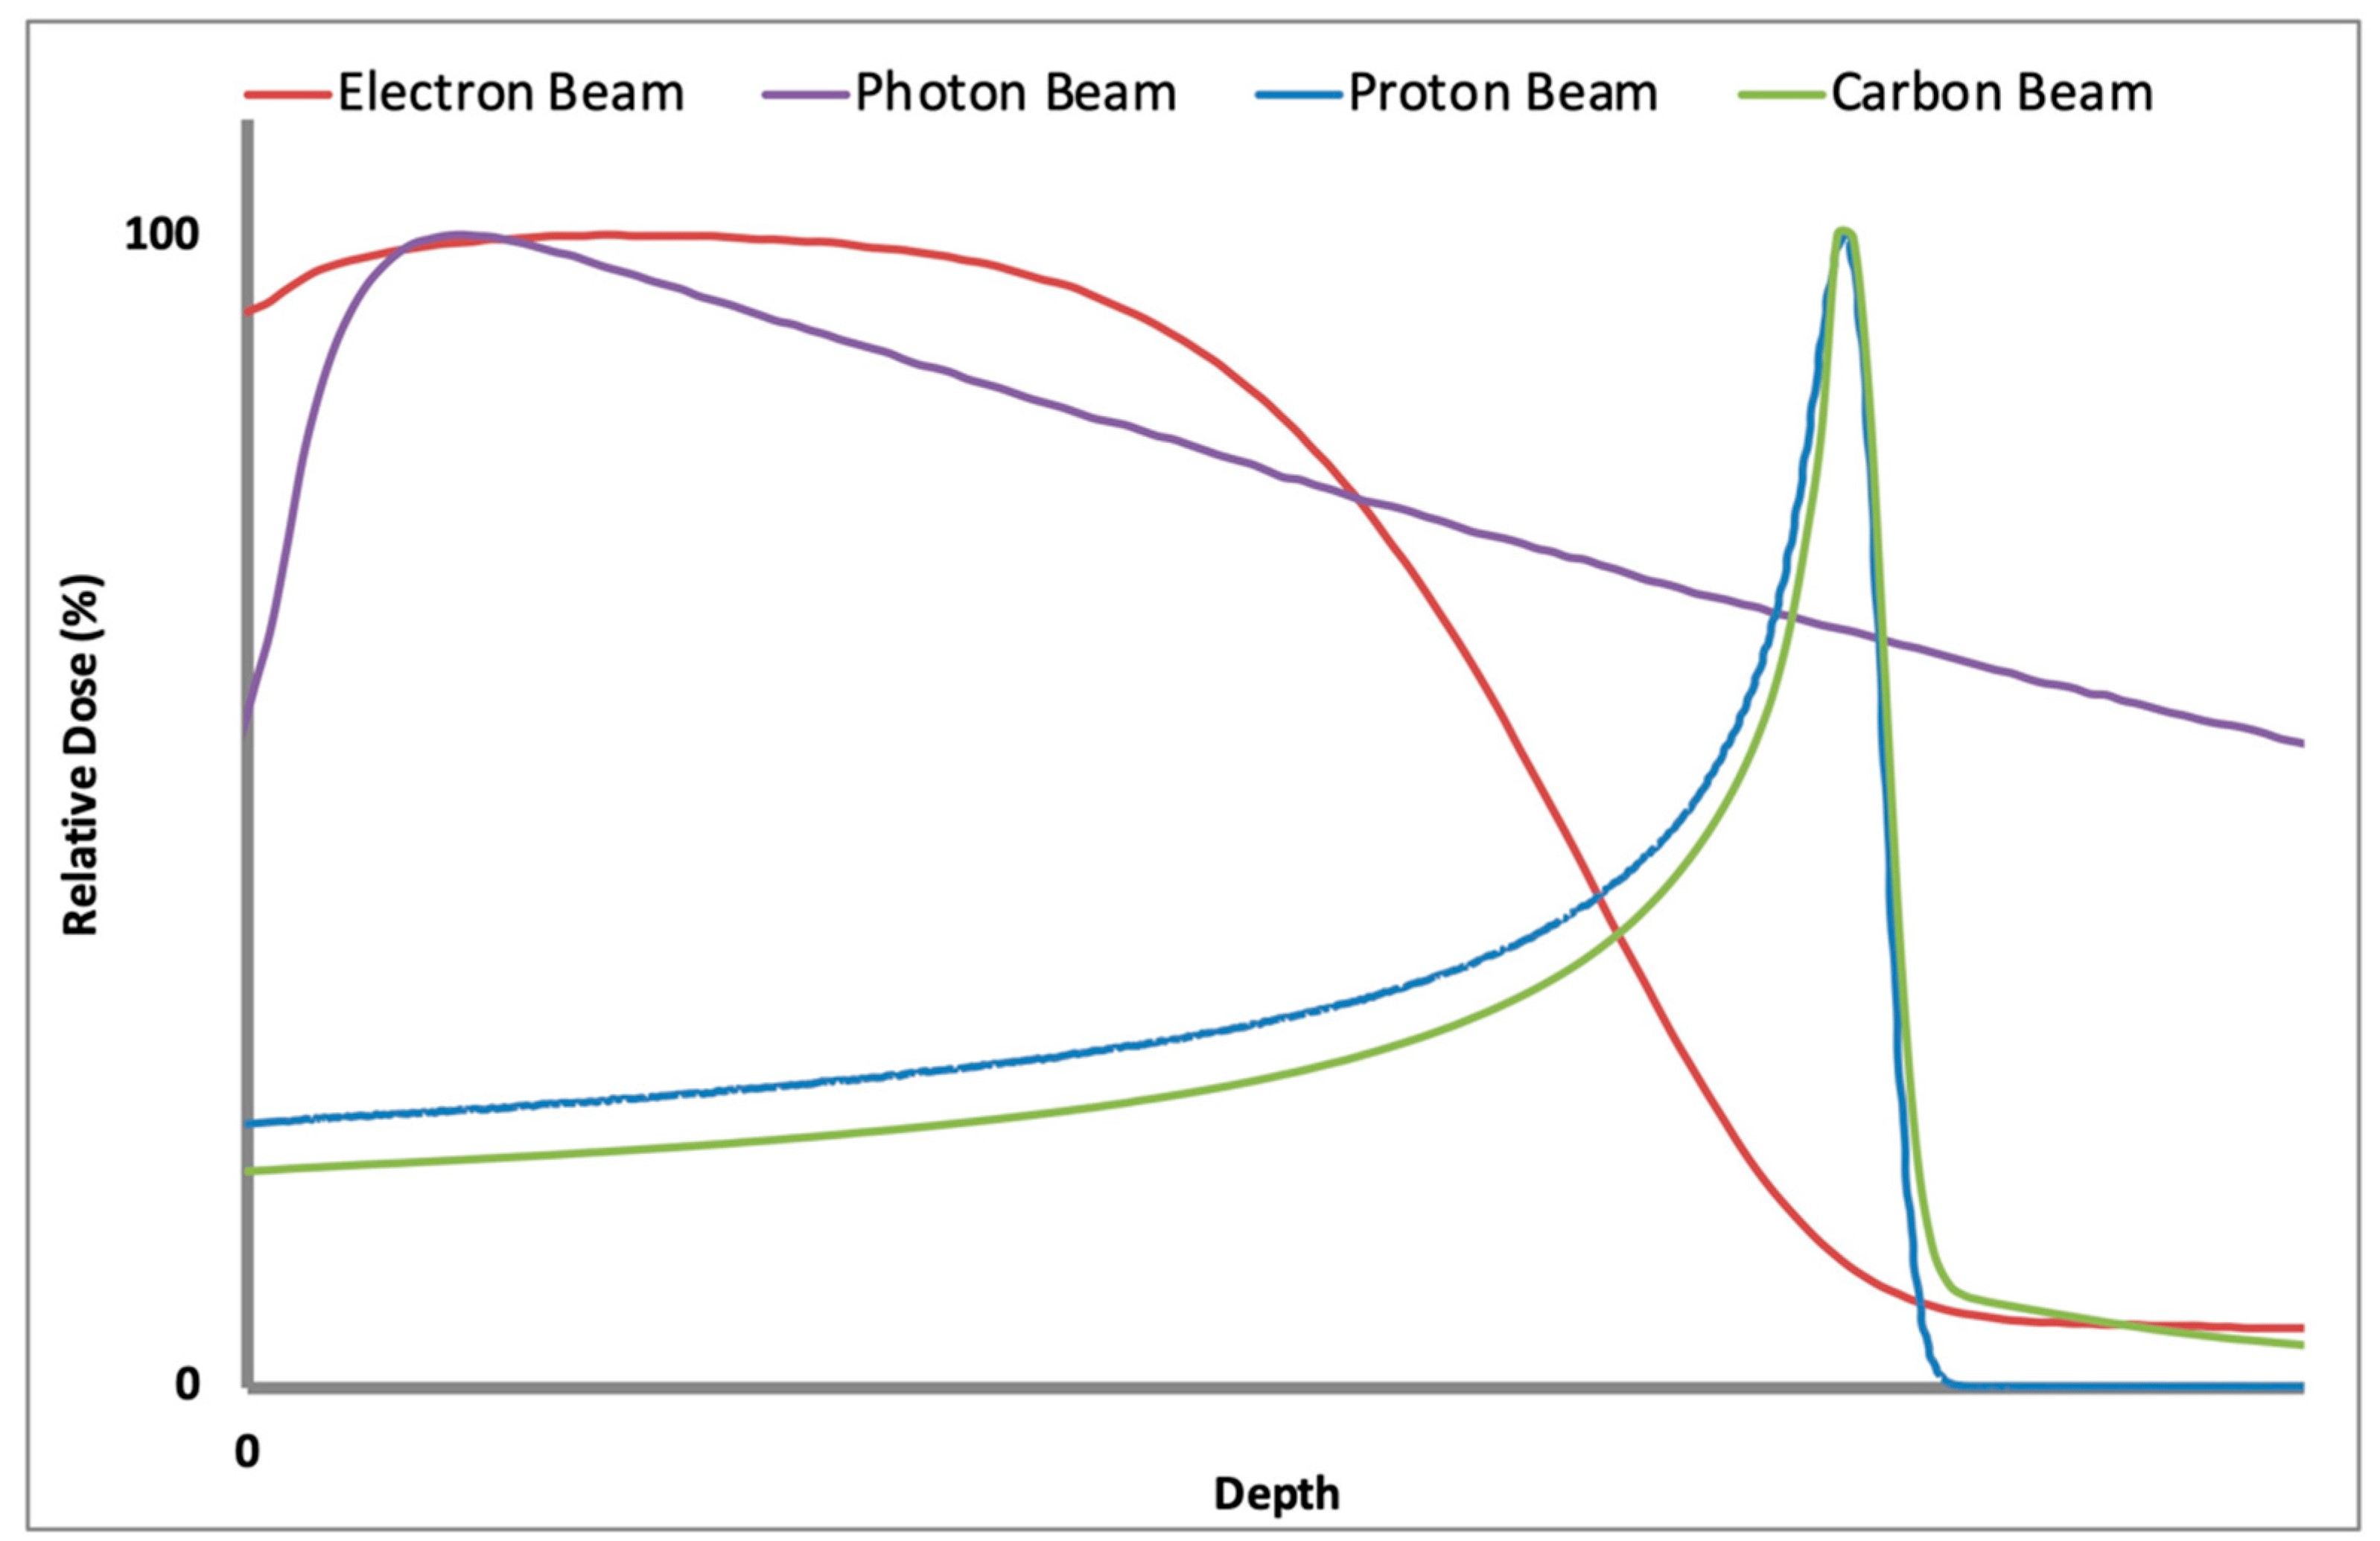
\includegraphics[width=0.9\linewidth]{photon.jpg}
		\caption{Rilascio di dose relativa in funzione della profondità del tessuto per fotoni, elettroni, ioni carbonio e protoni (normalizzati allo stesso massimo). Si notino i picchi di Bragg sia per gli ioni carbonio che per i protoni (particelle usate in adroterapia), assenti per elettroni e fotoni (particelle usate in radioterapia) \cite{biomedicines9010031}.}
		\label{fig:photon}
	\end{figure}
	Dalla \hyperref[tab:let_rbe]{Tab. 1.2} si nota che i fasci adroterapici di ioni carbonio sono molto più efficienti dei fasci radioterapici fotonici (raggi $\gamma$). I protoni, invece, possiedono un RBE solo del $10\%$ più grande rispetto ai fotoni; tale somiglianza non sembrerebbe coadiuvare le riflessioni esposte nella \hyperref[sec:1.2]{Sez. 1.2}, in cui si sono evidenziati i grandi vantaggi della protonterapia sulla radioterapia in relazione al rilascio di dose più potente della prima sulla seconda. In realtà l'efficienza protonterapica vince su quella radioterapica se si tengono conto degli effetti globali di entrambe le radiazioni: mentre i protoni (così come gli ioni carbonio) rilasciano la maggior parte della dose in una zona ristretta situata in prossimità del BP, i fotoni rilasciano la dose in una regione molto più ampia (aumentando il rischio di colpire organi sani), come evidenziato nella \hyperref[fig:photon]{Fig. 1.17}.
	
	Per i motivi sopra citati, negli ultimi anni la variabilità dell'RBE protonico è stata ampiamente dibattuta; alcuni studi riportano misure radiobiologiche che attestano valori superiori rispetto all'$1.1$ riportato in \hyperref[tab:let_rbe]{Tab. 1.2} \cite{Tang1997-wb}. In particolare, nella ref. \cite{cancers7010353} si propone che l'aumento dell' RBE protonico sia causato dalle particelle prodotte nella frammentazione nucleare del target\footnote{In fisica nucleare e subnucleare il target (o targhetta) è una porzione di materia che funge da bersaglio di un fascio di particelle inviato per studiare la materia, il fascio e le loro interazioni \cite{treccani_target}.} (quest'ultimo corrispondente ai nuclei del corpo umano): nell'attraversare il paziente, le \hyperref[par:interazioni_nucleari]{interazioni nucleari} che intercorrono tra il fascio protonico e i tessuti del paziente stesso generano dei frammenti, particelle secondarie caratterizzate da un corto raggio ($10$--$100\mu\mbox{ m}$), alto LET e alto RBE. Uno degli obiettivi primari dell'esperimento FOOT è proprio quello di migliorare l'accuratezza dell'RBE protonico (in funzione di profondità e tipo di tessuto) a partire dalla misura di sezioni d'urto differenziali, energie e direzioni dei frammenti; conoscere minuziosamente tali grandezze porterebbe a valutazioni più precise degli effetti biologici protonterapici e a una conseguente riduzione dei margini di errore in fase di TP.
		
	Nel corso del tempo molti studi si sono incentrati sul legame tra RBE e LET, fortemente dipendente dalla natura del materiale biologico e dalla scelta dell'endpoint utilizzato per definire l'efficacia radioterapica. Pur fissando tali parametri, alcuni risultati mostrano che radiazioni differenti aventi stessi LET possiedono diversi RBE \cite{jicru}. Nonostante tali difficoltà, la \hyperref[fig:let_rbe]{Fig. 1.16a} riporta un tipico andamento di RBE e LET in cui si osserva che l'RBE aumenta al crescere dell'LET fino a raggiungere un massimo intorno ai $100\mbox{keV}/\mu\mbox{m}$, dopo il quale si verifica una forte diminuzione. La spiegazione del primo tratto è ovvia, in quanto più energia assorbe il materiale attraversato da radiazione più danni biologici saranno arrecati allo stesso, mentre nel secondo tratto si verifica un fenomeno di saturazione denominato overkill cellulare in cui la quantità di energia che viene depositata è così elevata che si produce una quantità di danni al DNA maggiore di quella richiesta per la morte cellulare, da cui consegue la riduzione dell'efficacia biologica del trattamento \cite{linz2011ion}.
	\begin{figure}[H]
		\centering
		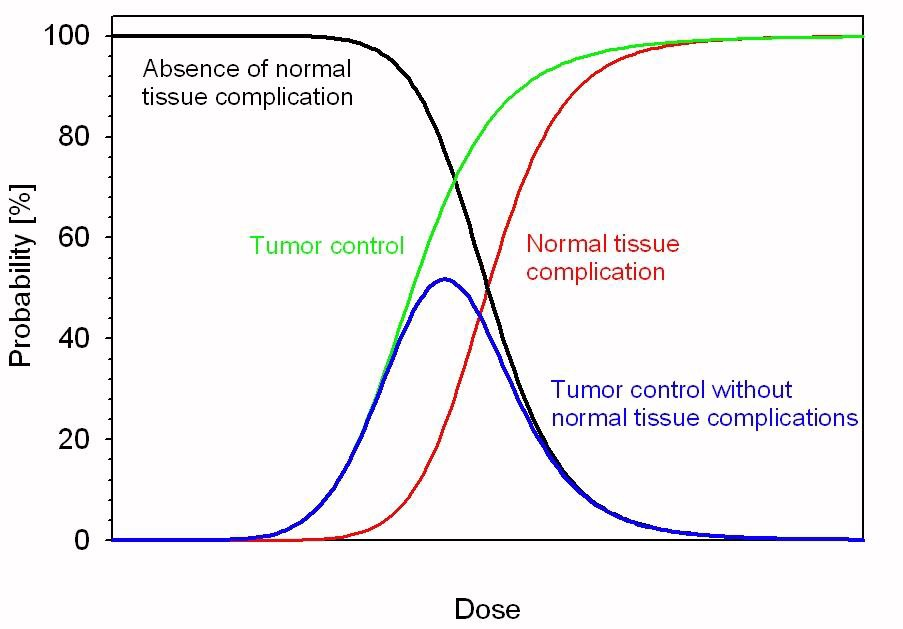
\includegraphics[width=0.9\linewidth]{tcp.jpg}
		\caption{Andamenti del TCP (in verde), dell'NTCP (in rosso), della loro differenza (in blu) e dell'assenza di complicazioni nei tessuti sani (in nero) in funzione della dose rilasciata nei tessuti. Il range di dose ottimale nei trattamenti si trova in corrispondenza della curva blu \cite{Jensen2019}.}
		\label{fig:tcp}
	\end{figure}
	Comprendere quale sia il range di dose più efficace nei trattamenti radio e adroterapici è molto complesso in quanto gli effetti radiobiologici dipendono da molti parametri, alcuni dei quali vengono analizzati nei paragrafi successivi. In generale, durante il TP dei pazienti affetti da tumore, sono due i fattori che influenzano la scelta della dose: il TCP (Tumor Control Probability) e l'NTCP (Normal Tissue Complication Probability). Lo scopo di radio e adroterapia è quello di raggiungere un'elevata probabilità di controllare localmente un tumore (che corrisponde a un alto valore di TCP) mantenendo bassa la probabilità di sviluppare complicazioni nei tessuti sani (che corrisponde all'NTCP) \cite{Baumann2005-kp}. Teoricamente, il range di dose più efficiente è quello che massimizza il TCP e minimizza l'NTPC (in altre parole il range di dose ottimale è quello che massimizza la differenza tra TCP e NTCP). Dato che le cellule sane sono in grado di riparare i danni radiativi meglio delle cellule cancerose, tale range esiste (pur essendo fortemente dipendente dal tipo di tumore e dal suo stadio) e si attesta intorno a $20$--$80\mbox{ Gy}$, valori letali se rilasciati in un'unica seduta (questo è uno dei motivi per cui si effettua il frazionamento, si veda \hyperref[sec:sopravvivenza_cellulare]{Sez. 1.4.3}). Tali considerazioni sono riassunte in \hyperref[fig:tcp]{Fig. 1.18}.

	\subsubsection{Oxygen Enhancement Ratio}\label{par:oer}
	L'Oxygen Enhancement Ratio (OER) è un numero puro che misura l'efficacia biologica della radiazione in relazione alla concentrazione di ossigeno presente nei tessuti. Infatti, come già riportato nell'analisi del \hyperref[par:danno_indiretto]{danno indiretto} della radiolisi dell'acqua, se il tessuto colpito con radiazione ionizzante presenta un'abbondanza di ossigeno (iperossia) si genera un numero maggiore di radicali liberi e, di conseguenza, aumentano le probabilità di danno al DNA del tessuto irradiato, come mostrato in \hyperref[fig:oer_survival]{Fig. 1.19}. L'OER è definito come il rapporto tra la dose di una certa radiazione in condizioni di mancanza di ossigeno (anossia) $D_{anossia}$ e la dose della stessa radiazione in normali concentrazioni di ossigeno $D_{normale}$:
	\begin{equation}
		OER=\frac{D_{anossia}}{D_{normale}}
		\label{eq:oer}
	\end{equation}
	\begin{figure}[H]
		\centering
		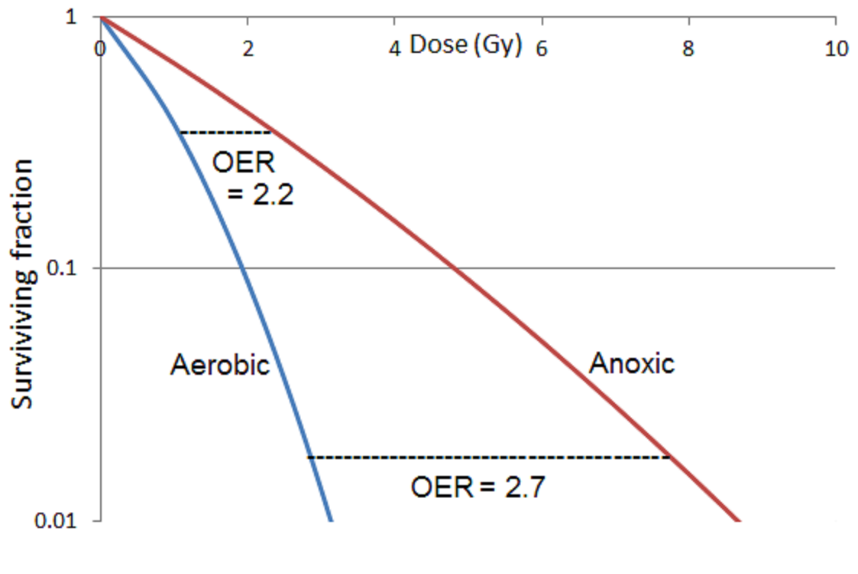
\includegraphics[width=0.73\linewidth]{oer_survival.png}
		\caption{A parità di percentuale di cellule sopravvissute, per arrecare danni biologici in normali condizioni aerobiche (presenza di ossigeno) è necessaria una dose inferiore rispetto alle condizioni di anossia; maggiore è la concentrazione di ossigeno, maggiore è la probabilità di effettuare dei danni \cite{ox_effect_wiki}.}
		\label{fig:oer_survival}
	\end{figure}
	L'OER decresce all'aumentare dell'LET della radiazione ionizzante, come evidenziato in \hyperref[fig:let_oer]{Fig. 1.20a}. Nelle radiazioni a basso LET si verificano eventi di ionizzazione isolati che favoriscono la \hyperref[eq:prodotto1]{Eq. 1.4a}, da cui si ottiene un'innocua molecola d'acqua (\ce{H2O}); per questo motivo, l'aggiunta di atomi di ossigeno aumenta notevolmente i danni biologici arrecati ai tessuti e il valore dell'OER si attesta attorno a $2$--$4$. Al contrario, nelle radiazioni ad alto LET si verificano eventi di ionizzazione frequenti che favoriscono la \hyperref[eq:prodotto2]{Eq. 1.4b}, da cui si ottiene una dannosa molecola di perossido di idrogeno (\ce{H2O2}); per tale ragione, l'aggiunta di atomi di ossigeno risulta superflua per l'amplificazione dei danni biologici, dato che l'ambiente è già ricco di \ce{H2O2}, e il valore dell'OER si attesta attorno all'unità \cite{BRAHME2014121,Barendsen1994-bx}. In \hyperref[fig:reaction_let]{Fig. 1.20b} si riassumono le reazioni chimiche favorite in regime di alto e basso LET.
	\begin{figure}[H]
		\centering
		\begin{subfigure}[t]{0.49\textwidth}
			\centering
			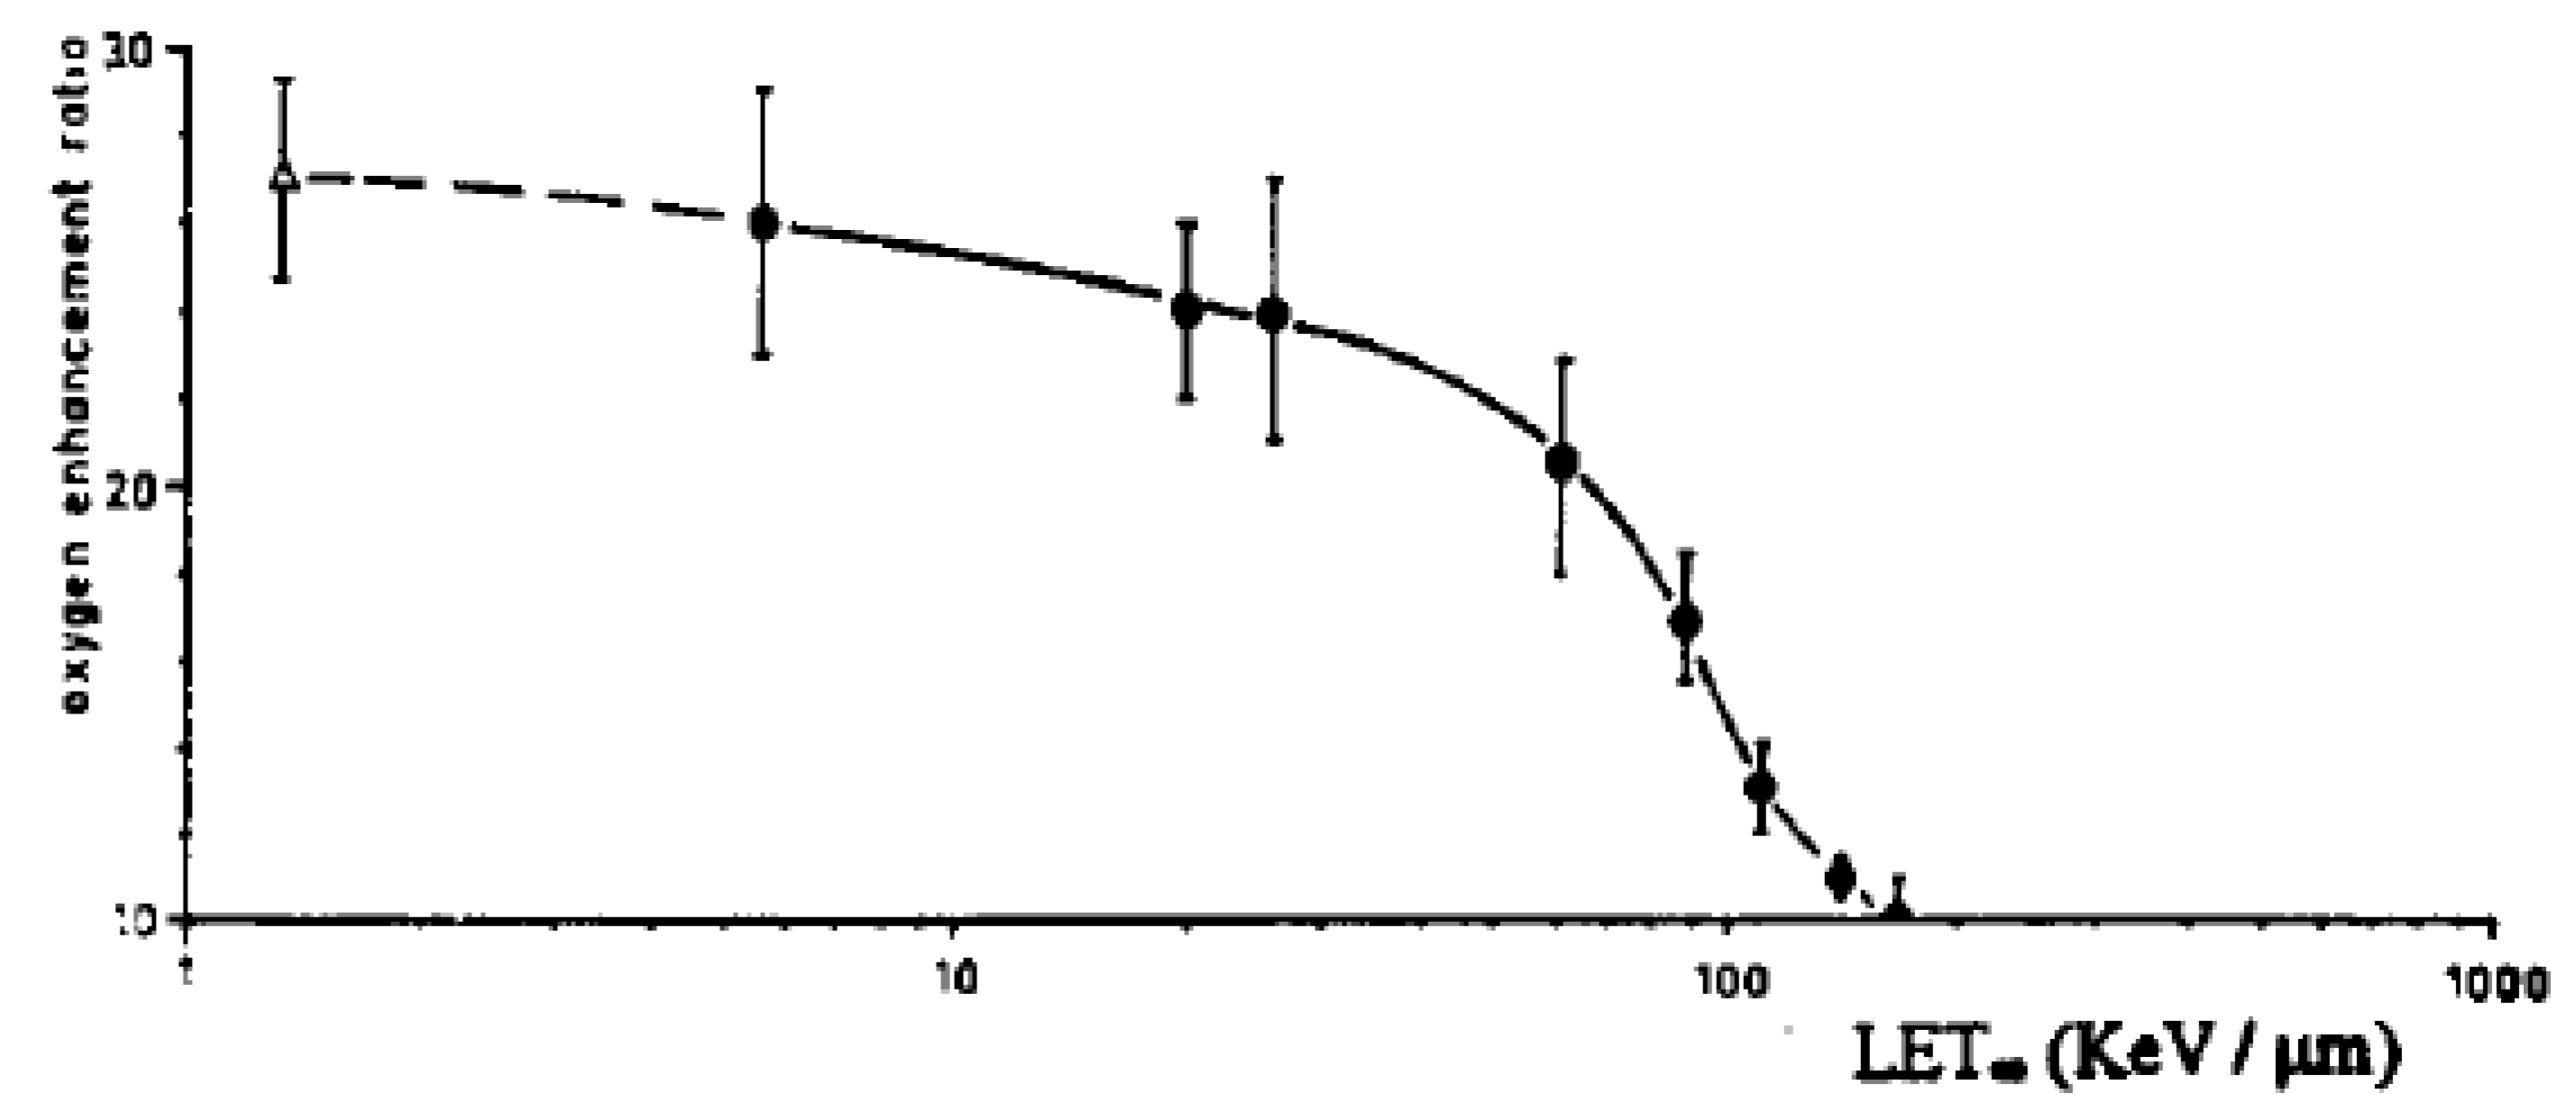
\includegraphics[width=\textwidth, scale=0.50]{let_rbe2.png}
			\caption{Andamento dell'OER in funzione dell'LET per particelle $\alpha$ mono-energetiche \cite{antib1020124,handbook1}.}
			\label{fig:let_oer}
		\end{subfigure}
		\hfill
		\begin{subfigure}[t]{0.49\textwidth}
			\centering
			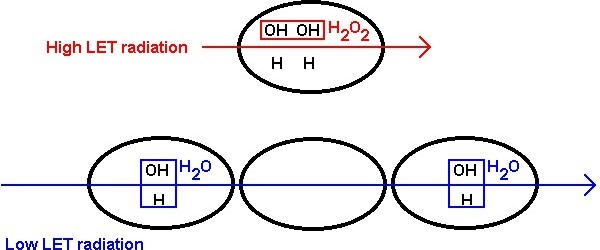
\includegraphics[width=\textwidth, scale=0.50]{reaction_let.jpg}
			\caption{Schematizzazione delle reazioni più comuni per radiazioni ad alto LET (in alto) e a basso LET (in basso) \cite{let_si}.}
			\label{fig:reaction_let}
		\end{subfigure}
		\caption{Rapporto tra l'OER e le radiazioni ad alto e basso LET.}
	\end{figure}
	Spesso accade che la proliferazione di un tumore diventa talmente rapida che il suo apporto di sangue non è sufficiente a ossigenare alcune sue parti, generando microambienti ipossici che rendono il tumore stesso non solo più incline ad andare incontro a metastasi \cite{Carmeliet2011-ua}, ma anche più radioresistente \cite{Gilkes2014-rw}. Per risolvere tale problematica si sono effettuati numerosi approcci sistemici, dal posizionare i pazienti in camere iperbariche\footnote{La camera iperbarica è un luogo in cui il paziente respira un'aria ricca di ossigeno.} prima di procedere con le sedute radioterapiche all'uso di farmaci in grado di incrementare il flusso sanguigno o l'emoglobina\footnote{L'emoglobina è una proteina deputata per il trasporto di ossigeno nel sangue.}, risultati insoddisfacenti in quanto i meccanismi omeostatici del corpo umano riescono ugualmente a stabilizzare i livelli di ossigeno. Solo recentemente si sono sviluppati nuovi metodi più efficaci in grado di aumentare localmente la concentrazione di ossigeno, come l'iniezione di ``microbolle'' nel flusso sanguigno umano \cite{ox_microbubbles}. In generale, tutte le metodiche di incremento dell'ossigeno sopra citate risulterebbero potenzialmente utili ad amplificare i danni indiretti al DNA, ma dall'altra renderebbero più ossigenate anche aree popolate da organi sani, che verrebbero rese più sensibili ai danni provocati dalla radiazione \cite{ox_radiation_t}.
	
	\subsection{Sopravvivenza cellulare}\label{sec:sopravvivenza_cellulare}
	\begin{figure}[H]
		\centering
		\begin{subfigure}[t]{0.49\textwidth}
			\centering
			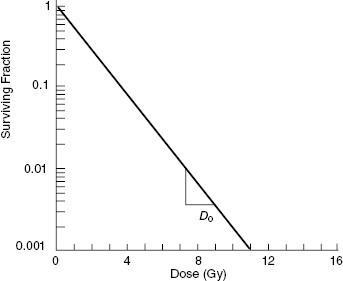
\includegraphics[width=\textwidth, scale=0.50]{survival1.jpg}
			\caption{Sopravvivenza cellulare di un batterio Escherichia coli. $D_0$ è la dose che riduce la sopravvivenza di un fattore $1/e$ \cite{rad_key2}.}
			\label{fig:survival1}
		\end{subfigure}
		\hfill
		\begin{subfigure}[t]{0.49\textwidth}
			\centering
			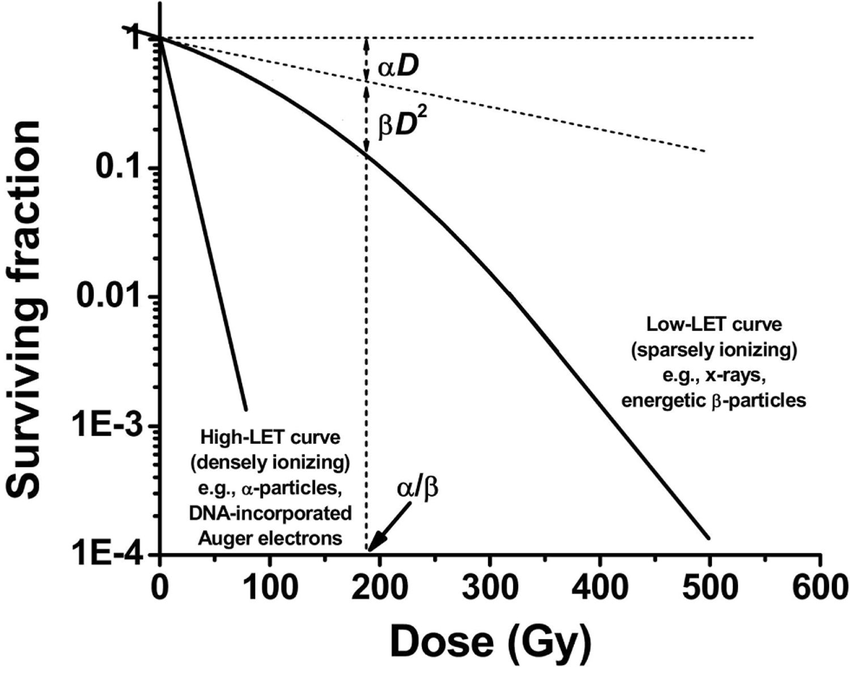
\includegraphics[width=\textwidth, scale=0.50]{survival2.png}
			\caption{Sopravvivenza cellulare di una cellula di mammifero dopo un irraggiamento ad alto e basso LET. Un rilascio a basso LET arreca un numero minore di danni, evidente da un appiattimento della pendenza della curva di sopravvivenza indotto dai meccanismi di riparazione del DNA \cite{radionuclides1}.}
			\label{fig:survival2}
		\end{subfigure}
		\caption{Decadimenti esponenziali della sopravvivenza cellulare in funzione della dose in scala semilogaritmica.}
	\end{figure}
	Dopo aver discusso delle principali grandezze fisico-mediche con cui si valutano gli effetti biologici della radiazione ionizzante, è necessario analizzare i modelli che descrivono la sopravvivenza cellulare. Innanzitutto, gli eventi di ionizzazione prodotti dalla radiazione sono processi stocastici. Pertanto, la morte cellulare segue leggi probabilistiche dettate dalla statistica di Poisson. Per esempio, consideriamo una dose che, rilasciata una prima volta, riduce la sopravvivenza cellulare del $50\%$; un secondo rilascio ridurrebbe la sopravvivenza al $25\%$, un terzo al $12.5\%$ e così via. Seguendo tale ragionamento, in prima approssimazione è possibile considerare la legge mostrata in \hyperref[eq:survival1]{Eq. 1.15}, che descrive la frazione di cellule sopravvissute $S$ in funzione della dose rilasciata $D$:
	\begin{equation}
		S=e^{-0.69D}
		\label{eq:survival1}
	\end{equation}
	In realtà l'\hyperref[eq:survival1]{Eq. 1.15}, il cui andamento è rappresentato in \hyperref[fig:survival1]{Fig. 1.21a}, descrive il tasso di sopravvivenza per cellule procarioti (come quelle dei batteri), le quali non sono sostanzialmente in grado di riparare i danni radiativi attivando sistemi di riparazione. Al contrario, le cellule degli esseri umani (in generale le cellule eucarioti dei mammiferi) possiedono complessi meccanismi di riparazione del DNA (accennati nell'analisi dei \hyperref[par:danno_diretto]{danni diretti}) che consentono di recuperare i danni dovuti a radiazioni ionizzanti. Suddetti meccanismi, però, sono efficaci solo in presenza di un basso rilascio di dose (basso LET), mentre per alte energie depositate (alto LET) non sono sufficienti a riparare i danni radiativi; questi ultimi, infatti, per alte energie depositate risultano addirittura maggiori rispetto a quelli arrecati a cellule batteriche. Quindi, gli effetti dei meccanismi di riparazione incidono nell'andamento della sopravvivenza cellulare solo in un regime di basso LET, come illustrato in \hyperref[fig:survival2]{Fig. 1.21b}.
	
	In considerazione dell'analisi di cui sopra, l'ICRP (International Commission on Radiological Protection) approvò nel $1991$ un accurato modello radiobiologico in grado di descrivere accuratamente la sopravvivenza cellulare in seguito al rilascio di radiazione ionizzante \cite{icrpAnn}. Tale modello, chiamato LQ (Lineare Quadratico), prevede che la frazione di cellule sopravvissute $S$ in funzione della dose rilasciata $D$ sia descritta dalla \hyperref[eq:survival2]{Eq. 1.16}:
	\begin{equation}
		S=e^{-\alpha D-\beta D^2}
		\label{eq:survival2}
	\end{equation}
	dove $\alpha$ e $\beta$ sono due parametri dipendenti dal tessuto, dalla radiazione e dallo stato di salute cellulare tali che $\left[\alpha\right]\mbox{Gy}^{-1}$ e $\left[\beta\right]\mbox{Gy}^{-2}$. In particolare, il fattore lineare $\alpha D$ rappresenta gli eventi di ``hit singola'', in cui il danno cellulare viene provocato da una singola particella incidente, mentre il fattore quadratico $\beta D^2$ rappresenta gli eventi di ``hit multipla'', in cui il danno cellulare deriva dall'azione di una doppia traccia di particelle (si veda \hyperref[fig:survival_cell]{Fig. 1.22}). In sostanza, $\alpha$ misura la parte dei danni letali non riparabili e rappresenta principalmente gli eventi di DSB, mentre $\beta$ misura la parte dei danni sub-letali\footnote{Un danno sub-letale è un tipo di danno non letale di per sé, ma che può diventarlo se combinato a ulteriori danni indotti dalle radiazioni \cite{McMahon_2019}.} riparabili e rappresenta maggiormente gli eventi di SSB.
	\begin{figure}[H]
		\centering
		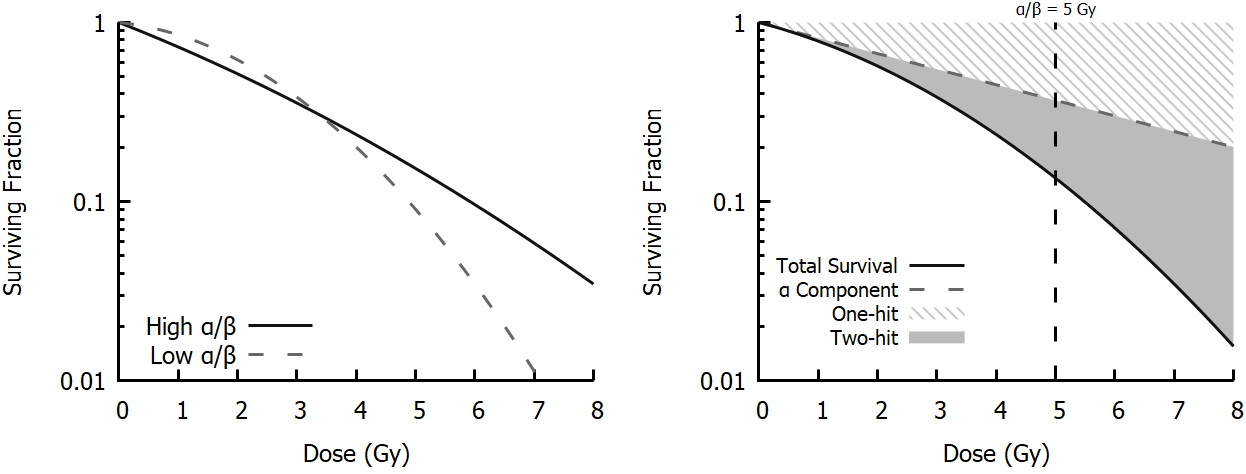
\includegraphics[width=0.9\linewidth]{survival_cell.jpg}
		\caption{Andamento della sopravvivenza cellulare in funzione della dose rilasciata. Sinistra: risposte cellulari differenti corrispondenti a diversi valori di $\alpha/\beta$. Le curve con alto $\alpha/\beta=10\mbox{ Gy}$ possiedono tassi quasi costanti di morte cellulare mentre le curve con basso $\alpha/\beta=3\mbox{ Gy}$ mostrano una curvatura pronunciata, con una morte cellulare che aumenta al crescere della dose rilasciata. Destra: separazione della curva di sopravvivenza cellulare in cinetica a singola e a doppia hit. Per basse dosi la cinetica prevalente è quella a singola hit ($S\approx e^{-\alpha}$), mentre a dosi più alte domina la cinetica a hit multipla. Gli effetti di cinetica a singola e a doppia hit sono equivalenti quando $D=\alpha/\beta=5\mbox{ Gy}$ \cite{McMahon_2019}.}
		\label{fig:survival_cell}
	\end{figure}
	I modelli di sopravvivenza cellulare per le cellule mammifere, uniti al fatto che le cellule sane recuperano danni più facilmente di quelle cancerose, suggeriscono che per eliminare una neoplasia è opportuno effettuare più dosi a bassa energia piuttosto che un'unica dose ad alta energia, in un processo chiamato frazionamento. Quest'ultimo viene impiegato per sfruttare al massimo la capacità riparatrice delle cellule sane, al fine di risparmiare tessuti e organi non malati che, inevitabilmente, vengono colpiti anche in minima parte nei trattamenti radio e adroterapici (in radioterapia ciò è più frequente che in adroterapia, come illustrato dai profili di dose in \hyperref[fig:photon]{Fig. 1.17}). L'intervallo temporale che intercorre tra un rilascio di dose e l'altro non deve essere né troppo breve (si deve evitare che le cellule danneggiate dei tessuti sani vengano uccise dando i giusti tempi di recupero\footnote{Solitamente le cellule sane riparano i danni biologici dopo almeno sei ore \cite{Chang2021}.}), né troppo lungo (altrimenti l'effetto combinato delle sedute radioterapiche risulterebbe vano rispetto a un unico rilascio di dose). Tipicamente, il trattamento radioterapico viene frazionato in $30$--$35$ sedute effettuate giornalmente, in modo che le $24$ ore di attesa tra una seduta e l'altra consentano alle cellule sane di riparare molti più danni rispetto a quelle tumorali, portando lentamente a una riduzione della regione tumorale. Considerando che dosi radiative superiori a $100 \mbox{ Gy}$ potrebbero portare il paziente alla morte e che una dose letale media si attesta attorno ai $2 \mbox{ Gy}$, vengono rilasciati circa $1$--$2\mbox{ Gy}$ di dose al volume tumorale per ogni frazione. Per comprendere l'ingenza degli effetti radiativi si pensi che se $1$--$2\mbox{ Gy}$ venissero irradiati sull'intero corpo umano, il paziente impiegherebbe qualche settimana per recuperare appieno le sue condizioni fisiche, mentre un'applicazione di $2$--$6\mbox{ Gy}$ sull'intero corpo umano si rivelerebbe fatale entro due mesi e i pochi sopravvissuti necessiterebbero di circa un anno di recupero.
		
	\subsubsection{Il frazionamento nel modello LQ}
	Il modello LQ risulta particolarmente efficace nell'analizzare il frazionamento. Come analizzato in \hyperref[fig:survival_cell]{Fig. 1.22}, il grado di curvatura della \hyperref[eq:survival2]{Eq. 1.16} è definito in termini del rapporto $\frac{\alpha}{\beta}$. Tipicamente gli organi che contengono cellule che proliferano velocemente (come quelle di pelle, mucosa orale e midollo osseo), denominati early responding, mostrano risposte immediate al trattamento radioterapico e possiedono alti valori di $\frac{\alpha}{\beta}$ (pari a $7$--$10\mbox{ Gy}$), mentre tessuti contenenti cellule che si riproducono più lentamente (come quelle di cuore, polmoni e reni), chiamati late responding, risentono del trattamento radioterapico dopo scale temporali più lunghe (mesi o anni) e possiedono bassi valori di $\frac{\alpha}{\beta}$ (pari a $3$--$5\mbox{ Gy}$).
	
	Visto che le neoplasie sono proliferazioni incontrollate di cellule, i tumori appartengono alla classe degli early responding e gli si attribuisce un $\frac{\alpha}{\beta}=10\mbox{ Gy}$. Al contrario, le cellule dei tessuti sani tendono a dividersi più lentamente e, in confronto alle cellule cancerose, possiedono un valore di $\frac{\alpha}{\beta}$ minore. Dalla \hyperref[fig:survival_cell]{Fig. 1.22} sembrerebbe che i tumori, avendo un maggiore $\frac{\alpha}{\beta}$, sopravvivano di più rispetto ai tessuti sani a seguito di un unico rilascio di dose; ciò renderebbe vano qualsiasi intervento radioterapico. L'applicazione del frazionamento, invece, consente un'inversione di tendenza in cui i tessuti con maggiore rateo di sopravvivenza sono quelli sani e non quelli cancerosi, come evidenziato dalla \hyperref[fig:sparing]{Fig. 1.23}. Infatti, l'uso del frazionamento consente di riparare i danni sub-letali tra una seduta e quella successiva; in altre parole, è come se tra un'esposizione e l'altra la curvatura del tasso di sopravvivenza (\hyperref[fig:survival_cell]{Fig. 1.22}) venisse continuamente appiattita e, di conseguenza, è come se le cellule con danni sub-letali non venissero mai irradiate. Per comprendere quantitativamente tale fenomeno e spiegare l'inversione di tendenza della \hyperref[fig:sparing]{Fig. 1.23}, si immagini di esporre un certo volume tumorale con una dose $d$ per un numero $n$ di frazionamenti ben separati. Dalla \hyperref[eq:survival2]{Eq. 1.16} otterremmo:
	\begin{equation}
		S=\left(e^{-\alpha d-\beta d^2}\right)^n=e^{-n\left(\alpha d+\beta d^2\right)}=e^{-\alpha D-\beta Dd}
		\label{eq:survival3}
	\end{equation}
	dove $D$ è la dose rilasciata totale data da $D=nd$. Dato che $Dd<D^2$, confrontando gli esponenti delle \hyperref[eq:survival2]{Eq. 1.16} ed \hyperref[eq:survival3]{Eq. 1.17}, si conclude che il frazionamento porta a una sopravvivenza cellulare maggiore in quanto riduce il contributo quadratico ($\propto D^2$) di uccisione cellulare. Inoltre, effettuando il raccoglimento $e^{-\alpha D-\beta Dd}=e^{-D\beta\left(\frac{\alpha}{\beta}-d\right)}$, si ottiene che le cellule tumorali (con alto $\frac{\alpha}{\beta}$) possiedono un tasso di sopravvivenza inferiore a quello delle cellule sane (con basso $\frac{\alpha}{\beta}$); in altre parole, il frazionamento induce un risparmio cellulare significativo solo per le cellule sane e non per quelle cancerose, da cui si ottengono gli andamenti della \hyperref[fig:sparing]{Fig. 1.23} \cite{McMahon_2019,WILLIAMS198587}.
	\begin{figure}[H]
		\centering
		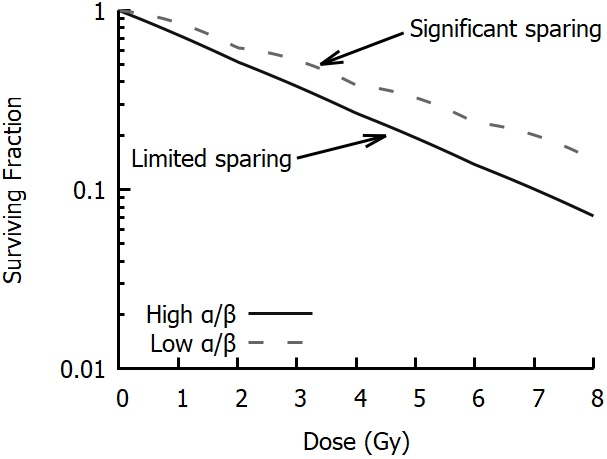
\includegraphics[width=0.9\linewidth]{sparing.jpg}
		\caption{Impatto del frazionamento. Nelle cellule con $\alpha/\beta=5\mbox{ Gy}$ dividere il trattamento in due frazioni da $2\mbox{ Gy}$ consente di risparmiare danni cellulari (sparing) modulando il contributo riparatore del fattore $\beta$: i danni cellulari vengono fortemente risparmiati nelle cellule caratterizzate da bassi $\alpha/\beta$ (cellule sane) mentre ciò non avviene nelle cellule con alti $\alpha/\beta$ (cellule tumorali) \cite{McMahon_2019}.}
		\label{fig:sparing}
	\end{figure}
	
	\section{Interazione della radiazione con la materia}
	Gli effetti biologici indotti dalla radiazione ionizzante sui tessuti e gli organi del corpo umano sono la manifestazione di interazioni elettromagnetiche e nucleari che avvengono a livello microscopico. Prima di descrivere le principali caratteristiche delle interazioni che interessano le cure radio e adroterapiche, si introduce il concetto di sezione d'urto che, in fisica nucleare e subnucleare, è un concetto indispensabile per la descrizione delle interazioni radiazione-materia. Successivamente, essendo i fotoni e le particelle cariche i protagonisti rispettivamente in radioterapia convenzionale e adroterapia, si analizzano in dettaglio le loro interazioni con la materia.
	
	\subsection{Sezione d'urto}\label{sec:sezione_urto}
	I fenomeni di interazione radiazione-materia, in cui onde o particelle\footnote{A livello quantistico sia la materia che la radiazione possiedono una duplice natura ondulatoria e corpuscolare, regolata dal principio di complementarità di Niels Bohr ($1885$--$1962$).} variano la loro traiettoria a seguito di processi di interazione e collisione, vengono descritti dagli esperimenti di diffusione (o scattering). Senza perdita di generalità, si utilizzerà un approccio classico per esporre lo schema tipico di un esperimento di diffusione, trattando le particelle come oggetti puntiformi.
	
	In un esperimento di scattering un fascio collimato di particelle proiettile $a$ di velocità $\vect{v_a}$ e sezione trasversale $A$ viene inviato da un acceleratore contro un bersaglio (o target) costituito da oggetti $b$ tutti uguali tra loro e distribuiti all'interno del volume del bersaglio stesso. Si suppone che le densità volumetriche del fascio $n_a$ e del bersaglio $n_b$ siano uniformi e costanti, che il target si presenti macroscopicamente come una lastra di spessore costante $\Delta z$ e che tutte le particelle proiettile, procedendo verso il bersaglio parallelamente alla direzione dell'asse $z$, lo colpiscano ortogonalmente (su una faccia di superficie $A$), come mostrato in \hyperref[fig:scattering]{Fig. 1.24}. Tali condizioni consentono di ricavare il numero di particelle incidenti sul target nell'unità di tempo $\phi_a$:
	\begin{equation}
		\frac{dN_a}{dt}=\phi_a=n_av_aA
		\label{eq:scattering1}
	\end{equation}
	Inoltre, il numero di centri diffusori $N_b$ (distribuiti nel volume del bersaglio intersecato dal fascio $V=A\Delta z$) con cui ogni particella proiettile può interagire è dato da:
	\begin{equation}
		N_b=n_bA\Delta z
		\label{eq:scattering2}
	\end{equation}
	\begin{figure}[H]
		\centering
		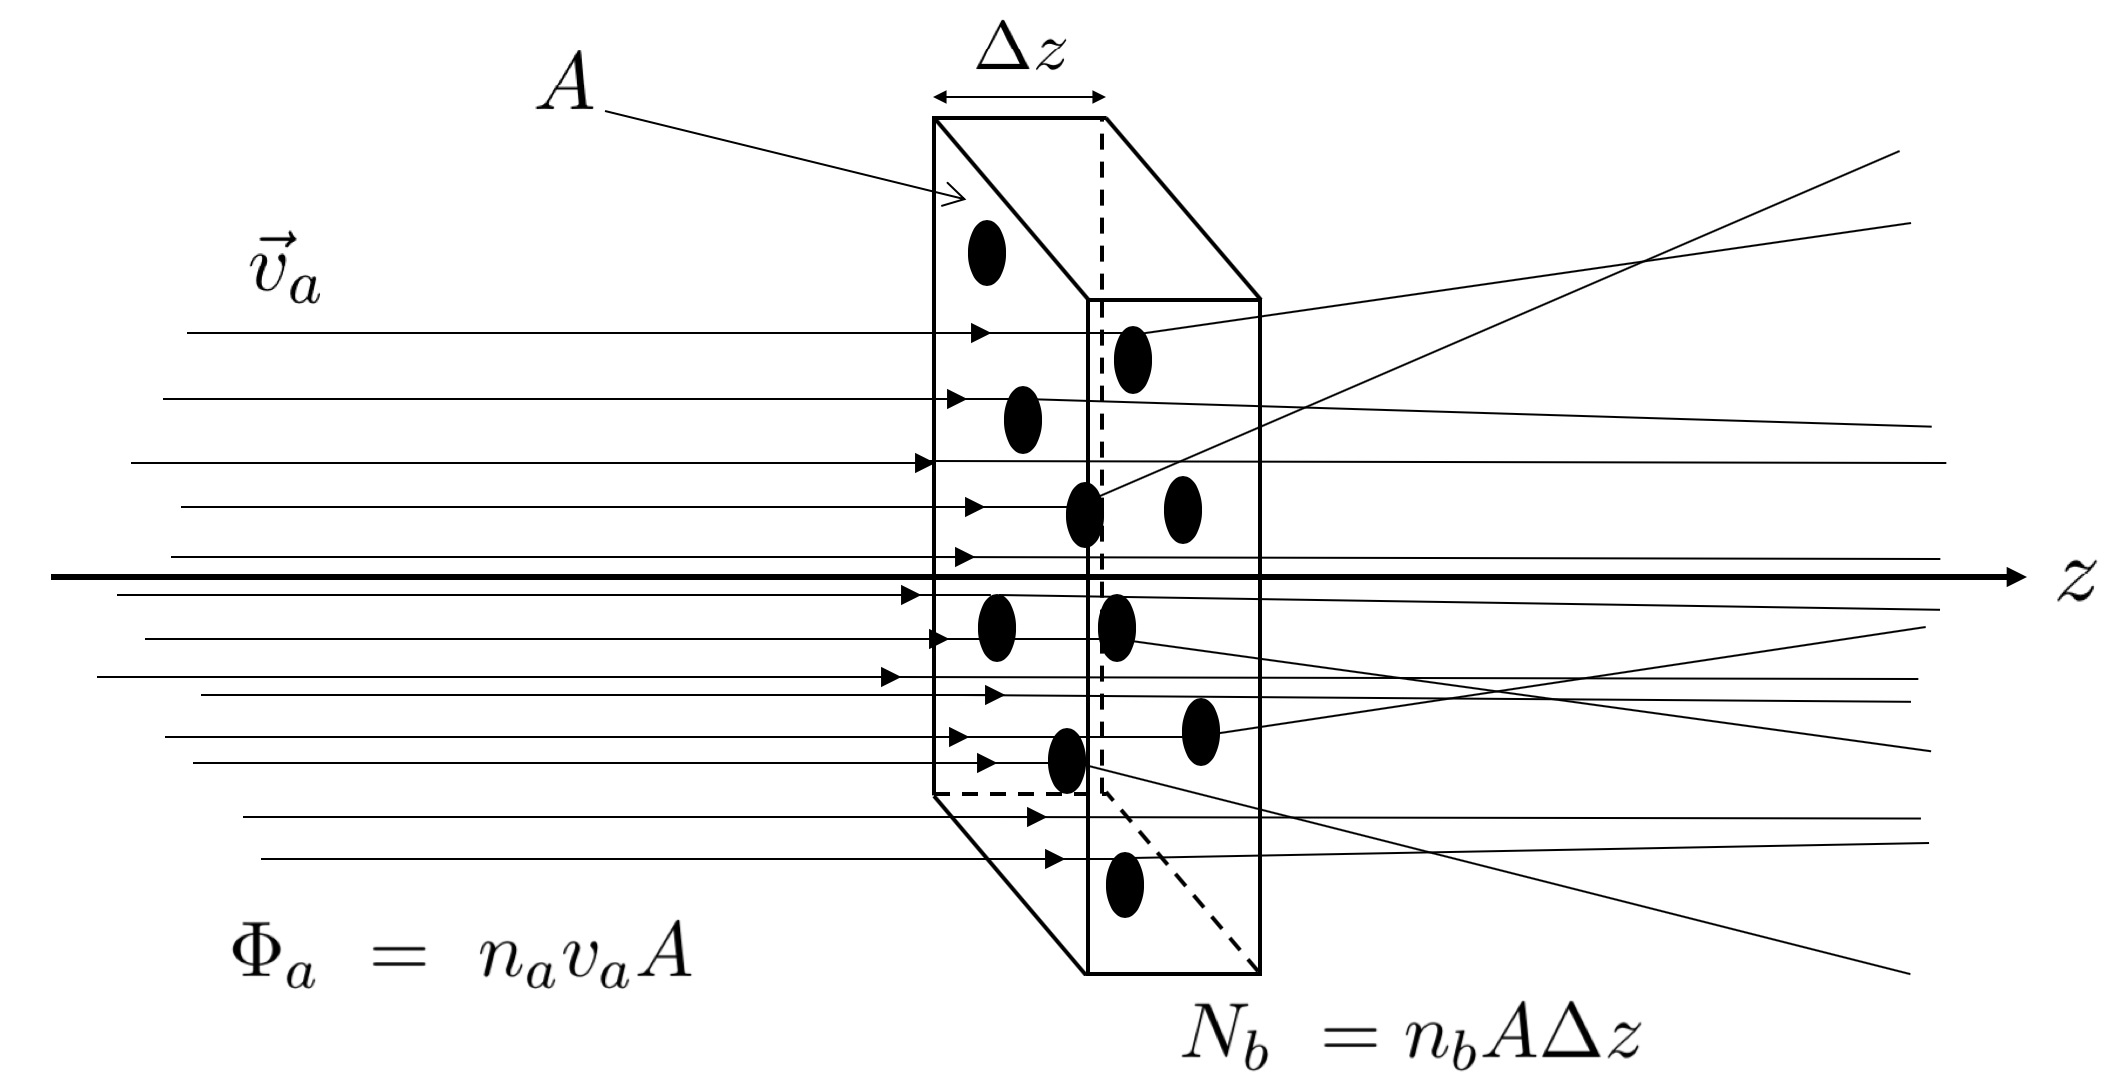
\includegraphics[width=0.9\linewidth]{scattering.jpg}
		\caption{Schema tipico di un esperimento di scattering \cite{units_sezUrto}.}
		\label{fig:scattering}
	\end{figure}
	Dato che ogni centro diffusore è caratterizzato da una sezione trasversale $\sigma_b$ (denominata sezione d'urto totale, indicata con dei cerchi pieni in \hyperref[fig:scattering]{Fig. 1.24}), la particella incidente effettua un'interazione con il bersaglio se la sua traiettoria interseca $\sigma_b$. Pertanto, la probabilità che una singola particella proiettile interagisca con una singola particella del bersaglio vale $\frac{\sigma_b}{A}$ che, unita alle \hyperref[eq:scattering1]{Eq. 1.18} ed \hyperref[eq:scattering2]{Eq. 1.19}, consente di ricavare il numero di particelle del fascio $\frac{dN}{dt}$ che, attraversando il target, interagiscono con esso nell'unità di tempo:
	\begin{equation}
		\frac{dN}{dt}=\frac{dN_a}{dt}\frac{\sigma_bN_b}{A}=n_an_bv_aA\sigma_b\Delta z
		\label{eq:scattering3}
	\end{equation}
	da cui, differenziando rispetto all'angolo solido $\Omega$, si ottiene la sezione d'urto differenziale $\frac{d\sigma_b}{d\Omega}$:
	\begin{equation}
		\frac{d\sigma_b}{d\Omega}=\frac{1}{\left(n_av_a\right)\left(n_bA\Delta z\right)}\frac{d}{d\Omega}\frac{dN_{\Delta\Omega}}{dt}
		\label{eq:scattering4}
	\end{equation}
	dove $\frac{d\sigma_b}{d\Omega}\Delta \Omega$ rappresenta la misura della probabilità che una particella venga diffusa entro l'angolo solido $\Delta \Omega$ e $\frac{dN_{\Delta\Omega}}{dt}$ è il numero di particelle deflesse dal target entro l'angolo $\Delta \Omega$ nell'unità di tempo (si veda \hyperref[fig:solid_angle]{Fig. 1.25}). Differenziando nuovamente la \hyperref[eq:scattering4]{Eq. 1.21} rispetto all'energia cinetica $E$, si ottiene la sezione d'urto doppiamente differenziale $\frac{d^2\sigma_b}{d\Omega dE}$:
	\begin{equation}
		\frac{d^2\sigma_b}{d\Omega dE}=\frac{1}{\left(n_av_a\right)\left(n_bA\Delta z\right)}\frac{d^2}{d\Omega dE}\frac{dN_{\Omega,\Delta E}}{dt}
		\label{eq:scattering5}
	\end{equation}
	dove $\frac{dN_{\Delta\Omega,\Delta E}}{dt}$ è il numero di particelle deflesse dal bersaglio entro l'angolo $\Delta \Omega$ con energia entro l'intervallo $\Delta E$ nell'unità di tempo.
	\begin{figure}[H]
		\centering
		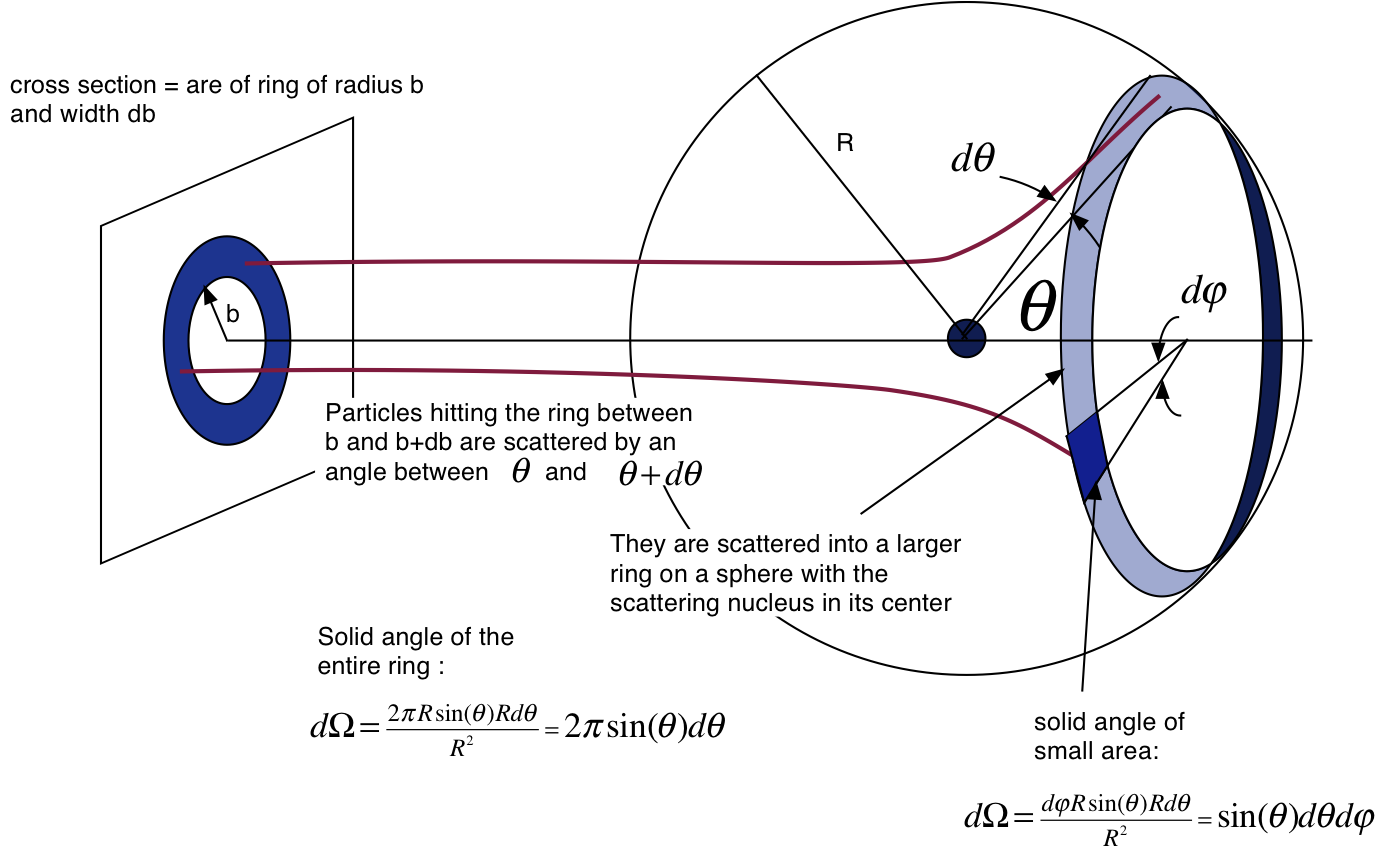
\includegraphics[width=0.9\linewidth]{solid_angle.png}
		\caption{Processo di scattering tridimensionale in cui le particelle passanti per la corona circolare (a sinistra) vengono diffuse da un centro scatteratore e indirizzate (a destra) nella corona sferica, descritta da un angolo solido \cite{wsuHarr}.}
		\label{fig:solid_angle}
	\end{figure}
	Riassumendo, la sezione d'urto è una quantità che misura la probabilità che una particella subisca un processo di scattering, con conseguente deflessione e eventuale perdita di energia. La sua importanza risiede nel fatto che riesce a collegare quantità microscopiche (come la sezione trasversale $\sigma_b$ della particella target) con quantità macroscopiche direttamente misurabili (come i parametri $n_a$, $n_b$, $A$, $\Delta z$ e $\frac{dN}{dt}$) \cite{sempriniNotes}.
	
	\subsection{Interazione dei fotoni con la materia}
	I fotoni (raggi $\gamma$) possono interagire con la materia nei seguenti modi:
	\begin{itemize}
		\item effetto fotoelettrico;
		\item scattering Compton;
		\item produzione di coppia;
		\item scattering Thomson and Rayleigh;
		\item reazioni fotonucleari.
	\end{itemize}
	Nei range energetici terapeutici (che vanno dal $\mbox{keV}$ al $\mbox{MeV}$) sia lo scattering Thomson and Rayleigh (in cui si verifica una diffusione elastica\footnote{Un processo di diffusione si definisce elastico se conserva l'energia cinetica del sistema.} a energie molto basse) che le reazioni fotonucleari (dove un raggio $\gamma$ con energia maggiore di $10\mbox{ MeV}$ colpisce un nucleo atomico emettendo protoni, neutroni e ioni) si possono trascurare. Le altre tre interazioni vengono analizzate nei paragrafi successivi.
	
	Innanzitutto, quando i fotoni attraversano la materia subiscono un processo di assorbimento\footnote{L'assorbimento del numero di fotoni $N(x)$ alla profondità $x$ coincide con l'attenuazione dell'intensità $I(x)$ del fascio fotonico essendo $I(x)=N(x)/(At)$, con $A$ e $t$ rispettivamente unità di superficie e di tempo.} descritto dalla legge di attenuazione di Lambert:
	\begin{equation}
		N(x)=N_0e^{-\mu x}
		\label{eq:lambert}
	\end{equation}
	dove $N_0$ è il numero di fotoni iniziali, $N(x)$ è il numero di fotoni alla profondità $x$ e $\mu$ è il coefficiente di attenuazione lineare, tale che $\left[\mu\right]=m^{-1}$. Chiaramente l'attenuazione del mezzo attraversato dal fotone risulta maggiore per alti valori di $\mu$. In generale, il coefficiente di attenuazione dipende sia dall'energia $E$ dei fotoni che dalla profondità $x$ (in quanto variando quest'ultima possono cambiare sia il tipo di materiale che il suo stato fisico), ma spesso è possibile ricavare un'espressione esplicita per $\mu$, riportata nella \hyperref[eq:attenuazione]{Eq. 1.24}:
	\begin{equation}
		\mu=n\sigma_{tot}=\frac{\rho N_A}{M_{mol}}\sigma_{tot}
		\label{eq:attenuazione}
	\end{equation}
	dove $n$ rappresenta il numero di centri diffusori per unità di volume e dipende dal numero di Avogadro $N_A$, dalla massa molecolare $M_{mol}$ e dalla densità del materiale attraversato $\rho$, mentre $\sigma_{tot}$ è la sezione d'urto totale e fornisce la probabilità totale di interazione del fotone con la materia; quest'ultima tiene conto dell'effetto cumulato di tutte le possibili interazioni fotone-materia rilevanti alle energie radioterapiche, quali l'effetto fotoelettrico, lo scattering Compton e la produzione di coppia \cite{testaNotes}:
	\begin{equation}
		\sigma_{tot}=\sigma_{fe}+\sigma_{C}+\sigma_{pc}
		\label{eq:sum_cross_section}
	\end{equation}
	dove $\sigma_{fe}$, $\sigma_{C}$ e $\sigma_{pc}$ sono rispettivamente le sezioni d'urto relative all'effetto fotoelettrico, allo scattering Compton e alla produzione di coppa. Pertanto, dalle \hyperref[eq:lambert]{Eq. 1.23}, \hyperref[eq:attenuazione]{Eq. 1.24} ed \hyperref[eq:sum_cross_section]{Eq. 1.25}, si ottiene la \hyperref[eq:photon_absorption]{Eq. 1.26} che riassume l'effetto di assorbimento che subisce un fotone nell'attraversare la materia:
	\begin{equation}
		N(x)=N_0e^{\frac{\rho N_A}{M_{mol}}}\cdot e^{-\sigma_{fe}x}\cdot e^{-\sigma_{C}x}\cdot e^{-\sigma_{pc}x}
		\label{eq:photon_absorption}
	\end{equation}
	
	\subsubsection{Effetto fotoelettrico}\label{par:effetto_fotoelettrico}
	L'interpretazione corretta dell'effetto fotoelettrico fu fornita da Albert Einstein ($1879$--$1955$) in uno dei suoi quattro articoli dell'\textit{Annus mirabilis}, pubblicato nel $1905$ \cite{Einstein1905-in}; tale scoperta gli valse il premio Nobel per la fisica nel $1921$.
	
	Nell'esperimento dell'effetto fotoelettrico proposto da Philipp von Lenard ($1862$--$1947$) si osserva che i metalli alcalini (come sodio \ce{Na}, litio \ce{Li} e potassio \ce{K}) acquistano una carica positiva quando vengono irradiati da fotoni caratterizzati da una bassa lunghezza d'onda. Dato che la materia è normalmente neutra, i metalli generano un'emissione di elettroni, essendo questi ultimi i portatori di carica negativa. \`E possibile spiegare l'effetto fotoelettrico osservando che i fotoni, colpendo gli elettroni appartenenti agli orbitali (o shell) più interni degli atomi metallici, vengono assorbiti; l'assorbimento dei fotoni comporta un processo anelastico\footnote{Un processo di diffusione si definisce anelastico se non conserva l'energia cinetica del sistema.} in cui l'energia trasportata dai fotoni viene trasformata in energia cinetica degli elettroni, che vengono dunque emessi dal metallo. Tale processo prende il nome di fotoemissione e gli elettroni emessi vengono denominati fotoelettroni \cite{zucchiniNotes}. L'energia del fotoelettrone $E_{e^-}$ è pari a:
	\begin{equation}
		E_{e^-}=E_\gamma-E_b=h\nu-E_b
		\label{eq:fotoelettrico}
	\end{equation}
	dove $E_\gamma$ e $\nu$ sono rispettivamente l'energia e la frequenza del fotone incidente, $h=6.626\cdot 10^{-34}\mbox{ Js}$ è la costante di Planck \cite{planckConstant}, e $E_b$ è l'energia di legame del fotoelettrone, che corrisponde all'energia che occorre fornire all'elettrone per slegarlo dall'atomo di metallo entro cui è contenuto (infatti $E_b$ è anche chiamato lavoro di estrazione). Il fotoelettrone, avendo liberato un posto nelle shell più interne agli atomi di metallo, genera una lacuna. Tale ``posto vacante'' viene successivamente riempito dagli elettroni che appartengono agli orbitali più esterni: a tale salto orbitale corrisponde una grande emissione di energia che in alcuni casi viene assorbita da altri elettroni (è il caso degli elettroni di Auger\footnote{Un elettrone di Auger, appartenendo all'orbitale più esterno dell'atomo, grazie all'energia ricevuta riesce ad essere liberato completamente.}), in altri può generare un raggio X, come illustrato in \hyperref[fig:fotoelettrico]{Fig. 1.26}.
	\begin{figure}[H]
		\centering
		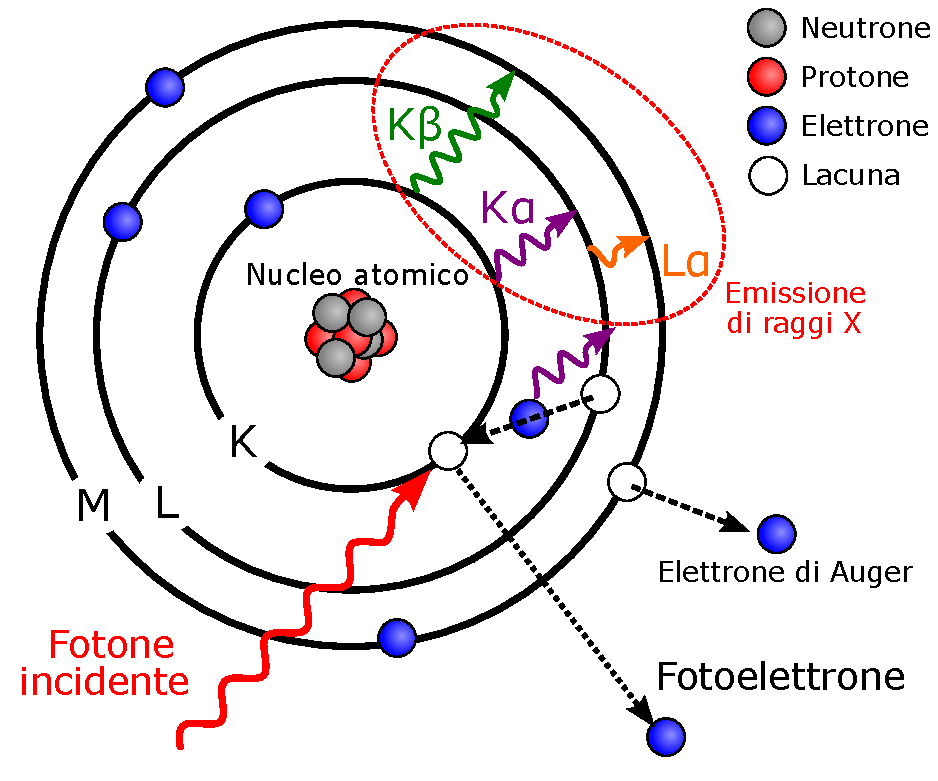
\includegraphics[width=0.8\linewidth]{fotoelettrico.pdf}
		\caption{Schema dell'effetto fotoelettrico e della conseguente emissione di raggi X o elettroni di Auger. Gli orbitali, indicati con notazione spettroscopica M, L e K, producono raggi X con le linee di emissione $K_\alpha$, $K_\beta$ e $L_\alpha$ \cite{ompInterations}.}
		\label{fig:fotoelettrico}
	\end{figure}
	\`E possibile ricavare l'andamento approssimativo della sezione d'urto dell'effetto fotoelettrico $\sigma_{fe}$ sia in funzione dell'energia del fotone $E_\gamma$ e del numero atomico $Z$ del bersaglio:
	\begin{equation}
		\sigma_{fe}\propto \frac{Z^4}{E^{\frac{7}{2}}_\gamma}
		\label{eq:sigma_fe1}
	\end{equation}
	sia in funzione dei numeri atomici $Z$ e di massa $A$ del target:
	\begin{equation}
		\sigma_{fe}\propto \frac{Z^5}{A}
		\label{eq:sigma_fe2}
	\end{equation}
	Dalla \hyperref[eq:sigma_fe1]{Eq. 1.28} si osserva che il contributo di $\sigma_{fe}$ diviene particolarmente importante per materiali dotati di atomi pesanti (con alto $Z$) e per basse $E_\gamma$.
	
	\subsubsection{Scattering Compton}
	L'interpretazione corretta dello scattering Compton valse al fisico statunitense Arthur Compton ($1892$--$1962$) il premio Nobel per la fisica nel $1927$.
	
	Nell'esperimento dello scattering Compton proposto dallo scienziato stesso, un fascio collimato di fotoni, caratterizzato da una frequenza approssimativamente monocromatica (che corrisponde a una lunghezza d'onda $\lambda_i$ appartenente allo spettro elettromagnetico dei raggi X), irradia un elettrone appartenente agli orbitali più esterni degli atomi di un blocco di grafite, attuando il processo di diffusione elastica mostrato in \hyperref[fig:compton]{Fig. 1.27}. A differenza dell'\hyperref[par:effetto_fotoelettrico]{effetto fotoelettrico}, si hanno due fotoni, uno prima e uno dopo l'interazione: il fotone incidente trasferisce quasi tutta la sua energia all'elettrone irradiato mentre il fotone diffuso, a causa del trasferimento di energia all'elettrone, possiede una minore frequenza del primo (che corrisponde a una maggiore lunghezza d'onda $\lambda_f$). Analizzando l'intensità della radiazione diffusa, Compton misurò lo shift in lunghezza d'onda $\Delta \lambda=\lambda_f-\lambda_i$ dei raggi X diffusi e incidenti (chiamato Compton shift), riuscendo a spiegare tale fenomeno imponendo la conservazione dell'energia e della quantità di moto dei fotoni e degli elettroni interagenti, ottenendo la \hyperref[eq:compton]{Eq. 1.30}:
	\begin{equation}
		\Delta \lambda=\frac{4\pi\hbar}{m_ec^2}\sin^2{\left(\frac{\theta}{2}\right)}
		\label{eq:compton}
	\end{equation}
	dove $\hbar=\frac{h}{2\pi}$ è la costante di Planck ridotta, $m_e=9.109\cdot^{-31}\mbox{ kg}$ è la massa dell'elettrone \cite{electronMass}, $c=2.998\cdot10^{8}\mbox{ m/s}$ è la velocità della luce nel vuoto \cite{soliv} e $\theta$ è l'angolo che intercorre tra la direzione del fotone incidente e quella del fotone diffuso.
	\begin{figure}[H]
		\centering
		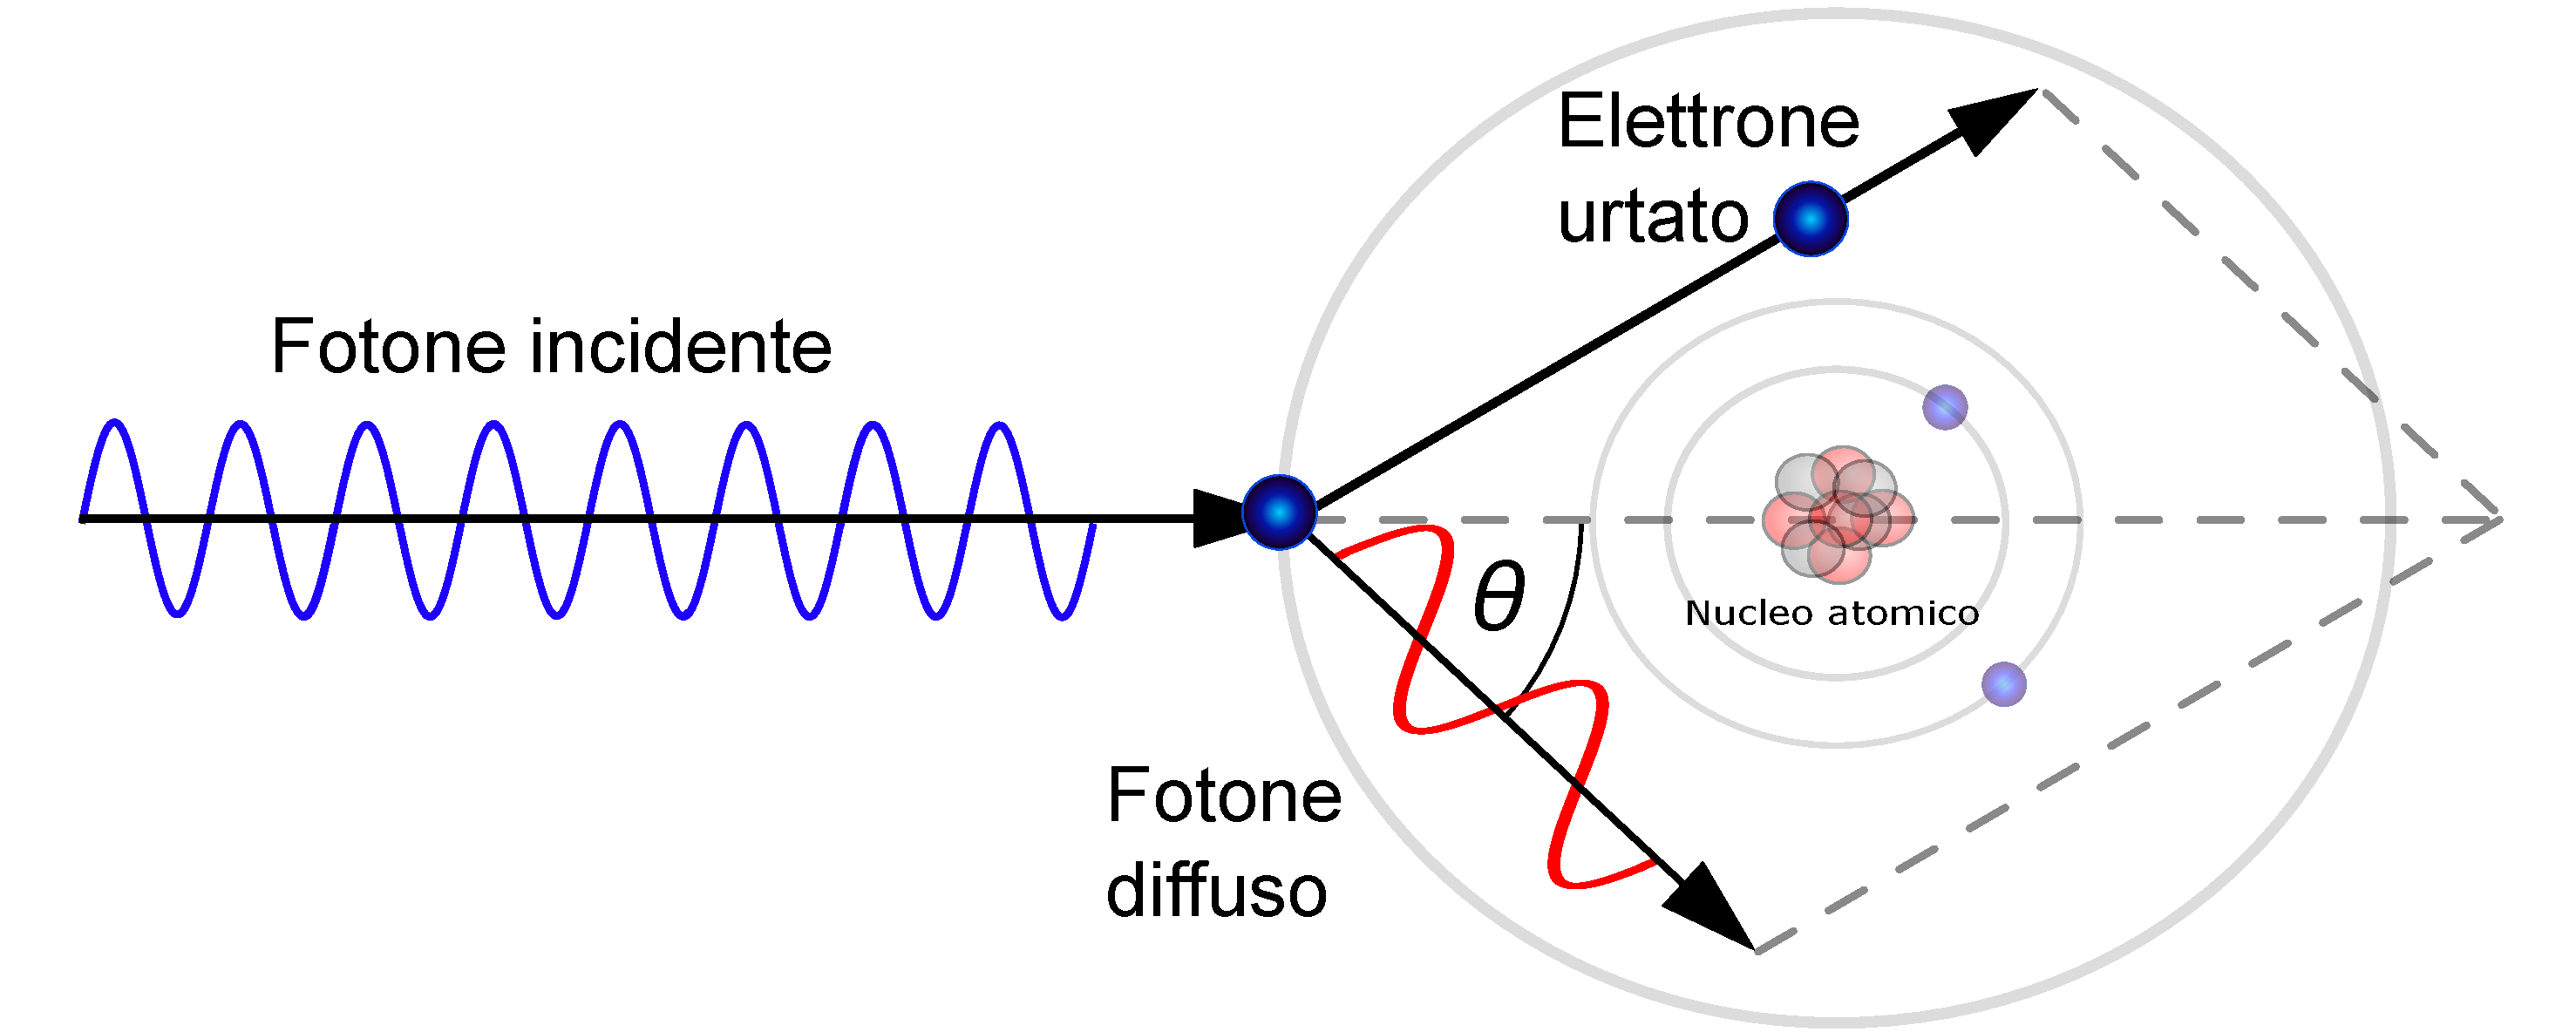
\includegraphics[width=0.9\linewidth]{compton.pdf}
		\caption{Schema dello scattering Compton \cite{comptScatt}.}
		\label{fig:compton}
	\end{figure}
	\`E possibile ricavare l'andamento approssimativo della sezione d'urto dello scattering Compton $\sigma_{C}$ sia in funzione dell'energia del fotone $E_\gamma$ e del numero atomico $Z$ del bersaglio:
	\begin{equation}
		\sigma_{C}\propto \frac{Z}{E_\gamma}
		\label{eq:sigma_c1}
	\end{equation}
	sia in funzione dei numeri atomici $Z$ e di massa $A$ del target:
	\begin{equation}
		\sigma_{C}\propto \frac{Z}{A}
		\label{eq:sigma_c2}
	\end{equation}
	Dalla \hyperref[eq:sigma_c1]{Eq. 1.31} si osserva che $\sigma_{C}$ viene attenuata linearmente all'aumentare di $E_\gamma$.
	
	\subsubsection{Produzione di coppia}
	La produzione di coppia è un processo di interazione elettromagnetica in cui un fotone, dotato di sufficiente energia ($E_\gamma>2m_e=1.022\mbox{ MeV}$), trasforma tutta la sua energia in massa producendo un elettrone e un positrone secondo il diagramma di Feynman riportato in \hyperref[fig:feynman]{Fig. 1.28}:
	\begin{figure}
		\centering
		\begin{tikzpicture}
			\begin{feynman}[large]
				\vertex (a);
				\vertex [right=of a] (b);
				\vertex [above right=of b] (f1) {$e^-$};
				\vertex [below right=of b] (f2) {$e^+$};
				\diagram* {
					(a) -- [photon, edge label'=$\gamma$] (b) -- [fermion] (f1),
					(b) -- [anti fermion] (f2),
				};
			\end{feynman}
		\end{tikzpicture}
		\caption{Diagramma di Feynman della produzione di coppia elettrone-positrone.}
		\label{fig:feynman}
	\end{figure}
	Non è possibile giustificare tale interazione con le leggi dell'elettromagnetismo classico, ma è necessario il supporto di teorie di campo quantizzato\footnote{In particolare, si fa riferimento all'elettrodinamica quantistica o QED.} con le quali si può interpretare la trasformazione di energia in materia (e antimateria) che ha luogo durante il processo. La produzione di coppia elettrone-positrone da parte di un fotone avviene solo se quest'ultimo interagisce con un altro corpo (in questo caso o il nucleo atomico o un elettrone, che interagiscono con il fotone per interazione coulombiana; la presenza di un forte campo elettrico è infatti necessaria per consentire la conversione di energia in massa), altrimenti si violerebbe la conservazione del quadrimpulso.\footnote{Nel contesto relativistico la conservazione del quadrimpulso è una generalizzazione della conservazione di energia e quantità di moto.}
	
	Durante la produzione di coppia, l'energia del fotone si ripartisce equamente nell'elettrone e nel positrone ma, successivamente, gli esiti delle due particelle materiali sono differenti: l'elettrone perde energia cinetica generando eventi di ionizzazione mentre il positrone si annichila\footnote{L'annichilazione è il processo inverso alla produzione di coppia in cui un elettrone e un positrone si trasformano in due raggi $\gamma$, convertendo totalmente la loro massa in energia.} con un alto elettrone, producendo due raggi $\gamma$ in direzioni antiparallele (la produzione di un solo raggio $\gamma$ sarebbe impedita dalla conservazione del quadrimpulso), come mostrato in \hyperref[fig:pair_production]{Fig. 1.29}.
	\begin{figure}[H]
		\centering
		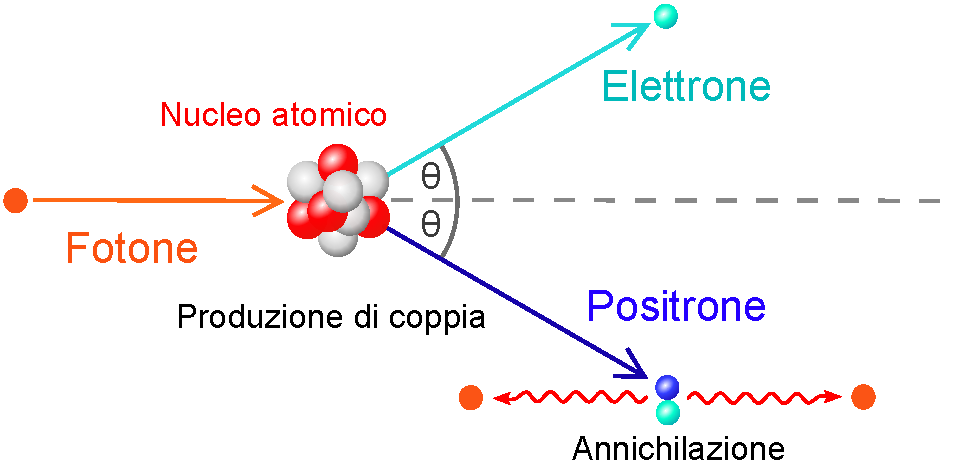
\includegraphics[width=0.9\linewidth]{pair_production.pdf}
		\caption{Schema della produzione di coppia e successiva annichilazione elettrone-positrone \cite{pairProd}.}
		\label{fig:pair_production}
	\end{figure}
	Dai diagrammi di Feynman è possibile ricavare l'andamento approssimativo della sezione d'urto della produzione di coppia $\sigma_{pc}$ sia in funzione dell'energia del fotone $E_\gamma$ e del numero atomico $Z$ del bersaglio:
	\begin{equation}
		\sigma_{pc}\propto \frac{Z^2}{\ln{E_\gamma}}
		\label{eq:sigma_pc1}
	\end{equation}
	sia in funzione dei numeri atomici $Z$ e di massa $A$ del target:
	\begin{equation}
		\sigma_{pc}\propto \frac{Z^2}{A}
		\label{eq:sigma_pc2}
	\end{equation}
	Dalla \hyperref[eq:sigma_pc1]{Eq. 1.33} si osserva che $\sigma_{pc}$ è sostanzialmente costante per alte $E_\gamma$.	
	
	La \hyperref[fig:attenuation]{Fig. 1.30} riassume l'andamento della sezione d'urto totale per unità di massa dell'interazione fotone-materia. Si osserva che per basse energie domina l'effetto fotoelettrico, per energie dell'ordine di $1\mbox{ MeV}$ prevale lo scattering Compton e per energie dell'ordine di $10\mbox{ MeV}$ (e maggiori) dominano lo scattering Compton e la produzione di coppia.
	\begin{figure}[H]
		\centering
		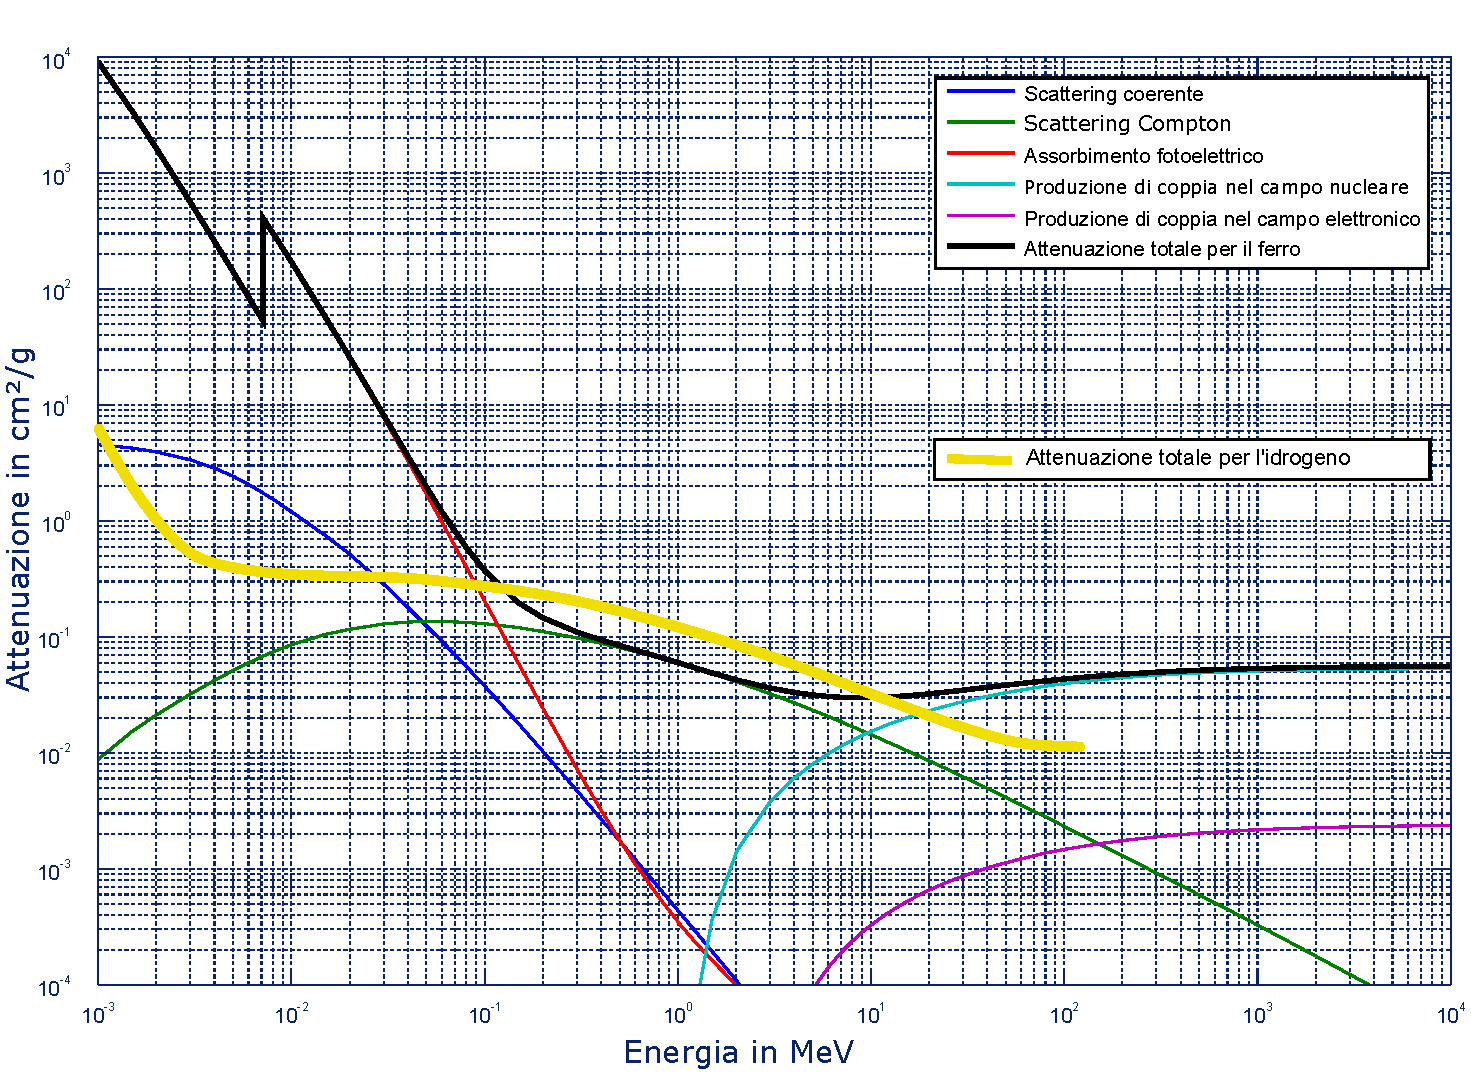
\includegraphics[width=0.9\linewidth]{attenuation.pdf}
		\caption{Andamento della sezione d'urto totale (attenuazione) per unità di massa in funzione dell'energia del fotone incidente in un materiale di ferro e di idrogeno, rappresentati in una scala doppio-logaritmica. Per scattering coerente si intende un tipo di scattering in cui il fotone incidente e quello diffuso possiedono la stessa lunghezza d'onda (è un effetto Compton con $\Delta \lambda=0$). Al centro del grafico si evidenzia il range energetico radioterapico \cite{attenCoeff,Marghany2021-xg}.}
		\label{fig:attenuation}
	\end{figure}
	Essendo il corpo umano principalmente formato da acqua, l'analisi della sezione d'urto totale dell'interazione fotone-acqua risulta essere una buona approssimazione delle interazioni che intercorrono tra i raggi $\gamma$ e il corpo umano durante la radioterapia. Tale situazione viene illustrata in \hyperref[fig:attenuation_water]{Fig. 1.31}, dove è evidente la diminuzione esponenziale della sezione d'urto all'aumentare dell'energia. Ciò avviene perché aumentando l'energia dei raggi $\gamma$ incidenti diminuisce l'effetto attenuativo svolto dall'acqua, che consente al fotone di penetrare maggiormente all'interno del bersaglio; quindi, una maggiore penetrazione è legata a una diminuzione degli eventi di interazione fotone-acqua (ossia a un abbassamento della sezione d'urto).
	\begin{figure}[H]
		\centering
		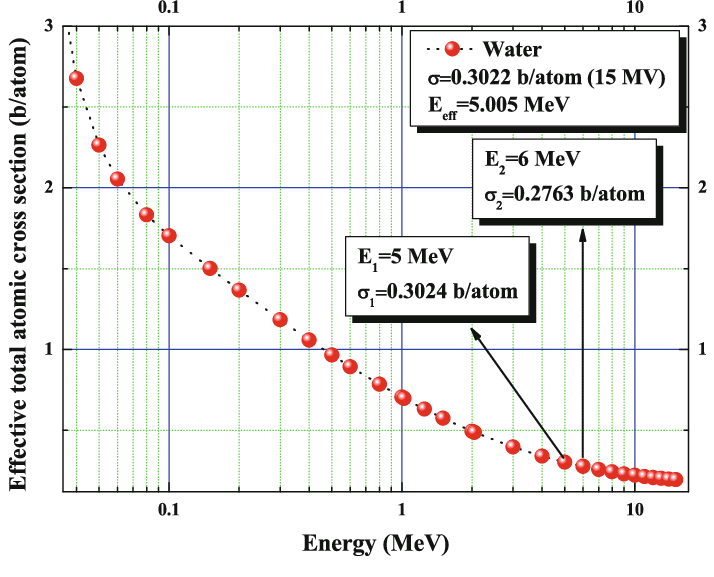
\includegraphics[width=0.9\linewidth]{attenuation_water.png}
		\caption{Andamento della sezione d'urto efficace in funzione dell'energia del fotone incidente in acqua. Si ricorda che il barn (b) è un'unità di misura di superficie tale che $1\mbox{ b}=10^{-24}\mbox{ cm}^{2}$ \cite{muratRadiation}.}
		\label{fig:attenuation_water}
	\end{figure}
	
	\subsection{Interazione delle particelle cariche con la materia}
	Le particelle cariche interagiscono con la materia in modo più complesso rispetto ai fotoni. Ad esempio, quando le particelle cariche attraversano la materia perdono energia fino ad arrestarsi, un fenomeno che non riguarda i fotoni che, quando interagiscono, possono essere solamente emessi o assorbiti. Inoltre, le interazioni effettuate dalle particelle cariche sono sia di tipo elettromagnetico che nucleare. In particolare, i processi elettromagnetici sono descritti dalle seguenti interazioni:
	\begin{itemize}
		\item Bethe-Bloch, che avviene con gli elettroni atomici del bersaglio attraverso processi di diffusione anelastici;
		\item scattering Rutherford (o scattering multiplo coulombiano), che avviene con il nucleo del bersaglio attraverso processi di diffusione elastici;
		\item bremsstrahlung (o radiazione di frenamento), che avviene con il nucleo del bersaglio;
		\item effetto Cherenkov, che avviene con gli elettroni atomici e con il nucleo del bersaglio.
	\end{itemize}
	L'interazione elettromagnetica delle particelle cariche con gli elettroni atomici domina sia rispetto alle interazioni nucleari sia rispetto all'interazione elettromagnetica con in nuclei per via delle dimensioni lineari dell'atomo e del suo nucleo. Infatti, essendo l'atomo $10^4$ volte più grande (linearmente) del nucleo, si ha che la sezione d'urto dei processi atomici $\sigma_{atom}$ è più grande di un fattore $10^8$ rispetto alla sezione d'urto che descrive le interazioni nucleari $\sigma_{nucl}$; in particolare, i valori delle sezioni d'urto sono $\sigma_{atom}=100\mbox{ Mb}$ e $\sigma_{nucl}=1\mbox{ b}$. Il grande valore di $\sigma_{atom}$ testimonia l'elevatissimo numero di collisioni effettuate tra particelle cariche ed elettroni atomici, che renderebbe vana una trattazione analitica dell'interazione elettromagnetica basata sul calcolo delle sezioni d'urto. Quindi, si procede con un approccio energetico in cui si analizza la quantità di energia ceduta dalle particelle cariche durante il loro moto all'interno della materia.
	
	\subsubsection{Bethe-Bloch}\label{par:bethe_bloch}
	Quando una particella carica si muove in un mezzo materiale, esercita una forza sugli elettroni atomici del bersaglio che portano a numerosi processi di ionizzazione \cite{Christodoulides2016}. Il tasso di energia media persa\footnote{A causa degli eventi di ionizzazione.} per unità di lunghezza lungo il percorso da una particella carica è dato dalla formula relativistica di Bethe-Bloch (o del potere frenante), riportata in \hyperref[eq:bethe_bloch]{Eq. 1.35}:
	\begin{equation}
		\begin{split}
			\left\langle-\frac{dE}{dx} \right\rangle=\frac{\rho Z}{A}\frac{4\pi N_Am_ec^2}{M_U}&\left(\frac{e^2}{4\pi\epsilon_0m_ec^2}\right)^2\cdot\\
			&\cdot\frac{z^2}{\beta^2}\left[\ln{\left(\frac{2m_ec^2\beta^2}{I\left(1-\beta^2\right)}\right)}-\beta^2-\frac{\delta}{2}-\frac{C}{Z}\right]
		\end{split}
		\label{eq:bethe_bloch}
	\end{equation}
	i cui parametri sono riassunti in \hyperref[tab:bethe_bloch]{Tab. 1.3}; si notino sia il segno negativo in $\left\langle-\frac{dE}{dx} \right\rangle$ (che rappresenta la perdita di energia della particella carica) sia l'andamento quadratico rispetto al numero atomico delle particelle del fascio $z$.
	\begin{table}[H]
		\begin{minipage}{\textwidth}
			\centering
			\begin{tabular}{ |M{2cm}||m{10cm}| }
				\hline
				\multicolumn{2}{|c|}{Proprietà del mezzo}\\
				\hline\hline
				$\rho$ & Densità del materiale \\
				\hline
				$Z$ & Numero atomico\\
				\hline
				$A$ & Numero di massa\\
				\hline
				$I$ & Potenziale di ionizzazione\\
				\hline\hline
				\multicolumn{2}{|c|}{Costanti}\\
				\hline\hline
				$N_A$ & Numero di Avogadro\\
				\hline\hline
				$m_e$ & Massa dell'elettrone\\
				\hline
				$M_U$ & Massa molare ($\frac{1}{12}$ della massa di \ce{^{12}C}) \\
				\hline
				$\epsilon_0$ & Costante dielettrica nel vuoto\\
				\hline
				$e$ & Carica dell'elettrone\\
				\hline
				$c$ & Velocità della luce nel vuoto\\
				\hline\hline
				\multicolumn{2}{|c|}{Caratteristiche del fascio}\\
				\hline\hline
				$z$ & Numero atomico delle particelle del fascio\\
				\hline
				$\beta$ & Velocità del fascio in unità di $c$\\
				\hline\hline
				\multicolumn{2}{|c|}{Correzioni}\\
				\hline\hline
				$\delta$ & Correzione di densità, importante per alte energie\\
				\hline
				$C$ & Correzione di shell, importante per basse energie\\
				\hline
			\end{tabular}
		\end{minipage}
		\caption{Tabella riassuntiva dei parametri della Bethe-Bloch suddivisi in proprietà del mezzo, costanti, caratteristiche del fascio e correzioni. Solitamente nei range adroterapici si ha $Z/A$$\approx0.42$--$0.5$ e $I\approx19$--$820\mbox{ eV}$.}
		\label{tab:bethe_bloch}
	\end{table}
	I processi di interazione descritti dalla Bethe-Bloch sono stocastici: se $n$ particelle identiche aventi tutte la stessa energia iniziale attraversassero un'identica porzione di materiale, in generale subirebbero perdite di energia differenti. La formula di Bethe-Bloch fornisce il valore medio di tali perdite di energia, ma la natura statistica delle stesse ne consente una descrizione più approfondita tramite distribuzioni di probabilità. Ad esempio, se le particelle attraversassero strati sottili di materiali a bassa densità le fluttuazioni delle perdite di energia per unità di lunghezza sarebbero ben descritte da una distribuzione di Landau, altrimenti per spessi strati di materia ad alta densità la distribuzione sarebbe sostanzialmente Gaussiana (a causa del maggiore numero di collisioni che consente l'applicazione del teorema del limite centrale) \cite{bortolettoLecture,betheFormula}.
	
	\`E possibile suddividere l'andamento della Bethe-Bloch (mostrato in \hyperref[fig:bethe_bloch]{Fig. 1.32}) in varie regioni \cite{Christodoulides2016}:
	\begin{itemize}
		\item per energie molto basse l'energia cinetica della particella incidente viene corretta dal fattore $C$ (correzione di shell) in \hyperref[eq:bethe_bloch]{Eq. 1.35} che include effetti energetici dovuti al moto dell'elettrone attorno al nucleo. In questa regione vi sono anche altre correzioni minori come l'effetto Barkas, che tiene conto degli effetti coulombiani causati dalla carica della particella proiettile.
		\item Regione classica: per basse energie ($\beta\gamma<1$)\footnote{$\gamma=1/\sqrt{1-\beta^2}$ è denominato fattore di Lorentz.} il potere frenante diminuisce come $\frac{1}{\beta^2}$ in quanto le particelle cariche più veloci passano meno tempo nelle vicinanze degli atomi della materia, pertanto generano meno processi di ionizzazione.
		\item Regione di minima ionizzazione: per energie più alte ($\beta\gamma\approx3$) si osserva un minimo di ionizzazione dipendente da $\beta$ e (quasi) indipendente dalla massa della particella carica.
		\item Regione relativistica: per alte energie ($\beta\gamma>4$) si osserva una risalita logaritmica del potere frenante dovuta alla concentrazione delle linee di campo elettrico nella direzione ortogonale alla velocità della particella incidente, un effetto puramente relativistico. L'andamento di tale regione è dato dal termine logaritmico in \hyperref[eq:bethe_bloch]{Eq. 1.35}.
		\item Per energie molto alte la concentrazione delle linee di campo elettrico induce eventi di ionizzazione anche su atomi molto distanti dalla sua traiettoria; ciò provoca una polarizzazione negli atomi più distanti che produce un effetto di schermatura del campo elettrico stesso (definito effetto densità), che a sua volta determina il troncamento della risalita relativistica. L'effetto densità è controllato dal fattore $\delta$ (correzione di densità) in \hyperref[eq:bethe_bloch]{Eq. 1.35}.
	\end{itemize}
	\begin{figure}[H]
		\centering
		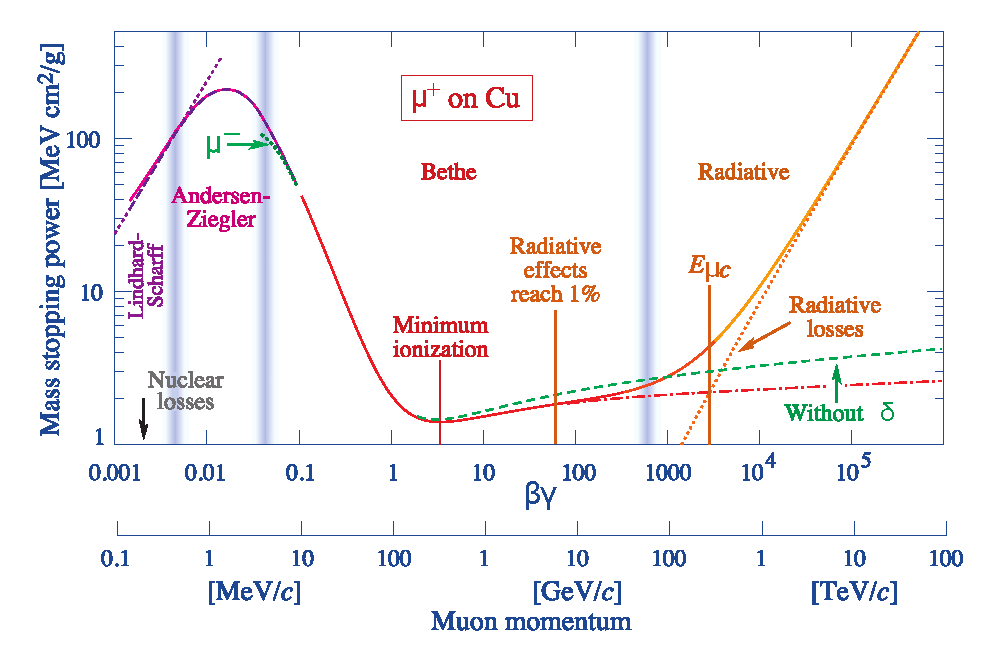
\includegraphics[width=0.9\linewidth]{bethe_bloch.pdf}
		\caption{Valore assoluto del potere frenante per $\mu^+$ in rame in funzione di $\beta\gamma=p/Mc$, dove $p$ è il modulo della quantità di moto relativistica del $\mu^+$. Le bande verticali delimitano varie regioni di approssimazione, alcune delle quali sono discusse nel testo. In particolare, la linea verde tratteggiata indicata con $\mu^+$ tiene conto dell'effetto Barkas mentre la linea rossa tratteggiata rappresenta l'azione dell'effetto densità \cite{groomPassage}.}
		\label{fig:bethe_bloch}
	\end{figure}
	In \hyperref[fig:adroterapic_range]{Fig. 1.33} viene riportato il potere frenante di un protone per energie molto basse, corrispondenti al range utilizzato in adroterapia. Entrambe le \hyperref[fig:bethe_bloch]{Fig. 1.32} e \hyperref[fig:adroterapic_range]{Fig. 1.33} mostrano che il maggior rilascio di energia della particella carica si ha per basse velocità (testimoniato anche dall'andamento $\frac{1}{\beta^2}$ della regione classica). In altre parole, le particelle cariche rilasciano la quasi totalità della loro energia al termine del loro percorso in uno spazio lineare piuttosto ristretto; tale peculiarità ha incoraggiato il loro impiego in adroterapia. A tale scopo si definisce il range $R$, ossia la profondità alla quale metà delle particelle cariche penetrate si fermano, definito come:
	\begin{equation}
		R(E_{tot})=\int_{m_0c^2}^{E_{tot}}\frac{dE}{\left(\frac{dE}{dx}\right)}
		\label{eq:range}
	\end{equation}
	dove $m_0$ e $E_{tot}$ sono rispettivamente la massa a riposo e l'energia totale della particella incidente e le altre sono costanti già descritte in \hyperref[tab:bethe_bloch]{Tab. 1.3}. Il range si ottiene integrando il potere frenante fornito dalla \hyperref[eq:bethe_bloch]{Eq. 1.35} su tutto il range energetico rilasciato, calcolo molto complicato vista la complessità della Bethe-Bloch. In generale è possibile approssimare la \hyperref[eq:range]{Eq. 1.36} con una relazione molto utile in adroterapia:
	\begin{equation}
		R(E_{tot})=\alpha E_{tot}^p
		\label{eq:range_approx}
	\end{equation}
	dove $\alpha$ e $p$ sono parametri dipendenti rispettivamente dal bersaglio e dall'energia. Essendo la Bethe-Bloch una legge statistica, le particelle appartenenti a un certo fascio possono potrebbero possedere valori di range caratterizzati da piccole fluttuazioni, conosciute come ``range straggling''; ciò risulterebbe problematico in adroterapia nel momento in cui si volessero risparmiare delle regioni tissutali sane nelle vicinanze di un tumore. \`E possibile ricavare che l'incidenza delle fluttuazioni nel range è piuttosto ridotta: ad esempio, irradiando un protone a $200\mbox{ MeV}$ in acqua si ha $R=25.8\mbox{ cm}$ con fluttuazioni di $2.5\mbox{ mm}$ (pari all $1\%$ circa).
	\begin{figure}[H]
		\centering
		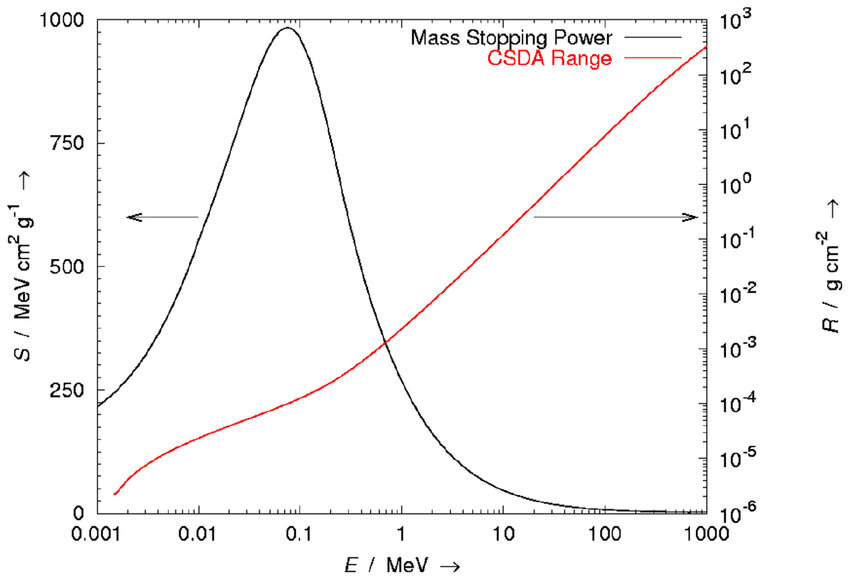
\includegraphics[width=0.9\linewidth]{adroterapic_range.png}
		\caption{Andamento del potere frenante e del range in funzione dell'energia di un protone in acqua \cite{NewhauserArticle}.}
		\label{fig:adroterapic_range}
	\end{figure}
	
	\subsubsection{Scattering Rutherford, Bremsstrahlung ed effetto Cherenkov}\label{par:scattering_Rutherford}
	Nello scattering Rutherford una particella carica viene deflessa a causa delle interazioni elettromagnetiche multiple indotte dai campi coulombiani dei nuclei del bersaglio. Per via dell'elasticità del processo, ciò che contraddistingue lo scattering Rutherford non è la variazione di energia della particella incidente ma il suo angolo di deflessione a valle dei processi di diffusione multipli, come illustrato in \hyperref[fig:rutherford_scattering]{Fig. 1.34}. Se l'interazione delle particelle cariche con gli elettroni portava a un range straggling longitudinale,\footnote{Per longitudinale si intende parallelo alla direzione del fascio incidente.} l'interazione delle stesse con i nuclei atomici induce fluttuazioni laterali, da considerare nel TP del paziente. Riportando l'esempio dell'irradiazione di un protone a $200\mbox{ MeV}$ in acqua, si hanno fluttuazioni laterali di di $5\mbox{ mm}$ (pari all $2\%$ circa).
	\begin{figure}[H]
		\centering
		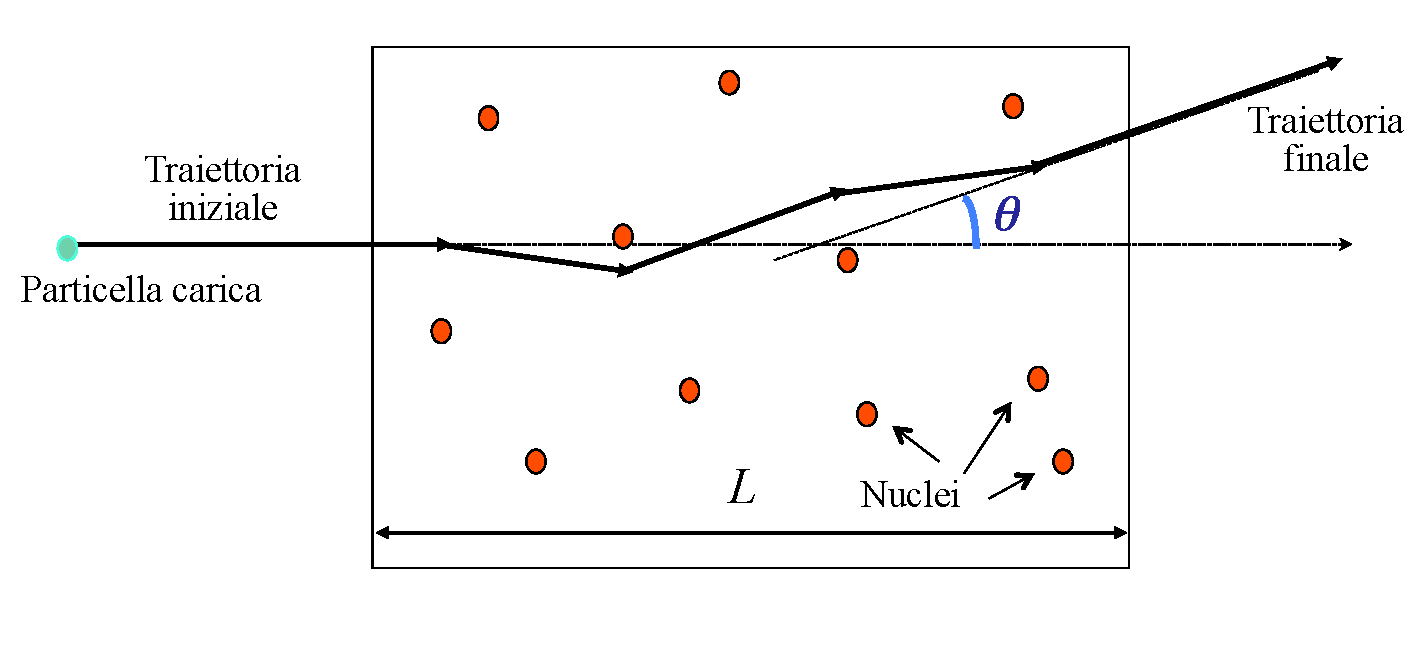
\includegraphics[width=0.9\linewidth]{rutherford_scattering.pdf}
		\caption{Schema dello scattering Rutherford di una particella carica in un mezzo di spessore $L$ \cite{batignaniNotes}.}
		\label{fig:rutherford_scattering}
	\end{figure}
	Per determinare la probabilità di interazione per scattering Rutherford si utilizza la sezione d'urto differenziale del processo, riportata in \hyperref[eq:rutherford_scattering]{Eq. 1.38}:
	\begin{equation}
		\frac{d\sigma}{d\Omega}=\left(\frac{1}{4\pi\epsilon_0}\frac{Z_1Z_2e^2}{4E_0}\right)^2\frac{1}{\sin^4{\frac{\theta}{2}}}
		\label{eq:rutherford_scattering}
	\end{equation}
	dove $\theta$ è l'angolo di deflessione della particella incidente, $E_0$ è la sua energia, $Z_1$ e $Z_2$ sono rispettivamente il numero atomico della particella incidente e del bersaglio e le altre sono costanti già descritte in \hyperref[tab:bethe_bloch]{Tab. 1.3}.
	
	I contributi apportati dalla Bremsstrahlung (``radiazione di frenamento'')\footnote{Nella Bremsstrahlung le particelle cariche decelerano a causa dell'interazione con il campo elettrico coulombiano del nucleo, perdendo energia ed emettendo una distribuzione continua di radiazione \cite{testaNotes}.} e dall'effetto Cherenkov\footnote{Quando una particella carica si muove in un mezzo con una velocità maggiore della velocità della luce nello stesso mezzo, emette radiazione elettromagnetica.} risultano trascurabili rispetto alle interazioni descritte nei paragrafi precedenti. In particolare, la Bremsstrahlung risulta trascurabile per le particelle pesanti (come ioni, particelle $\alpha$ e ioni pesanti) in quanto a basse energie $\left(-\frac{dE}{dx}\right)_{Brem}\propto\frac{Z^2}{m^2}$ (dove $Z$ è il numero atomico del target e $m$ è la massa delle particelle proiettile) e l'effetto Cherenkov risulta trascurabile in quanto si verifica per indici di rifrazione del bersaglio $n>0.75$, mentre l'indice di rifrazione del corpo umano (paragonabile a quello dell'acqua) è $n_{acqua}=1.33$.
	
	Riassumendo, le particelle cariche effettuano interazioni elettromagnetiche principalmente con gli atomi elettronici del bersaglio nelle modalità descritte dalla \hyperref[par:bethe_bloch]{Bethe-Bloch} e, in secondo luogo, con i nuclei degli atomi del target tramite \hyperref[par:scattering_Rutherford]{scattering Rutherford}. Come già anticipato nell'analisi della \hyperref[fig:bethe_bloch]{Fig. 1.32}, le particelle cariche perdono la maggior parte della loro energia a bassa velocità, negli istanti di tempo precedenti al loro arresto all'interno del materiale; ciò genera il già citato picco di Bragg, a cui corrisponde un massimo dell'energia rilasciata durante la penetrazione nel bersaglio. Mentre il profilo di dose di particelle cariche pesanti come protoni e ioni carbonio è caratterizzato dal BP, ciò non avviene nel caso dei fotoni (la cui energia viene rilasciata tramite un'attenuazione esponenziale) a causa dei suoi differenti processi di interazione con la materia. Come evidenziato in \hyperref[fig:photon]{Fig. 1.17}, la presenza del BP nel profilo di dose permette un migliore controllo dell'energia depositata nei tessuti del corpo umano, garantendo un'efficienza migliore nella cura dei tumori.
	
	La forte dipendenza della profondità a cui si verifica il picco di Bragg dall'energia del fascio incidente (si veda \hyperref[fig:bragg_peak_energies]{Fig. 1.35a}) suggerisce che una corretta scelta di quest'ultima possa far corrispondere il volume tumorale presente nel tessuto del paziente con il picco di Bragg, in modo che il maggiore rilascio di dose avvenga proprio nella regione cancerosa. Tuttavia, spesso accade che la larghezza del BP (pari a $2.5\mbox{ mm}$ per un fascio di protoni a $200\mbox{ MeV}$ in acqua) non è sufficiente a ricoprire l'intero volume tumorale,\footnote{In generale, un solo BP non è in grado di ricoprire la struttura tridimensionale di un tumore.} per questo si procede con il SOBP (Spread Out Bragg Peak), tecnica in cui si forniscono più fasci di particelle a diverse energie per generare un picco di Bragg ``allargato'' (si veda \hyperref[fig:sobp]{Fig. 1.35b}). Chiaramente l'inviluppo degli effetti si ha non solo in corrispondenza della regione tumorale ma anche nel canale di ingresso o subito dopo il BP; nonostante ciò, dalla \hyperref[fig:critical_organ]{Fig. 1.35c}, si osserva come l'adroterapia consenta un risparmio maggiore dei tessuti sani rispetto alla radioterapia convenzionale.
		\begin{figure}[H]
		\centering
		\begin{subfigure}[t]{0.49\textwidth}
			\centering
			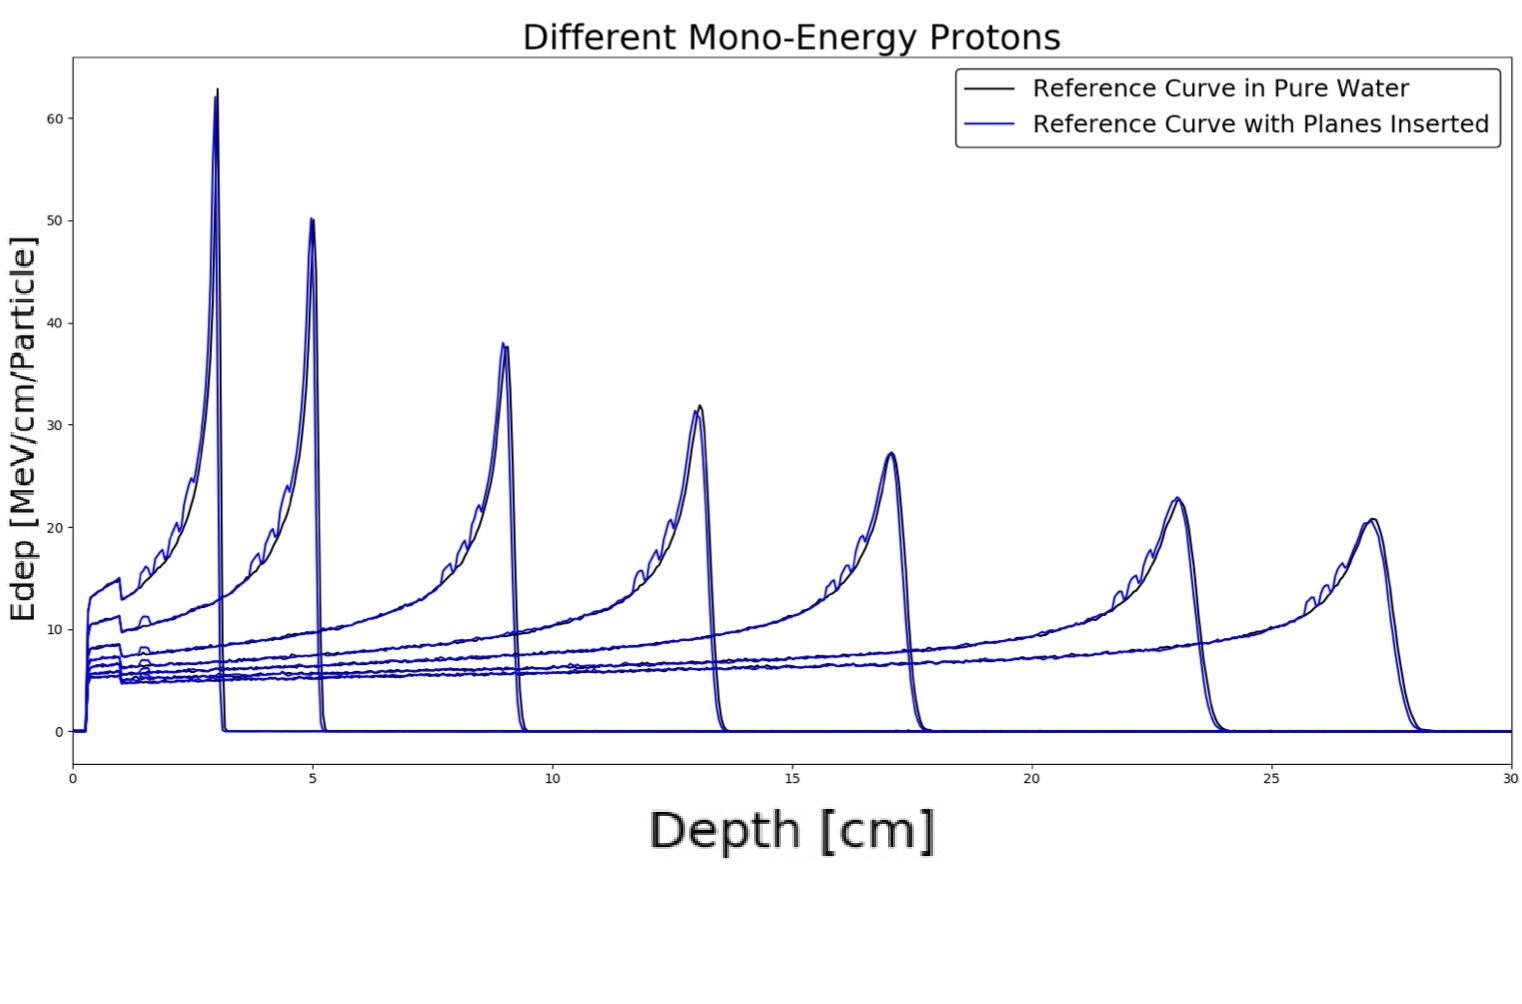
\includegraphics[width=\textwidth, scale=0.50]{bragg_peak_energies.jpg}
			\caption{Andamento del rilascio di dose dei fasci protonici in funzione della profondità al variare dell'energia ($60$--$200\mbox{ MeV}$) \cite{LauDissertation}.}
			\label{fig:bragg_peak_energies}
		\end{subfigure}
		\hfill
		\begin{subfigure}[t]{0.49\textwidth}
			\centering
			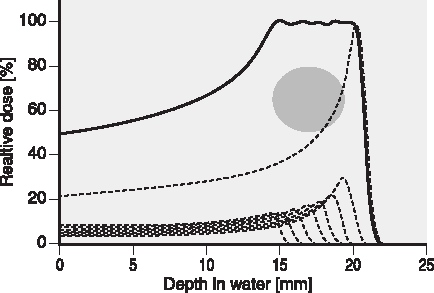
\includegraphics[width=\textwidth, scale=0.50]{sobp.pdf}
			\caption{Creazione di SOBP per un fascio singolo di protoni. La curva spessa rappresenta la dose rilasciata nel target (individuato dal cerchio grigio), ottenuta dalla somma dei singoli BP a differenti energie (indicati con una linea tratteggiata) \cite{Bomford2002-wo}.}
			\label{fig:sobp}
		\end{subfigure}
		\par
		\begin{subfigure}[t]{0.49\textwidth}
			\centering
			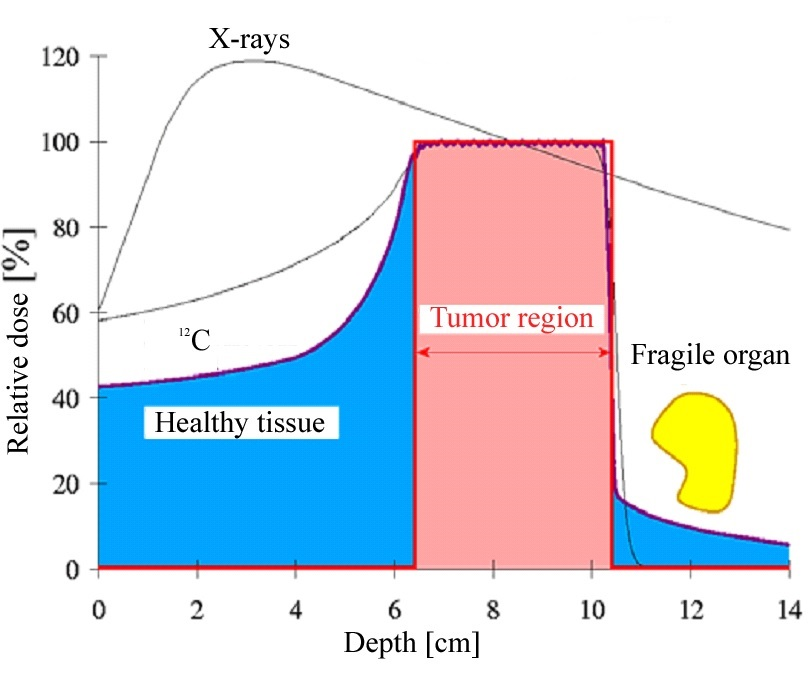
\includegraphics[width=\textwidth, scale=0.50]{critical_organ.jpg}
			\caption{Profili di dose di raggi X, protoni e atomi di carbonio in funzione della profondità. La presenza del BP consente di risparmiare l'organo a rischio, colpito invece dal fascio di raggi X \cite{unipv_conference2}.}
			\label{fig:critical_organ}
		\end{subfigure}
		\caption{Proprietà e applicazioni del picco di Bragg.}
	\end{figure}
	Tornando alla \hyperref[fig:photon]{Fig. 1.17}, è evidente che il rilascio energetico del fascio di atomi di carbonio \ce{C}, a differenza del caso dei protoni \ce{p}, prosegue anche dopo il BP.\footnote{Un rilascio energetico dopo il BP potrebbe ledere regioni sane situate dopo il volume tumorale, pertanto è necessario comprendere la sua cagione.} Osservando l'andamento quadratico $\propto\frac{z^2}{\beta^2}$ della \hyperref[eq:bethe_bloch]{Eq. 1.35}, pur essendo $z_p<z_C$, si ha che $\frac{dE_p}{dx}>\frac{dE_C}{dx}$ in quanto le energie cinetiche dei carboni sono maggiori di quelle dei protoni.\footnote{Solitamente le energie cinetiche $K$ sono $K_p=250 \mbox{ MeV}$ e $K_C=4800\mbox{ MeV}=12\mbox{ u}\cdot400\mbox{ MeV/u}$.} In effetti, il profilo di dose rilasciato dai fasci di carbonio è generalmente maggiore di quello dei protoni: ciò spiegherebbe i maggiori valori di \hyperref[par:let]{LET} e \hyperref[par:rbe]{RBE} per il carbonio della \hyperref[tab:let_rbe]{Tab. 1.2}, ma non il rilascio di energia dopo il BP da parte del carbonio. \'E possibile comprendere tale effetto solo analizzando le interazioni nucleari delle due particelle.
	
	\subsubsection{Interazioni nucleari}\label{par:interazioni_nucleari}
	Pur essendo le interazioni elettromagnetiche più frequenti di quelle nucleari, gli effetti di queste ultime risultano fondamentali nelle applicazioni adroterapiche. Per interagire con i nuclei della materia, le particelle cariche devono possedere un'energia sufficientemente elevata da consentire un superamento della barriera di potenziale coulombiana dovuta alle cariche di elettroni e protoni, per fare in modo che i nuclei del proiettile e del bersaglio siano molto vicini tra di loro. Infatti, le forze nucleari (la forza forte che lega i nucleoni\footnote{Protoni e neutroni.} all'interno del nucleo atomico), a differenza della forza elettromagnetica, possiedono una natura a corto raggio d'azione dell'ordine del raggio dei nucleoni, pari a $\approx1\mbox{ fm}$. Tra i vari effetti delle interazioni nucleari si possono citare il grazing (in cui il nucleo proiettile effettua un ``passaggio radente'' al nucleo bersaglio generando, ad esempio, il trasferimento di più nucleoni), le collisioni anelastiche (dove vi è una grande dissipazione di energia e i nuclei possono restare sostanzialmente intatti o trasformarsi radicalmente) e le fusioni nucleari (in cui si genera un nucleo composto che decade dopo $10^{-18}$--$10^{-19}\mbox{ s}$ o emettendo raggi $\gamma$, protoni, neutroni, particelle $\alpha$ o, per fissione, in frammenti più piccoli) \cite{treccani_ioni_pesanti}. Nei range energetici utilizzati in adroterapia ($\approx100\mbox{ MeV/u}$) l'interazione nucleare più comune è la frammentazione.
	
	La frammentazione nucleare si suddivide in collisioni periferiche e centrali. Le prime, essendo caratterizzate da bassi scambi di energia e quantità di moto (che avvengono tra i cosiddetti nuclei partecipanti), sono caratterizzate da una bassa molteplicità\footnote{In altre parole generano poche particelle e frammenti del target secondari.}; durante tali eventi si hanno anche nuclei spettatori (sia del proiettile che del target) che si disintegrano mediante processi di frammentazione o evaporazione. Nelle collisioni centrali (a queste energie meno frequenti delle precedenti) si ha una grande molteplicità di particelle e frammenti generati e vi sono solo nuclei partecipanti \cite{lnf_document}. La \hyperref[fig:fragmentation]{Fig. 1.36} illustra la dinamica più frequente delle collisioni periferiche che, secondo il modello di Serber \cite{PhysRev.72.1114}, è suddivisa in una fase di abrasione (in cui i nuclei coinvolti interagiscono formando frammenti e uno stato eccitato denominato fireball nucleare), che avviene in tempi di $10^{-22}$--$10^{-23}\mbox{ s}$, e in una di ablazione (dove processi di termalizzazione diseccitano la fireball e producono frammenti secondari sia del proiettile che del bersaglio), che avviene in tempi di $10^{-16}$--$10^{-18}\mbox{ s}$.
	\begin{figure}[H]
		\centering
		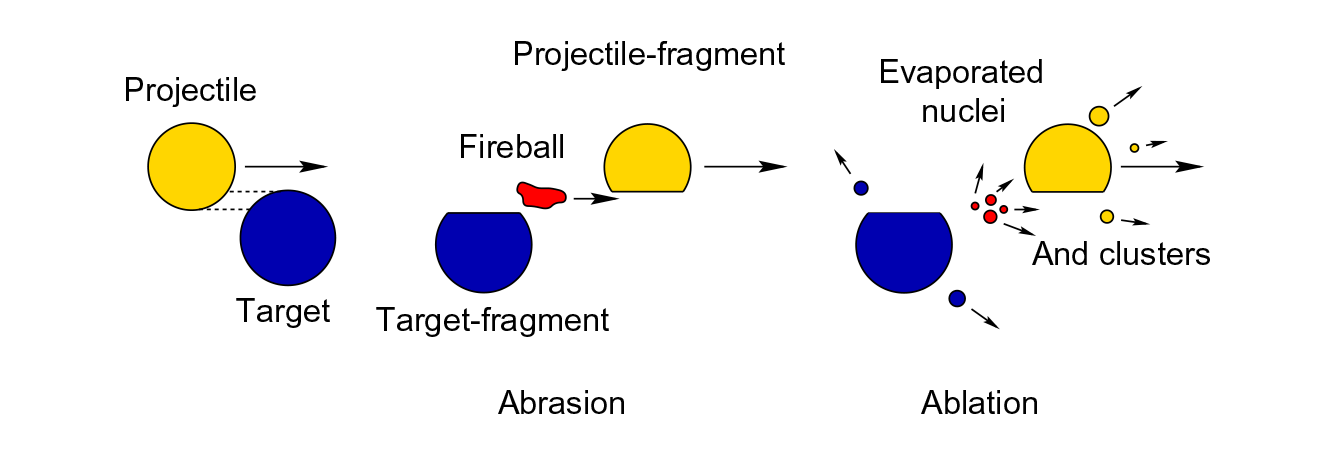
\includegraphics[width=0.9\linewidth]{fragmentation.png}
		\caption{Schema dei processi di abrasione e ablazione (per evaporazione) nel modello di interazione periferica della frammentazione di Serber \cite{Schardt2010-bc}.}
		\label{fig:fragmentation}
	\end{figure}
	Come già accennato, quando particelle proiettile come protoni o ioni pesanti come ioni carbonio colpiscono il corpo umano, si può generare una frammentazione sia del proiettile che del target. Sebbene entrambi i processi siano caratterizzati dall'emissione di frammenti leggeri, a seguito del primo si produce anche un quasi-proiettile dotato di un'energia (circa) pari a quella del proiettile incidente, mentre dopo il secondo si genera un quasi-target (circa) a riposo. Considerando che nei range energetici adroterapici non è possibile frammentare il protone in quark (i suoi costituenti elementari),\footnote{Per farlo è necessaria un'energia $\approx\mbox{GeV}$.}, le possibilità di frammentazione di un proiettile che interagisce con un target a riposo sono riassunte nella \hyperref[tab:fragmentation]{Tab. 1.4}.
	\begin{table}[H]
		\begin{minipage}{\textwidth}
			\centering
			\begin{tabular}{ |M{2.87cm}|M{2.87cm}||m{7.7cm}| }
				\hline
				Proiettile & Target & Processo\\
				\hline\hline
				Protone & Protone & Non avviene frammentazione\\
				\hline
				Protone & Ione pesante & Frammentazione del target\\
				\hline
				Ione pesante & Protone & Frammentazione del proiettile\\
				\hline
				Ione pesante & Ione pesante & Frammentazione del target e del proiettile\\
				\hline
			\end{tabular}
		\end{minipage}
		\caption{Tabella riassuntiva della frammentazione del target e del proiettile. In adroterapia solitamente si considera un proiettile di energia $\approx200\mbox{ MeV/u}$ e il target a riposo.}
		\label{tab:fragmentation}
	\end{table}
	Da un punto di vista pratico è molto complesso studiare i frammenti del target in quanto possiedono un range molto piccolo che va dai $2.3\mbox{ }\mu\mbox{m}$ di \ce{^{15}O} al $68.9\mbox{ }\mu\mbox{m}$ di \ce{^{2}H} (si veda \hyperref[tab:range]{Tab. 2.1}); in sostanza, è come se i frammenti del target venissero prodotti a riposo. Pertanto, le proprietà dei frammenti del target non possono essere misurate tramite tecniche di rivelazione convenzionale ma sono necessari approcci differenti come quello della \hyperref[sec:cinematica_inversa]{cinematica inversa}, utilizzato nell'esperimento FOOT. D'altra parte, misurare le proprietà dei frammenti del proiettile è più semplice in quanto il loro elevato range consente di applicare metodi di rivelazione convenzionali.
	\begin{figure}[H]
		\centering
		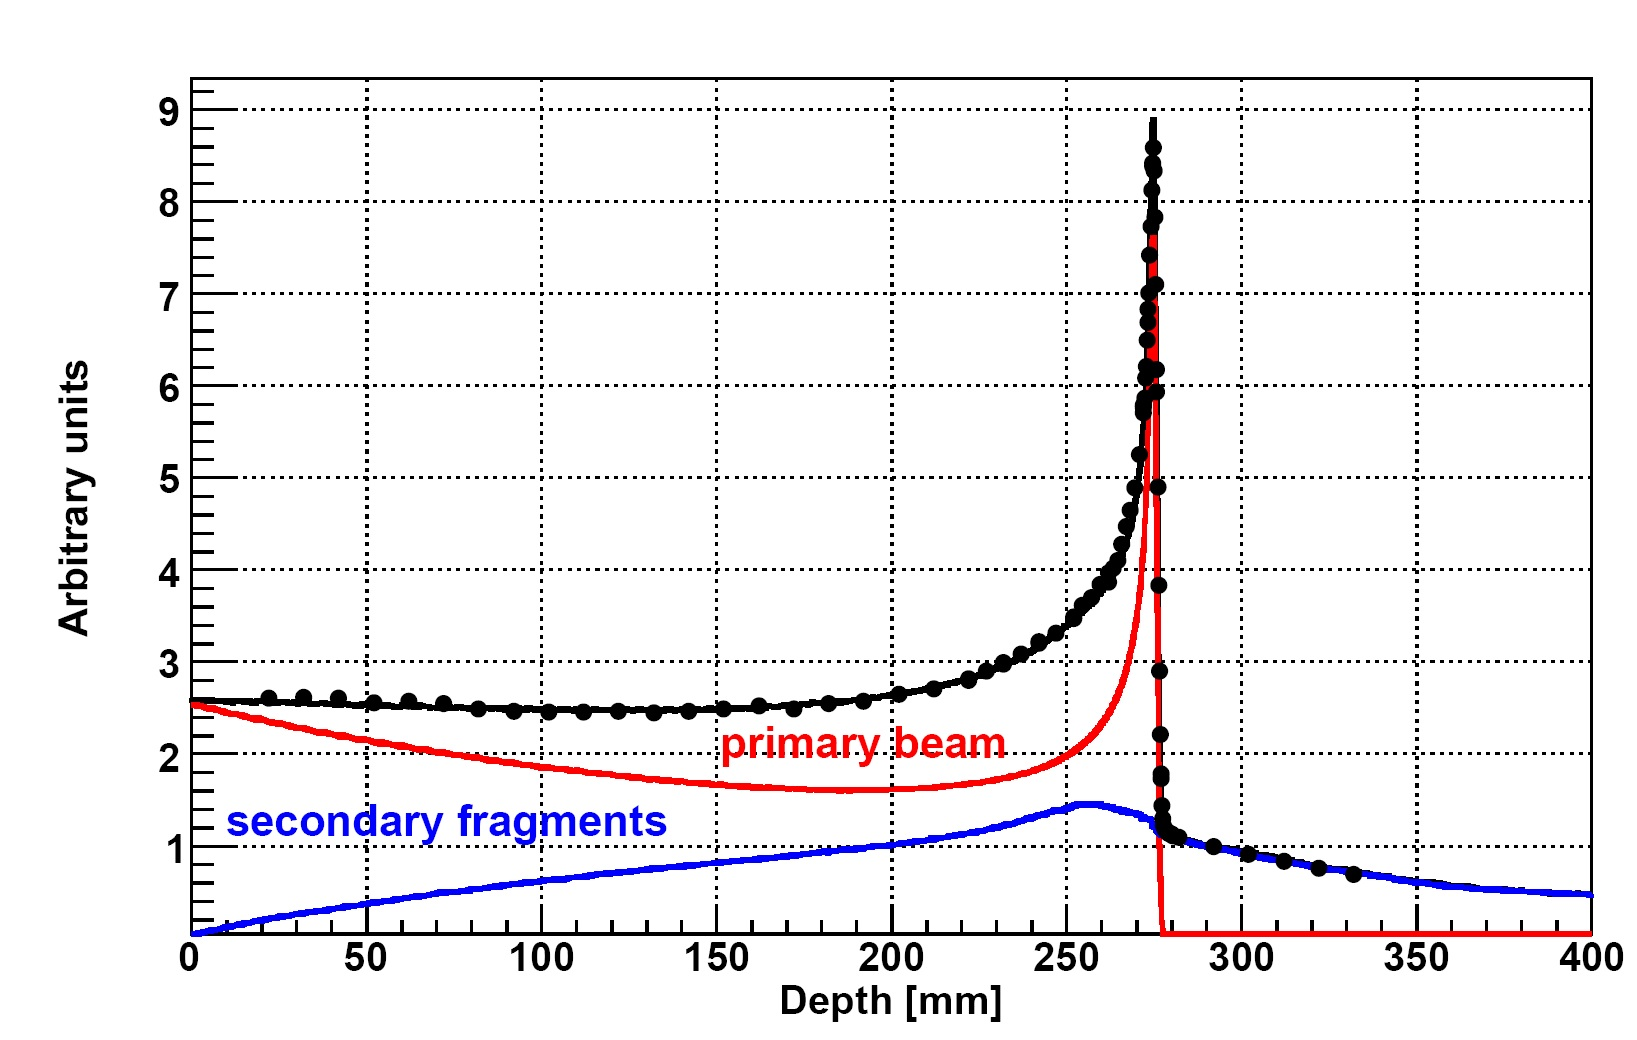
\includegraphics[width=0.78\linewidth]{late_release.jpg}
		\caption{Dati sperimentali della dose totale in funzione della profondità per un fascio di \ce{C} a $400\mbox{ MeV/u}$ in acqua. La diminuzione di energia del fascio primario (curva rossa) nel canale di ingresso è dovuta alla frammentazione che genera frammenti secondari (curva blu) il cui contributo è particolarmente evidente dopo il BP. I due contributi si sommano fornendo la dose totale (curva nera) \cite{mairani}.}
		\label{fig:late_release}
	\end{figure}
	Riprendendo la \hyperref[fig:photon]{Fig. 1.17}, ora è possibile comprendere il motivo per cui si verifica un rilascio di dose dopo il BP per particelle cariche pesanti. Tale contributo è dovuto al lungo range dei frammenti del proiettile che, avendo un numero atomico $z$ inferiore al fascio incidente primario\footnote{Poiché i frammenti si originano dalla fissione del nucleo primario.} e circa lo stesso $\beta$, per la \hyperref[eq:bethe_bloch]{Eq. 1.35} possiedono un minore potere frenante;\footnote{Secondo tale considerazione, per penetrare più in profondità basterebbe scegliere fasci formati da particelle con qualsiasi valore di $z$, purché sia elevato; in pratica, ciò non è possibile in quanto i processi di frammentazione sarebbero così elevati da rilasciare energie troppo alte nel canale di ingresso, dove si vuole avere un basso dosaggio per risparmiare i tessuti sani. Pertanto, ioni più pesanti dell'ossigeno non vengono ritenuti efficaci in adroterapia.} perdendo meno energia per unità di lunghezza, i frammenti del proiettile dissipano la loro energia più in profondità rispetto alle particelle proiettile primarie (queste ultime, infatti, si bloccano generalmente in corrispondenza del picco di Bragg,\footnote{In realtà la sopravvivenza di proiettili primari è fortemente legata alla loro energia e al loro numero atomico (più è grande e più interazioni compiono durante il percorso, essendo la \hyperref[eq:bethe_bloch]{Eq. 1.35} $\propto z^2$). Ad esempio, un fascio di \ce{^{12}C} a $400\mbox{ MeV}$ ha un range di $28\mbox{ cm}$. A tale profondità il $70\%$ dei \ce{^{12}C} ha già effettuato processi di frammentazione del proiettile prima di giungere al BP; nonostante ciò, nel BP si verifica comunque un grande rilascio di dose in quanto vi contribuiscono non solo le poche particelle primarie rimanenti, ma anche quelle secondarie (che nella maggior parte dei casi sono isotopi, isotoni o isobari delle primarie).} come mostrato in \hyperref[fig:late_release]{Fig. 1.37}).
	\begin{figure}[H]
		\centering
		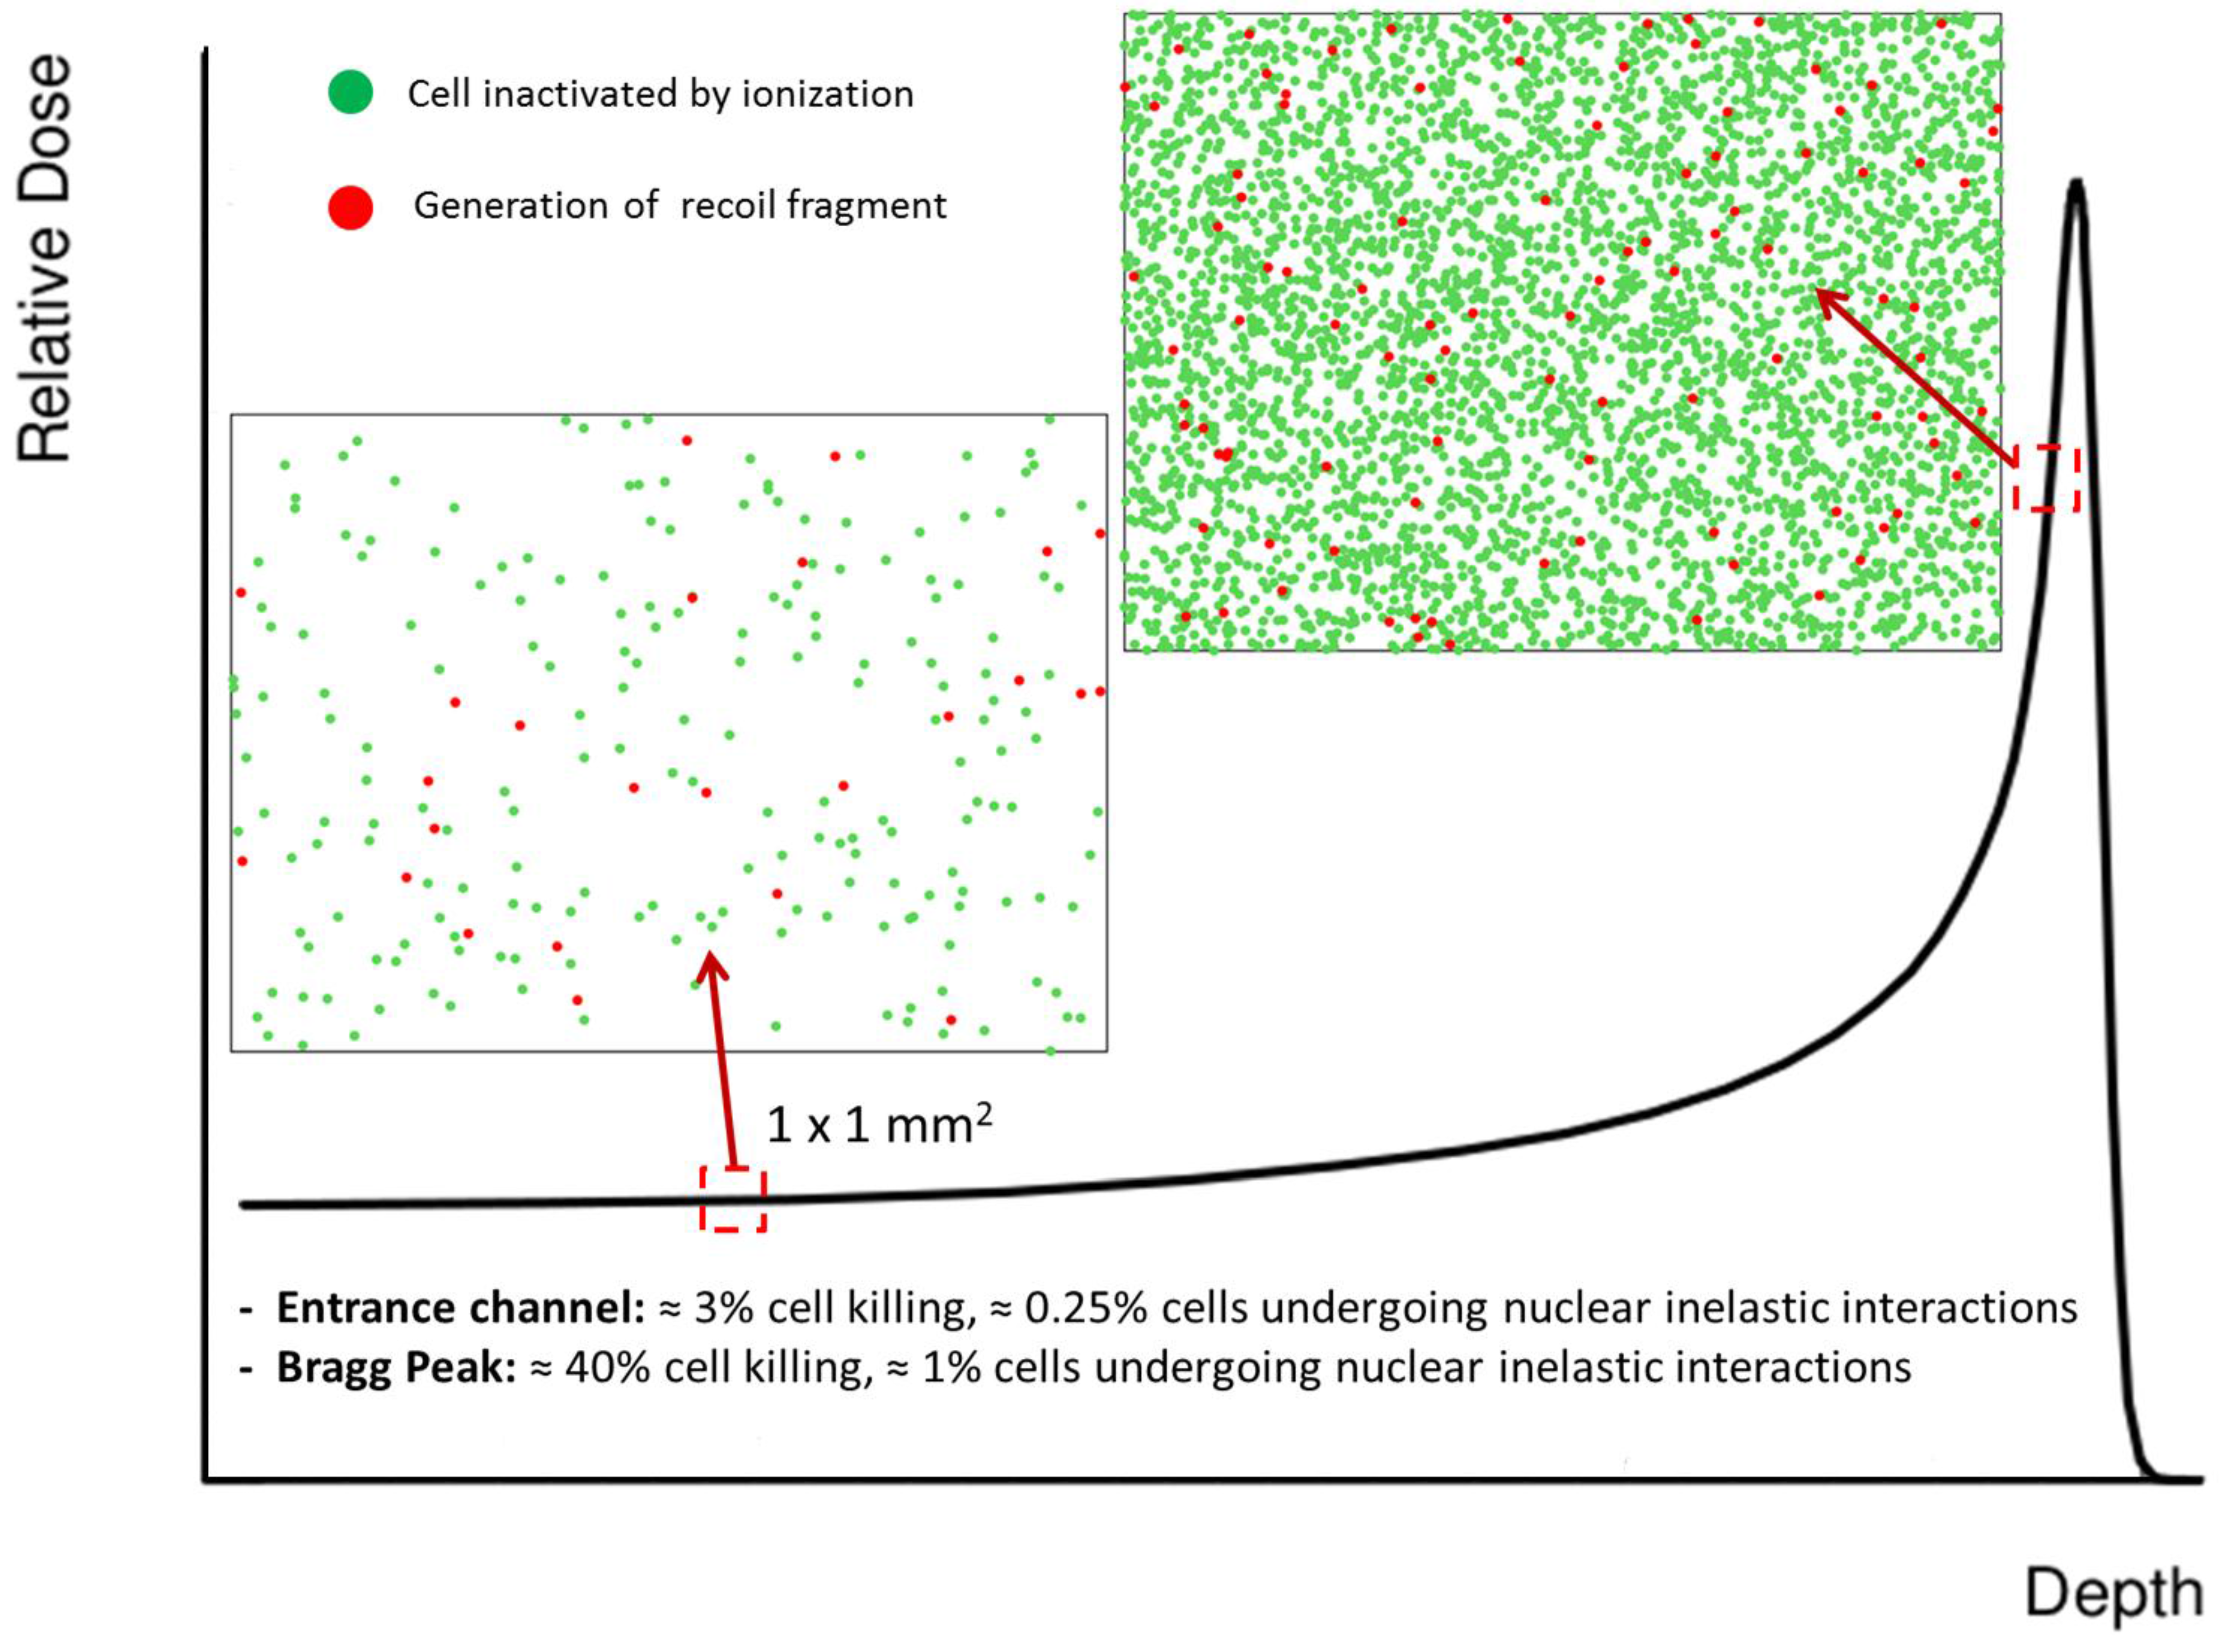
\includegraphics[width=0.82\linewidth]{biol_effect_nuclear.png}
		\caption{Impatto dei frammenti del target per un fascio protonico a $250\mbox{ MeV}$ in acqua nel canale di ingresso e nella regione di picco e relativa ionizzazione \cite{cancers7010353}.}
		\label{fig:biol_effect_nuclear}
	\end{figure}
	Dalla \hyperref[fig:biol_effect_nuclear]{Fig. 1.38} è possibile valutare l'effetto delle interazioni nucleari sulle cellule. In particolare, si osserva che la frammentazione del target per un fascio di protoni è molto più rilevante nel canale di ingresso che nella regione del picco di Bragg, sebbene l'effetto della ionizzazione nelle due zone sia molto differente. Infatti, la ionizzazione uccide rispettivamente il $3\%$ e il $40\%$ delle cellule nel canale di ingresso e nel BP ma l'interazione nucleare è responsabile rispettivamente solo dell'$8\%$ e del $2\%$ delle morti cellulari totali.
	
	A differenza delle interazioni elettromagnetiche, i processi di frammentazione nucleare non sono solamente più difficili da modellizzare con le teorie di cui disponiamo attualmente, ma anche più complessi da misurare sperimentalmente. Per usufruire delle peculiarità delle particelle cariche (una tra tutte il picco di Bragg), sfruttandole ad esempio nell'ottimizzazione del trattamento clinico dei tumori, è necessario giungere a una completa conoscenza dei processi di interazione delle particelle con il corpo umano, in particolare dei processi di frammentazione nucleare, al momento non compresi del tutto. Esistono modelli semiempirici (come la legge di Bradt-Peters) che consentono di ricavare, con ottimi risultati, le sezioni d'urto di alcune interazioni nucleari, conoscendo la struttura dei nuclei del target e del proiettile, ma ciò non è abbastanza: bisognerebbe includere nei modelli la totalità dei contributi forniti dai frammenti nucleari, la cui numerosità è elevatissima. Come verrà esposto nel \hyperref[cap:2]{Cap. 2}, l'obiettivo principale dell'esperimento FOOT è proprio quello di arricchire la quantità di dati attualmente a disposizione misurando la sezione d'urto, l'energia e la direzione di produzione dei frammenti secondari generati a partire dalle interazioni nucleari tra particelle cariche e corpo umano, in modo da migliorare la descrizione di parametri dosimetrici fondamentali nel TP, come l'RBE. In particolare, oltre ai fasci di protoni e atomi di carbonio, FOOT intende misurare con più precisione i frammenti nucleari dei fasci di ossigeno ed elio, visto che il loro uso in adroterapia è ancora in fase di sperimentazione.
	
	\chapter{Esperimento FOOT}\label{cap:2}
	I processi di frammentazione nucleare tipici dei range energetici delle applicazioni adroterapiche ($50$--$250\mbox{ MeV}$ per i protoni e $50$--$400\mbox{ MeV/u}$ per gli ioni carbonio) presentano evidenti lacune sperimentali. Ciò ha obbligato gli scienziati a sviluppare modelli di frammentazione basati su simulazioni che, in assenza di una precisa teoria dei frammenti nucleari, sono caratterizzate da numerose incertezze. Recentemente, in alcuni esperimenti, si è misurata la frammentazione del proiettile degli ioni di \ce{^{12}C}, tuttavia tali misure coprono solo la parte inferiore dei range energetici sopra citati \cite{PhysRevC.88.024606,PhysRevC.93.064601}. Inoltre, esistono alcune misure riguardanti i processi di frammentazione del target, che però si limitano alla produzione di frammenti molto leggeri ($Z<3$) e sono caratterizzate da una bassa accuratezza, dovuta soprattutto al corto raggio ($\approx\mu\mbox{m}$) dei frammenti del target che non consente di misurare le loro proprietà con tecniche di rivelazione convenzionali. Tali problematiche hanno portato a un progressivo abbandono degli studi afferenti alla frammentazione del target, specialmente quella indotta da fasci protonici; sempre per tali motivi, vi è una grande scarsità di dati anche per i frammenti generati da bersagli più pesanti, dotati di maggiori $A$ e $Z$ \cite{foot_cdr}.
	
	Per supplire a tali mancanze, sia della frammentazione del target che del proiettile, è nato l'esperimento FOOT (FragmentatiOn Of Target), il cui scopo principale è quello di misurare (con un'incertezza massima del $5\%$) le sezioni d'urto dei processi di frammentazione nucleare nel range energetico $100$--$800\mbox{ MeV/u}$, che coinvolgono frammenti caratterizzati da $2<Z<10$ \cite{ubaldiArticle}. Oltre a misurare la frammentazione del target indotta da fasci protonici con l'ausilio della \hyperref[sec:cinematica_inversa]{cinematica inversa}, FOOT si impegna a completare le misure di frammentazione del proiettile generate da fasci di \ce{C}, \ce{O}\footnote{I fasci di \ce{O} risultano particolarmente efficaci contro tumori ipossici (per i motivi esposti in \hyperref[par:oer]{OER} \cite{Tommasino2016-qb}), sebbene in condizioni aerobiche producano più danni nel canale di ingresso (a causa del loro elevato $Z$) comparati a ioni più leggeri come i \ce{C}.} ed \ce{He}\footnote{I fasci di \ce{He} possiedono un rilascio di dose più preciso rispetto a quello dei protoni (essendo i primi caratterizzati da meno eventi di \hyperref[par:scattering_Rutherford]{scattering Rutherford} (rispetto ai protoni) e di \hyperref[par:interazioni_nucleari]{frammentazione nucleare} (rispetto ai \ce{C}) \cite{Grun2015-ln,articleIndelicato}. Inoltre, rispetto agli altri ioni ad alto LET come i \ce{C}, l'uso di \ce{He} prevede costi più contenuti.} tramite la cinematica diretta.
		
	Misure più accurate degli spettri energetici e delle sezioni d'urto dei frammenti nucleari risulterebbero di fondamentale importanza per la progettazione di nuovi sistemi di TP adroterapici, come i BioTPS, in cui avviene una valutazione minuziosa\footnote{Esistono algoritmi \cite{steinstrater2015integration} che consentono di ottenere una proiezione voxel-by-voxel del profilo di dose efficace (pesata attraverso l'RBE) prima del rilascio in una regione tissutale.} di tutti i possibili effetti biologici indotti dal fascio radiativo, inclusi i contributi dovuti ai frammenti nucleari (che sono molto complicati da valutare, in quanto dipendenti dai differenti tipi di particelle in gioco e dalle loro singole energie).
	
	I risultati di FOOT saranno utili anche per applicazioni legate alla radioprotezione spaziale, un tema che desta interesse ad agenzie spaziali come la NASA che, da alcuni anni, svolge programmi di ricerca in cui si valutano i rischi radiativi a cui si potrebbero sottoporre gli astronauti nelle missioni spaziali di lunga durata (come in eventuali viaggi su Marte) \cite{RevModPhys.83.1245}. Infatti, al di fuori dell'atmosfera terrestre, vi è una grande quantità di radiazione (cosmica, come la GCR\footnote{Galactic Cosmic Radiation.} o provocata da brillamenti solari, come le SPE\footnote{Solar Particle Events.} \cite{ridolfiArticle}) che rappresenta un vero rischio non solo per l'equipaggio ma anche per tutta la componentistica elettronica presente in orbita \cite{foot_site}. Pertanto, una dettagliata conoscenza dei processi di frammentazione nucleare si rivelerebbe utile anche ai programmi di radioprotezione spaziale, per esempio attraverso la progettazione di materiali radioresistenti in grado di schermare gli effetti nocivi della radiazione cosmica che migliorerebbero gli attuali sistemi di protezione delle navicelle spaziali \cite{foot_cdr}.
	
	\section{Cinematica inversa}\label{sec:cinematica_inversa}
	Come già più volte discusso, la rivelazione dei frammenti del target risulta piuttosto complicata per il loro corto raggio (si veda \hyperref[tab:range]{Tab. 2.1}) e per la loro bassa energia (di pochi $\mbox{MeV}$) \cite{foot_cdr}. Per superare tali difficoltà, si potrebbe pensare all'impiego di targhette sottili con le quali sarebbe possibile un'eventuale espulsione (e una conseguente rivelazione) dei frammenti, ma ciò risulterebbe ulteriormente problematico; infatti, una targhetta sottile causerebbe un abbassamento della probabilità di interazione fascio-materia,\footnote{Si pensi che la probabilità di avere eventi di frammentazione nucleare è già molto bassa poiché si attesta attorno a $10^{-2}$.} che porterebbe a prese dati troppo lunghe (e costose). Inoltre, anche se si utilizzasse una targhetta sottile, sarebbe possibile misurare solo l'energia posseduta dai frammenti al termine dell'attraversamento target e non la loro energia di produzione (che è la grandezza che si vuole conoscere). Per ovviare a tali difficoltà, FOOT utilizza una tecnica già adottata in altri esperimenti \cite{PhysRevC.88.024606,webber1990individual,10.3389/fphy.2022.979229} chiamata cinematica inversa.
	\begin{table}[H]
		\begin{minipage}{\textwidth}
			\centering
			\begin{tabular}{ |M{3.28cm}|M{3.28cm}|M{3.28cm}|M{3.28cm}| }
				\hline
				Frammento & E $\left[\mbox{MeV}\right]$&LET $\left[\mbox{keV/}\mu\mbox{m}\right]$&Range $\left[\mu\mbox{m}\right]$\\
				\hline\hline
				\ce{^{15}O}&1.0&983&2.3\\
				\hline
				\ce{^{15}N}&1.0&925&2.5\\
				\hline
				\ce{^{14}N}&2.0&1137&3.6\\
				\hline
				\ce{^{13}C}&3.0&951&5.4\\
				\hline
				\ce{^{12}C}&3.8&912&6.2\\
				\hline
				\ce{^{11}C}&4.6&878&7.0\\
				\hline
				\ce{^{10}B}&5.4&643&9.9\\
				\hline
				\ce{^{8}Be}&6.4&400&15.7\\
				\hline
				\ce{^{6}Li}&6.8&215&26.7\\
				\hline
				\ce{^{4}He}&6.0&77&48.5\\
				\hline
				\ce{^{3}He}&4.7&89&38.8\\
				\hline
				\ce{^{2}H}&2.5&14&68.9\\
				\hline
			\end{tabular}
		\end{minipage}
		\caption{Parametri fisici dei frammenti del target prodotti in acqua da un fascio protonico di $180\mbox{ MeV}$. L'energia iniziale media dei frammenti viene valutata con la formula semiempirica di Goldhaber \cite{cancers7010353,GOLDHABER1974306}.}
		\label{tab:range}
	\end{table}
	Se nella cinematica diretta un processo di frammentazione del target\footnote{Il target solitamente si compone di atomi di \ce{H}, \ce{O} e \ce{C}, poiché i tessuti del corpo umano sono costituiti dal $65\%$ di \ce{H}, dal $24\%$ di \ce{O} e dal $10\%$ di \ce{C}.} indotto da un fascio di protoni (per esempio di energia $200\mbox{ MeV}$) viene osservato nel sistema di riferimento in cui il target è a riposo, nella cinematica inversa avviene il procedimento inverso: un bersaglio di protoni (solitamente costituito da \ce{H}) a riposo viene irradiato da un fascio di \ce{C} o \ce{O} (di energia $200\mbox{ MeV/u}$), elementi che costituivano il target della cinematica diretta,\footnote{Per questo la cinematica inversa protonica consente anche di ottenere misure della frammentazione del proiettile prodotte dalla cinematica diretta dei fasci di \ce{C} e \ce{O}.} i cui frammenti nucleari sono dotati di un lungo raggio che consente una rivelazione più agevole. Chiaramente, per ottenere le misure di quantità di moto ed energia nel sistema di riferimento originario (in cui i nuclei di \ce{C} e \ce{O} si trovano a riposo), si devono applicare le trasformazioni (boost) di Lorentz, operazioni che (per ridurre la propagazione di incertezze) richiedono non solo un grande livello di accuratezza nelle misure di energia e momento sia dei frammenti prodotti sia delle particelle del fascio, ma anche una risoluzione angolare dell'angolo di emissione (rispetto alla direzione entrante del fascio) di particelle incidenti e frammenti dell'ordine dei $\mbox{mrad}$, che impone uno spessore del target massimo di pochi $\mbox{mm}$ \cite{foot_cdr}.
	
	Dato che l'\ce{H} è altamente infiammabile, la realizzazione di targhette di \ce{H} puro necessiterebbe di sistemi di raffreddamento avanzati e condizioni di vuoto spinto.\footnote{Poiché l'idrogeno si trova allo stato gassoso a temperatura ambiente.} Pertanto, per riprodurre un bersaglio di \ce{H}, si utilizzano separatamente due target di \ce{C} e polietilene (\ce{C2H4}). Quindi, la sezione d'urto su \ce{H} si ottiene per sottrazione delle sezioni d'urto su \ce{C} e \ce{C2H4}:
	\begin{equation}
		\left(\frac{d\sigma}{dE_k}\right)_{H}=\frac{1}{4}\left[\left(\frac{d\sigma}{dE_k}\right)_{{C_2H_4}}-2\left(\frac{d\sigma}{dE_k}\right)_{{C}}\right]
		\label{eq:c2h4}
	\end{equation}
	dove $\left(\frac{d\sigma}{dE_k}\right)_{H}$, $\left(\frac{d\sigma}{dE_k}\right)_{{C_2H_4}}$ e $\left(\frac{d\sigma}{dE_k}\right)_{{C}}$ sono le sezioni d'urto differenziali rispetto all'energia cinetica $E$ di un particolare frammento prodotto $k$.
		
	\section{Apparato sperimentale}\label{sec:apparato_sperimentale}
	La progettazione dell'apparato sperimentale di FOOT è avvenuta seguendo specifiche richieste strutturali differenti. In primo luogo, si richiedevano dimensioni contenute per garantire la sua portabilità in centri adroterapici\footnote{Attualmente l'apparato sperimentale di FOOT si trova al \hyperref[sec:adroterapia_italia]{CNAO} a Pavia.} dotati di fasci terapici differenti. Inoltre, dato che l'approccio cinematico inverso impone un'elevata accuratezza delle misure sperimentali, l'apparato di FOOT presenta delle ``ridondanze'', con le quali è possibile risalire a una medesima grandezza fisica attraverso modalità differenti; per esempio, ciò avviene nell'identificazione del numero di massa dei frammenti (si vedano le \hyperref[eq:a1]{Eq. 2.3a}, \hyperref[eq:a2]{Eq. 2.3b} ed \hyperref[eq:a3]{Eq. 2.3c}).
	
	Simulazioni Montecarlo basate sul codice FLUKA \cite{Ferrari:2005zk,BOHLEN2014211}, confermate dai dati sperimentali, hanno predetto che i frammenti più pesanti ($Z>2$) vengono emessi entro un angolo rispetto alla direzione del fascio piuttosto ridotto ($\approx10^\circ$) e con una distribuzione di energia cinetica per nucleone piccata in corrispondenza dell'energia cinetica del fascio primario entrante; al contrario, i frammenti più leggeri ($Z\le2$) vengono prodotti con distribuzioni angolari molto più ampie (come mostrato in \hyperref[fig:angular]{Fig. 2.1}) ed energie cinetiche dotate di maggiore variabilità. Per tali motivi l'apparato sperimentale di FOOT è suddiviso in due setup sostanzialmente complementari:
	\begin{itemize}
		\item elettronico (per frammenti pesanti): dotato di un'accettanza angolare di $\pm10^\circ$ rispetto alla direzione del fascio, è costituito da detector elettronici e da uno spettrometro magnetico. \'E in grado di identificare e misurare frammenti più pesanti di \ce{^{4}He}.
		\item Camera a emulsione (per frammenti leggeri): dotato di un'accettanza angolare maggiore di $50^\circ$ rispetto alla direzione del fascio, è dotato di una camera a emulsione con la quale poter misurare frammenti leggeri come protoni, deuteroni (nuclei del deuterio), tritoni (nuclei del trizio) e nuclei di \ce{He}.
	\end{itemize}
	\begin{figure}[H]
		\centering
		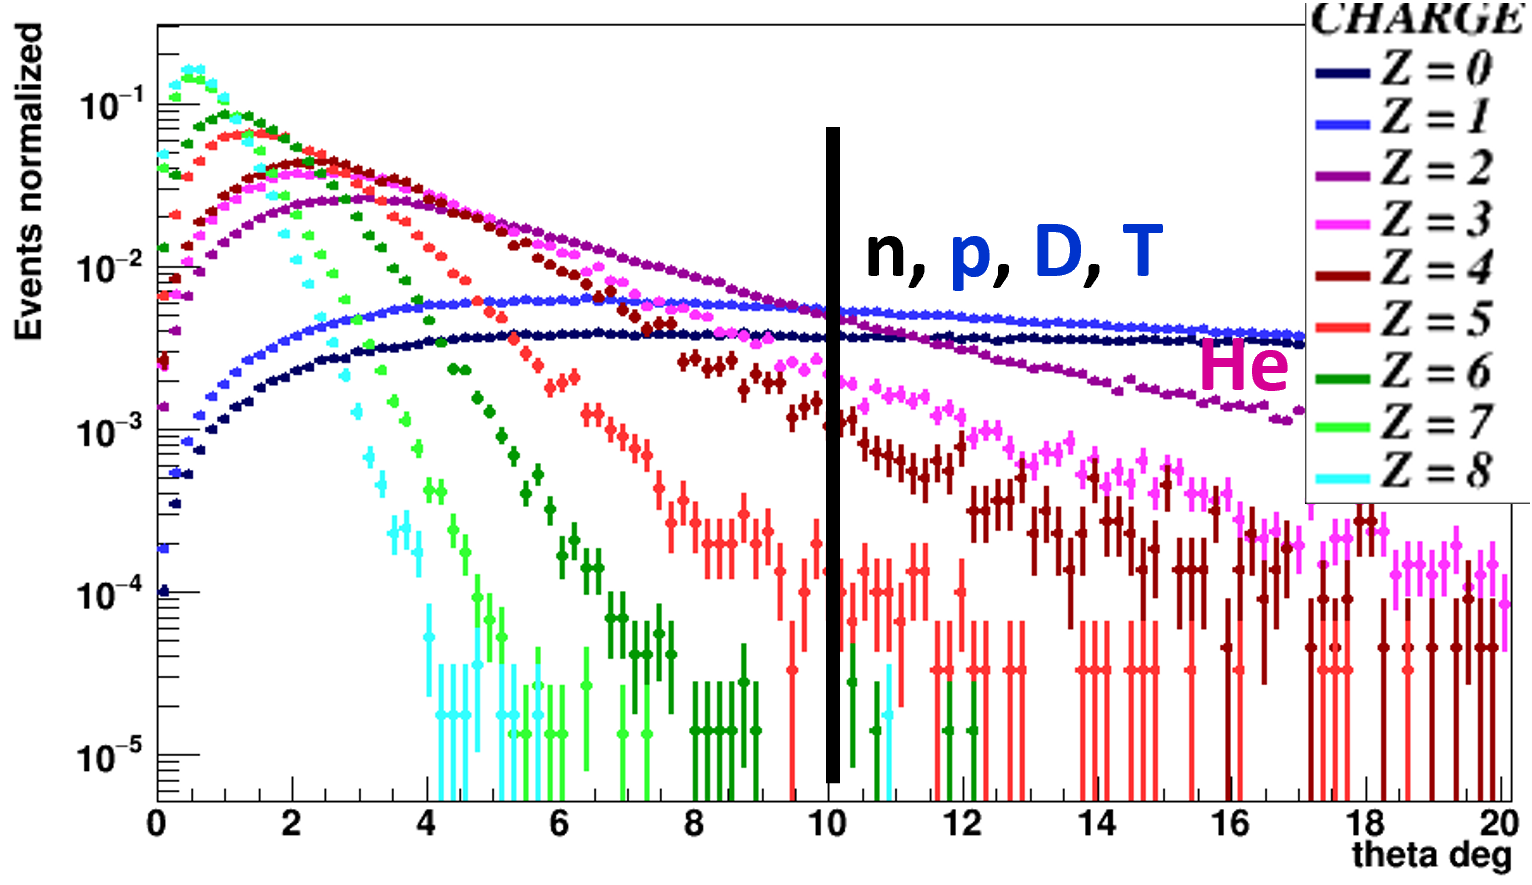
\includegraphics[width=0.8\linewidth]{angular.png}
		\caption{Angolo di emissione $\theta$ dei frammenti in una serie di eventi normalizzati. A valori maggiori di $\theta$ sono legati frammenti con un numero atomico $Z$ più elevato \cite{slide_spighi}.}
		\label{fig:angular}
	\end{figure}
	
	\subsection{Setup elettronico}\label{sec:setupElettronico}
	\begin{figure}[H]
		\centering
		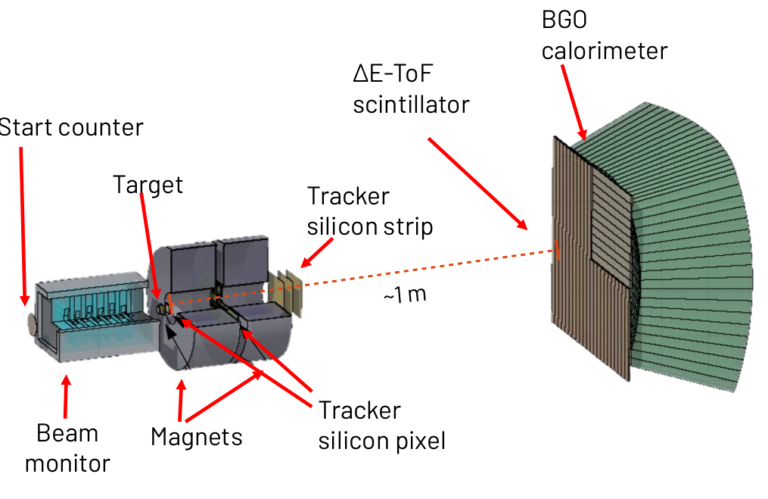
\includegraphics[width=0.9\linewidth]{electronic_setup.png}
		\caption{Schematizzazione del setup elettronico utilizzato in FOOT \cite{foot_site2}.}
		\label{fig:electronic_setup}
	\end{figure}
	Il setup elettronico di FOOT è costituito da vari sub-detector (si veda \hyperref[fig:electronic_setup]{Fig. 2.2}) con i quali è possibile attuare la ricostruzione isotopica dei frammenti prodotti e l'individuazione della loro carica. Ciò avviene tramite la misura di quantità di moto, energia cinetica e tempo di volo (Time Of Flight, TOF) dei frammenti nucleari \cite{foot_cdr}. Il rilascio di energia dei frammenti per unità di distanza percorsa $\frac{dE}{dx}$ viene misurato più volte analizzando l'energia depositata $\Delta E$ dai frammenti all'interno dell'apparato di misura. La carica delle particelle viene identificata combinando le misure di $\Delta E$ con quelle del TOF, mentre la massa a riposo $m$ dei frammenti\footnote{Quindi anche il loro numero di massa $A$.} viene estratta dalle misure di momento $p$, energia cinetica $E_k$ e TOF attraverso le seguenti relazioni relativistiche:
	\begin{subequations}
		\begin{align}
			\label{eq:momentum}
			p&=mc\beta\gamma\\
			\label{eq:kinetic_energy1}
			E_k&=mc^2\left(\gamma-1\right)\\
			\label{eq:kinetic_energy2}
			E_k&=\sqrt{p^2c^2+m^2c^4}-mc^2
		\end{align}
	\end{subequations}
	dove $\beta$ è la velocità del frammento in unità di $c$ (velocità della luce nel vuoto) e $\gamma=\frac{1}{\sqrt{1-\beta^2}}$ è il fattore di Lorentz. Dalle \hyperref[eq:momentum]{Eq. 2.2a}, \hyperref[eq:kinetic_energy1]{Eq. 2.2b} ed \hyperref[eq:kinetic_energy2]{Eq. 2.2c} è possibile determinare il numero di massa $A$ in tre modi differenti:
	\begin{subequations}
		\begin{align}
			\label{eq:a1}
			A_1&=\frac{p}{u\beta c\gamma}\\
			\label{eq:a2}
			A_2&=\frac{E_k}{uc^2\left(\gamma-1\right)}\\
			\label{eq:a3}
			A_3&=\frac{p^2c^2-E_k^2}{2uc^2E_k}
		\end{align}
	\end{subequations}
	dove $u$ è l'unità di massa atomica ($\approx931.5\mbox{ MeV}$). Come si evincerà nel prosieguo, le \hyperref[eq:a1]{Eq. 2.3a}, \hyperref[eq:a2]{Eq. 2.3b} ed \hyperref[eq:a3]{Eq. 2.3c} non sono relazioni indipendenti tra loro poiché, prese a due a due, dipendono da grandezze fisiche misurate con un medesimo sub-detector. Tale correlazione va tenuta conto durante le strategie di valutazione delle incertezze da associare alla stima migliore di $A$.
	
	Nel setup elettronico si possono individuare le seguenti regioni operative, esposte in dettaglio nel seguito della trattazione:
	\begin{itemize}
		\item upstream region: qui il fascio incidente attraversa prima un sottile scintillatore\footnote{Uno scintillatore è un materiale in grado di generare luce visibile (proprietà detta luminescenza) quando viene eccitato da radiazione ionizzante \cite{RAJA2024101346}.} plastico (lo Start Counter), che fornisce il trigger iniziale, che segnala il passaggio di una particella del fascio e l'istante di tempo iniziale da cui misurare il TOF, poi una camera a drift\footnote{Una camera a drift (o deriva) è una camera in grado di misurare la posizione delle particelle che la attraversano grazie al gas e al grande numero di fili ivi contenuti.} (Beam Monitor) che misura la direzione e la posizione del fascio (dopo eventuali deviazioni subite nello Start Counter) prima che quest'ultimo colpisca il target, l'elemento finale dell'upstream region.
		\item tracking region: un sistema di tracciatori a pixel (Vertex) consente una prima ricostruzione della traccia dei frammenti prodotti. In seguito, i frammenti attraversano due magneti permanenti, tra i quali è situato l'Inner Tracker, uno strato addizionale di tracciatori a pixel. Dopo la regione magnetica un rivelatore a strip di silicio (Micro Strip Detector) traccia nuovamente i frammenti e misura una prima volta il loro $\frac{dE}{dx}$. Tale strumentazione consente di determinare la traiettoria dei frammenti emessi e, dalla sua curvatura, la loro quantità di moto.
		\item downstream region: dopo la regione magnetica i frammenti percorrono $\approx1\mbox{ m}$ per raggiungere due strati sottili di scintillatori plastici (TOF Wall), in cui si misurano il TOF e il $\Delta E$, e un calorimetro, in cui si misura la loro energia cinetica.
	\end{itemize}
	
	\subsubsection{Upstream region}
	Lo Start Counter (SC, \hyperref[fig:start_counter]{Fig. 2.3a}), situato a una distanza di $20$--$30\mbox{ cm}$ prima del target, è una piastra quadrata di scintillatore plastico spessa da $250\mbox{}\mu\mbox{m}$ a $1\mbox{ mm}$ (a seconda delle varie prese dati) e di superficie $50\times50\mbox{ mm}^2$, sufficiente a coprire la sezione trasversa del fascio incidente. Quando lo SC è attraversato da particelle cariche, vi è un'eccitazione degli atomi dello scintillatore, che consegue in un'emissione di fotoni (nello spettro di frequenze del visibile), successivamente trasformata in segnale elettrico (che registra la posizione della particella interagente) da una serie di $48$ fotomoltiplicatori al silicio (Silicon PhotoMultiplier, SiPM) di superficie $3\times3\mbox{ mm}^2$, situati ai lati della superficie dello SC. Dato che lo SC dà inizio al segnale di trigger di tutto l'apparato sperimentale (che corrisponde all'istante iniziale del TOF), è uno strumento fondamentale per la sincronizzazione del sistema di acquisizione dei rivelatori (che avviene a una frequenza di $\approx\mbox{kHz}$); per questo motivo, la risoluzione dello SC è molto alta, dell'ordine di $50\mbox{ ps}$ per i frammenti più pesanti \cite{foot_cdr,ubaldiArticle}.
	
	Il Beam Monitor (BM) è una camera a drift con celle di $16\times10\mbox{ mm}^2$ costituita da $12$ strati di fili orientati ortogonalmente alla direzione del fascio (si veda \hyperref[fig:beam_monitor]{Fig. 2.3b}), e da una miscela di gas \ce{Ar} e \ce{CO2} rispettivamente al $80\%$ e $20\%$ mantenuti a pressione ambiente. Grazie alla rarefazione del gas, le particelle entranti non vengono deviate dal BM, a differenza di quanto potrebbe avvenire nello SC. Il passaggio dei frammenti ionizza la miscela di gas; il processo di ionizzazione rilascia un segnale nei fili della drift chamber (mantenuti a una differenza di potenziale di $1.8\mbox{ kV}$), grazie ai quali viene identificata posizione del fascio entrante. La frequenza di aggiornamento del BM è di $\approx1\mbox{ }\mu\mbox{s}$ \cite{foot_cdr,ubaldiArticle}.
	\begin{figure}[H]
		\centering
		\begin{subfigure}[t]{0.49\textwidth}
			\centering
			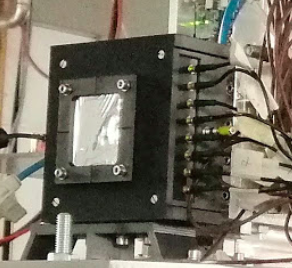
\includegraphics[width=\textwidth, scale=0.5]{2_STreal.png}
			\caption{Foto dello scintillatore SC.}
			\label{fig:start_counter}
		\end{subfigure}
		\hfill
		\begin{subfigure}[t]{0.49\textwidth}
			\centering
			\includegraphics[width=\textwidth, scale=0.5]{beam_monitor.jpg}
			\caption{Particolare interno della camera a drift del BM.}
			\label{fig:beam_monitor}
		\end{subfigure}
		\caption{Schematizzazione della strumentazione dell'upper region \cite{slide_spighi}.}
	\end{figure}
	
	\subsubsection{Tracking region}\label{par:tracking_region}
	Il Vertex (VTX, \hyperref[fig:vtx]{Fig. 2.4a}) viene posizionato subito dopo il target per ricostruire non solo la traiettoria dei frammenti, ma anche per determinare il punto di origine della frammentazione (VTX Point). Il VTX è costituito da quattro piani (di area attiva $2\times2\mbox{ cm}^2$ ciascuno) formati da uno strato di sensori basati sulla tecnologia MAPS.\footnote{Monolithic Active Pixel Sensors, gamma ampiamente usata in imaging ottico, a raggi X e nella detezione di particelle cariche pesanti.} Ciascun pannello è composto da un chip M$28$\footnote{Tali chip riescono a minimizzare ulteriori eventi di \hyperref[par:scattering_Rutherford]{multiple scattering} e frammentazione nucleare dovuti all'interazione delle particelle con l'apparato di misura.} della famiglia dei CMOS formato da una matrice $928\times960$ di pixel al silicio, questi ultimi aventi un passo di $20.7\mbox{ }\mu\mbox{m}$. Ogni pixel prevede un sistema di amplificazione e un circuito CDS (Correlated Double Sampling) di acquisizione con cui è possibile ottenere una risoluzione spaziale del VTX dell'ordine di $5\mbox{ }\mu\mbox{m}$ \cite{foot_cdr,ridolfiArticle}.
	
	Dopo il VTX i frammenti prodotti nel target vengono deviati grazie a uno spettrometro magnetico con cui è possibile valutare la loro quantità di moto. Sebbene la grandezza dello spettrometro sia limitata, il suo potere di deflessione è elevato grazie all'impiego di due magneti dipoli permanenti di Samario-Cobalto (\ce{SmCO}) in configurazione Halbach\footnote{Tale configurazione permette di avere un campo magnetico nullo e uniforme rispettivamente all'esterno e all'interno (nella cavità attraversata dalla traccia) dello spettrometro magnetico.} a geometria cilindrica cava (illustrata in \hyperref[fig:magnetic_spectrometer]{Fig. 2.4b}), grazie alla quale è possibile raggiungere valori massimi di campo magnetico pari a $1.4\mbox{ T}$. Per determinare il momento $p$ dei frammenti, si sfrutta l'espressione della forza di Lorentz $\vect{F_L}$ (\hyperref[eq:lorentz_force]{Eq. 2.4a}) esercitata dal campo magnetico uniforme $\vect{B}$ presente all'interno dello spettrometro magnetico sui frammenti di carica $q$, velocità $\vect{v}$ e massa $m$. Essendo la $\vect{F_L}$ centripeta, è possibile esplicitare la \hyperref[eq:centripetal_force]{Eq. 2.4b}:
	\begin{subequations}
		\begin{align}
			\label{eq:lorentz_force}
			\vect{F_L}&=q\vect{v}\times\vect{B}\\
			\label{eq:centripetal_force}
			\left|\vect{F_L}\right|&=m\frac{v^2}{R}
		\end{align}
	\end{subequations}
	dove $R$ è il raggio di curvatura del frammento dovuto alla sua deflessione magnetica. Confrontando le \hyperref[eq:lorentz_force]{Eq. 2.4a} ed \hyperref[eq:centripetal_force]{Eq. 2.4b}, definendo il modulo dell'impulso $p=mv$ e l'angolo di deflessione delle particelle $\theta$ e sfruttando l'approssimazione valida per piccoli angoli $\sin{\theta}\approx\theta$, è possibile ricavare $p$ in funzione di $\theta$:
	\begin{equation}
		p=\frac{qBL}{\theta}
		\label{eq:momentum_deflession}
	\end{equation}
	dove $L$ è la lunghezza della regione di campo magnetico attraversata. La geometria della deflessione, grazie alla quale è possibile determinare la \hyperref[eq:momentum_deflession]{Eq. 2.5}, è schematizzata in \hyperref[fig:momentum_deflession]{Fig. 2.5}.
	
	Come già proposto nel progetto PLUME \cite{articleNomerotski}, nell'intercapedine dei due magneti si trova l'Inner Tracker (ITR), un rivelatore caratterizzato dalla medesima tecnologia e struttura del VTX (ciò semplifica il sistema di acquisizione dati DAQ) ma dotato di soli due piani di sensori (pixel al silicio) ortogonali alla direzione del fascio entrante. Ciascun piano è formato da $16$ sensori M$28$ (ciascuno dei quali copre una superficie di $2\times2\mbox{ cm}^2$) tenuti da un'impalcatura metallica che prevede un modulo ogni quattro sensori; questi ultimi sono legati assieme su una FPC (Flexible Printed Cable) in Kapton dotata di uno spessore complessivo di $100\mbox{ }\mu\mbox{m}$ (si veda \hyperref[fig:itr]{Fig. 2.4c}). L'ITR è utile a misurare sia la posizione che la direzione della traccia dopo la deviazione prodotta dal primo magnete permanente \cite{foot_cdr,ridolfiArticle}.
	\begin{figure}[H]
		\centering
		\subfloat[Foto del VTX \cite{foot_cdr}.]{\label{fig:vtx}\includegraphics[width=.49\linewidth]{vtx.jpg}}\hfill
		\subfloat[Configurazione Halbach 3D di due magneti simulata con la versione $16$R$1$ del software OPERA \cite{foot_cdr}.]{\label{fig:magnetic_spectrometer}\includegraphics[width=.49\linewidth]{magnetic_spectrometer.jpg}}\par
		\subfloat[Schematizzazione dell'ITR \cite{foot_cdr}.]{\label{fig:itr}\includegraphics[width=.49\linewidth]{itr.jpg}}\hfill
		\subfloat[Foto del MSD \cite{slide_spighi}.]{\label{fig:msd}\includegraphics[width=.49\linewidth]{msd.jpg}}
		\caption{Schematizzazione della strumentazione della tracking region.}
	\end{figure}
	Per tracciare il passaggio dei frammenti dopo la deflessione subita dal secondo magnete permanente, si utilizza il Microstrip Silicon Detector (MSD, \hyperref[fig:msd]{Fig. 2.4d}), un rivelatore formato da tre piani (di area attiva $9.6\times9.3\mbox{ cm}^2$), ciascuno dei quali è costruito da due strati di strisce ortogonali al silicio spesse $70\mbox{ }\mu\mbox{m}$ e tenute assieme da una lamina biadesiva in Kapton spessa $30\mbox{ }\mu\mbox{m}$. La soluzione a due strati è stata preferita rispetto a quella di un unico piano (spesso $150\mbox{ }\mu\mbox{m}$) poiché nel primo modo è possibile ottenere due misure di $\frac{dE}{dx}$ indipendenti e una rigidità meccanica del MSD maggiore. Nonostante ciò, a differenza dei pixel, le strisce al silicio potrebbero produrre ambiguità nell'identificazione della posizione dei frammenti, eventualmente risolte attraverso un'analisi del fondo combinatoriale dei segnali prodotti dai frammenti.\footnote{Analizzando la potenza dei segnali elettrici rilasciati nel rivelatore, è possibile associare a questi ultimi la particella che li ha generati.} La risoluzione spaziale dell'MSD è di circa $40\mbox{ }\mu\mbox{m}$ \cite{foot_cdr,ubaldiArticle}.
	\begin{figure}[H]
		\centering
		\includegraphics[width=0.8\linewidth]{momentum_deflession.pdf}
		\caption{Schematizzazione della deflessione subita da una particella carica in una regione di campo magnetico uniforme \cite{leoniS}.}
		\label{fig:momentum_deflession}
	\end{figure}
	
	\subsubsection{Downstream region}\label{par:downstream_region}
	Il TOF Wall (TW, \hyperref[fig:tw]{Fig. 2.6a}) è uno scintillatore (di area attiva $40\times40\mbox{ cm}^2$) formato da due strati ortogonali di $20$ barre ciascuno. Ogni barra è spessa $0.3\mbox{ cm}$ ed è accoppiata a ogni estremità con $4$ SiPM, grazie ai quali è possibile ricostruire l'energia depositata per unità di lunghezza $\left(\frac{dE}{dx}\right)$\footnote{Per misurare il $dE/dx$ dei frammenti, il TW assorbe una parte della loro energia $\Delta E$ che, in seguito, viene aggiunta al computo totale della loro energia cinetica.} con una precisione $\approx5\%$. Inoltre, quando i frammenti giungono al TW, viene fermato il TOF (il cui istante iniziale viene dato dallo SC). Grazie al TOF e alla traiettoria dei frammenti (ricostruita tramite VTX, ITR e MSD) si può ricavare la loro velocità $\beta$ che, unita al $\frac{dE}{dx}$, consente di ricostruire la carica dei frammenti ($z$) tramite la \hyperref[eq:bethe_bloch]{Eq. 1.35}.
	\begin{figure}[H]
		\centering
		\subfloat[Foto di una superificie del TW.]{\label{fig:tw}\includegraphics[width=.49\linewidth]{tw.jpg}}\hfill
		\subfloat[Schema di uno dei cristalli BGO del CALO, alla cui estremità sono situati dei SiPM.]{\label{fig:calo}\includegraphics[width=.49\linewidth]{calo.jpg}}
		\par
		\subfloat[Calibrazione della posizione dei cristalli BGO del CALO.]{\label{fig:calo2}\includegraphics[width=.39\linewidth]{calo2.jpg}}
		\caption{Schematizzazione della strumentazione della downstream region \cite{slide_spighi}.}
	\end{figure}
	Il Calorimetro (CALO) è uno scintillatore inorganico costituito da cristalli di BGO (bismuto \ce{Bi}, germanio \ce{Ge} e ossigeno \ce{O}, si vedano le \hyperref[fig:calo]{Fig. 2.6b} e \hyperref[fig:calo2]{Fig. 2.6c}), oggetti caratterizzati da alta densità ed elevati numeri atomici, proprietà che rendono tale rivelatore molto pesante ($\approx330\mbox{ kg}$). Quando i frammenti penetrano nel CALO, data l'elevata densità atomica dei cristalli BGO, si producono principalmente interazioni elettromagnetiche che portano all'emissione di fotoni e alla perdita di tutta l'energia $E$ dei frammenti stessi. La quantità di luce prodotta all'interno del CALO, misurata tramite dei SiPM posti nella parte terminale dei cristalli BGO, è proporzionale all'energia cinetica $E_k$ dei frammenti (misurata con una risoluzione dell'$1$--$2\%$). All'interno del CALO i frammenti possono andare incontro anche a interazioni nucleari, la cui presenza influenza notevolmente la misura dell'energia $E$ rilasciata nello strumento. Infatti, nel $10$--$20\%$ degli eventi, le interazioni nucleari portano alla formazioni di neutroni, i quali fuoriescono dal CALO senza essere rivelati dai SiPM. Ciò genera una sottostima sistematica dell'energia totale rilasciata (a cui consegue una sottostima o una sovrastima della massa dei frammenti nel caso in cui quest'ultima venga ricavata rispettivamente dalla \hyperref[eq:a2]{Eq. 2.3b} o dalla \hyperref[eq:a3]{Eq. 2.3c}, uniche equazioni della massa in cui compare l'$E_k$ misurata dal CALO). Tale effetto, più pronunciato per i frammenti più leggeri, può essere limitato per mezzo di misurazioni multiple e indipendenti della massa dei frammenti prodotti \cite{foot_cdr}.
	
	\subsection{Camera a emulsione}
	\begin{figure}[H]
		\centering
		\includegraphics[width=0.5\linewidth]{position_es.jpg}
		\caption{Localizzazione dell'ES all'interno dell'apparato sperimentale di FOOT \cite{foot_cdr}.}
		\label{fig:position_es}
	\end{figure}
	Sebbene le camere a emulsione siano state superate dai rivelatori elettronici sin dagli anni sessanta \cite{Ariga2020}, sono dispositivi utilizzati ancora oggi nella fisica delle particelle per motivi quali la loro compattezza, l'elevata accuratezza e velocità con cui è possibile ricostruire le interazioni che avvengono nel target, la capacità di integrare bersaglio e rivelatori in un unico setup e, come già accennato, l'elevata accettanza angolare. Prima di FOOT, nel contesto della frammentazione nucleare, si ebbe un'esperienza delle camere a emulsione all'HIMAC di Chiba (si veda \hyperref[sec:storia_adroterapia]{Sez. 1.3.1}), dove per studiare la frammentazione di ioni \ce{^{12}C} a $400\mbox{ MeV/u}$ si impiegò un rivelatore composto da strati alternati di policarbonato (Lexan, per simulare i tessuti umani) e film a emulsione \cite{articleNakamura,articleLellis1,articleLellis2}.
	
	La camera a emulsione (o Spettrometro a Emulsione, ES) dell'esperimento FOOT è utilizzata per la rivelazione dei frammenti nucleari più leggeri, il cui angolo di diffusione ($\approx70^\circ$) risulta troppo elevato rispetto all'accettanza angolare del setup elettronico.\footnote{La scelta della camera a emulsione risiede nel fatto che calorimetri con accettanze angolari di $\approx70^\circ$ sono difficili da realizzare per problemi di portabilità e per questioni economiche.} L'ES di FOOT, posizionato dopo lo Start Counter e il Beam Monitor (si veda \hyperref[fig:position_es]{Fig. 2.7}), è costituito da una stratificazione di film che fungono da bersaglio, formati da materiali passivi (come il \ce{C} o il \ce{C2H4}), alternati a pellicole a emulsione nucleare di bromuro d'argento (\ce{AgBr}), la cui eccitazione energetica (dovuta al rilascio di energia dei frammenti nucleari) consente di tracciare il passaggio delle particelle incidenti. L'analisi delle tracce avviene tramite un sistema di scanning automatico (basato su un microscopio ottico) già adottato nell'esperimento OPERA \cite{Armenise:2005yh,Arrabito:2006rv} e nel progetto FIRST\footnote{Fragmentation of Ions Relevant for Space and Therapy.} \cite{PhysRevC.93.064601}.
	\begin{figure}[H]
		\centering
		\includegraphics[width=0.9\linewidth]{structure_es.pdf}
		\caption{Schema della struttura dell'ES dell'esperimento FOOT \cite{foot_cdr}.}
		\label{fig:structure_es}
	\end{figure}
	L'ES è composto da tre sezioni, la cui struttura è schematizzata in \hyperref[fig:structure_es]{Fig. 2.8}:
	\begin{itemize}
		\item regione di vertexing: profonda $\approx4\mbox{ cm}$, è formata da strati di \ce{C} o \ce{C2H4} (i bersagli dell'esperimento) profondi $\approx1\mbox{ mm}$ alternati a film a emulsione dello spessore di $300\mbox{ }\mu{m}$.
		\item regione di ionizzazione: profonda $\approx1\mbox{ cm}$, è costituita da celle elementari, ciascuna contenente tre film a emulsione dotate di sensibilità particellari differenti. Grazie ai film a emulsione è possibile identificare la carica di frammenti leggeri (con un'efficienza molto alta, pari a $\approx90\%$) come \ce{H}, \ce{He} e \ce{Li} \cite{deLellisConference}.
		\item regione di tracciamento: profonda $\approx4\mbox{ cm}$, è costituita da film a emulsione spessi $300\mbox{ }\mu{m}$ intervallati a strati di piombo (\ce{Pb}) di profondità $1\mbox{ mm}$. Misurando la lunghezza totale del range dei frammenti, è possibile determinare sia la loro energia cinetica che la loro quantità di moto.\footnote{Ciò avviene tramite una relazione tra range e quantità di moto prevista dal modello a Multiple Coulomb Scattering \cite{articleAgafonova,DESERIO2003539}.}
	\end{itemize}
	
	\chapter{Identificazione dei frammenti}\label{cap:3}
	Dopo aver esposto le principali caratteristiche strutturali e di funzionamento del setup sperimentale di FOOT nel \hyperref[cap:2]{Cap. 2}, nel \hyperref[cap:3]{Cap. 3} si propone un'analisi più tecnica delle attività di ricerca sviluppate nell'esperimento. Oltre allo sviluppo hardware accennato nel \hyperref[cap:2]{Cap. 2} (che prevede, tra i vari compiti, quello di impiegare sofisticati sistemi di DAQ con cui acquisire grandi quantità di dati con la maggiore accuratezza possibile), in FOOT si utilizza un programma basato sul framework ROOT \cite{rene_brun}, sviluppato per la prima volta durante il progetto FIRST \cite{foot_cdr}. Tale programma è dotato di algoritmi di ricostruzione e di identificazione della traccia (come il filtro Kalman, implementato nella libreria GENFIT \cite{Rauch_2015}, utile a trovare la miglior stima dello stato cinematico dei frammenti) con cui si possono analizzare sia eventi simulati (tramite simulazioni Monte Carlo fornite da FLUKA o ROOT) sia dati reali. Prima di ottenere il fit finale da cui estrarre i parametri della traccia (come energia, momento, direzione, etc.), si attuano varie strategie di ricostruzione della traccia sviluppate a partire dall'analisi combinata dei segnali raccolti nel setup sperimentale; naturalmente, tali tecniche tengono conto delle perdite di energia e dei processi di scattering che avvengono nei rivelatori e della deflessione delle particelle cariche dovuta al campo magnetico \cite{ridolfiArticle}.
	
	\section{Analisi preliminare}\label{sec:fragment_identification}
	Prima di misurare la sezione d'urto dei frammenti secondari prodotti dalla frammentazione del target o del proiettile a causa delle interazioni nucleari delle particelle cariche, è necessario identificare suddetti frammenti. A tale scopo, occorre determinare il loro numero atomico $Z$ e di massa $A$ a partire dalle grandezze fisiche misurate dai rivelatori, come già descritto in dettaglio nella \hyperref[sec:setupElettronico]{Sez. 2.2.1}. Riassumendo, tali grandezze derivano dalle misure di tempo di volo (TOF), di quantità di moto $p$, di rilascio di energia del frammento all'interno del TW $\Delta E_{TW}$ e di energia cinetica $E_k$. Nello specifico, il TOF viene misurato sottraendo all'intervallo di tempo che intercorre tra i segnali di SC e TW il tempo necessario al fascio per percorrere la distanza tra lo SC e il target; si dimostra che la sua risoluzione diminuisce all'aumentare dell'energia depositata dalle particelle nei rivelatori, dunque è di $\approx200$--$250\mbox{ ps}$ per i frammenti più leggeri e $\approx50$--$70\mbox{ ps}$ per quelli più pesanti \cite{foot_cdr}. La misura di $p$ avviene nella tracking region grazie alla deflessione subita dalle particelle nella regione di campi magnetici, e la sua risoluzione percentuale è inferiore al $3\%$ \cite{foot_cdr}. L'energia cinetica $E_k$ è data dalla somma delle energie depositate nell'MSD $\Delta E_{MSD}$, nel TW $\Delta E_{TW}$ e nel CALO $\Delta E_{CALO}$:
	\begin{equation}
		E_k=\Delta E_{MSD}+\Delta E_{TW}+\Delta E_{CALO}
		\label{eq:deposited_energy}
	\end{equation}
	In realtà la $\Delta E_{MSD}$ dell'\hyperref[eq:deposited_energy]{Eq. 3.1} rappresenta una piccola perturbazione alle energie $\Delta E_{TW}$ e $\Delta E_{CALO}$, pertanto nel prosieguo dell'analisi verrà trascurata. $\Delta E_{TW}$ e $\Delta E_{CALO}$ possiedono una risoluzione pari rispettivamente al $3$--$10\%$ e all'$1.5\%$ \cite{foot_cdr}. Dunque, trascurando la $\Delta E_{MSD}$, si ottiene $E_k=\Delta E_{TW}+\Delta E_{CALO}$, da cui è possibile stimare $E_k$ e la sua risoluzione.
	
	Le risoluzioni di $Z$ e di $A$, oltre a essere dipendenti dalle sopra citate risoluzioni, sono fortemente legate a due fattori:
	\begin{itemize}
		\item la perdita di energia subita dai frammenti negli eventuali processi di ionizzazione che avvengono prima della loro rivelazione nel CALO;
		\item la perdita di energia subita dai frammenti all'interno del CALO a causa dell'emissione di neutroni, processo già descritto nell'analisi della \hyperref[par:downstream_region]{downstream region} nella \hyperref[sec:setupElettronico]{Sez. 2.2.1}.
	\end{itemize}
	La presenza di tali problematiche supporta ulteriormente la necessità di possedere un apparato di rivelazione ridondante, con cui è possibile ricostruire le stesse grandezze fisiche in modalità differenti.
	
	Nei paragrafi successivi si analizzano dei dati simulati dal software FLUKA, in cui un fascio incidente di $\approx10$ milioni di ioni \ce{^{12}C} di energia cinetica $200\mbox{ MeV/u}$ collide con un target di grafite al \ce{^{12}C} spesso $0.5 \mbox{ mm}$ e distante $29 \mbox{ cm}$ dallo SC. L'analisi è incentrata sullo studio degli isotopi dei frammenti maggiormente prodotti, riassunti in \hyperref[tab:fragments]{Tab. 3.1}.
	\begin{table}[H]
		\begin{minipage}{\textwidth}
			\centering
			\begin{tabular}{ |M{2.2cm}||M{1.5cm}|M{1.5cm}|M{1.5cm}|M{1.5cm}|M{1.5cm}| }
				\hline
				Frammento &\ce{^{1}H}&\ce{^{2}H}&\ce{^{3}He}&\ce{^{4}He}&\ce{^6Li}\\
				\hline
				$Z$ & $1$& $1$& $2$& $2$& $3$\\
				\hline
				$A$ & $1$& $2$ &$3$ &$4$& $6$\\
				\hline
				\hline
				Frammento &\ce{^7Li}&\ce{^7Be}&\ce{^{9}Be}&\ce{^{11}B}&\ce{^{12}C}\\
				\hline
				$Z$ & $3$& $4$& $4$& $5$& $6$\\
				\hline
				$A$ & $7$& $7$ &$9$ &$11$& $12$\\
				\hline
			\end{tabular}
		\end{minipage}
		\caption{Lista degli isotopi dei frammenti secondari maggiormente prodotti con relativi numeri atomici $Z$ e di massa $A$ \cite{foot_cdr}.}
		\label{tab:fragments}
	\end{table}
	
	\section{Identificazione del numero atomico}\label{sec:atomic_number_identification}
	Il numero atomico $Z$ di ciascun frammento secondario viene calcolato all'interno del TW invertendo la formula di Bethe-Bloch (\hyperref[eq:bethe_bloch]{Eq. 1.35}) e trascurando i termini correttivi $\delta$ e $C$, da cui si ottiene la \hyperref[eq:atomic_number]{Eq. 3.2}:
	\begin{equation}
		Z=\sqrt{\frac{4\pi M_u\epsilon_0^2m_ec^2}{N_A\rho e^4}\left(\frac{\overline{Z}}{A}\right)^{-1}\frac{dE}{dx}\frac{\beta^2}{\ln{\left[\frac{2m_ec^2\beta^2}{I\left(1-\beta^2\right)}\right]}-\beta^2}}
		\label{eq:atomic_number}
	\end{equation}
	i cui parametri sono riassunti in \hyperref[tab:bethe_bloch]{Tab. 1.3}, dove al posto di $z$ e $Z$ vengono utilizzati per convenzione $Z$ e $\overline{Z}$. In particolare, $\beta$ (che in questo caso è la velocità del frammento) si ricava dalla seguente espressione:
	\begin{equation}
		\beta=\frac{v}{c}=\frac{L}{TOF\cdot c}
		\label{eq:beta_beam}
	\end{equation}
	dove $L$, $v$ e $TOF$ sono rispettivamente la distanza percorsa, la velocità e il TOF del frammento secondario. $L$ viene ricostruita da un algoritmo che seleziona i segnali di posizione raccolti al passaggio dei frammenti, a partire dal primo strato del VTX fino all'ultima barra di scintillatore del TW. I parametri $\rho$, $\frac{\overline{Z}}{A}$ e $I$ della \hyperref[eq:atomic_number]{Eq. 3.2} sono relativi all'EJ-$200$, materiale plastico formato da polimeri di poliviniltoluene (PVT) che costituisce le barre di scintillatore del TW \cite{pvt}. Inoltre, trascurando l'energia rilasciata nell'MSD, è possibile valutare il potere frenante $\frac{dE}{dx}$ utilizzando l'energia depositata nelle due barre di scintillatore del TW $\Delta E_{TW}$ e il loro spessore $\Delta x$, come riassunto nella \hyperref[eq:stopping_power]{Eq. 3.4}:
	\begin{equation}
		\frac{dE}{dx}=\frac{\Delta E_{TW}}{\Delta x}
		\label{eq:stopping_power}
	\end{equation}
	Dalle \hyperref[eq:atomic_number]{Eq. 3.2}, \hyperref[eq:beta_beam]{Eq. 3.3} ed \hyperref[eq:stopping_power]{Eq. 3.4} si ricavano sia la distribuzione di $Z$, rappresentata in \hyperref[fig:atomic_numbersa]{Fig. 3.1a}, sia la distribuzione di $\Delta E_{TW}$ in funzione del TOF, raffigurata in \hyperref[fig:atomic_numbersb]{Fig. 3.1b}.
	
	In entrambe le \hyperref[fig:atomic_numbersa]{Fig. 3.1a} e \hyperref[fig:atomic_numbersb]{Fig. 3.1b} si distinguono dei picchi che consentono una chiara identificazione della carica dei frammenti. Le migliori stime di $Z$, ricavate dai fit gaussiani in \hyperref[fig:atomic_numbersa]{Fig. 3.1a}, sono riassunte in \hyperref[tab:atomic_numbers_a]{Tab. 3.2} e \hyperref[tab:atomic_numbers_b]{Tab. 3.3}. Tali misure sono caratterizzate da una risoluzione che va dal $5.3\%$ dell'\ce{H} al $2.3\%$ del \ce{C} e presentano uno shift rispetto ai valori attesi. Dalle \hyperref[tab:atomic_numbers_a]{Tab. 3.2} e \hyperref[tab:atomic_numbers_b]{Tab. 3.3} si osserva che le misure di $Z$ dei frammenti sono tutte compatibili con i valori attesi entro le incertezze sperimentali.
	\begin{table}[H]
		\begin{minipage}{\textwidth}
			\centering
			\begin{tabular}{ |M{3.5cm}||M{3.cm}|M{3.cm}|M{3.cm}| }
				\hline
				Frammento &\ce{H}&\ce{He}&\ce{Li}\\
				\hline
				$Z$ atteso & $1$& $2$& $3$\\
				\hline
				$Z$ ricostruito & $1.001\pm0.053$& $2.017\pm0.077$ &$3.00\pm0.12$\\
				\hline
			\end{tabular}
		\end{minipage}
		\caption{Ricostruzione delle migliori stime dei numeri atomici $Z\le3$ dei frammenti considerati, le cui incertezze sono pari alla $\sigma$ dei fit gaussiani evidenziati in \hyperref[fig:atomic_numbers]{Fig. 3.1}.}
		\label{tab:atomic_numbers_a}
	\end{table}
	\begin{table}[H]
		\begin{minipage}{\textwidth}
			\centering
			\begin{tabular}{ |M{3.5cm}||M{3.cm}|M{3.cm}|M{3.cm}| }
				\hline
				Frammento &\ce{Be}&\ce{B}&\ce{C}\\
				\hline
				$Z$ atteso & $4$& $5$& $6$\\
				\hline
				$Z$ ricostruito & $4.02\pm0.13$& $5.05\pm0.13$ &$6.08\pm0.14$ \\
				\hline
			\end{tabular}
		\end{minipage}
		\caption{Ricostruzione delle migliori stime dei numeri atomici $Z>3$ dei frammenti considerati, le cui incertezze sono pari alla $\sigma$ dei fit gaussiani evidenziati in \hyperref[fig:atomic_numbers]{Fig. 3.1}.}
		\label{tab:atomic_numbers_b}
	\end{table}
	\begin{figure}[H]
		\centering
		\begin{subfigure}[t]{1.\textwidth}
			\centering
			\includegraphics[width=\textwidth, scale=0.50]{c_z.pdf}
			\caption{Distribuzione di $Z$ determinata a partire dalla \hyperref[eq:atomic_number]{Eq. 3.2} e relativi fit. Dalla rappresentazione è esclusa la distribuzione centrata in $Z=6$ del \ce{C}.}
			\label{fig:atomic_numbersa}
		\end{subfigure}
		\par
		\begin{subfigure}[t]{1.\textwidth}
			\centering
			\includegraphics[width=\textwidth, scale=0.50]{c_E_TOF.pdf}
			\caption{Distribuzione di $\Delta E_{TW}$ in funzione del TOF.}
			\label{fig:atomic_numbersb}
		\end{subfigure}
		\caption{Distribuzioni utilizzate per l'identificazione del numero atomico $Z$ dei frammenti secondari considerati.}
		\label{fig:atomic_numbers}
	\end{figure}
	
	\section{Identificazione del numero di massa}
	La ridondanza del \hyperref[sec:setupElettronico]{setup elettronico} di FOOT consente di determinare il numero di massa $A$ in modi differenti. In particolare, le misure di TOF, di $p$ e di $E_k$ si possono combinare in tre modi differenti in modo da ottenere tre stime di $A$: $A_1$, $A_2$ e $A_3$. Tali stime si ottengono:
	\begin{itemize}
		\item attraverso la \hyperref[eq:a1]{Eq. 2.3a}, in cui si determinano $\beta$ e $p$ rispettivamente dal TOF e dalla tracking region;
		\item attraverso la \hyperref[eq:a2]{Eq. 2.3b}, in cui si determinano $\beta$ e $E_k$ rispettivamente dal TOF e dal CALO;\footnote{Si ricorda che $E_k$ dipende anche dai contributi energetici del TW e dell'MSD, anche se in maniera molto minore rispetto al CALO.}
		\item attraverso la \hyperref[eq:a3]{Eq. 2.3c}, in cui si determinano $p$ e $E_k$ rispettivamente dalla tracking region e dal CALO.
	\end{itemize}
	$A_1$, $A_2$ e $A_3$ non sono stime indipendenti poiché, prese a due a due, sono legate a grandezze fisiche misurate con il medesimo sub-detector. Determinare la correlazione tra $A_1$, $A_2$ e $A_3$ costituisce una parte fondamentale dell'analisi dei dati di FOOT, con la quale è possibile valutare la miglior stima di $A$ e la relativa incertezza. Per analizzare la correlazione tra $A_1$, $A_2$ e $A_3$, solitamente si utilizzano due procedure algebriche, ossia il metodo del minimo $\chi^2$ e l'Augmented Lagrangian Method. Tali tecniche si basano sulla minimizzazione di una funzione a più variabili. In questa tesi, invece, il problema della correlazione tra $A_1$, $A_2$ e $A_3$ viene affrontato dal punto di vista grafico, a partire dalla \hyperref[sec:correlation_number_mass]{Sez. 3.3.1}.
	
	\subsection{Correlazione dei numeri di massa}\label{sec:correlation_number_mass}
	Per analizzare la correlazione tra i numeri di massa $A_1$, $A_2$ e $A_3$ dei frammenti secondari selezionati, si rappresentano degli istogrammi bidimensionali i cui assi coordinati contengono tutte le possibili combinazioni di $A_1$, $A_2$ e $A_3$. Per ciascun frammento, in \hyperref[fig:a1]{Fig. 3.2} viene rappresentata la correlazione tra $A_1$ e $A_2$, in \hyperref[fig:a2]{Fig. 3.3} quella tra $A_1$ e $A_3$ e in \hyperref[fig:a3]{Fig. 3.4} quella tra $A_2$ e $A_3$. Nelle \hyperref[fig:a1]{Fig. 3.2}, \hyperref[fig:a2]{Fig. 3.3} e \hyperref[fig:a3]{Fig. 3.4} si osservano dei picchi la cui dispersione è dovuta alle differenti risoluzioni delle grandezze fisiche di TOF, $p$ ed $E_k$, già discusse nell'introduzione della \hyperref[sec:fragment_identification]{Sez. 3.1}. In corrispondenza dei picchi si possono ricostruire gli isotopi dei frammenti maggiormente prodotti. Oltre alle regioni di picco, poste chiaramente in prossimità della bisettrice di ogni istogramma, vi sono delle occorrenze situate lontano dalla bisettrice le cui distribuzioni assumono andamenti specifici per ogni figura rappresentata.
	\begin{figure}[H]
		\centering
		\includegraphics[width=1.03\linewidth,center]{c_MultiCanvas1.pdf}
		\caption{Rappresentazione della correlazione tra i numeri di massa $A_1$ e $A_2$.}
		\label{fig:a1}
	\end{figure}
	Dalla \hyperref[fig:a1]{Fig. 3.2} si nota che in corrispondenza dei picchi un certo numero di occorrenze genera delle code orientate orizzontalmente e, soprattutto, verticalmente. Infatti, le code con maggiore densità di eventi si sviluppano a partire dai picchi e procedono verticalmente verso il basso, suggerendo che le distribuzioni di $A_2$ presentino una sottostima.
	\begin{figure}[H]
		\centering
		\includegraphics[width=1.03\linewidth,center]{c_MultiCanvas2.pdf}
		\caption{Rappresentazione della correlazione tra i numeri di massa $A_1$ e $A_3$.}
		\label{fig:a2}
	\end{figure}
	Dalla \hyperref[fig:a2]{Fig. 3.3} si osservano delle code che, a differenza della \hyperref[fig:a1]{Fig. 3.2}, si sviluppano verticalmente nella parte superiore dei picchi, suggerendo che le distribuzioni di $A_3$ presentino una sovrastima.
	\begin{figure}[H]
		\centering
		\includegraphics[width=1.03\linewidth,center]{c_MultiCanvas3.pdf}
		\caption{Rappresentazione della correlazione tra i numeri di massa $A_2$ e $A_3$.}
		\label{fig:a3}
	\end{figure}
	Nella \hyperref[fig:a3]{Fig. 3.4} le occorrenze, oltre a distribuirsi nei picchi, assumono un andamento quasi iperbolico. Nello specifico, si nota che la parte delle code più popolate è quella che dai picchi si sviluppa in alto a sinistra, confermando che le distribuzioni di $A_2$ e $A_3$ presentano rispettivamente una sottostima e una sovrastima come già osservato per le \hyperref[fig:a1]{Fig. 3.2} e \hyperref[fig:a2]{Fig. 3.3}.
	
	La differenza degli andamenti delle distribuzioni in \hyperref[fig:a1]{Fig. 3.2}, \hyperref[fig:a2]{Fig. 3.3} e \hyperref[fig:a3]{Fig. 3.4} risiede nel fatto che ogni distribuzione si ricava da un sub-detector comune alla coppia dei numeri di massa analizzati o, equivalentemente, dalla medesima grandezza fisica. Infatti, le coppie $A_1$--$A_2$ possiedono in comune la misura della velocità $\beta$ dei frammenti, quindi è possibile pensare che l'andamento della loro distribuzione rappresenti il legame funzionale implicito delle grandezze fisiche non correlate delle \hyperref[eq:a1]{Eq. 2.3a} ed \hyperref[eq:a2]{Eq. 2.3b}, ossia $p$ ed $E_k$. Allo stesso modo, le occorrenze $A_1$--$A_3$ condividono la misura del momento $p$ dei frammenti, dunque la loro distribuzione rivela la relazione funzionale tra $\beta$ ed $E_k$. Infine, visto che per ricavare le $A_1$--$A_3$ sono necessarie le misure di energia cinetica $E_k$ dei frammenti, la loro distribuzione descrive il legame implicito tra $p$ e $\beta$.
	
	L'andamento quasi iperbolico delle coppie $A_1$--$A_3$ in \hyperref[fig:a3]{Fig. 3.4} si distingue dagli altri poiché le misure di $E_k$ risultano particolarmente problematiche a causa delle perdite di energia subite dai frammenti nel loro percorso. Infatti, come già discusso nel paragrafo della \hyperref[par:downstream_region]{downstream region} nel \hyperref[cap:2]{Cap. 2}, la maggiore perdita di $E_k$ si ha nel CALO, ed è causata dall'emissione di neutroni che sfuggono alle interazioni con i cristalli BGO del rivelatore, effetto che induce una diminuzione dei valori di $E_k$.
	
	Inoltre, osservando la dipendenza funzionale delle \hyperref[eq:a1]{Eq. 2.3a} ed \hyperref[eq:a2]{Eq. 2.3b} rispetto alla variabile $E_k$, si può notare che a una diminuzione di $E_k$ corrispondono un abbassamento di $A_2$ e un aumento di $A_3$. Pertanto, le perdite di energia unite alle \hyperref[eq:a1]{Eq. 2.3a} ed \hyperref[eq:a2]{Eq. 2.3b} spiegano il motivo per cui le code delle distribuzioni di $A_2$ e $A_3$ abbiano sempre due shift opposti in tutti gli istogrammi bidimensionali.
	
	\subsection{Selezione dei numeri di massa}\label{sec:selection_number_of_mass}
	Per procedere con l'analisi dei dati dei numeri di massa, si selezionano le occorrenze più significative delle \hyperref[fig:a1]{Fig. 3.2}, \hyperref[fig:a2]{Fig. 3.3} e \hyperref[fig:a3]{Fig. 3.4}, ossia quelle che si trovano in un intorno della bisettrice degli istogrammi bidimensionali. Per attuare la selezione, in ciascun istogramma sono rappresentate due rette vicine alla bisettrice. Successivamente, vengono estrapolate tutte le occorrenze situate entro la regione di piano definita dalle due rette di taglio. La selezione delle occorrenze in \hyperref[fig:a1]{Fig. 3.2}, \hyperref[fig:a2]{Fig. 3.3} e \hyperref[fig:a3]{Fig. 3.4} è riportata rispettivamente nelle \hyperref[fig:a1_cut]{Fig. 3.5}, \hyperref[fig:a2_cut]{Fig. 3.6} e \hyperref[fig:a3_cut]{Fig. 3.7}.
	\begin{figure}[H]
		\centering
		\includegraphics[width=1.0\linewidth]{c_MultiCanvasCut1.pdf}
		\caption{Rappresentazione della correlazione tra i numeri di massa $A_1$ e $A_2$ con le relative funzioni di taglio utilizzate per la selezione delle occorrenze significative.}
		\label{fig:a1_cut}
	\end{figure}
	La selezione grafica delle occorrenze più significative si rivela piuttosto efficace nel ``ripulire'' i dati di $A_1$, $A_2$ e $A_3$ dagli shift indotti dalle perdite di energia e, più in generale, dalle dispersioni generate dalle occorrenze presenti nelle code degli istogrammi bidimensionali. Ciò permette di ottenere delle stime di $A_1$, $A_2$ e $A_3$ più accurate, come verrà evidenziato nel prosieguo.
	\begin{figure}[H]
		\centering
		\includegraphics[width=1.03\linewidth,center]{c_MultiCanvasCut2.pdf}
		\caption{Rappresentazione della correlazione tra i numeri di massa $A_1$ e $A_3$ con le relative funzioni di taglio utilizzate per la selezione delle occorrenze significative.}
		\label{fig:a2_cut}
	\end{figure}
	Grazie alle funzioni di taglio delle \hyperref[fig:a1_cut]{Fig. 3.5}, \hyperref[fig:a2_cut]{Fig. 3.6} e \hyperref[fig:a3_cut]{Fig. 3.7} è possibile limitare un'ulteriore problematica dovuta all'algoritmo di ricostruzione del setup sperimentale di FOOT. Per comprenderla, occorre ricordare il funzionamento della \hyperref[par:tracking_region]{tracking region} esposto nella \hyperref[sec:setupElettronico]{Sez. 2.2.1}, in cui si descrive che la misura della quantità di moto $p$ dei frammenti si ottiene analizzando la curvatura della loro traiettoria, dovuta alla deflessione prodotta dal campo magnetico. In realtà, la grandezza fisica effettivamente misurata nella \hyperref[par:tracking_region]{tracking region} non è $p$ ma è la rigidità $\frac{p}{Z}$, dove $Z$ è la carica del frammento. Dunque, la misura della quantità di moto dei frammenti è strettamente correlata all'identificazione di $Z$ che, dalla \hyperref[sec:atomic_number_identification]{Sez. 3.2}, avviene tramite il rilascio di energia nelle barre di scintillatore del TW.
	\begin{figure}[H]
		\centering
		\includegraphics[width=.95\linewidth]{c_MultiCanvasCut3.pdf}
		\caption{Rappresentazione della correlazione tra i numeri di massa $A_2$ e $A_3$ con le relative funzioni di taglio utilizzate per la selezione delle occorrenze significative.}
		\label{fig:a3_cut}
	\end{figure}
	Il problema sopra citato fa riferimento alla possibilità che hanno i frammenti di andare incontro a frammentazione nucleare in una regione differente dal target. In generale, l'algoritmo di ricostruzione di FOOT esclude dall'analisi la maggior parte degli eventi in cui la frammentazione non è avvenuta nel target, ma quando ciò non avviene si possono generare degli errori di ricostruzione che necessitano di una corretta interpretazione. Ad esempio, può accadere che un \ce{^{12}C} non subisca frammentazione nel target ma nello spazio ($\approx1\mbox{ m}$) che separa la regione magnetica e il TW. Poniamo che il \ce{^{12}C} frammenti in aria in elementi pesanti come boro \ce{B} o berillio \ce{Be}, poiché si attende che l'artefatto ricostruttivo abbia un impatto maggiore sui frammenti pesanti piuttosto che su quelli leggeri. Infatti, il $\beta$ dei frammenti pesanti è molto simile a quello delle particelle da cui derivano e, dalla \hyperref[fig:angular]{Fig. 2.1}, è noto che la distribuzione angolare dei frammenti più pesanti è molto più piccata ad angoli bassi. Ciò non facilita l'algoritmo di ricostruzione di FOOT, che è più propenso a escludere eventi nel momento in cui velocità e direzione dei frammenti sono differenti da quelli della particella frammentata. Dunque, avendo un numero di massa piuttosto elevato, i frammenti di \ce{B} o \ce{Be} avranno una velocità e una direzione simili a quelle del \ce{^{12}C}, ma la loro carica $Z'$ è chiaramente diversa dalla $Z$ del \ce{^{12}C}. Quindi, ciò che può accadere è che la \hyperref[par:tracking_region]{tracking region} misuri un $\frac{p}{Z}$ relativo al \ce{^{12}C}, mentre il TW riveli la carica $Z'$ corrispondente ai frammenti \ce{B} o \ce{Be}. Ricordando la \hyperref[eq:a1]{Eq. 2.3a}, si ottiene la \hyperref[eq:error_reconstruction]{Eq. 3.5}:
	\begin{equation}
		\frac{p}{Z}=u\beta c\gamma\cdot \frac{A_1}{Z}\propto\frac{A_1}{Z}
		\label{eq:error_reconstruction}
	\end{equation}
	Adattando la \hyperref[eq:error_reconstruction]{Eq. 3.5} all'esempio di cui sopra ed esplicitando $A_1$ si ottiene la \hyperref[eq:error_reconstruction_final]{Eq. 3.6}:
	\begin{equation}
		A_1\propto Z'\cdot\frac{p}{Z}
		\label{eq:error_reconstruction_final}
	\end{equation}
	da cui si può comprendere che una differenza tra $Z$ e $Z'$ induce un errore nella ricostruzione di $A_1$. Sebbene questo tipo di eventi risulti particolarmente evidente per $A_1$, può avvenire anche nella ricostruzione di $A_2$ e $A_3$.
	\subsubsection{Il caso del \ce{^8Be}}
	Come si accennava, grazie alle funzioni di taglio delle \hyperref[fig:a1_cut]{Fig. 3.5}, \hyperref[fig:a2_cut]{Fig. 3.6} e \hyperref[fig:a3_cut]{Fig. 3.7} è possibile limitare la presenza di errori nella ricostruzione del numero di massa dei frammenti. In particolare, dai dati simulati in questa tesi, si può osservare l'azione delle funzioni di taglio sul caso particolarmente esemplare del \ce{^8Be}. Tale isotopo, infatti, non può essere rivelato dall'apparato sperimentale di FOOT per via della sua brevissima vita media di $\approx10^{-16}\mbox{ s}$ \cite{TILLEY2004155}. Nonostante ciò, come si nota dalla \hyperref[fig:berillium1]{Fig. 3.8}, la distribuzione dei valori di $A_1$ presenta un evidente picco in $Z=8$, dovuto necessariamente all'errore di ricostruzione esposto in precedenza. Inoltre, analizzando le \hyperref[fig:berillium2]{Fig. 3.9} e \hyperref[fig:berillium3]{Fig. 3.10}, si osserva che il taglio garantisce non solo l'eliminazione pressoché totale del picco in $A_1=8$ per le misure di $A_1$, ma anche una pulizia maggiore dei dati di $A_2$ e $A_3$, come risulta evidente dall'eliminazione degli eventi mal ricostruiti della coda per bassi valori di $A_2$ e alti valori di $A_3$.
	
	Nella parte destra delle \hyperref[fig:berillium1]{Fig. 3.8}, \hyperref[fig:berillium2]{Fig. 3.9} e \hyperref[fig:berillium3]{Fig. 3.10} si notano per ogni grafico due istogrammi monodimensionali, denominati di tipo $1$ e di tipo $2$, ottenuti dopo l'applicazione del taglio. Infatti, dato che il fascio primario è costituito da \ce{^{12}C}, nella ricostruzione si ottengono $6$ possibili valori di $Z$, ciascuno corrispondente a un elemento chimico differente. Per ogni valore di $Z$, si applicano tre tagli, il primo sul piano $A_1$--$A_2$ (\hyperref[fig:a1]{Fig. 3.2}), il secondo sul piano $A_1$--$A_3$ (\hyperref[fig:a2]{Fig. 3.3}) e il terzo sul piano $A_2$--$A_3$ (\hyperref[fig:a3]{Fig. 3.4}). Dunque, è possibile selezionare i valori di $A_1$ sia dal piano $A_1$--$A_2$ che da $A_1$--$A_3$, le occorrenze di $A_2$ dai piani $A_1$--$A_2$ e $A_2$--$A_3$ e le misure di $A_3$ da $A_1$--$A_3$ e $A_2$--$A_3$. Pertanto, da ciascun istogramma bidimensionale è possibile ottenere due selezioni per uno stesso numero di massa, scegliendo opportunamente l'asse coordinato su cui proiettare le occorrenze. In questo caso, gli istogrammi di tipo $1$ e $2$ vengono ricostruiti rispettivamente dalle \hyperref[fig:a1_cut]{Fig. 3.5} e \hyperref[fig:a2_cut]{Fig. 3.6}, proiettando sull'asse delle ascisse le occorrenze tagliate degli istogrammi bidimensionali del \ce{Be}.
	\begin{figure}[H]
		\centering
		\includegraphics[width=1.0\linewidth]{c_Berillum1.pdf}
		\caption{Distribuzioni di $A_1$ prima (a sinistra) e dopo (a destra) la selezione dei dati avvenuta con le funzioni di taglio.}
		\label{fig:berillium1}
	\end{figure}
	Infine, le distribuzioni delle occorrenze in \hyperref[fig:berillium1]{Fig. 3.8}, \hyperref[fig:berillium2]{Fig. 3.9} e \hyperref[fig:berillium3]{Fig. 3.10} seguono l'andamento di funzioni gaussiane. Pertanto, effettuando dei fit gaussiani, è possibile risalire alle migliori stime e alle rispettive incertezze di $A_1$, $A_2$ e $A_3$ per tutti gli isotopi del \ce{Be} prodotti.
	\begin{figure}[H]
		\centering
		\includegraphics[width=1.03\linewidth,center]{c_Berillum2.pdf}
		\caption{Distribuzioni di $A_2$ prima (a sinistra) e dopo (a destra) la selezione dei dati avvenuta con le funzioni di taglio.}
		\label{fig:berillium2}
	\end{figure}
	\begin{figure}[H]
		\centering
		\includegraphics[width=1.03\linewidth,center]{c_Berillum3.pdf}
		\caption{Distribuzioni di $A_3$ prima (a sinistra) e dopo (a destra) la selezione dei dati avvenuta con le funzioni di taglio.}
		\label{fig:berillium3}
	\end{figure}

	\subsection{Fit dei numeri di massa}
	Procedendo nelle modalità descritte in \hyperref[sec:selection_number_of_mass]{Sez. 3.3.2}, è possibile ricostruire i numeri di massa $A_1$, $A_2$ e $A_3$ di tutti gli isotopi dei frammenti maggiormente prodotti nella simulazione, al fine di completare l'identificazione univoca degli stessi. Per ottenere le misure di $A_1$, $A_2$ e $A_3$ dei frammenti in \hyperref[tab:fragments]{Tab. 3.1}, si proiettano su istogrammi monodimensionali le occorrenze selezionate dalle distribuzioni in \hyperref[fig:a1_cut]{Fig. 3.5}, \hyperref[fig:a2_cut]{Fig. 3.6} e \hyperref[fig:a3_cut]{Fig. 3.7}. In seguito, si effettuano i fit gaussiani sugli istogrammi monodimensionali, ottenendo per $A_1$, $A_2$ e $A_3$ gli istogrammi rispettivamente in \hyperref[fig:a1_fragments_final]{Fig. 3.11}, \hyperref[fig:a2_fragments_final]{Fig. 3.12} e \hyperref[fig:a3_fragments_final]{Fig. 3.13}. Dalle figure si osserva che le distribuzioni degli istogrammi di tipo $1$ e di tipo $2$ di tutti i frammenti considerati sono piuttosto simili. Sebbene questo sia un risultato atteso vista la somiglianza dei metodi di taglio utilizzati nelle \hyperref[fig:a1_cut]{Fig. 3.5}, \hyperref[fig:a2_cut]{Fig. 3.6} e \hyperref[fig:a3_cut]{Fig. 3.7}, ciò conferma l'assenza di errori sistematici nel programma di analisi dati. Pertanto, si prosegue con l'identificazione dei numeri di massa utilizzando solo i fit gaussiani effettuati sugli istogrammi di tipo $1$. Estrapolando i dati di fit si ottengono media e deviazione standard di $A_1$, $A_2$ e $A_3$, riassunte in \hyperref[tab:mass_numbers]{Tab. 3.4}. Infine, in \hyperref[fig:number_mass_resolution]{Fig. 3.12} sono rappresentate le risoluzioni percentuali di $A_1$, $A_2$ e $A_3$.
	\begin{table}[H]
		\begin{minipage}{\textwidth}
			\centering
			\begin{tabular}{ |M{2.2cm}|M{3.0cm}|M{3.0cm}|M{3.0cm}| }
				\hline
				Frammento &$A_1$&$A_2$&$A_3$\\
				\hline\hline
				\ce{^{1}H}& $1.028\pm0.035$& $1.006\pm0.042$ &$0.984\pm0.055$\\
				\hline
				\ce{^{2}H}& $2.041\pm0.065$& $2.011\pm0.067$ &$1.94\pm0.11$\\
				\hline
				\ce{^{3}He}& $3.121\pm0.099$& $3.004\pm0.062$ &$3.09\pm0.22$\\
				\hline
				\ce{^{4}He}& $4.10\pm0.12$& $3.996\pm0.088$ &$3.93\pm0.25$\\
				\hline
				\ce{^6Li}& $6.19\pm0.15$& $5.978 \pm0.099 $ &$6.07 \pm0.37 $\\
				\hline
				\ce{^7Li}& $7.18 \pm0.17 $& $6.99 \pm0.12 $ &$6.71 \pm0.52 $\\
				\hline
				\ce{^7Be}& $7.30 \pm0.19 $& $6.96 \pm0.11 $ &$7.27 \pm0.35 $\\
				\hline
				\ce{^{9}Be}& $9.26 \pm0.29 $& $8.94 \pm0.13 $ &$9.12 \pm0.81 $\\
				\hline
				\ce{^{11}B}& $11.28\pm0.39 $& $10.92\pm0.16 $ &$10.86 \pm0.67 $\\
				\hline
				\ce{^{12}C}& $12.49 \pm0.35 $& $11.86 \pm0.17 $ &$12.41 \pm0.74 $\\
				\hline
			\end{tabular}
		\end{minipage}
		\caption{Ricostruzione delle migliori stime dei numeri di massa $A_1$, $A_2$ e $A_3$ dei frammenti dopo l'applicazione delle funzioni di taglio, le cui incertezze sono pari alla $\sigma$ dei fit gaussiani evidenziati rispettivamente in \hyperref[fig:a1_fragments_final]{Fig. 3.11}, \hyperref[fig:a2_fragments_final]{Fig. 3.12} e \hyperref[fig:a3_fragments_final]{Fig. 3.13}.}
		\label{tab:mass_numbers}
	\end{table}
	Dalle \hyperref[fig:a1_fragments_final]{Fig. 3.11}, \hyperref[fig:a2_fragments_final]{Fig. 3.12} e \hyperref[fig:a3_fragments_final]{Fig. 3.13} e dalla \hyperref[tab:mass_numbers]{Tab. 3.4} si osservano alcuni shift delle posizioni di picco delle distribuzioni gaussiane rispetto ai numeri di massa attesi; in particolare, i risultati dei fit confermano la tendenza dei picchi di $A_2$ e $A_3$ a spostarsi verso valori rispettivamente più bassi e più alti di quelli attesi, ma evidenziano anche uno spostamento di $A_1$ verso valori più elevati dei risultati attesi. Sebbene alcune stime dei numeri di massa non siano compatibili con i valori attesi entro una deviazione standard della gaussiana, ciascuno degli isotopi selezionati possiede almeno una delle stime di $A_1$, $A_2$ e $A_3$ compatibile entro la risoluzione con i numeri di massa attesi. Dunque, il metodo di selezione grafico basato sulle funzioni di taglio consente di ottenere un risultato positivo; nonostante ciò, occorrono ulteriori sviluppi sul metodo di ricostruzione, in modo che si possa ulteriormente migliorare l'identificazione isotopica.
	\begin{figure}[H]
		\centering
		\includegraphics[width=0.98\linewidth]{c_Total_black_blue1.pdf}
		\caption{Distribuzioni del numero di massa $A_1$ e relativi fit.}
		\label{fig:a1_fragments_final}
	\end{figure}
	Dalla \hyperref[fig:number_mass_resolution]{Fig. 3.12} è possibile osservare gli shift sopra citati delle misure di $A_1$, $A_2$ e $A_3$. Le risoluzioni percentuali di $A_3$, a differenza di quelle di $A_1$ e $A_2$, non sono solo più elevate ma possiedono anche una dispersione maggiore. Nello specifico, le misure di $A_1$ sono caratterizzate da una risoluzione percentuale che va dal $2.4\%$ del \ce{^7Li} al $3.5\%$ del \ce{^{11}B}, quelle di $A_2$ da una risoluzione percentuale che va dall'$1.4\%$ del \ce{^{12}C} al $4.2\%$ dell'\ce{^{1}H} e quelle di $A_3$ da una risoluzione percentuale che va dal $4.8\%$ del \ce{^7Be} all'$8.9\%$ del \ce{^{9}Be}.
	\begin{figure}[H]
		\centering
		\includegraphics[width=0.98\linewidth]{c_Total_black_blue2.pdf}
		\caption{Distribuzioni del numero di massa $A_2$ e relativi fit.}
		\label{fig:a2_fragments_final}
	\end{figure}
	\begin{figure}[H]
		\centering
		\includegraphics[width=1.03\linewidth,center]{c_Total_black_blue3.pdf}
		\caption{Distribuzioni del numero di massa $A_3$ e relativi fit.}
		\label{fig:a3_fragments_final}
	\end{figure}
	\begin{figure}[H]
		\centering
		\includegraphics[width=.97\linewidth]{c_multigr_final.pdf}
		\caption{Risoluzione percentuale dei numeri di massa $A_1$, $A_2$ e $A_3$ dei frammenti dopo l'applicazione delle funzioni di taglio in funzione della loro migliore stima. Gli isotopi \ce{^7Li} e \ce{^7Be} vengono evidenziati con delle frecce per evitare ambiguità di lettura del grafico.}
		\label{fig:number_mass_resolution}
	\end{figure}
	
	\chapter*{Conclusioni}
	\markboth{CONCLUSIONI}{CONCLUSIONI}
	\addcontentsline{toc}{chapter}{Conclusioni}
	Nella prima parte della tesi sono stati esposti i vantaggi dell'adroterapia rispetto alla radioterapia, sia nella possibilità di curare localmente le regioni cancerose sia nella maggiore capacità di preservare gli organi e tessuti sani limitrofi. Ciò è dovuto al profilo di dose rilasciato dalle particelle adroniche, caratterizzato dal picco di Bragg. Se opportunamente calibrato attraverso i piani di trattamento, il picco di Bragg può essere centrato in modo molto preciso nella sede neoplastica, massimizzando i danni alle cellule tumorali e minimizzandoli nelle cellule sane. Dunque, nel campo delle cure oncologiche, l'adroterapia rappresenta una tecnica innovativa del presente, poiché da un lato è già una realtà, dall'altro necessita di misure non ancora effettuate per diventare un'opzione terapeutica sempre più efficace per chiunque ne abbia necessità.
		
	Nella seconda parte del lavoro di tesi sono state fornite le motivazioni che hanno portato alla realizzazione dell'esperimento FOOT, il cui obiettivo ultimo è la conoscenza completa delle terapie adroterapiche e, non meno importante, guidare gli scienziati nella realizzazione di materiali radioprotettivi che garantiscano maggiore sicurezza agli astronauti e ai dispositivi elettronici presenti nei viaggi spaziali. Per realizzare tali obiettivi, FOOT intende misurare con grande precisione le sezioni d'urto dei frammenti nucleari originati dall'interazione delle particelle adroniche con la materia (con i tessuti del corpo umano nel caso dell'adroterapia), dato che tali frammenti rappresentano una fonte di danni biologici non completamente conosciuta per le notevoli difficoltà della loro rivelazione. Pertanto, FOOT si propone di corroborare i modelli teorici della frammentazione nucleare misurando sezioni d'urto differenziali per determinare le proprietà fisiche dei frammenti secondari prodotti dalle interazioni nucleari.
	
	Nell'ultima parte della tesi è stata presentata la fase preliminare del lavoro di analisi svolto in FOOT, ossia l'identificazione dei frammenti mediante la ricostruzione dei loro numeri atomici $Z$ e di massa $A$, fase che precede il calcolo delle sezioni d'urto dei frammenti. Nello specifico, sono stati analizzati dati ottenuti da simulazioni Monte Carlo in cui un bersaglio di grafite al carbonio \ce{^{12}C} dello spessore di $0.5 \mbox{ mm}$ viene irradiato da un fascio di ioni \ce{^{12}C} dall'energia cinetica di $200 \mbox{ MeV/u}$. Tramite un programma basato su ROOT è stato possibile misurare l'energia cinetica, il momento e il tempo di volo dei frammenti maggiormente prodotti nella simulazione, grandezze fisiche che hanno permesso di ricostruire $Z$ e $A$ con i metodi discussi nei \hyperref[cap:2]{Cap. 2} e \hyperref[cap:3]{Cap. 3}. In particolare, l'identificazione di $Z$ stata determinata mediante la formula inversa di Bethe-Bloch associata alle misure di tempo di volo e perdita di energia dei frammenti prodotti. Dall'analisi di $Z$ emerge che il numero atomico dei frammenti secondari ricostruiti è compatibile con i risultati attesi dalla simulazione. Nello specifico, le misure di $Z$ possiedono una risoluzione percentuale che va dal $5.3\%$ dell'idrogeno \ce{H} al $2.3\%$ del carbonio \ce{C}, che soddisfa il limite risolutivo richiesto nella fase di progettazione di FOOT. L'identificazione del numero di massa dei frammenti, al contrario di quella di $Z$, rappresenta una sfida più ardua, che in FOOT viene superata grazie alla ridondanza dell'apparato sperimentale, che consente di ottenere tre stime di $A$ ($A_1$, $A_2$ e $A_3$) non indipendenti mediante le misure di energia cinetica, quantità di moto e velocità dei frammenti. Misurare $A$ risulta complesso soprattutto a causa della frequente sottostima dell'energia cinetica dei frammenti, dovuta in gran parte alla produzione di neutroni nel Calorimetro e in parte minore alla perdita di energia che i frammenti possono subire all'interno del setup sperimentale. In particolare, la perdita di energia dovuta all'emissione dei neutroni è percentualmente maggiore per i frammenti più leggeri e può essere limitata tramite misurazioni multiple e indipendenti della massa dei frammenti prodotti. In questa tesi, dopo un'opportuna analisi della correlazione di $A_1$, $A_2$ e $A_3$, si sono utilizzate delle funzioni di taglio per selezionare le occorrenze più significative della ricostruzione. Dunque, grazie alle funzioni di taglio è stato possibile eliminare le code delle distribuzioni costituite dagli eventi mal ricostruiti, per superare le problematiche di ricostruzione dovute sia alle perdite di energia sia gli errori dell'algoritmo di identificazione dei frammenti di ROOT, come avviene nel caso della ricostruzione del berillio \ce{^{8}Be}, la cui brevissima vita media di $\approx10^{-16}\mbox{ s}$ gli impedisce di essere rivelato dall'apparato sperimentale di FOOT. Quindi, mediante dei fit gaussiani, sono state ottenute le migliori stime e le relative incertezze dei numeri di massa $A_1$, $A_2$ e $A_3$, con cui è stato possibile verificare che ciascuno degli isotopi selezionati possiede almeno una delle stime di $A_1$, $A_2$ e $A_3$ compatibile con la risoluzione attesa. Nello specifico, le misure di $A_1$, $A_2$ e $A_3$ possiedono una risoluzione percentuale che va dall'$1.4\%$ del carbonio \ce{^{12}C} all'$8.9\%$ del berillio \ce{^{9}Be}. Pertanto, i risultati ottenuti dalle stime di $Z$ e $A_1$, $A_2$ e $A_3$ consentono di identificare in modo univoco ed entro le risoluzioni i frammenti secondari selezionati \ce{^{1}H}, \ce{^{2}H}, \ce{^{3}He}, \ce{^{4}He}, \ce{^6Li}, \ce{^7Li}, \ce{^7Be}, \ce{^{9}Be}, \ce{^{11}B} e \ce{^{12}C}.
%	\begin{appendices}\label{cap:appendice}
%		\chapter{Metodo del minimo \texorpdfstring{$\chi^2$}{chi}}
%		\markboth{APPENDICE A}{METODO DEL MINIMO \texorpdfstring{$\chi^2$}{chi}}
%		Il metodo del minimo $\chi^2$ si fonda sul test del $\chi^2$, un test probabilistico che fornisce dei criteri con cui è possibile verificare la consistenza di ipotesi teoriche con un set di dati sperimentali. Nello specifico, il test del $\chi^2$ si basa sulla valutazione della funzione $\chi^2$, espressa nella \hyperref[eq:chi_square_method]{Eq. A.1}, che esprime la discrepanza tra la teoria e i dati sperimentali attraverso la somma dei quadrati delle differenze tra i valori misurati $y_k$ e la relazione funzionale dei valori attesi $f\left(x_k;\alpha_j\right)$ dipendente dalle misure $x_k$ e dai parametri $\alpha_j$:
%		\begin{equation}
%			\chi^2=\sum_{k=1}^N\left(\frac{y_k-f\left(x_k;\alpha_j\right)}{\sigma_k}\right)^2
%			\label{eq:chi_square_method}
%		\end{equation}
%		dove $\sigma_k$ è l'incertezza associata alle $N$ misure $y_k$ \cite{Fornasini2008}. Il metodo del minimo $\chi^2$ consiste nel ricavare i parametri\footnote{Da un punto di vista matematico i parametri sono dei vincoli al problema di minimizzazione.} $\alpha_j$ in modo da minimizzare la funzione $\chi^2$ della \hyperref[eq:chi_square_method]{Eq. A.1}.
%		
%		Applicando tale metodo all'analisi in esame, si ottiene:
%		\begin{equation}
%			\chi^2=\frac{\left(TOF-T\right)^2}{\sigma^2_{TOF}}+\frac{\left(p-P\right)^2}{\sigma^2_{p}}+\frac{\left(E_k-K\right)^2}{\sigma^2_{E_k}}+\transp{\vect{A}}\matr{B}\vect{A}
%			\label{eq:chi_square}
%		\end{equation}
%		dove $TOF$, $p$ ed $E_k$ sono le misure delle grandezze fisiche ricostruite tramite l'apparato sperimentale di FOOT, $\sigma_{TOF}$, $\sigma_{p}$ e $\sigma_{E_k}$ le rispettive incertezze e $T$, $P$ ed $K$ sono tre dei quattro parametri di minimizzazione. La \hyperref[eq:chi_square]{Eq. A.2} contiene anche il vettore $\vect{A}$ (e il suo trasposto $\transp{\vect{A}}$) dato dalla seguente espressione:
%		\begin{equation}
%			\vect{A}=
%			\begin{pmatrix}
%				A_1-A\\
%				A_2-A \\
%				A_3-A\\
%			\end{pmatrix}
%			\label{eq:vector_A}
%		\end{equation}
%		dove $A_1$, $A_2$ e $A_3$ sono le misure dei numeri di massa dei frammenti ricostruiti tramite l'apparato sperimentale di FOOT e $A$ è il quarto parametro di minimizzazione. La matrice $\matr{B}$ contiene la valutazione delle incertezze associate ad $A_1$, $A_2$ e $A_3$ che, come già discusso, non sono indipendenti. Infatti, la correlazione tra le incertezze delle misure dei numeri di massa è esplicitata dalla matrice di correlazione $\matr{C}$, che è legata alla $\matr{B}$ nel modo seguente:
%		\begin{equation}
%			\matr{B}=\left(\matr{C}\transp{\matr{C}}\right)^{-1}
%			\label{eq:B_funct_C}
%		\end{equation}
%		dove i termini della matrice di correlazione $\matr{C}$ sono dati dalla \hyperref[eq:correlation_matrix]{Eq. A.5} \cite{foot_cdr,valle2019design}.
%		\begin{equation}
%			\matr{C}=
%			\begin{pmatrix}
%				\frac{\partial A_1}{\partial T}dT&\frac{\partial A_1}{\partial P}dP&0\\
%				\frac{\partial A_2}{\partial T}dT&0&\frac{\partial A_2}{\partial K}dK\\
%				0&\frac{\partial A_3}{\partial P}dP&\frac{\partial A_3}{\partial K}dK\\
%			\end{pmatrix}
%			\label{eq:correlation_matrix}
%		\end{equation}
%		Se i parametri $\left(T,P,K,A\right)$ venissero pensati come variabili di uno spazio quadridimensionale, il problema della minimizzazione del $\chi^2$ è analogo a un problema di ricerca del minimo di una funzione a variabile vettoriale. Pertanto, per ricavare i valori dei parametri $\left(T,P,K,A\right)$ che si più avvicinano ai valori attesi ``veri'' delle grandezze fisiche associate ai parametri stessi è possibile procedere attraverso un fit di minimizzazione, in cui il punto dello spazio quadrimensionale in cui il $\chi^2$ assume il valore minimo corrisponde ai valori di $\left(T,P,K,A\right)$ che più si avvicinano ai valori attesi. Per la ricerca del minimo nel framework ROOT solitamente si utilizza Minuit, un algoritmo grazie al quale è possibile variare opportunamente i parametri in modo che il minimo $\chi^2$ sia globale e non semplicemente locale, per garantire che i parametri di output finali siano piuttosto accurati.
%		
%		\chapter{Augmented Lagrangian Method}
%		\markboth{APPENDICE B}{AUGMENTED LAGRANGIAN METHOD}
%		L'Augmented Lagrangian Method (ALM) è un algoritmo con cui è possibile affrontare un problema di minimizzazione vincolata di una funzione $f\left(\vect{x}\right)$ a più variabili in un problema di minimizzazione non vincolato, caratterizzato però da uno spazio dei parametri maggiore. L'ALM è un metodo dei moltiplicatori di Lagrange ``modificato'' in cui la minimizzazione della funzione lagrangiana $\mathcal{L}\left(\vect{x};\vect{\lambda}\right)$ rispetto alla variabile vettoriale $\vect{x}$ prevista dal metodo dei moltiplicatori di Lagrange viene sostituita dalla minimizzazione di una lagrangiana ``aumentata'' (augmented) $\mathcal{L}_{ALM}\left(\vect{x};\vect{\lambda},\mu\right)$ definita come:
%		\begin{equation}
%			\begin{aligned}
%				\mathcal{L}_{ALM}\left(\vect{x};\vect{\lambda},\mu\right)&=\mathcal{L}\left(\vect{x};\vect{\lambda}\right)+\frac{1}{2\mu}\sum_{i=1}^{m}c_i^2\left(\vect{x}\right)=\\
%				&=f\left(\vect{x}\right)+\sum_{i=1}^{m}\lambda_ic_i\left(\vect{x}\right)+\frac{1}{2\mu}\sum_{i=1}^{m}c_i^2\left(\vect{x}\right)
%			\end{aligned}
%			\label{eq:augmented_lagrangian_funct}
%		\end{equation}
%		dove $f\left(\vect{x}\right)$ è la funzione originaria da minimizzare, $\vect{\lambda}$ è il vettore $m$-dimensionale che contiene i moltiplicatori di Lagrange $\lambda_i$ associati agli $m$ vincoli $c_i\left(\vect{x}\right)$ e $\mu$ è un parametro positivo. L'ultimo termine di somma della \hyperref[eq:augmented_lagrangian_funct]{Eq. B.1} è chiamato termine di penalità ed è una funzione dei vincoli del problema pesata con un parametro di penalità $\mu$; se i vincoli sono nulli, il termine di penalità si annulla mentre è grande se $c_i\ne0$ e $\mu\rightarrow0$. Nell'ALM si procede per minimizzazioni non vincolate successive della \hyperref[eq:augmented_lagrangian_funct]{Eq. B.1}: a partire da una soluzione $\left(\vect{x}^0,\vect{\lambda}^0\right)$ del problema di minimizzazione non vincolato di $f\left(\vect{x}\right)$, alla $k$-esima interazione si ottengono nuovi valori $\left(\vect{x}^k,\vect{\lambda}^k\right)$ e si modifica $\mu$ fino all'interazione in cui si ricava il vettore $\overline{\vect{x}}$, punto dello spazio dei parametri in cui la $\mathcal{L}\left(\vect{x};\vect{\lambda},\mu\right)$ raggiunge un valore minimo\footnote{In realtà il processo di ottimizzazione si interrompe nel momento in cui si raggiunge il grado di tolleranza fissato all'inizio dell'ALM.} \cite{Cho2016-st}.
%		
%		Applicando tale metodo all'analisi in esame, i cui parametri sono $\left(T,P,K,A\right)$, si ottiene che il primo termine della \hyperref[eq:augmented_lagrangian_funct]{Eq. B.1} è analogo a quello della \hyperref[eq:chi_square]{Eq. A.2}:
%		\begin{equation}
%			f\left(T,P,K\right)=\frac{\left(TOF-T\right)^2}{\sigma^2_{TOF}}+\frac{\left(p-P\right)^2}{\sigma^2_{p}}+\frac{\left(E_k-K\right)^2}{\sigma^2_{E_k}}
%			\label{eq:first_term_ALM}
%		\end{equation}
%		mentre gli ultimi due sono dati da:
%		\begin{equation}
%			\sum_{i=1}^{3}\lambda_ic_i\left(A\right)+\frac{1}{2\mu}\sum_{i=1}^{3}c_i^2\left(A\right)
%			\label{eq:other_terms_ALM}
%		\end{equation}
%		dove $c_i\left(A\right)=A_i-A$ \cite{valle2019design}. Dunque, dalle \hyperref[eq:first_term_ALM]{Eq. B.2} ed \hyperref[eq:other_terms_ALM]{Eq. B.3} si ottiene la seguente funzione $\mathcal{L}_{ALM}\left(\vect{x};\vect{\lambda},\mu\right)$:
%		\begin{equation}
%			\begin{aligned}
%				\mathcal{L}_{ALM}\left(T,P,K,A;\vect{\lambda},\mu\right)&=\frac{\left(TOF-T\right)^2}{\sigma^2_{TOF}}+\frac{\left(p-P\right)^2}{\sigma^2_{p}}+\frac{\left(E_k-K\right)^2}{\sigma^2_{E_k}}+\\
%				&+\lambda_1\left(A_1-A\right)+\lambda_2\left(A_2-A\right)+\lambda_3\left(A_3-A\right)+\\
%				&+\frac{1}{2\mu}\left(\left(A_1-A\right)^2+\left(A_2-A\right)^2+\left(A_3-A\right)^2\right)
%			\end{aligned}
%			\label{eq:alm_analysis}
%		\end{equation}
%	\end{appendices}
	\newpage
	\printbibliography[
		heading=bibintoc,
		title={Bibliografia}
		]

\end{document}